
\chapter{Food to energy substrates}

\section{Energy for life}
\label{sec:energy-lifes-atp}

Unless spontaneous process, all non-spontaneous processes need energy to drive
the reaction to occur. This is truth for living organisms. Energy is provided to
a living organism via different kind of food (Sect.\ref{sec:food}) which need to
be broken down into large and then small molecules - so called energy substrate
before the cell can obsorb and use to generate the energy fuel called ATP
(Sect.\ref{sec:ATP-overview}).

\begin{enumerate}
  \item  The carbohydrates (sugars  -  glucose and sucrose) having the empirical
formula \ce{(CH2)O-} (the elements of carbon and water in equal
proportions) are important energy stores and participate in many
structural molecules.  

Glucose  -  \ce{C6H12O6} - is a monosaccharide carbohydrate that is the
simplest carbohydrate our cells can convert to ATP
(Sect.\ref{sec:ATP-molecule}).

  \item Amino acids are building blocks for proteins.

  \item Lipids have various roles (formation of cell membranes, and the major
  storage of energy in an animal).

When the energy is not consumed, our body will store it in the body as
fats - lipids. That's why a fat person cannot use his fat for energy
instantly because it takes time to release that. 

NOTE: Both carbohydrates and lipids provide energy, but the energy
from carbohydrate is easier to be released. That's why when we're
tired; we often drink a glass of sugar water. 

  \item The glycogen, starch (Sect.\ref{sec:starch}), and cellulose (all are polymers)
are formed by glucoses molecules.

  \item Glycogen and starch are for energy storage in animals and plants

  \item Cellulose is for structural strength in plants.  Proteins and
  DNA are macromolecules built up from a variety of monomers. They
  contain information.

\end{enumerate}
% \subsection{small molecules}
% \label{sec:small-molecules}

% \subsection{large molecules}
% \label{sec:large-molecules}
% 
% 
% \begin{itemize}
% \end{itemize}


\section{History}
\label{sec:history-energy-metabolism-mechanism}
\label{sec:energy-history-metabolism-mechanism}

The heart function as an energy transducer that convert chemical energy into
mechanical work. Many reactions are not spontaneous, i.e. they requires energy
to help making the reaction to occur. Efforts to identify the source of chemical
energy, and chemical reaction coupled to muscle activity (i.e. work done)
started centuries ago.

\begin{itemize}
\item In early 19th century, Berzelius found {\it lactic acid} - an
  acid found in milk, in the muscle of a hunted stag.

\item In 1907, Fletcher and Hopkins discovered that
  {\it lactate}\footnote{an ester of lactic acid} (Sect.\ref{sec:lactate}) only
  found in fatigued muscle (but not in the recover one) in the presence of
  oxygen.

Lactate was first believed the driving reaction for muscle activity.
However, this was corrected later.
% Since then, it has long been hypothesized that lactate is a byproduct of the
% energy production process.  \textcolor{red}{However, recent evidences have
% challenged this}, with lactate can function as an energy source
% (Sect.\ref{sec:lactate}).

\item In 1920s, Meyerhof showed that lactic acid is the production of
  muscle contracting under anaerobic condition, and cannot be
  oxidized (i.e. consumed by the mitochondria to produce ATP). 

Thus, {\bf lactic acid} (or lactate) is believed to be proportional to the work
done. This suggested that {\it glycolysis} - the glucose metabolism, is directly
coupled to muscle contraction. This {\bf Hill-Meyerhorf hypothesis} stands until
1930-1932.

\label{sec:Hill-Meyerhorf-hypothesis}
\begin{verbatim}
carbohydrate --> lactic acid + mechanical energy
\end{verbatim}

The Nobel Prize in Physiology or Medicine 1922 was divided equally between
Archibald Vivian Hill "for his discovery relating to the production of heat in
the muscle" (Sect.\ref{sec:heat-production-in-muscle}) and Otto Fritz Meyerhof
"for his discovery of the fixed relationship between the consumption of oxygen
and the metabolism of lactic acid in the muscle".

\item In 1927: Eggleton and Eggleton (the spouse) discovered that phosphagen
(i.e. a high-energy storage compound with a phosphate group attached); and {\it
inorganic phosphate} P$_i$ (Sect.\ref{sec:inorganic-phosphate}), are liberated
during contraction, arising not from glycolytic intermediate; but from this
phosphagen. 

Almost the same time, Fiske and SubbaRow identified this new 'phosphagen' is
derived from creatine - Sect.\ref{sec:creatine}, and is called {\bf
phosphocreatine} (PCr) - Sect.\ref{sec:phosphocreatine}.


\item \textcolor{red}{In 1929, Karl Lohmann discovered ATP independently with
Fiske and SubbaRow}.  In 1948 Alexander Todd (UK) synthesises ATP chemically.

Lohmann correctly hypothesized that ATP is the direct source of energy for
muscle contraction. Initially ATP stored in the myosin cross-bridges
(microscopic contractile parts of muscle). 


\item In 1930-1932, Lundsgaard discovered that frog muscle still contract when
  glycolysis is blocked, by {\it iodoacetic acid}; thus blocking lactate
  prodution. Under that condition, Lundsgaard observed that working muscle
  hydrolyze {\it phosphocreatine} (PCr, Sect.\ref{sec:phosphocreatine}). 
  
  Eggleton and Eggleton demonstrated that the decrease in phosphocreatine (or
  creatine phosphate) is proportional to the amount of work done during muscle
  contraction. Thus, Hill-Meyerhorf hypothesis
  (Sect.\ref{sec:Hill-Meyerhorf-hypothesis}) is revised as

\begin{verbatim}
PCr --> Cr + Pi + mechanical energy
\end{verbatim}
  with $P_i$ is the inorganic compound - named {\it orthophosphate}
  (Sect.\ref{sec:inorganic-phosphate}). \textcolor{red}{This is revised later
  in 1934 by Lohmann}.

  So, glycolysis is explained in a way that, instead of delivering energy
  directly to the contractile machinery, it energizes phosphocreatine formation
  from creatine and $P_i$. This hypothesis, again, has to be abandoned a few
  years later (by Lohmann in 1934) when ATP is confirmed to be the right
  energy molecule.

\item In 1934, Lohmann discovered an enzyme {\bf creatine kinase} that catalyze
the reversible trans-phosphorylation

\label{sec:Lohmann-reaction}
{\bf Lohmann reaction}: PCr rapidly rephosphorylate ADP
\begin{verbatim}
PCr + ADP <=[creatine kinase]=> ATP + Cr. + Pi
\end{verbatim}

 \item In 1935: Vladimir Engelhart (Russia) notes in 1935 that muscle
 contractions require ATP

\item In 1939-1941, Fritz Albert Lipmann showed that ATP is the main energy
transfer molecule in cells (i.e. the major free-energy currency to get any
non-spontaneous reaction to occur) which lead to the concept of molecule
with {\it energy-rich phosphate bond} - denoted by a ``squiggle''($\sim$ P) or
Pi.
  
The process is as given: $\sim$P is transferred from phosphocreatine to
adenosine diphosphate (ADP) to form ATP.
  
\begin{verbatim}
// ATP can directly release energy

ATP + (some process) --> ADP + Pi + (chemical energy to 
                                     activate that process)
\end{verbatim}
To provide energy for a reaction, ATP is hydrolized to yield ADP, $P_i$
and chemical energy (i.e. energy to help chemical reaction to occur).

  Even though {\bf ATP hydrolysis} was believed to be coupled directly
  to muscle contraction, ATP concentration could not be shown
  decreased during contraction. The reason was that in cells, there is
  ATP-stabilizing protein - known as {\it creatine phosphokinase}
  (Sect.\ref{sec:creatine-phosphokinase}) - see the discovery in 1962.

\item In 1962, with the ability to block creatine phosphokinase, ATP
  was then proved to be coupled to mechanical energy release 
  
\begin{verbatim}
ATP --> ADP + Pi + mechanical energy
\end{verbatim}

\item Myosin cross-bridge utilize energy released by ATP (i.e. myosin ATP) for
muscle contraction. 
  
\end{itemize}

As you've learnt, the mechanism by which foods are metabolised in body and turn
into fats for storage, or into ATPs for immediate use were studied since 1930s
(Sect.\ref{sec:food}).
  
Fritz Lipmann, Hans Krebs, Feodor Lynen and Konrad Bloch were the pioneers who
made major contributions. They found that there is a central molecule - a {\it
coenzyme A} \footnote{coenzyme = a molecule that helps enzyme} (or CoA for
short with A stood for Acetyl). CoA transports two-carbon units in the form
of Acetyl from one place to another. The complex of CoA and the two-carbon
units is called {\bf Acetyl CoA} (Sect.\ref{sec:CoA}).





\section{Carbohydrates (carbs, saccharide): monosaccharides, disaccharides,
oligosaccharides, and polysaccharides}
\label{sec:carbohydrates}
\label{sec:saccharide}

Starches (Sect.\ref{sec:starch}) and all other carbohydrates are built from
simple sugars (known as {\bf monosaccharides} - Sect.\ref{sec:monosaccharide}),
made up rings of carbon atoms surrounded by hydrogen and oxygen atoms.



In biochemistry, carbohydrate is synonym to {\bf saccharide}, a group that
includes sugars (Sect.\ref{sec:sugar}), starch (Sect.\ref{sec:starch}), and
cellulose (Sect.\ref{sec:cellulose}).
Saccharide (Greek: sakkaron $\approx$ sugar) is divided into 4 groups:
monosaccharides, disaccharides, oligosaccharides, and polysaccharides.


A carbohydrate is a biological molecule consisting carbon (C), hydrogen (H) and
oxygen (O) atoms, usually the ratio H:O is 2:1. In this scenario, formaldehyde
($\ce{CH2O}$) is be the simplest carbohydrate.

The common formula is $\ce{C_m(H_2O)_n}$, with some exceptions
\begin{enumerate}
  \item deoxyribose ($\ce{C5H10O4}$): the sugar (Sect.\ref{sec:sugar})
  component of DNA
  
  \item \ldots
\end{enumerate}


{\bf Functions}:
\begin{enumerate}
  \item {\bf polysaccharide}: (e.g. starch, glycogen) storage of energy
  and structural component (e.g. cellulose in plants, chitin in anthropods)
  
%  \item 
\end{enumerate}

\subsection{monosaccharides (simple sugars): glucose, fructose, galactose,
deoxyribose}
\label{sec:monosaccharide}

Monosaccharides are the most basic units of carbohydrates, i.e. cannot be
further  hydrolyzed to simpler compounds. Some monosaccharides have a sweet
taste
\begin{enumerate}
  \item glucose (\ce{C6H12O6}, only D-isoform in nature):
  the most important monosaccharide - Sect.\ref{sec:glucose}
  
  \item fructose (from sugar cane, sugar beets, and maize):
  Sect.\ref{sec:Fructose-6P}
  
  \item galactose (as sweet as glucose) - Sect.\ref{sec:galactose}
  
Leloir pathway: converts galactose into glucose; and uses 3 principal enzymes.



   \item ribose (\ce{C5H10O5}): \label{sec:ribose}
   The ribose $\beta$-D-ribofuranose forms part of the backbone of RNA. 
   
     
   \item deoxyribose (\ce{C5H10O4}): \label{sec:deoxyribose}  form the backbone
   of DNA. 
\end{enumerate}
With a few exceptions, monosaccharides have this formula: (\ce{C_x(H_2O)_y})
with $x \ge 3$.

Monosaccharides are the building blocks of disaccharides (such as sucrose and
lactose) and polysaccharides (such as cellulose and starch). 

\subsection{disaccharides: sucrose, lactose}
\label{sec:disaccharide}

Disaccharide contains two monosaccharide sugar (Sect.\ref{sec:monosaccharide})

\begin{enumerate}
  \item lactose (from milk and dairy products)
  \label{sec:lactose}
  
Lactose intolerance is the inability to digest a sugar called lactose due to
lack of lactase enzyme production.
Normally when a person eats something containing lactose, an enzyme in the small
intestine called {bf lactase} breaks it down into simpler sugar forms called
glucose and galactose. \label{sec:lactase} If lacing lactases, undigested
lactose sits in the gut and gets broken down by bacteria, causing gas, bloating,
stomach cramps, and diarrhea.
\url{http://kidshealth.org/en/teens/lactose-intolerance.html}

NOTE: Lactose cannot pass into the bloodstream; only glucose or galactose
can easily absorbed into the bloodstream and turned into energy - fuel for our
bodies.
  
  \item sucrose (from cane sugar)
\end{enumerate}

\subsection{oligosaccharides}
\label{sec:oligosaccharide}

\subsection{polysaccharides}
\label{sec:polysaccharide}

Polysaccharide are made from larger combinations of those basic sugars. 
\begin{enumerate}
  \item starches:  made from long chains of glucose molecules. 
  
  \item cellulose: is also made entirely of glucose molecules, but a difference
  in how the molecules bond together makes it physically tougher and stronger
  than starches.
  
Humans do not have the proper enzymes to digest cellulose.

%  \item 
\end{enumerate}

\subsection{Sugars (-ose)}
\label{sec:sugar}	
\label{sec:ribofuranose}

Sugar is the generalized name for sweet, short-chain, soluble carbohydrates
(Sect.\ref{sec:carbohydrates}). Sugar are often named for two
types of saccharide: monosaccharides and disaccharides; with  suffix
\verb!-ose!.
\begin{enumerate}
  
  \item grape sugar:  monosaccharide glucose
  
  \item cane sugar: disaccharide sucrose
  
  \item milk sugar: disaccharide lactose
  
  \item ribose: 5-carbon (i.e. pentose) monosaccharide ribose ($\ce{C5(H2O)5}$):
  linear form ($\ce{H-(C=O)-(CHOH)4-H}$) D-ribose or L-ribose.
  
  there are 5 forms: linear form, either of the two ring
  forms: alpha- and beta-ribofuranose (C3'-endo); either of the two ring forms:
  alpha- or beta-ribopyranose (C2'-endo) 

 Note: ribose $\beta$-D-ribofuranose: backbone of RNA

NOTE: Phosphorylated derivatives of ribose such as ATP and NADH play central
roles in metabolism. cAMP and cGMP, formed from ATP and GTP, serve as secondary
messengers in some signalling pathways.  

   
    \item deoxyribose ($\ce{C5H10O4}$): the hydroxyl group (OH-) at C'-2 of
     ribose is replaced by a hydrogen atom (H-).
     
Note: deoxyribose is the sugar component of DNA
 

\end{enumerate}




\section{Starch (plant-based food)}
\label{sec:starch}

\textcolor{red}{ All starches are carbohydrates, but not all carbohydrates are
starches}. In other words, all plant-based foods (starch) contain
carbohydrates in some form (Sect.\ref{sec:carbohydrates}).
Starches like corn, beans, potatoes, and rice offer abundant carbohydrates and
dietary fiber are very low in fat.
\begin{enumerate}
  \item cellulose - Sect.\ref{sec:cellulose}
\end{enumerate}

\subsection{cellulose (fiber)}
\label{sec:cellulose}

Even though cellulose can't be absorbed and used by the human body.
our digestive system requires a certain amount of fiber, which is necessary for
stool formation and helps remove food wastes from your body.


One type of fiber, called soluble fiber, binds up moisture in your digestive
system into a soft gel. This delays the absorption of nutrients into your
system, slowing the rise of blood sugars after a meal.



\section{From food to energy substrates}
\label{sec:food}

\begin{framed}
  Energy cannot be created or destroyed (the total amount of energy in
  the universal is constant). However, energy can be transformed from
  one to another.

  The source of energy in animals is the chemical energy contained in food.
  However, the cell can't use the food directly. The food molecules need to be
  broken down into small molecules, before the cells in the body can use for
  performing useful work (osmotic work, mechanical (muscular) work, electrical
  work).

  The processes go through different stages - which collectively called
  metabolism, and can be classified into 2 groups: {\bf catabolism} -
  Sect.\ref{sec:catabolism} and {\bf anabolism} - Sect.\ref{sec:anabolism}.
  
\end{framed}

All the richly varied foods that make up the world's cuisines can be broken down
into four types of molecules.
\begin{enumerate}
  \item water: which accounts for most of the volume in most of our foods. 
  
  \item proteins:
  
  \item fats (or lipids):Sect.\ref{sec:fatty-acids}
  
  \item carbohydrates: Sect.\ref{sec:carbohydrates}
\end{enumerate}
% Once inside the body, they are broken down to release energy in the {\it
% catabolic energy metabolism} process, which occurs in multiple stages by
% multiple pathways.


\subsection{Stage 1: breakdown large molecules (e.g. carbohydrates) into energy
substrates}
\label{sec:stage-1}

There is no useful energy is generated in this stage (no ATP), and this process
also needs ATPs, i.e. anabolic reations.

{\bf Stage 1}: Large molecules in food (Sect.\ref{sec:food}) are broken down (by
enzymes in stomach, intestines) into smaller ones (called substrates -
Sect.\ref{sec:energy-substrates}), as given belows
\begin{itemize}
  \item protein $\rightarrow$ 20 amino acids, 

  \item saccharides $\rightarrow$ simple sugar like
    (glucose) - Sect.\ref{sec:glucose} and galactose (Sect.\ref{sec:galactose})

\label{sec:glucose-galactose-malabsorption}
Glucose-galactose malabsorption is a rare condition in which the cells lining
the intestine cannot take in the sugars glucose and galactose, which prevents
proper digestion of these molecules and larger molecules made from them.

  \item fats $\rightarrow$ glycerol (Sect.\ref{sec:glycerol}), fatty acids -
  Sect.\ref{sec:fatty-acids}
\end{itemize}

NOTE: These molecules need to use active transport to move from intestines into
bloodstream via the villi (Sect.\ref{sec:villi}), then following along the blood
vessels for delivery to different cell types at different parts of the body
(Sect.\ref{sec:stage-2}).
  

\textcolor{red}{\bf DETAILS}:
\begin{itemize}
  \item food (Sect.\ref{sec:food}), after being grinded by the teeth, flows from
  mouth to stomach (Sect.\ref{sec:stomach}) from throat via esophagus
  (Sect.\ref{sec:esophagys}).

Digestion in the stomach: Sect.\ref{sec:stomach} results into a thick, highly
acidic liquid (or semifluid material) known as {\bf chyme}.

\begin{mdframed}
\label{sec:chyme}
Chyme  (pronounced KIME) is very acidic, i.e. it has low pH of approximately 2.
As the chyme enters the duodenum the acidic pH (1.5-3.0) of the chyme triggers
the small intestine to secrete mucous. To avoid the damage of acid to the
intestine, bile is needed (as discussed in the previous paragraphs). The
duodenum secretes a hormone, cholecystokinin (CCK), which causes the gall
bladder to contract, releasing alkaline bile into the duodenum.
CCK also causes the release of digestive enzymes from the pancreas.
\end{mdframed}

  \item partially digested food flow from stomach into intestines via the
  duodenum: The small intestine has a dual role as a digestive organ and a gland
   (Sect.\ref{sec:glands}).

Chyme is released into the {\it upper part of the small intestine} (duodenum)
through the pyloric sphincter. Once chyme is ready to leave the stomach, the pyloric
sphincter opens to allow a small amount of chyme to pass into the duodenum. This
process, known as {\bf gastric emptying}, slowly repeats over the 1-2 hours that
food is stored in the stomach.
The slow rate of gastric emptying helps to spread out the volume of chyme being
released from the stomach and maximizes the digestion and absorption of
nutrients in the intestines.

NOTE: Nuclear medicine is used to determine how quickly food leaves the stomach.
It's different from a standard X-ray because it uses a small amount of
radioactive material to emit photon energy.


Pancreas release fluid containing a high concentration of bicarbonate. This
fluid neutralizes the gastric juices, which can damage the lining of the
intestine. 

Enzymes released by pancreas
\begin{enumerate}
  \item  lactase: Sect.\ref{sec:lactase} 
  
  \item 
\end{enumerate}


  \item from intestines (Sect.\ref{sec:intestine}) to bloodstream:
  Small intestine is the part of the digestive tract where approx 90\% of the
  digestion and absorption of food occurs, the other 10\% taking place in the stomach and
  large intestine.

     
When food particles in the small intestines are sufficiently reduced in size and
composition, they are absorbed by the intestinal wall and transported to the
bloodstream. Thus, only small-sized, soluble substances
(Sect.\ref{sec:energy-substrates}) can pass across the wall of the small
intestine (Sect.\ref{sec:villi}). Large insoluble substances cannot pass
through.


   \item from intestine to the large intestine (and the
  wastes are removed): 

Large-size food material is passed from the small intestine to the large
intestine. In the large intestine, bacteria break down proteins and starches in
chyme that were not digested fully in the small intestine.
 
Excess water is absorbed back into the body in the large intestine. What is left
then is undigested food. This is stored in the rectum, the lower part of the
large intestine, until we are ready to go to the toilet.  
When all of the nutrients have been absorbed from chyme, the remaining waste
material changes into semisolids that are called feces. The feces pass to the
rectum, to be stored until ready to be discharged from the body during
defecation.  
\end{itemize}



\subsection{-- Energy substrate: glucose, ketone bodies, lactate, \ldots}
\label{sec:energy-substrates}
%Chap.\ref{chap:energ-energy-prod} discusses in details energy production.

Here, we use the term energy substrate to refers to small-sized molecules (90\%)
in the small intestines that can pass through the intestinal wall
(Sect.\ref{sec:villi}) into the bloodstream; and some (10\%) from stomach and
large intestines into bloodstream
(Sect.\ref{sec:villi-passing-small-molecules}).
They are
\begin{enumerate}
  \item glucose - Sect.\ref{sec:glucose}
  \item galactose - Sect.\ref{sec:galactose}
  \item fatty acids
  \item amino acids
  \item creatine - Sect.\ref{sec:creatine}
\end{enumerate}

Such particles that have been absorbed into the blood vessels are then
transported via the hepatic portal vein to the liver, where several activities
are going on (Sect.\ref{sec:liver-function})
\begin{enumerate}
  \item reduce excessive glucose level, by converting into glycogen
  (Sect.\ref{sec:glycogen}), fatty acids (Sect.\ref{sec:fatty-acids}), or amino
  acids.
  
  \item Adipose tissue (Sect.\ref{sec:adipose-tissue})
\end{enumerate}

then the liver releases the following to the circulation systems
\begin{enumerate}
  \item TAG (as stored in VLDL particles) - Sect.\ref{sec:triacylglycerol}

  
  \item glucose
  
  \item Liver-generated glucose and ketone bodies provide essential metabolic
  fuels for extrahepatic tissues during starvation and exercise.
  
\end{enumerate}

Via the body's overall network of blood vessels, to organs and tissues of the
body where they are used according to the functions of the organs they supply.
\url{http://www.ivyroses.com/HumanBody/Digestion/Function-of-the-Small-Intestine.php}

\subsection{Adipose tissue: NEFA}
\label{sec:adipose-tissue}
\label{sec:NEFA}

Adipose tissue produces and releases nonesterified fatty acids (NEFAs) and
glycerol via lipolysis. 

NEFAs are oxidized in hepatic mitochondria through fatty acid $\beta$ oxidation
(Sect.\ref{sec:beta-oxidation}) and generate ketone bodies (ketogenesis) -
Sect.\ref{sec:ketone-bodies}.

\subsection{Galactose and Leloir pathway}
\label{sec:galactose}
\label{sec:Leloir-pathway}

Glucose and galactose are the two main substrates
(of food digestion process) which can pass the intestinal wall and enter the
bloodstream. However, galactose cannot be easily broken down. It goes through
the {\bf Leloir pathway} in the body.

{\bf Leloir pathway}: There are no catabolic pathways to metabolize galactose,
so the strategy is to convert galactose into G-6P (a metabolite of glucose) in 4 steps.

{\tiny
\begin{verbatim}

galactose + ATP ---[galactokinase]--->  Galactose-1-phosphate + ADP + H+
                                        (G-1P)
                                        
G-1P  + UDP-glucose   <---[galactose 1-phosphate uridyl transferase]---> 
                               Glucose-1-phosphate  + UDP-galactose
(G-1P acquires a uridyl group from UDP-glucose) 

// UDP-glucose is regenerated so no change in level
UDP-galactose   <----[UDP-galactose 4-epimerase]---> UDP-glucose

-------------------------------------------------------------
Galactose + ATP ---------->  Glucose-1-phosphate + ADP + H+

FINALLY:
Glucose-1-phosphate  --[phosphoglucomatase]---> Glucose-6P
                     (is isomerized to .. by ..)
\end{verbatim}
}

NOTE:
\begin{itemize}
  \item the isomerization of Glucose-1-phosphate into Glucose-6P
  (Sect.\ref{sec:Glucose-6P}) is similar to the process of creating glucose
  from glycogen (Sect.\ref{sec:glycogen})
  
  \item The conversion of UDP-glucose into UDP-galactose is essential for the
  synthesis of galactosyl residues in complex polysaccharides and glycoproteins
  if the amount of galactose in the diet is inadequate to meet these needs.
  
\end{itemize}
\url{https://www.ncbi.nlm.nih.gov/books/NBK22593/#_A2239_}


Whereas the production of pyruvate via glycolytic metabolism of glucose yields 2
net ATP, the production of pyruvate via glycolytic metabolism of galactose
yields no net ATP. This condition forces cells to have an increased reliance
on oxidative phosphorylation (OXPHOS) for energy -
Sect.\ref{sec:oxidative-phosphorylation}.


Indeed, different types of cells (e.g., cancer cells, primary fibroblasts) grown
in a medium in which glucose is replaced with galactose show a significantly
increased oxygen consumption rate compared to cells grown in medium containing a
high concentration of glucose (25 mM)



\subsection{Fructose}
\label{sec:fructose}

In muscle, fructose may be phosphorylated by hexokinase to form
fructose-6-phosphate and directly enter the glycolytic pathway
(Sect.\ref{sec:glycolysis}).

{\tiny
\begin{verbatim}
Fructose + ATP  --[fructokinase]---> fructose-1-phosphate 
                                     (F-1P)

F-1P   ---[aldolase B]---> Glyceraldehyde  + dihydroxyacetone phosphate
\end{verbatim}
}

The liver has fructokinase, which synthesizes fructose-1-phosphate.


\subsection{Glucose}
\label{sec:glucose}

Glucose and galactose (Sect.\ref{sec:galactose}) are the two main substrates
that can pass the intestinal wall and enter the bloodstream.
Glucose is the essential energy substrate via glycolysis
(Sect.\ref{sec:glycolysis}), before further processes involve to generate more
ATP. The complete oxidation of glucose results in 32 mol of ATP per mol of
glucose, from glycolysis to the end of electron-transport chain process.

Glucose is unique in that it can be used to produce ATP by all cells in both the
presence and absence of molecular oxygen.

The {\bf glycolysis} is the series of reactions that convert glucose to pyruvate
(Sect.\ref{sec:pyruvate}), among other molecules (Sect.\ref{sec:glycolysis}).
\begin{verbatim}
// cytosol
glucose -->(10 linked reactions)--> pyruvate
\end{verbatim}

\begin{mdframed}

Glucose-6P can be formed from 
\begin{enumerate}
  \item BREAKDOWN OF GLUCOSE:

\textcolor{red}{{\bf Glycolysis} is the process that allows the simple sugar
glucose, which comes from your food, to be broken down into usable energy}.
The opposite process is called gluconeogenesis - Sect.\ref{sec:gluconeogenesis}.

\label{sec:glyocogenolysis}
  \item BREAKDOWN OF GLYCOGEN, i.e. glycogenolysis: to form Glucose-6P

%\textcolor{red}{{\bf Glycogenolysis}  

\end{enumerate}
\end{mdframed}


\subsection{-- glucose concentration}
\label{sec:glucose-concentration}


The normal blood glucose level (tested while fasting) for non-diabetics, should
be between 3.9 and 5.5 mmol/L (70 to 100 mg/dL). The mean normal blood glucose
level in humans is about 5.5 mmol/L (100 mg/dL) or 5.5 mM; however, this level
fluctuates throughout the day.

Tissue cultures are often under higher glucose concentration, and there are
suspects of this may affect cell's energetic metabolism differ from cells in
vivo (Sect.\ref{sec:tissue-culture-energetic-demand}).


\subsection{Glucose-6P}
\label{sec:Glucose-6P}

Glucose-6-phosphate (Glucose-6P) is a metabolite of glucose and can be produced
from

\begin{enumerate}
  
  \item glucose - Sect.\ref{sec:glucose} - phosphorylated by {\bf hexokinase}
  (HK), Fig.\ref{fig:Glucose-6P-production}, or (in liver) by {\bf
  glucosekinase}. It needs to use one ATP

Within a cell, glucose 6-phosphate is produced by phosphorylation of glucose on
the sixth carbon, by the enzyme hexokinase in most cells; and (mostly liver
cells in higher animal) glucokinase.

 Hexokinases I, II, and III are referred to as "low-Km" isozymes because of a
high affinity for glucose (below 1 mM). 
However, all three are strongly inhibited by their product - Glucose-6P.

Mammalian hexokinase IV, also referred to as glucokinase, differs from other
hexokinases in kinetics and functions.

  \item glycogen stores or by gluconeogenesis
  
In liver, blood glucose concentrations are the main factor in control of the
synthesis of glycogen.

In skeletal muscle and adipocytes, glucose alone has little effect on the
activity of {\it glycogen synthase} - the limiting enzyme in glycogen synthesis.

   \item galactose - Sect.\ref{sec:galactose}
\end{enumerate}

\begin{figure}[htb]
  \centerline{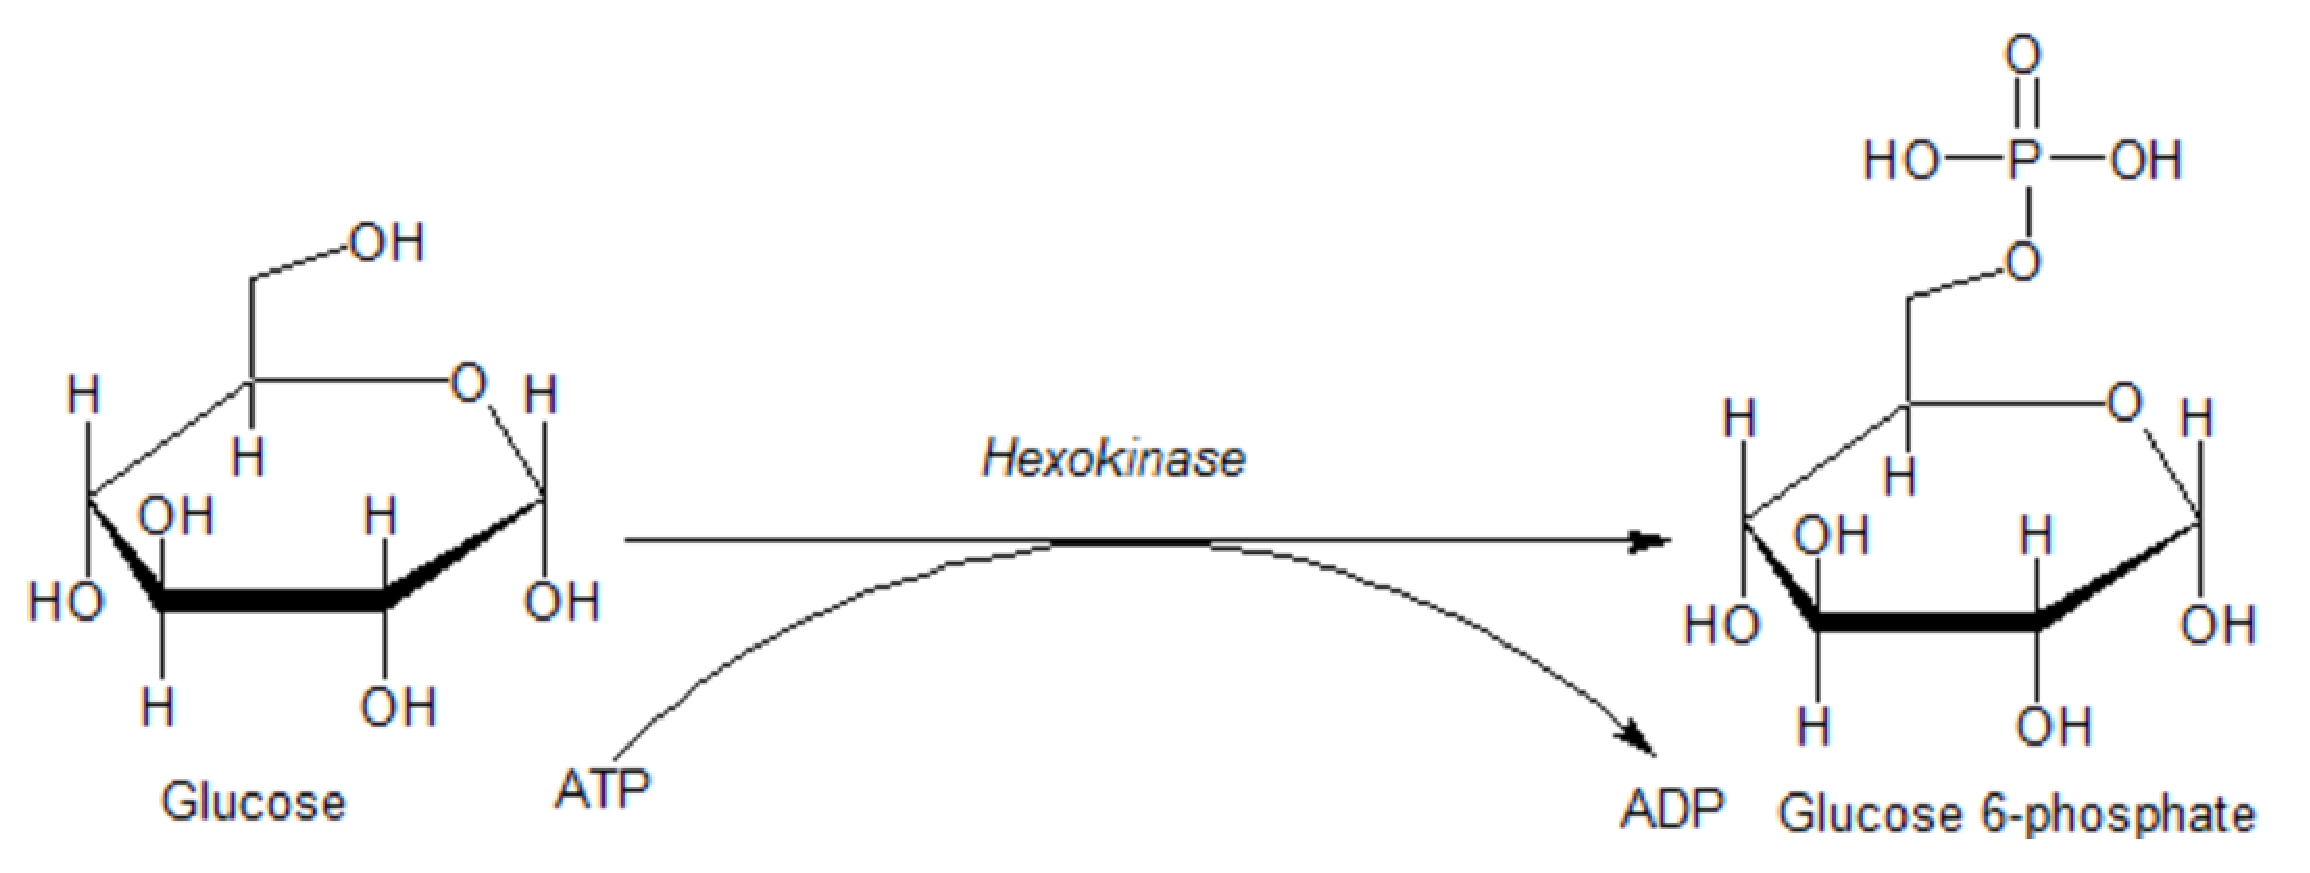
\includegraphics[height=3cm]{./images/Glucose-6P-production.eps}}
  \caption{Glucose-6P production}
  \label{fig:Glucose-6P-production}
\end{figure}

Elevated blood glucose concentrations result in increased intracellular levels
of glucose 6-phosphate in liver, skeletal muscle, and adipose tissue.

Once created, Glucose-6P can involve in the glycolysis -
Sect.\ref{sec:glycolysis}, or can be converted into glucose storage molecules,
such as glycogen or starch.

\begin{enumerate}
  \item to {\bf pyruvate} via glycolysis -  (Sect.\ref{sec:glycolysis}).
  
  \item to {\bf glycogen} for later use - Sect.\ref{sec:glycogen}: 
  
  
  \item to {\bf ribose 5-phosphatase} by pentose phosphate pathway (PPP): 
  leading to the production of reducing equivalent in the form of NADPH.

NOTE: PPP and glycolysis are linked at the level of glyceraldehyde-3-phosphate
(GA3P) and fructose-6-phosphate (fructose-6P)

\end{enumerate}

\subsection{-- G6Pase}
\label{sec:Glucose-6-phosphatase}

Glucose-6-phosphatase (G6Pase), an enzyme found mainly in the liver and the
kidneys, plays the important role of providing glucose during starvation.
Its free-energy change upon dephosphorylation is $\Delta G^\circ = -13.8 $
(kJ/mol). See comparison: Sect.\ref{sec:ATP-overview}.

Unlike most phosphatases acting on water-soluble compounds, G6Pase is a
membrane-bound enzyme, being associated with the endoplasmic reticulum (review:
Schaftingen, Gerin, 2002).

\subsection{-- Glucose-6-phosphate dehydrogenase}
\label{sec:Glucose-6-phosphate-dehydrogenase}

{\bf Glucose-6-phosphate dehydrogenase (G6PD)} deficiency is a condition in
which red blood cells break down (i.e. hemolysis) when the body is exposed to
certain drugs or the stress of infection. It is hereditary which means it is passed down in
families. G6PD deficiency occurs when a person is missing or does not have
enough of an enzyme called glucose-6-phosphate dehydrogenase. This enzyme helps
red blood cells work properly.

\subsection{Fructose-6P}
\label{sec:Fructose-6P}
\label{sec:Fructose-6-phosphate}

Fructose 6-phosphate (or Neuberg ester as it was found by Carl Neuberg in 1918)
is a 6-carbon molecule that is an intermediate during glycoslysis -
Sect.\ref{sec:glycolysis}. It is converted from 

\begin{enumerate}
  \item  Glucose-6P using Glucose-6-phosphate isomerase enzyme

{\tiny
\begin{verbatim}
Glucose-6P --[Glucose-6-phosphate isomerase]--> Fructose-6P
\end{verbatim}
}
  \item Fructose (Sect.\ref{sec:Fructose})
\end{enumerate}

It is further phosphorylated into fructose-1,6-bisphosphate
(Sect.\ref{sec:fructose-1,6-bisphosphate}) using enzyme Phosphofructokinase.

\subsection{-- fructose-1,6-bisphosphate}
\label{sec:fructose-1,6-bisphosphate}

Fructose 1,6-bisphosphate (or Harden-Young ester) , is a 6-carbon molecule that is an intermediate during glycoslysis -
Sect.\ref{sec:glycolysis}

{\tiny
\begin{verbatim}
Fructose-6P  + ATP + H2O  <--[Phosphofructokinase]--->    Fructose-1,6-biphosphate + ADP + Pi
\end{verbatim}
}



\subsection{Ketone bodies}
\label{sec:ketone-bodies}

Ketone bodies are three water-soluble molecules produced by the liver from fatty
acids during periods of low food intake (fasting), starvation, prolonged intense
exercise, etc., after the liver glycogen stores have been depleted (these
glycogen stores are depleted after only 24 hours of fasting).
Ketone bodies are then released into the blood by the liver, together with newly
produced glucose.


The level of ketone body concentrations are on the order of 0.5-5 mM whereas the
pathological ketoacidosis is 15-25 mM.

It is produced in the liver, but is not used by the liver as the liver lacks the
enzyme $\beta$-ketoacyl-CoA transferase, also called thiophorase. Instead,
ketone bodies are used in the heart, brain and muscle.

\begin{enumerate}
  \item  The heart preferentially utilizes fatty acids as fuel under
normal physiologic conditions. However, under ketotic conditions, the heart can effectively utilize
ketone bodies for this purpose

  \item the brain has an obligatory requirement for some glucose (during the
  initial stages the brain does not burn ketones, since they are an important
  substrate for lipid synthesis in the brain)
  
After the diet has been changed to lower blood glucose utilization for 3 days,
the brain gets 25\% of its energy from ketone bodies.

After about 4 days, this goes up to 70\%.

\end{enumerate}

Ketone bodies can be used as fuels, yielding 2 GTP and 22 ATP molecules per
acetoacetate molecule when oxidized in the mitochondria.

Example of ketone bodies:
\begin{enumerate}
  \item acetone

Acetone in low concentrations is taken up by the liver and undergoes
detoxification through the methylglyoxal pathway which ends with lactate

 Acetone in high concentrations due to prolonged fasting or a ketogenic diet is
absorbed by cells other than those in the liver and enters a different pathway via 1,2-propanediol

  \item Ketones produced from omega-3 fatty acids may reduce cognitive
  deterioration in old age.

\end{enumerate}


NOTE: Sect.\ref{sec:Acetyl-CoA}
\begin{verbatim}
ketone bodies  ---[recoverted]---> acetyl-CoA
\end{verbatim}


\begin{itemize}
  \item check adipose tissue - Sect.\ref{sec:adipose-tissue}
\end{itemize}



\subsection{Lactate (lactic acid)}
\label{sec:lactate}
\label{sec:lactate-acidosis}

Lactic acid has the formula ($\ce{C3H6O3}$ or $\ce{CH3-CH(OH)-CO2H}$).
However, with the neutral pH maintained by the body, most lactic acid will be
present in the blood as lactate ($\ce{CH3-CH(OH)-CO2^-}$) with the involvement
of oxygen. NOTE: Lactic acid needs to be converted into lactate using oxygens.

\begin{mdframed}
{\bf lactic acidosis} refers to the build up of lactate (especially L-lactate)
to a level of lactate that is high enough to disrupt a person's acid-base (pH)
balance, i.e. low pH. Lactate acidosis is a subtype of metabolic acidosis -
Sect.\ref{sec:metabolic-acidosis}.

In 1925, Clausen identified the accumulation of lactic acid in blood as a cause
of acid-base disorder. Later, Huckabee's seminal work firmly established that
{\bf lactic acidosis} frequently accompanies severe illnesses and that tissue
hypoperfusion underlies the pathogenesis.
In 1976, Cohen and Woods classified the causes of lactic acidosis according to
the presence or absence of adequate tissue oxygenation.

\end{mdframed}

\begin{enumerate}
  \item In early 19th century, Berzelius found acid lactic - an acid found in
milk, in the muscle of a hunted stag.

  \item In 1907, Fletcher and Hopkins discovered that lactate only found in
fatigued muscle (but not in the recovered one) in the presence of oxygen

This suggests lactate is produced when extreme energy is needed.

  \item \ldots Sect.\ref{sec:history-energy-metabolism-mechanism}
\end{enumerate}

\subsection{-- production of L-lactate (Cori cycle, lactic acid cycle)}
\label{sec:Lactate-production}
\label{sec:lactic-acid-cycle}
\label{sec:Warburg-effect}

Remember that inside a cell, lactate is a product from pyruvate
(Sect.\ref{sec:pyruvate}).
At normal condition, the conversion is a small fraction of pyruvate created.

\begin{itemize}
  \item  During ischaemia, oxygen supply is insufficient to support
  mitochondrial ATP synthesis, and thus flux through the electron transport chain is reduced. In
this scenario, pyruvate oxidation is decreased and thus pyruvate stay longer
in the cytosol, where it gets conversion to L-lactate more, i.e. increase
lactate production.

Because of that, when tissue oxygenation is insufficient, or when the
mitochondrial function is impaired the lactate/pyruvate (La/Py) ratio will
increase (Sect.\ref{sec:lactate-pyruvate-ratio}).

  \item Certain cell types also engage in a form of glucose metabolism known as
  aerobic glycolysis in which glycolysis-derived pyruvate is converted to
  lactate even when oxygen is adequate for pyruvate oxidation.
  
This seemingly wasteful decision is a common component of the metabolic
alterations in a variety of cancers. 
No discussion of cancer metabolism, especially one focusing on pyruvate, would
be complete without a reference to Otto Warburg and his observation (in
1927) that tumor cells utilize aerobic glycolysis, subsequently named the
'Warburg effect'.

Currently there is intense interest in understanding what role the Warburg
effect plays in cancer initiation and growth, with therapeutics being developed
in the hope of reversing metabolic changes required by the cancer cells.
\end{itemize}

L-lactate then can be converted to glucose via the so-called {\bf Cori cycle}
(Sect.\ref{sec:cori-cycle}).

\begin{enumerate}
  \item muscle: produce L-lactate (which can change the pH and making muscle
  fatigue (known as lactic acidosis) - Sect.\ref{sec:lactate})
  
L-lactate is moved to the liver to first prevent lactic acidosis.

  \item at liver: a process called {\bf gluconeogenesis} in that L-lactate is
  converted back to glucose, by using 6 ATP molecules for every L-lactate
  conversion.

The glucose molecules generated are transfered back to muscle for generating
ATP molecules.
\end{enumerate}

NOTE: in cell culture with fermentation, about 50-100\% of glucose is converted
to L-lactate.

% Lactic acid (essentially L-lactate)
% is produced as the by-product of glycolysis - Sect.\ref{sec:glycolysis}.



\subsection{--- isoforms: L-lactate and D-lactate}

Lactate has 2 forms: L-lactate and D-lactate. Both forms (stereoisomers) of
lactate are produced from and metabolized to pyruvate by the action of the
enzyme lactate dehydrogenase (LDH) - Sect.\ref{sec:lactate-dehydrogenase}.
However, the enzyme is isomer-specific so that production and metabolism of
D-lactate requires D-LDH and L-lactate requires L-LDH.

\begin{itemize}

  \item {\bf Mammalian cells only contain L-LDH}.

However, it is now clear that despite the absence of D-LDH, D-lactate is both
produced and metabolized within human cells, albeit in tiny amounts compared to
that of L-lactate.

  
  \item  Carbohydrate-fermenting bacterial species (e.g. lactobacillus spp) can
  produce both D-lactate and L-lactate.
\end{itemize}

\subsection{-- L-lactate}
\label{sec:L-lactate}

In all vertebrates, including humans, the L-lactate form is by far the most
abundant and pathophysiologically significant, and it is this form that is
specifically measured by the lactate sensors.

\textcolor{red}{In health around 1500 mmol of lactate is produced daily and so
long as normal rate of metabolic disposal - principally by the liver and kidneys - is
maintained, blood plasma concentration for L-lactate remains within the
approximate reference range of 0.5-1.5 mmol/L}.

Abnormal increase in plasma lactate (the symptom called {\bf hyperlactatemia})
occurs if the rate of production exceeds the rate of disposal of L-lactate. 
\begin{enumerate}
  \item  (most common) due to reduced oxygen delivery to tissue cells
  ({\bf tissue hypoxia}).

 Tissue hypoxia, which is the result of inadequate perfusion of tissues and/or
reduced blood oxygen (hypoxemia), is a common feature of many kinds of
critical illness so that lactate measurement is most frequently used to
monitor tissue oxygenation in the critically ill.
  
  \item 
\end{enumerate}


If hyperlactatemia is sufficiently severe (plasma lactate >5.0 mmol/L), it is
associated with acidosis (blood pH <7.35). The condition is then called lactic
acidosis.


\subsection{-- D-lactate}
\label{sec:D-lactate}

D-lactate is 100x smaller in amount that L-lactate in human's blood, due to the
lacking of D-LDH enzyme. However, in other species, it can be different
(Sect.\ref{sec:lactate}). 

NOTE: D-lactate normally present in the blood of humans (concentration 5-20
$\mu$mol/L in healthy adults compared to 1000 $\mu$mol/L, i.e. 1.0 mmol/L for
L-lactate).
\url{http://acutecaretesting.org/en/articles/l-lactate-and-d-lactate-clinical-significance-of-the-difference}

\subsection{-- Cori cycle}
\label{sec:cori-cycle}

L-lactate can be a source of energy. 
In muscle, having high level of L-lactate can fatigue the muscle. 
Carl Ferdinand Cori and Gerty Cori discovered the metabolic pathway that help
converting {\bf lactate} back to glucose for replenishing the glucose needed by
muscle.

In particular, L-lactate produced is moved to liver and is converted back to
glucose before transmitting to the muscle that the muscle
can use for energy production.
\url{https://en.wikipedia.org/wiki/Cori_cycle}

In the brain, astrocyte for neurons plays the role of liver for muscle.
This is the lactate-shuttle hypothesis. 
(Sect.\ref{sec:lactate-shuttle-hypothesis}).


\subsection{-- lactate shuttle hypothesis}
\label{sec:lactate-shuttle-hypothesis}

REVIEW: There are two major working models
\begin{enumerate}
  \item {\bf classical view}: both neurons and astrocytes can utilize glucose as
  the energy source through oxidative metabolism
  
  \item {\bf astrocyte-neuron lactate shuttle hypothesis} (ANLSH): astrocyte
  which can consume glucose through anaerobic glycolysis to pyruvate and then to lactate
  
The lactate is secreted to the extracellular space to be taken up by the neuron
for further oxidative degradation. Sect.\ref{sec:lactate-oxidation} describes
the conversion from lactate to pyruvate.

As the foot of astrocytes closed to the capillaries, it is probably truth
that astrocyte is the first to get glucose.

\end{enumerate}

Genc, Ozilgen (2011) showed that in both normal, and hypoxia-conditions, ANLSH
model does indeed provide the neuron with more ATP than in the classical view.
%https://bmcsystbiol.biomedcentral.com/articles/10.1186/1752-0509-5-162


\textcolor{red}{Recently, lactate has been found to function not only as a
energy source, but also a signaling molecule}, i.e.
causes cells in the brain to release more noradrenaline (norepinephrine in US
English - Sect.\ref{sec:noradrenalin}), a hormone and neurotransmitter
which is fundamental for brain function.

\subsection{-- lactate oxidation: from lactate to pyruvate}
\label{sec:lactate-oxidation}

{\bf Lactate oxidation} is the process converting lactate back to pyruvate
(Sect.\ref{sec:pyruvate}). This process is important for astrocyte-neuron
lactate shuttle hypothesis (Sect.\ref{sec:lactate-shuttle-hypothesis}).

\subsection{-- lactate/pyruvate ratio (La/Py ratio)}
\label{sec:lactate-pyruvate-ratio}


As lactate and pyruvate are equally permeable across the cell membranes the
La/Py ratio measured in the intercellular space will give true information
regarding the cytoplasmatic redox state.

La/Py ratio is an important biomarker in Lund concept for neurocritical care
(Sect.\ref{sec:Lund-concept}).


\subsection{Glycogen}
\label{sec:glycogen}

The liver (Sect.\ref{sec:liver}) helps to maintain a constant level of blood
sugar. If the blood sugar increases, e.g. after having meal, the liver removes
excess sugar by converting to glycogen. 

Glycogen is formed from Glucose-6P inside the cells, serving as long-term energy
storage. So that when the cell needs to generate ATP, but glucose source from
outside is not readily available, it can quickly convert glycogen back into
glucose (Sect.\ref{sec:gluconeogenesis}).

The formation and breakdown of glycogen do not occur in a single
reversible reaction, but in 2 different pathways.

{\bf Metabolism}: FORMATION of GLYCOGEN, i.e. glycogenesis: from Glucose-6P
\label{sec:glycogenesis}  
\begin{itemize}
  
\item glucose-6-phosphate is isomerized to glucose-1-phosphate by {\it
    phosphoglucomutase}. 

\item glucose-1-phosphate react with
  UTP\footnote{uridine triphosphate} to form
  UDPG\footnote{uridine diphosphate glucose}, and release $PP_i$
  ({\it pyrophosphate} - Sect.\ref{sec:pyrophosphate}.

\item UDPG is transformed into glycogen, and release UDP. 
\end{itemize}

{\bf Breakdown}: gluconeogenesis - Sect.\ref{sec:gluconeogenesis}
\begin{itemize}
\item glycogen is broken down into glucose-1-phosphate by {\it
    phosphorylase} 
\end{itemize}


% Carbohydrate is stored in the heart as {\bf glycogen} - the secondary
% long-term energy storage. 
\begin{enumerate}
  \item In liver: glycogen makes up  5-6\% of the organ's fresh weight (100-120
  g in an adult).

NOTE: Only glycogen stored in the liver can be made accessible to other organs.
  
  \item  In muscle, glycogen is found in low concentration (1-2\% of the muscle
  mass)

  \item In skeletal muscle

  \item in kidneys: a small amount of glycogen is found
    
  \item in white blood cells: a small amount
  
  \item in astrocytes: a small amount 
  
  NOTE: in astrocytes, glucose-6P can also be used to store
glucosyl units as glycogen.
  
  \item the uterus also stores glycogen during pregnancy to nourish the embryo
\end{enumerate}
The amount of glycogen stored in the body-especially within the muscles, liver,
and red blood cells - mostly depends on physical training, basal
metabolic rate, and eating habits 


\section{GI (glycemic index): blood glucose level}
\label{sec:glycemic-index}

Some foods break down more quickly than others, causing a rapid -- and
undesirable -- spike in blood glucose, an effect that's expressed as each food's
"glycemic index" or GI.

The smaller GI the less impact of the food on the undesired spike in
blood glucose. NOTE: GI <= 55 (good); 56-69 (medium), 70-higher (bad).

\begin{itemize}
  \item  a boiled potato has a considerably higher GI than an apple. 
  
  \item food with high GI: potatoes, white rice, and white bread
  
\end{itemize}

The fact a food has a low glycemic index doesn't mean it's super-healthy, or
that you should eat a lot of it. Calories, vitamins, and minerals are still
important. For example, potato chips have a lower glycemic index than oatmeal
and about the same as green peas. But oatmeal and green peas have more
nutrients.

\chapter{Cell-specific energy production}


\section{How energy is stored in cells }
\label{sec:high-energy-compound}

Energy is handled within cells in the form of high energy phosphate bonds.
The principle behind this is that some chemical bonds need a lot of energy to be
welded. Adding one phosphate group (P) to adenosine-mono-phosphate creates such
a high energy bond. The resulting compound is adenosine-di-phosphate, or ADP.
Repeat this, and you get another high energy bond, the compound being called by
analogy adenosine-tri-phosphate or ATP. Conversely, if you have an ATP and
remove one P, you get ADP, P, and some energy, which in turn may be used for all
sorts of energy requiring tasks, like ion pumping or contracting special
proteins. 

Example of high-energy compounds (i.e. containing phosphate bond)
\begin{itemize}
  \item ATP - Sect.\ref{sec:ATP-overview}, i.e. ATP-ADP system 
  
  \item phosphocreatine - Sect.\ref{sec:phosphocreatine}, i.e. PCr-Cr system

  \item GTP - Sect.\ref{sec:GTP}
   
   \label{sec:PEP}
   \label{sec:1,3-BGP}
  \item In cells, there are some compounds with higher phosphoryl transfer
potential than ATP, e.g. : PEP, 1,3-BGP. It means that they can easily transfer
the phosphoryl group to ADP to form ATP.

\begin{equation}
  \label{eq:4}
  1,3-PGB + ADP \ce{->} 3-\text{phosphoglyceric acid} + ATP
\end{equation}

\begin{framed}
  Some biosynthesis reactions are driven by molecules other than ATP,
  e.g. GTP (guanosine triphosphate), UTP (uridine triphosphate), CTP
  (cytidine triphosphate).  The diphosphate forms of these molecules
  are GDP, UDP, and CDP. The monophosphate forms of these molecules
  are GMP, UMP, and CMP. 

  There are derivatives of ATP, that serves as important electron
  carriers: \ce{NAD+}, and \ce{FAD}.  Another energized biomolecule is
  {\it nicotinamide adenine dinucleotide phosphate} (NAD+PH) used in
  anabolic reactions (e.g. in lipids or nucleic acids synthesis).
  NAD+PH is the reduced form of NAD+P+, or NAD+P+ is the oxidized form
  of NAD+PH.

\end{framed}



\end{itemize}

As ATP is the high-energy storage molecule, it needs to be created, and then
release to the cytosol to provide energy for other cellular processes.
\begin{itemize}
  \item ATP can be created inside cytosol, either via phosphagen system -
  Sect.\ref{sec:phosphagen-system} or glycolytic system -
  Sect.\ref{sec:ATP-production-in-cytosol-via-glycolytic-system}
  
  \item ATP is mainly created inside mitochondria -
  Sect.\ref{sec:ATP-production-inside-mitochondria}
\end{itemize}

To create ATP (Sect.\ref{sec:ATP-overview}), cells need to have some energy
substrates (Sect.\ref{sec:energy-substrates}). First, glucose or glutamate needs
to be transported from blood vessels into extracellular space, and then from
there into the cells via either SGLT (Sect.\ref{sec:SGLT}) and GLUT
(Sect.\ref{sec:GLUT}).

When a cell needs to generate ATP, depending on the cell types, the cell can
utilize (1) glucose that circulates in the blood, or (2) glycogen -
Sect.\ref{sec:glycogen} stored if the cells is myocyte (i.e.
in the muscles) and or hepatocyte (i.e. the liver). It is recommended to know
Sect.\ref{sec:enery-production-pathways}.

In the fasted state or during exercise, fuel substrates (e.g. glucose and TAG)
are released from the liver into the circulation and metabolized by muscle,
adipose tissue, and other extrahepatic tissues.

Every day your body carries out many nonspontaneous reactions. As discussed
earlier, if a nonspontaneous reaction is coupled to a spontaneous reaction, as
long as the sum of the free energies for the two reactions is negative, the
coupled reactions will occur spontaneously

\section{Glucose transporters}
\label{sec:glucose-transporters}


\subsection{SGLT}
\label{sec:SGLT}

Sodium dependent glucose transporters (SGLTs) which transport glucose against
its concentration gradient



\subsection{GLUT}
\label{sec:GLUT}

The GLUT proteins are the facilitative glucose transporter family, i.e. uptake
glucose from blood into the cell and release glucose from cell back into the
blood. Depending on the cell types, different isoforms may be involve in such
functionality.

Unlike SGLT (Sect.\ref{sec:SGLT}), GLUT's activity is sodium-independent and
only enable glucose diffusion along its concentration gradient.

There are total 14 genes encoding GLUT proteins.
\begin{enumerate}
  \item GLUT1 - Sect.\ref{sec:GLUT1}
  \item GLUT2 - Sect.\ref{sec:GLUT2}
  \item GLUT3 - Sect.\ref{sec:GLUT3}
\end{enumerate}

\subsection{GLUT1}
\label{sec:GLUT1}

The GLUT 1 isoform of the facilitative glucose transporter family is expressed
in the blood-brain barrier; however, the major glucose transporter isoform(s) in
neurons and glia are mainly GLUT3. 

GLUT1 (Glucose transporter 1) facilitates the transport of glucose across the
capillaries and plasma membranes of astrocytes.

{\tiny
\begin{verbatim}
glucose (capillary) --[GLUT1]---> glucose (endothelial cell) --[GLUT1]--> 
     interstitial fluid (ISF)
\end{verbatim}
}

GLUT1 occurs in brain in two isoforms
\begin{enumerate}
  \item  more glycosylated GLUT1 is produced in brain microvasculature and
  ensures glucose transport across the blood brain barrier (BBB)
  
  \item less glycosylated form is localized in astrocytic end-feet and cell
  bodies and is not present in axons, neuronal synapses or microglia
\end{enumerate}
Glucose transported to astrocytes by GLUT1 is metabolized to lactate serving to
neurons as energy source. 

GLUT1 is highly conserved, e.g. GLUT 1 of humans and mice have 98\% identity at
the amino acid level. 

Proinflammatory cytokine interleukin (IL)-1$\beta$ upregulates GLUT1 in
endothelial cells and astrocytes,  whereas it induces neuronal death in neuronal
cell culture.

\subsection{GLUT2}
\label{sec:GLUT2}

GLUT2 is found in hepatocyte (Sect.\ref{sec:hepatocyte}).

GLUT2 is present in hypothalamic neurons and serves as a glucose sensor in
regulation of food intake.

In neurons of the hippocampus, GLUT2 is supposed to regulate synaptic activity
and neurotransmitter release.

\subsection{GLUT3}
\label{sec:GLUT3}

GLUT3 has shown to share 64.4\% identity with GLUT1.
GLUT3 is the most abundant glucose transporter in the brain having five times
higher transport capacity than GLUT1.

GLUT3 is most known for its specific expression in neurons and has originally
been designated as the neuronal GLUT.  It is present in neuropil, mostly in
axons and dendrites. Its density and distribution correlate well with the local
cerebral glucose demands. 

\subsection{GLUT4 and GLUT8}
\label{sec:GLUT4}
\label{sec:GLUT8}

GLUT4 and GLUT8 are insulin-regulated glucose transporters in neuronal cell
bodies in the cortex and cerebellum, but mainly in the hippocampus and amygdala,
where they maintain hippocampus-dependent cognitive functions (Jurcovicova,
2014). GLUT4 is also the main glucose transporters in the heart. 

Insulin translocates GLUT4 from cytosol to plasma membrane to transport glucose
into cells, and GLUT8 from cytosol to rough endoplasmic reticulum to recover
redundant glucose to cytosol after protein glycosylation.

The activity of GLUT4 is mediated by myocardial contraction, as cardiomyocytes
are constantly contracting it is likely that contraction mediated GLUT4
translocation represents an important mechanism that governs the entry of
glucose into the heart. While this is also true in skeletal muscle, because many
muscles are often at rest, insulin mediated GLUT4 translocation represents a
quantitatively more important mechanism regulating skeletal muscle glucose
uptake than is the case in the heart (Abel, 2004). 
%https://www.ncbi.nlm.nih.gov/pubmed/14766360


\subsection{GLUT5 (fructose transporter)}
\label{sec:GLUT5}

GLUT5 is predominantly fructose transporter. 

 In brain, GLUT5 is the only hexose transporter in microglia, whose regulation
is not yet clear. It is not present in neurons.

\section{Muscle}
\label{sec:heart-energy-substrate}

Muscle breaks down glycogen and proteins and releases lactate and alanine.
Alanine, lactate, and glycerol are delivered to the liver and used as precursors
to synthesize glucose (gluconeogenesis)

NOTE: In heart, 10-30\% of ATP is generated by glucose and lactate (i.e.
carbohydrate); and 60-70\% from fatty acids (Sect.\ref{sec:fats}). The heart can
also utilize amino acids and ketones instead of fatty acids.

Although glucose is not the major metabolic substrate in the heart at rest,
there are many circumstances in which it assumes greater importance such as
during ischemia, increased workload and pressure overload hypertrophy.

Like all other cells, glucose is transported into cardiac myocytes by members
of the family of facilitative glucose transporters (GLUTs), in that
the most abundant glucose transporter in the heart is the GLUT4 transporter
(Sect.\ref{sec:GLUT4}).

In contrast to skeletal muscle, where most GLUT1 is in perineural sheaths (1),
in the heart there is significant expression of GLUT1 (2), which under certain
circumstances is responsible for a significant component of basal cardiac
glucose uptake (Abel, 2004).   

\subsection{How the heart generate ATP}

There are different ways of generating ATP energy utilized by the hearts
\begin{enumerate}

\item oxidation of fats (only under well-oxygenated heart)

\item carbohydrate metabolism (from glucose, under both anaerobic and
  aerobic conditions)

  \begin{itemize}
  \item {\it glycolysis} (not requiring oxygen) has limited capacity to
  regenerate ATP and cannot meet the energy demand of beating
    heart\footnote{which explain an interruption in oxygen supply in
      only a minute can halt the contraction}
      
As this process also needs ATP, ATP regenerated by glycolysis ({\it glycolytic
ATP}) play a special role in supplying needs of key energy-consuming reactions.

  \item {\it oxidative metabolism} (require oxygen) play a key role in producing
  large number of ATP. 
  \end{itemize}

\item amino acid metabolism (contribute little)

\end{enumerate}


\begin{framed}
\begin{verbatim}
  glucose -->(10 linked reactions)--> pyruvate 
 
  pyruvate --[anaerobic]--> lactate
  pyruvate --[aerobic]--> Acetyl CoA
\end{verbatim}
During the 10 linked reactions, the released carbons are subsequently
oxidized to \ce{CO2}. 

\end{framed}

\subsection{Heat production in muscle}
\label{sec:heat-production-in-muscle}

Hill (who was awarded Nobel prize in 1922 for his work in heat production in
muscle. He proposed the four phases of heat-production of muscle.




\section{Liver cell (hepatocyte)}
\label{sec:hepatocyte}

Liver energy metabolism is tightly controlled. Multiple nutrient, hormonal, and
neuronal signals have been identified to regulate glucose, lipid, and amino acid
metabolism in the liver. Dysfunction of liver signaling and metabolism causes or
predisposes to nonalcoholic fatty liver disease (NAFLD) and/or type 2 diabetes.

Hepatocytes are the main cell type in the liver (~80\%). Blood glucose enters
hepatocytes via GLUT2 - Sect.\ref{sec:GLUT2}. Hepatocyte-specific deletion of
GLUT2 blocks hepatocyte glucose uptake.

GLUT2 also mediates glucose release from the liver; however, deletion of GLUT2
does not affect hepatic glucose production in the fasted state,  suggesting that
glucose is able be released from hepatocytes through additional transporters
(e.g. GLUT1) or by other mechanisms.


\section{Brains: Neurons and Astrocyte}
\label{sec:brain-energy-substrate}

What is the preferred energy source for brain and erythrocytes? - {\bf Glucose}
- Sect.\ref{sec:glucose}.  Glucose is transported from blood vessels/capillaries
through the blood-brain barrier (BBB) via transporters. In the brain, both types
of transporters (GLUT and SGLT) are present with different function, affinity,
capacity, and tissue distribution.

Nevertheless, under particular circumstances the brain has the capacity to use
other blood-derived energy substrates, such as ketone bodies during development
and starvation (Nehlig, 2004 and Magistretti, 2008) -
Sect.\ref{sec:ketone-bodies}) or lactate during periods of intense physical
activity (van Hall et al., 2009) - Sect.\ref{sec:lactate}.


\begin{itemize}
  \item More glycosylated form GLUT1: found on brain microvasculature
  
  \item The less glycosylated form GLUT1 is localized in astrocytic end-feet and
  cell bodies and is not present in axons, neuronal synapses or microglia. Glucose
  transported to astrocytes by GLUT1 is metabolized to lactate serving to
  neurons as energy source.   
  
  \item GLUT5 is predominantly fructose transporter. In brain, GLUT5 is the only
  hexose transporter in microglia, whose regulation is not yet clear. It is not
  present in neurons 
\end{itemize}
 
The GLUT 1 isoform is expressed on the membrane of brain microvasculature and to
ensure glucose can pass the blood-brain barrier
(Sect.\ref{sec:blood-brain-barrier}); however, the major glucose transporter
isoform(s) in neurons and glia are mainly GLUT3 (Sect.\ref{sec:GLUT3}).
Glucose passes to the astrocytes via GLUT1 (Sect.\ref{sec:GLUT1}).


\begin{verbatim}
Glucose -[blood-brain-barrier, BBB via 
           glycosylated GLUT1]--> extracellular space

Glucose in extracellular space then
1.	---[less glycosylated GLUT1]---> into astrocyte 
2.	---[GLUT3]--> into neuron

Astrocyte: produce lactate --> released into extracellularspace

a.	Lactate -[...]--> into neuron


3.	---[SGLT (sodium-dependent glucose transporter)]--> into neuron
       (transport glucose against its 
       concentration gradient)

// fasting condition (i.e. no food)
Ketone bodies ---> neurons/astrocytes
\end{verbatim} 

Some cells, e.g. nerve cells, have limited storage capacities for either glucose
or ATP. Thus, a constant supply of glucose is fairly important to the normal
function of the neurons.  

Recent evidences have confirmed the 20-year old hypothesis from the
1990's postulates, that a well-orchestrated collaboration between two cell
types, astrocytes and neurons, is the basis of brain energy metabolism.
In particular, nerve cells cover their high energy demand with glucose and
lactate (Sect.\ref{sec:lactate}).
Glucose transported to astrocytes by GLUT1 is metabolized to lactate serving to
neurons as energy source.


% \begin{mdframed}
% Glucose is transported across the membrane via 2 types of transporters: sodium
% dependent glucose transporters (SGLTs) which transport glucose against its
% concentration gradient and 2) sodium independent glucose transporters (GLUTs),
% which transport glucose by facilitative diffusion in its concentration gradient.
% 
% In the brain, both types of transporters are present with different function,
% affinity, capacity, and tissue distribution.
% 
% Glucose transported to astrocytes by GLUT1 is metabolized to lactate serving to
% neurons as energy source. 
% \end{mdframed}


 
\subsection{How the brain generate ATP}

Together with the heart, liver, and kidneys, the brain consumes about 60\% of
the body's energy requirements.
\begin{itemize}
  \item  At rest, it uses approximately 20\% to 23\% of the body's total energy
  requirements, despite accounting for only 2\% of the body's mass.
  
  \item Almost all of that oxygen is used to oxidize glucose to carbon dioxide
  and water.
\end{itemize}

There is no storage of energy in the brain, except the very little energy stored
as glycogen (Sect.\ref{sec:glycogen}). As a result, the brain relies almost
entirely on circulating glucose for fuel via the blood vessels. Once inside the
neurons, glucose is metabolized inside the cytosol; then one of the product, the
pyruvate migrate into the mitochondria for further energy production in a number
of steps to produce cellular energy, or ATP.

Most of the glucose consumed by the brain is used to maintain synaptic function
and resting potential of neurons. The energy requirements of different types of
neurons varies.
\begin{itemize}
  \item  Large-projection neurons with relatively long axons are most affected
  by Alzheimer's disease and these neurons generally have high energy requirements.
  
  \item 
\end{itemize}



\section{Cultured cells}
\label{sec:tissue-culture-energetic-demand}

Tissue cultures is dissed in Sect.\ref{sec:tissue-culture}.
In this section, we discuss what factors affect cell's energetic demands in
tissue culture.

\subsection{cultured myotubes}

Human primary muscle cells are a widely used model system to study muscle
metabolism and its related disorders.
The oxidative capacity of skeletal muscle is highly influenced by various
genetic and environmental factors; {\bf cultured myotubes} offer a unique model
that separates these two influences on metabolic phenotype

\begin{itemize}
  \item  Cell culture of human primary myotubes offers not only an excellent and
  dynamic model for studying metabolism under standardized conditions, but
  provides an excellent system for studying metabolic disorders. I 

Many studies shown that human primary muscle cells retain the same metabolic
phenotype as those previously evidenced in vivo in muscle

However, cultured muscle cells are highly glycolytic when grown and
differentiated under high glucose conditions relative to muscle tissue in vivo,
complicating the study of mitochondrial dysfunction. Typical cell cultures are
grown with glucose 25mM which is quite high (Sect.\ref{sec:glucose-concentration})

NOTE: different types of cells (e.g., cancer cells, primary fibroblasts) grown
in a medium in which glucose is replaced with galactose show a significantly
increased oxygen consumption rate compared to cells grown in medium containing a
high concentration of glucose (25 mM).  

\end{itemize}
\url{https://www.ncbi.nlm.nih.gov/pmc/articles/PMC3240634/}




%\chapter{Energetics and Energy Production}
\chapter{Important concepts in understanding energy production in cells}
\label{chap:energ-energy-prod}

It is recommended to read Chap. \ref{chap:biochem-intro}, and
Chap.\ref{chap:enzymes}.


\section{Terminology}
\label{sec:terminology}

\begin{itemize}

\item {\it metabolism} = synthesis
  ({\it a linked series of chemical reactions that begins with a
    particular molecule and convert it into some other molecule or
    molecules in a carefully designed fashion}
  - which is also called {\bf metabolic pathway})

\label{sec:catabolism}
\item {\it catabolism} = a reaction in that generate energy
(e.g. the breakdown of glucose by glycolysis (Sect.\ref{sec:glycolysis}) to
create ATP)

\label{sec:anabolism}
\item {\it anabolism} = reactions that require energy

\item {\it amphibolic pathways} = a pathway that can be either
  anabolic or catabolic, depending on the energy condition.
  

\end{itemize}

\begin{framed}

  Metabolic pathways are formed by the coupling enzyme-catalyzed
  reactions such that the overall change free energy of the pathway is
  negative.

  A thermodynamically unfavorable reaction sequence can be converted
  into a favorable one by coupling it to the hydrolysis of a
  sufficient number of ATP molecules in a new reaction.
\end{framed}

\section{Gibbs free energy ($\Delta G_f^\circ$: kJ/mol) and related concepts}

\subsection{Gibbs free energy change ($\Delta
G$: $\Delta G^{\circ}$ and $\Delta G^{\circ'}$)}
\label{sec:Gibbs-free-energy}

We can learn more about {\it Gibbs free energy} in Biophysics-ThermoStat book
(Section on System-State).
Here, we will focus on the change in Gibbs' free energy: $\Delta G$ (kJ/mol.)

NOTE: When talking a value of $\Delta G$, we needs to know the condition it is.
So, typically, standard free energy change ($\Delta G^\circ$) is used in that
$\Delta G$ were calculated for a particular set of conditions known as standard
conditions. For biochemical reactions, standard conditions are generally defined
as 25$^\circ$ C (or 298 Kelvin), 1 M concentrations of all reactants and
products, 1 atm pressure, and pH of 7.0, point.
(NOTE: the prime mark in $\Delta G^{\circ'}$ indicates that pH is included in
the definition).

\textcolor{red}{The conditions inside a cell or organism can be very different
from these standard conditions, so $\Delta G$ values for biological reactions 
{\it in vivo} may vary widely from their standard free energy change}

\begin{itemize}
  \item $\Delta G < 0$:  the reaction in the direction from left to right, is
  spontaneous, i.e. it releases energy and thus no energy needed for the
  reaction to occur.

It is defined as the energy required (kJ) to form one mole of a substance in its
standard state (usually 298.15K or 25$^\circ$C); if the energy required
(kJ/mol) is negative, then the reaction release energy.

Example: plain carbon (C) gives off energy as it combines with oxygen
($\ce{O2}$) - through burning reaction, and concert to carbon dioxides
($\ce{CO2}$).  The CO2 is at a lower energy state than the pure carbon and pure
oxygen were, since the energy was released as heat.
\begin{equation}
\ce{ C + O2 -> CO2 } \qquad; \Delta G = -395 \text{kJ/mol.}
\end{equation}
NOTE: The free energy state of carbon is zero, and free oxygen is also zero; but
the free energy state of $\ce{CO2}$ is -395 kJ/mol.
  
  \item 
\end{itemize}
% = the concept simply says that there is an energy
% level/state associated with the formation of a given compound, and that there is
% a change in energy to go along with the change in chemistry.

\textcolor{red}{Example}: In molecular dynamics study of protein
folding (3D structure), {\bf themodynamic principle} says that 
the amino acid sequence of a protein determines its native structure and the
native structure has the minimum Gibbs free energy (Fang, 2012).
\footnote{\url{https://arxiv.org/abs/1202.1358}}.

\begin{mdframed}
NOTE: There are different calories unit type

\begin{enumerate}
  \item thermochemical/food calorie

1 kJ (kilo Joules) = 0.239006 kcal-th (kilocalories)

1 kcal-th = 4.184 kJ

  
  \item international calorie

1 kcal-IT = 4.1868 kJ
  
  \item 15$^\circ$C calorie

1 kcal$_{15}$ = 4.1855 kJ
  
  \item 20$^\circ$C calorie

1 kcal$_{20}$ = 4.182 kJ

\end{enumerate}
\url{http://www.rapidtables.com/convert/energy/kj-to-kcal.htm}

So the energy: $E_{kcal} = E_{kJ} / 4.184$
\end{mdframed}

References:
\begin{enumerate}
  \item
  \url{https://en.wikipedia.org/wiki/Standard_Gibbs_free_energy_of_formation}
\end{enumerate}

\subsection{Nernst equation to calculate Gibbs free energy}

The energy, electric potential required in a chemical reaction can be calculated
using {\bf Nernst equation}. 
The Nernst equation has broad applications in biology because much of biology
involves electron transfer reactions (Sect.\ref{sec:nernst-equation}).
These reactions are responsible for producing energy and for building and
maintaining structures needed by an organism.

A standard potential E$^\circ$ tables is measured at 1 bar pressure ($\simeq
1$atm), temperature 298$^\circ$K (or 25$^\circ$ or room temperature), and a
concentration of 1.0M for each of the products. In a redox reaction: 
$\ce{aA + bB -> cC + dD}$, then the electric potential in a non-standard condition
\begin{equation}
E = E^\circ - (RT/nF)\ln Q
\end{equation}
with $Q = \frac{C^cD^d}{A^aB^b}$, $n$ = number of electrons transferred. The
free energy is
\begin{equation}
\Delta G = -nFE^\circ
\end{equation}
with $n$ is the number of moles.


\section{redox reaction or coupling reaction}
\label{sec:redox-reaction}
\label{sec:oxidation-reduction-reaction}
\label{sec:coupling-reaction}

The term {\bf Redox} ({\bf RED}uction-{\bf OX}idation) reactions refer to a
family of (dual) reactions that are concerned with the transfer of electrons
(e$^-$) between species. So, a redox reaction involves two parallel processes
\begin{enumerate}
  \item oxidation reaction: removing electron from an electron donor
  (Sect.\ref{sec:reductant})
  \item reduction reaction: transfer the electron to an electron acceptor
(Sect.\ref{sec:oxidant}).
\end{enumerate}

The two reactions must be coupled because you can't have an electron donor
without an electron recipient. Because of this, these two reactions (oxidation
and reduction) are considered to be two halves of a whole. In other words, a
{\bf redox reaction} consists of an oxidation half reaction and a reduction half reaction.

Along with that, the oxidation states (Sect.\ref{sec:oxidation-state}) of
reactants are changed. 

REMEMBER:
\begin{verbatim}
OIL RIG = Oxidation Is Loss; Reduction Is Gained (of electrons)
\end{verbatim}

\begin{mdframed}

Remember that electrons (e$^{-}$) are tiny charged particles that orbit the
nucleus of an atom at dizzying speeds. Depending on how many electrons are
orbiting the nucleus, and in which orbitals (at what distance from the nucleus),
some atoms hold on to some of their electrons very loosely, and have a higher
tendency to give them away.

Some atoms hold onto their electrons very tightly, and are in fact able to
attract nearby electrons into their orbitals.
The potential, or tendency, to gain electrons, is the {\bf reduction potential}.
\end{mdframed}

{\bf Example}: ATP is used as free-energy currency by coupling its (spontaneous)
dephosphorylation with a (nonspontaneous) biochemical reaction to give a net
release of free energy (i.e., a net spontaneous reaction). The underlying force
driving these reactions is the {\bf Gibbs free energy} of the reactants and products
(Sect.\ref{sec:Gibbs-free-energy}, Sect.\ref{sec:gibbs-free-energy-1}).


{\bf Example}: a redox reaction is composed of an oxidation reaction and a
reduction reaction.
\begin{equation*}
\begin{split}
\ce{Cu(s) -> Cu^2+ + 2e-} \\
\ce{2Ag+ (aq) + 2e- -> 2Ag (s)}
\end{split}
\end{equation*}
The symbol e$^-$ represents a free electron. (s) = solid, (aq) = aqueous. 

%{\it Oxidation} refers to the loss of electrons, while {\it reduction} refers
% to the gain of electron.

\subsection{redox pair}
\label{sec:redox-pair}



%%TUANTUANTUAN
\subsection{Oxidation (gaining oxygen, removing hydrogen, increase in oxidation
number or loosing electron) vs.
Reduction (losing oxygen, adding hydrogen, decrease in oxidation number, or
gaining electron)}
\label{sec:oxidation}
\label{sec:reduction}

{\bf NOTE}: Remember OIL RIG term.

\begin{itemize}
  \item  {\bf oxidation} (gaining oxygen) = the process in that a molecule
  looses an electron (i.e. lost energy) = a molecule increases its oxidation state.

  See oxidation state - Sect.\ref{sec:oxidation-state}. \textcolor{blue}{The
  term 'oxidation' originally means a reaction of a substance with oxygen
by Lavoisier; much later, it was realized that the substance, upon being
oxidized (or gaining oxygen), loses electrons, and the use of the term
"oxidation" was extended to include other reactions in which electrons are
lost.}

A molecule that looses electron is called a {\bf reducing agent} (or {\bf
reductant}).

  \item {\bf reduction} (losing oxygen, or adding hydrogen) = the process in
  that a molecule that gains electron (i.e. increase energy); therefore reducing
  oxidation number/state - Sect.\ref{sec:oxidation-state}.

A molecule that gain electrons is called {\bf oxidizing
molecule} (or {\bf oxidant}).
\end{itemize}


\subsection{Reductant (reducing agent, electron donor) vs. Oxidant (oxidizing
agent, electron acceptor)}
\label{sec:reductant}
\label{sec:oxidant}
\label{sec:reducing-agent}

As pointed in Sect.\ref{sec:oxidation}, the {\bf reductant} (or reducing agent,
reducer, or electron donor) is an element or compound that loses (or donate)
electrons to another chemical species in a {\bf redox chemical reaction} -
Sect.\ref{sec:redox-reaction}.

\begin{itemize}

  \item Since the reductant is losing electrons, after the reaction, it is said
  to have been {\bf oxidized} - or the agent goes through the {\it oxidation}
  process (Sect.\ref{sec:oxidation}), and it increases the oxidation number.

  \item A reductant is typically in one of its lower possible oxidation states -
Sect.\ref{sec:oxidation-state} and thus it can donates electrons to another
chemical species of higher oxidation state; so that its oxidation state can
increase.

\end{itemize}

As pointed in Sect.\ref{sec:oxidation}, the {\bf oxidant} (or oxidizing agent,
or electron acceptor) is typically at higher oxidation state than the reductant,
and once they interacts; the oxidant can gains electrons and its oxidation
state is {\bf reduced}.

Example:
\begin{enumerate}
  \item NADH
  \item \ce{FADH_2}
\end{enumerate}

\subsection{Oxidiation state (oxidation number)}
\label{sec:oxidation-state}


The oxidation state, often called the oxidation number, is an indicator of the
degree of oxidation (i.e. loss of electrons - Sect.\ref{sec:oxidation}).
FACTS:
\begin{enumerate}
  \item Oxidation states are typically represented by integers

  \item The molecule with many electrons has low oxidation number; and once it
  donates electrons, the new molecule then has a higher oxidation number.
   
  \item  The highest known oxidation state is reported to be +9 in
  $\ce{IrO_4^+}$ (iridium tetroxide)

  \item The lowest known oxidation state is -5 for boron, gallium, indium, and
  thallium

  \item The increase in oxidation state of an atom, through a chemical reaction
  that the molecule loosing electrons, is known as an oxidation -
  Sect.\ref{sec:oxidation}

  \item The decrease in oxidation state is known as a reduction -
  Sect.\ref{sec:reduction}
\end{enumerate}

RULE:
\begin{enumerate}
  \item  The oxidation state of an uncombined element is zero, e.g.


  \item The sum of the oxidation states of all the atoms or ions in a neutral
  compound is zero.

  \item The sum of the oxidation states of all the atoms in an ion is equal to
  the charge on the ion.

  \item The more electronegative element in a substance is given a negative
  oxidation state. The less electronegative one is given a positive oxidation state

  \item Some elements almost always have the same oxidation states in their
  compounds:

{\tiny
\begin{verbatim}
hydrogen          always +1    (except in metal hydrides, where it is -1)


fluoride          always -1

chlorine          usually -1    (except in compounds with oxygen or fluoride)

oxygen            usually -2    (except in peroxides and F2O)

group-1 metal     always +1

group-2 metal     always +2
\end{verbatim}
}
\url{http://www.chemguide.co.uk/inorganic/redox/oxidnstates.html}
\end{enumerate}
\url{https://en.wikipedia.org/wiki/Oxidation_state}

Example: vanadium can form a number of different ions, by oxidising the metal
vanadium. Once the two electrons are removed, vanadium is now in {\bf oxidation
state of +2}
\begin{equation}
\ce{V -> V^2+ + 2e-}
\end{equation}
Example: vanadium is now in oxidation state of +3
\begin{equation}
\ce{V^2+ -> V^3+ + e-}
\end{equation}
Example: removing another electron gives a more unusual ion, $\ce{VO^2+}$ (it
adds oxygen); and we say vanadium is now in oxidation state of +4.
\textcolor{red}{Notice that the oxidation state isn't simply counting the charge on the ion (that was true
for the first two cases but not for this one) - it's about how many electrons
that a molecule (starting from the element) has donated/removed to reach to that
state}
\begin{equation}
\ce{V^3+ + H2O -> VO^2+ + 2H+ + e-}
\end{equation}
Example: at oxidation state +5, the ion generated is now $\ce{VO_2^+}$
\begin{equation}
\ce{VO^2+ + H2O -> VO_2^+ + 2H+ + e-}
\end{equation}
Every time you oxidise the vanadium by removing another electron from it, its
oxidation state increases by 1.

\textcolor{red}{Adding an electron bring a neutral element to oxidization state
of negative.} Vanadium  has 4 stable oxidation states in aqueous solutions, as
shown above (+2, +3, +4 and +5), at eac state it has a different color, and
each reaction, to occur, requires a different reduction potential
(Sect.\ref{sec:reduction-potential}).
\begin{verbatim}
 +2           violet         -1.13 V
 +3           green          -0.26 V
 +4           blue            0.34 V
 +5           yellow          1.00 V 

\end{verbatim}
Example: sulphur has an oxidation state of -2, after receiving 2 electrons
\begin{equation}
\ce{S + 2e- -> S^{2-}}
\end{equation}


\subsection{Redox reaction in biology}
\label{sec:redox_reaction-biology}

Every day your body carries out many nonspontaneous reactions. As discussed
earlier, if a nonspontaneous reaction is coupled to a spontaneous reaction, as
long as the sum of the free energies for the two reactions is negative, the
coupled reactions will occur spontaneously.

\textcolor{red}{\bf How is this coupling achieved in the body?}
Living systems couple reactions in several ways, but the most common method of
coupling reactions is to carry out {\it both reactions on the same enzyme}, e.g.
glycerol phosphorylation (Sect.\ref{sec:glycerol-phosphorylation}).
The coupling in oxidative phosphorylation uses a more complicated and (amazing)
mechanism (Sect.\ref{sec:oxidative-phosphorylation}) - known as proton-pumping
system, but the end result is the same: the reactions are linked together, the
net free energy for the linked reactions is negative, and, therefore, the linked
reactions are spontaneous.


Many important biological processes involve redox reactions
(Sect.\ref{sec:redox-reaction}); with the facilitation of EC-1 enzymes
(Sect.\ref{sec:EC_1}) to catalyze the transfer of electrons from one molecule
(i.e. the electron donor or {\bf reductant}) to another molecule (i.e. the
electron receptor or {\bf oxidant}).

REMEMBER that when a molecule gain/lost an electron, its {\bf oxidation
state} changed (Sect.\ref{sec:oxidation-state}).

Many biological reactions are redox
\begin{enumerate}

  \item oxidation of glucose to carbonate: $\ce{C6H12O6 + 6O2 -> 6 CO2 + 6H2O}$.

  \item reduction of NAD$^+$ to NADH,

  \item oxidation of NADH to NAD$^+$.
  (Sect.\ref{sec:NAD+-NADH-couple})

\end{enumerate}

\subsection{Free radical}
\label{sec:free-radical}

Free radicals were first described by Moses Gomberg in 1900. Its biological role
was largely ignored for a long time due to its high reactivity and consequently
short living time. In 1939, Leonor Michaelis proposed that all oxidation
reactions involving organic molecules would be mediated by free radicals.
Although that statement generally was wrong, it stimulated interest to the role
of free radicals in biological processes.

Later on (1970-1990s), they were mainly suggested to play deleterious roles
considering mainly as damaging species.
McCord and Fridovich described the first protective enzyme against free radicals
called superoxide dismutase.

free radical: an atom/ion/molecule with one or more unpaired electrons.
  It may have positive/negative/zero charge. The unpaired electrons cause the radical to be
  highly chemically reactive. Examples:
  \begin{enumerate}
    \item {\bf superoxide} (hyperoxide) $\ce{O2^-}$
  (one electron reduction of $\ce{O2}$): quite toxic (deployed by the immune
  system to kill invading microorganisms). Superoxide is produced by enzyme
  NADPH oxidase, or a byproduct of mitochondrial resporation (complex I and
  complex III). NOTE: Respiration is the set of metabolic reactions that convert
  nutrients to ATP, and release waste products.
  \item {\bf nitric oxide} $\ce{NO}$

  \end{enumerate}


{\bf Redox signalling} refers to free radicals, ROS, etc. that act as biological
messengers.


\subsection{Redox reaction and reactive oxygen species (ROS))}
\label{sec:redox_reaction_ROS}

These biochemical events in ETC
(Sect.\ref{sec:mito_electron-transport-chains}) may lead to a small amount (1\%
to 5\%) of electron leakage and, subsequently, to reactive oxygen species
production - Sect.\ref{sec:ROS}.

\begin{enumerate}
  \item redox reaction - Sect.\ref{sec:redox-reaction}
\end{enumerate}

\subsection{- Reactive Oxygen Species (ROS)}
\label{sec:ROS}

Reactive Oxygen Species (ROS) refer to chemically reactive molecules containing
oxygen. Examples include peroxides, superoxide, hydroxyl radical, and singlet
oxygen, Fig.\ref{fig:ROS}. Recent evidence has shown that ROS play a key role as
a messenger in normal cell signal transduction and cell cycling.

\begin{figure}[hbt]
  \centerline{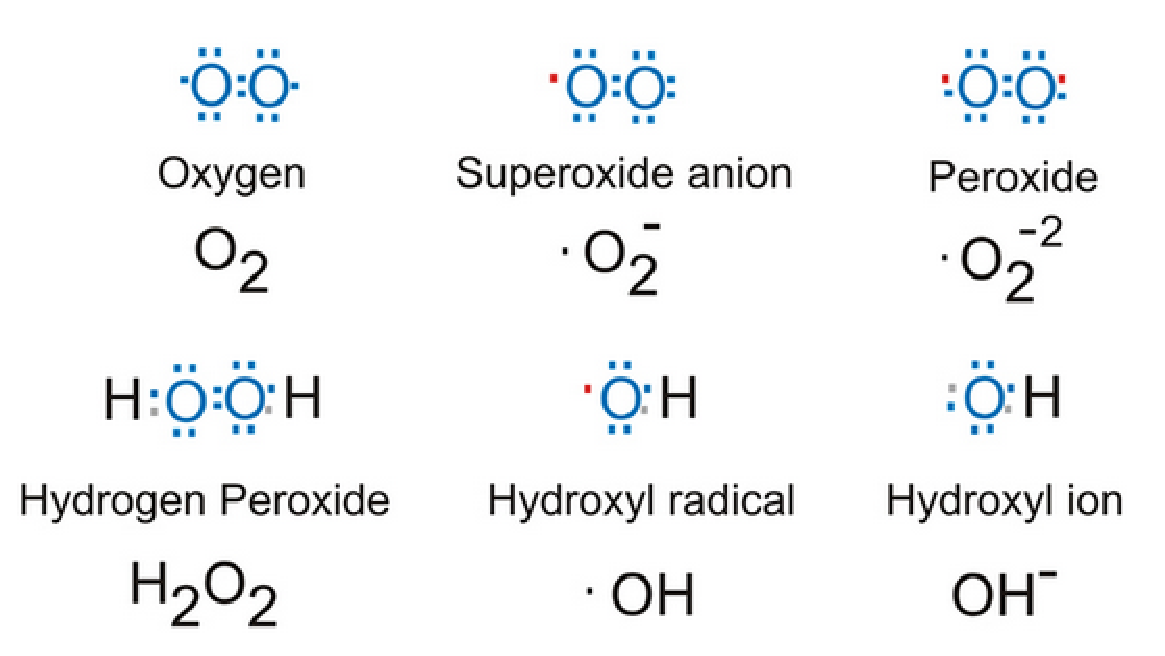
\includegraphics[height=5cm,
    angle=0]{./images/ROS.eps}}
\caption{Common reactive oxygen species}
\label{fig:ROS}
\end{figure}


Reactive oxygen species (ROS) is a normal byproduct of the normal oxidative
phosphorylation process (Sect.\ref{sec:oxidative-phosphorylation}).
\begin{itemize}
  \item found in Complex I - Sect.\ref{sec:complex-I-mito}
\end{itemize}

However, the
more-than-needed high level of ROS can damage the cell structures, e.g. damage
ADN, oxidize amino acids of proteins\ldots To fight against this, cell defends
itself using different mechanisms, e.g. superoxide dismutases,
peroxiredoxins\ldots Vital molecules can also help cell antioxidants like
vitamin C, vitamin E, uric acid.

\subsection{electron acceptors (i.e. oxidizers): NAD+/NADP+}
\label{sec:electron-acceptor}

In cells, common electron acceptors being \ce{NAD^+} (Sect.\ref{sec:NAD+}),
NADP+ (Sect.\ref{sec:NADP+}) or FAD. They are considered as co-enzyme
(Sect.\ref{sec:enzyme-coenzyme}) for dehydrogenase (Sect.\ref{sec:dehydrogenase}) in a redox reaction
(Sect.\ref{sec:redox_reaction-biology}).
They receives electrons via the enzyme dehydrogenase
(Sect.\ref{sec:dehydrogenase}).

Once receiving the electrons, the electron carriers are reduced in this process
and considered oxidizers of the substrate.



{\bf NADP+}: with the same capability like \ce{NAD^+}, but both involve into very
different chemical reactions. NADP+ involves in anabolic reactions; with the
reation occurs in the reverse direction (ratio of NADP+ to NADPH in the cell is
kept rather low, so that NADPH is readily available as a reducing agent)
\begin{equation}
\ce{NADP+ + 2H+ + 2e- <-> NADPH + H+}
\end{equation}



\subsection{-- Beta oxidation}
\label{sec:beta-oxidation}

\textcolor{red}{\bf $\beta$-oxidation}: The process that break-down
saturated fatty acid molecules
\begin{itemize}
  \item in the cytosol (in the case of
prokaryotes) and

  \item inside the matrix of the mitochondria (in the case of eukaryotes) to
  generate acetyl-CoA (Sect.\ref{sec:Acetyl-CoA}).

  \item in {\it peroxisome} (Sect.\ref{sec:peroxisome}) -  a type of organelle
  known as a microbody, found in virtually all eukaryotic cells.
\end{itemize}

Fatty acid $\beta$-oxidation is a multistep process by which fatty acyl-CoA
esters are stepwise shortened between carbons 2 and 3, yielding as products: a
chain-shortened acyl-CoA - and-depending on the presence of a 2-methyl group in
the substrate-acetyl-CoA or propionyl-CoA. \textcolor{red}{4 consecutive
reactions}
\begin{verbatim}

// desaturation of the bond between C2 and C3
// which is catalyzed by
//    1. FAD-dependent acyl-CoA oxidases (ACOXs) in peroxisomes
// .. 2. FAD-dependent acyl-CoA dehydrogenases (ACADs) in mitochondria
fatty acids   --[ACOX]-->


fatty acids   --[ACAD]-->


// hydration of the formed 2-enoyl-CoA

// dehydrogenation of 3-hydroxyacyl-CoA

// thiolytic cleavage of 3-oxoacyl-CoA

\end{verbatim}

The Krebs cycle and the electron transport chain metabolize {\bf triglycerides}
(stored fat) and carbohydrates (Sect.\ref{sec:carbohydrates}) to produce ATP.
The breakdown of triglycerides is called {\bf lipolysis}
(Sect.\ref{sec:lipolysis}). The byproducts of lipolysis are glycerol and free
fatty acids.

However, before free fatty acids can enter the Krebs cycle they must enter the a
catabolic process (Sect.\ref{sec:catabolic-reaction}) of {\bf beta oxidation}
where a series of chemical reactions downgrades them to Acetyl CoA and hydrogen.
The Acetyl CoA now enters the Krebs cycle and fat is metabolized just like
carbohydrates.




\section{Oxidative phosphorylation}

Sect.\ref{sec:oxidative-phosphorylation}

\section{tendency of reaction}


The direction of many cellular processes depends on 'redox state,'
(Sect.\ref{sec:redox-state}) based on mostly observational in that cells or
tissues are subjected to an oxidative or reductive stress and then the effects
are observed.

The tendency of the whole reaction to proceed can be calculated from reduction
potentials (Sect.\ref{sec:reduction-potential}) of half reactions, which have
been determined experimentally, using the formula.
\begin{equation}
\Delta E = (E_0 \text{ from reaction where e- are gained)} - (E_0 \text{ from
reaction where e- are released)}
\end{equation}
A positive $\Delta E_0$ tells you that the reaction will proceed in the
direction it is written.

\textcolor{red}{IMPORTANT}: The $\Delta E_0$ value is independent of the numbers
of electrons that are in the half reactions.

Example: The redox reaction in that cytochrome C molecules are oxidized in a
redox reaction where oxygen that we breathe is reduced:
\begin{equation}
\ce{4 cytochrome c_2+ + 4 H+ + O2 \rightarrow 4 cytochrome c_3+ + 2 H2O}
\end{equation}
which is divided into two half-reactions
\begin{equation}
\begin{split}
\ce{cytochrome c_3+ + e- \rightarrow cytochrome c_2+} \qquad; E_0 = 0.235 \text{
V} \\
\ce{O2 + 2 H+ + 2 e- \rightarrow H2O} \qquad; E_0 = 0.815 \text{ V}
\end{split}
\end{equation}
Now, the two half-reactions both has positive reduction potential $E_0$, which
means both have the tendency to gain electrons. However,
Reaction (2) has the higher E0, and is thus more likely to gain electrons; and
thus reaction (1) will be forced (by reaction (2)) backwards, becoming an
oxidation reaction.

So, in order to "add" the two half reactions together to get the whole reaction,
we will have to reverse half reaction (1):
\begin{equation}
\ce{cytochrome c_2+ \rightarrow cytochrome c_3+ + e- } \qquad; E_0 = -0.235
\text{ V}
\end{equation}
Finally, we will have to multiply the above reaction [reverse of (1)] by 4, and
reaction (2) by 2, to get the final reaction. And to calculate $\Delta E_0$, the
reduction potential $E_0$ on each half-reaction is not multiplied by the factors
as $\Delta E_0$ is independent of the numbers of electrons that are in the half
reactions.
\begin{equation}
\Delta E_0	= (0.815 V) - |(- 0.235 V)| = 0.580
\end{equation}


\section{redox state}
\label{sec:redox-state}

The quantitatively definition of {\bf redox state} is not well defined in many
studies, and thus has been defined by Schafer and Buetner (2001).

\begin{enumerate}
  \item (historically) described as the ratio of the interconvertible oxidized
  and reduced form of a specific redox couple.

Example: redox state of \ce{NAD^+}/NADH couple in a cell to be
[free \ce{NAD+}]/[free NADH] (Sir Hans Crebs)

  \item (current use) not only to describe the state of a particular redox
  pair; but also more generally describe the redox environment of a cell
  (Sect.\ref{sec:redox-environment}). In such cases, Schafer-Buetiner (2001)
  suggested to call this {\bf redox environment}.

This more general use of the term redox state is not very well
defined and differs considerably from historical uses.

\end{enumerate}

The redox state of the mitochondria is a sensitive indicator of the
intracellular metabolic state and can be used to evaluate the cellular energy
status.

\subsection{redox environment (new usage of redox state)}
\label{sec:redox-environment}

The redox environment is a new name and usage for redox state
(Sect.\ref{sec:redox-state}), as suggested by Schafer-Buetiner (2001).

The redox environment of a linked set of redox couples as found in a biological
fluid, organelle, cell, or tissue is the summation of (across all redox couples)
the products of the reduction potential $E_i$
(Sect.\ref{sec:reduction-potential}) and reducing capacity of the linked redox
couples present, i.e. [reduced species] concentration (Schafer-Buetiner, 2001).

\begin{equation}
\text{redox environment} = \sum\limits_{i=1}^{n(\text{couple})} E_i \times
[\text{reduced species}]_i
\end{equation}
with $E_i$ is half-cell reduction potential for a given redox pair/couple
(Set.\ref{sec:reduction-potential}); and [reduced species]$_i$ is the concentration of
the reduced species in that redox pair.
Nernst equation can be a tool to provide quantitative estimates of redox
state (Sect.\ref{sec:nernst-equation}).

\subsection{oxidation potential ??}


We know that a redox reaction consists of both a reduction and an oxidation.
Shouldn't there be such a thing as an "oxidation potential," too?

ANSWER: We don't need, as it turns out, you can tell how likely a compound is to
be oxidized from the reduction potential. Since, a high (large positive)
reduction potential (Sect.\ref{sec:reduction-potential}) means a high tendency
to be reduced, it must follow that a lower reduction potential must mean that a
compound is less likely to be reduced.

If a compound is less likely to be reduced, it is more likely to be oxidized.

\subsection{reduction potential E (redox potential)}
\label{sec:reduction-potential}
\label{sec:redox-potential}

The {\bf reduction potential}
(pE, $\varepsilon$, $E_h$) measure the tendency of a chemical species to gain
electrons (i.e. be reduced). The reduction potential is the tendency of a
compound to be reduced.
\begin{enumerate}
  \item the more positive pE, the greater tendency to gain electrons or to be
  reduced
\end{enumerate}

The standard reduction potential is defined relative to a standard hydrogen
electrode (SHE) reference electrode, which is arbitrarily given a potential of
0.00 V.The standard reduction potential is defined relative to a standard
hydrogen electrode (SHE) reference electrode, which is arbitrarily given a
potential of 0.00 V.


The reduction potential is experimentally determined for the oxidation and
reduction half reactions, and is called $E_0$.
To remember the relationship of E0 and oxidation and reduction, consider $E_0$
as how much a compound wants to get reduced (it has a lot of potential for
reduction). NOTE: RIG = reduction is a gain of electron.
\begin{itemize}

  \item  \textcolor{red}{the larger (more positive) the E0, the more likely the
  compound in the half reaction is to gain electrons (be reduced)}.

  \item the E0 values can be looked up in tables, and are always given for
  reduction half-reactions (reactions gaining electrons).

Example:
\begin{equation}
\ce{S + 2H^+ + e^- -> H2S } \qquad; E_0 = -0.23 \text{ V}
\end{equation}
\end{itemize}

{\bf Reduction potential} $E$ can be thought of as a voltage and reducing
capacity would be total charge stored, that is, number of electrons available or
the concentration of reduced species [reduced species]$_i$.

Thus, with the Nernst equation (Sect.\ref{sec:nernst-equation}), the reduction
potential $E$ between two redox couples (electrodes) in an electrochemical cell
can be estimated
\begin{itemize}
  \item half-cell reduction potential E$_{\text{hc}}$

  \item
\end{itemize}




\subsection{redox couple}
\label{sec:redox-couple}

There are many redox couples in a cell that work together to maintain the redox
environment (Sect.\ref{sec:redox-environment}).

\begin{enumerate}
  \item  GSSG/2GSH couple is the most abundant redox couple in a cell

  \item \ce{NAD^+}/NADH couple: Sect.\ref{sec:NAD+-NADH-couple}

  \item NADP+/NADPH couple:
\end{enumerate}

\subsection{-- \ce{NAD^+}/NADH couple (or ratio)}
\label{sec:NAD+-NADH-couple}
\label{sec:NAD+-NADH-ratio}

Nicotinamide adenine dinucleotide (NAD) - Sect.\ref{sec:NAD}


\ce{NAD^+} - Sect.\ref{sec:NAD+} and NADH (Sect.\ref{sec:NADH}).
The ratio \ce{NAD^+}/NADH is typically high in cells. To make the reaction moving in
the forward direction easily, the ratio of \ce{NAD^+} to NADH is kept very high in the
cell, keeping it readily available to act as an oxidizing agent
(Sect.\ref{sec:glycolysis}).

NAD = nicotinamide adenine dinucleotide, contributes to the creation of proton
gradients to drive the synthesis of ATP.

A significant decrease in \ce{O2} supply to the brain will cause a decrease in
ATP levels along with a rise in NADH. It is followed by the inhibition of the active
transport mechanisms (such as Na+-K+- ATPase) and elevation of extracellular K+
levels, until the normal energy supply is restored.


\subsection{important biological redox couples that play a role in determining
the cellular redox environment}



\section{Reducing equivalents}
\label{sec:reducing-equivalent}

In biochemistry, the term {\bf reducing equivalent} refers to any
chemical species which transfer the equivalent of one electron in redox
reactions (Sect.\ref{sec:redox-reaction}).

Examples:
\begin{itemize}
  \item a lone electron, e.g. reaction involving metal ions
  \item a hydrogen atom (with a proton and an electron)
  \item a hydrogen ion (:\ce{H^-}, which carries two electrons)
  \item NADH - Sect.\ref{sec:NADH}
  \item \ce{FADH2}
\end{itemize}


\section{Coenzyme (cofactor)}
\label{sec:enzyme-coenzyme}
\label{sec:co-enzyme}
\label{sec:apo-enzyme}
\label{sec:holo-enzyme}
\label{sec:cofactor}

Cellular activities need energies - ATP. To generate ATP, many reactions require
strict conditions to occur, e.g. like high temperatures, extreme pH values, and
high concentration of reactants.

Food molecule like glucose is stable at body temperature. The question
is \textcolor{red}{how can the body break the glucose and convert to the
ATP under cellular normal condition?}  The answer is with the help of the
enzymes (Sect.\ref{sec:enzyme}), and also {\bf coenzymes}.

Coenzymes (aka cosubstrates) are small (organic) molecules, i.e. not a protein.
They cannot by themselves catalyze a reaction but they can help enzymes to do so.
Coenzymes bind with the protein molecule (apoenzyme) to form the active enzyme
(holoenzyme).  The apoenzyme is the lock, and the coenzyme is the key.

\begin{mdframed}

A {\bf cofactor} are organic or inorganic molecules, e.g.
\begin{itemize}
  \item metallic inorganic ions, or

  \item a non-protein organic compound known as {\bf coenzymes }
\end{itemize}
that is required for an enzyme's biological activity to happen.
\end{mdframed}


Coenzymes is mostly derived from vitamins and other organic essential nutrients
in small amounts.  Coenzymes loosely or tightly bound to the enzyme and directly
participate in the reaction. 
\begin{itemize}
  \item  Some coenzymes function by ferrying electrons or negative charges to
  enhance a reaction. 

Vitamins B-2, B-3 and C are all precursors of
electron-carrying coenzymes
\begin{enumerate}
  
  \item  Vitamin B-2 (or riboflavin) is the precursor for the flavin coenzymes
flavin mononucleotide (or {\bf FMN}), and flavin adenine dinucleotide ({\bf
FAD} - Sect.\ref{sec:FAD}). Their main function is to accept and store
electrons within proteins.

  \item Vitamin B-3, on the other hand, is the precursor for the nicotinamide
  coenzymes, nicotinamide adenine dinucleotide, or NAD (Sect.\ref{sec:NAD}), and
  nicotinamide adenine dinucleotide 2'-phosphate, or NADP - Sect.\ref{sec:NADP},
  which carry electrons between different proteins.

NOTE: NAD is the first organic cofactor to be discovered, which was identified
by Arthur Harden and William Youndin 1906.
  
  \item  Vitamin C, or ascorbic acid, acts as an electron donor, changing in the
  process to dehydroascorbic acid.
  
  This reaction is important for the production of bile acid and the break down
  of tyrosine.
\end{enumerate}

  \item Vitamin B-12-derived Coenzymes
  
Methylcobalamin and 5'-deoxyadenosylcobalamin are two coenzymes formed from
vitamin B-12 or cobalamin. Methylcobalamin is required for the production of
methionine from homocysteine, while 5'-deoxyadenosylcobalamin has the role of
changing the molecular arrangement of the metabolic product of some amino acids.

  \item Coenzyme from Vitamin B-5

Vitamin B-5, or pantothenic acid, is used to make coenzyme A, often termed CoA
(Sect.\ref{sec:coenzyme-A}).
This has a free sulfur-containing group that can attach and move carbon
compounds. Reactions that utilize pantothenic acid derived coenzymes include the
production of fatty acids.   

  \item Metabolite Coenzymes

The most common metabolite coenzyme is adenosine triphosphate, or ATP. There are
four reactions involving ATP, each involving the movement of a part of the ATP
molecule. An adenosine monophospate or AMP group is transferred in the reaction
that produces 5-phosphoribosyl-1-pyrophosphate, while an adenosine diphosphate
or ADP group is transferred when glucose-6-phosphate is made. Two reactions
require the transfer of a phosphoryl group, one to facilitate the production of
S-adenosyle methionine from methionine, and the other, the production of
glutamine synthetase-O-AMP.
 
\end{itemize}
"High energy electrons" refer to the reduced forms of these coenzymes.

\subsection{NADP: oxidized form \ce{NADP^+}, and reduced form NADPH}
\label{sec:NADP}
\label{sec:NADP+}
\label{sec:NADPH}

Nicotinamide adenine dinucleotide phosphate (\ce{NADP}), or in older notation,
TPN (triphosphopyridine nucleotide), is a cofactor that can exist in two forms
\begin{enumerate}
  \item oxidized form \ce{NADP^+}
  
  \item reduced form \ce{NADPH}
\end{enumerate}

NADP, or to be precise \ce{NADPH}, involves in anabolic
reactions, such as lipid and nucleic acid synthesis, as these reactions require
NADPH as a reducing agent. 

Another energized biomolecule is {\it nicotinamide adenine dinucleotide
phosphate} (NADPH) used in anabolic reactions (e.g. in lipids or nucleic acids
synthesis).  

% NADPH is the reduced form of NADP+, i.e. NADP+ is the oxidized form
% of
% NADPH\footnote{\url{http://web.virginia.edu/Heidi/chapter1/Flash/figure1_3_nadph.html}}.


\subsection{NAD: oxidized form \ce{NAD^+}, reduced form NADH}
\label{sec:NAD}
\label{sec:Nicotinamide-adenine-dinucleotide}
%\subsection{\ce{NAD^+}: coenzyme with high energy electron}
\label{sec:NAD+}

Nicotinamide adenine dinucleotide (NAD) is one of the most important coenzymes
in the cell (Sect.\ref{sec:co-enzyme}) with its role in redox reactions.  NAD is
the first organic cofactor to be discovered, which was identified by Arthur
Harden and William Youndin 1906.

NAD exists in 2 forms:
\begin{enumerate}
  \item oxidized form as \ce{NAD^+}

{\bf \ce{NAD^+}} is a di-nucleotide, i.e. containing 2 nucleotides; and involve in
catabolic pathways
\begin{itemize}
  \item one nucleotide contains {\bf adenine group}
  \item .. contains {\bf nicotidamine group}
\end{itemize}
In order to reduce this molecule, a hydrogen and two electrons must be added to
the 6-carbon ring of nicotinamide.
  
NAD+ upon lossing one electrons (e-) turns into NADH.

  
  \item NAD (its base form)
  
  \item reduced form as \ce{NADH}, i.e. with adding electron into \ce{NAD^+} at
  nitrogen atom, and one hydrogen atom (1 electron + 1 proton) at the upper
  position of nicotinamide ring.
  

\begin{mdframed}
Although \ce{NAD^+} is written with a superscript plus sign because of the formal
charge on a particular nitrogen atom, at physiological pH for the most part it
is actually a singly charged anion (charge of minus 1), while NADH is a doubly
charged anion.
\begin{equation}
\ce{NAD+ + 2H+ + 2e- <-> NADH + H+}
\end{equation}


NADH is a reduced form of \ce{NAD^+}, meaning \ce{NAD^+} gains electrons to become
NADH (oxidation is losing electrons).
\begin{equation}
\begin{split}
&\ce{NADH + H+ + 1/2 O2 -> NAD+ + H2O}  \\
&\ce{NAD+ + 2e- + H+ -> NADH } \qquad  E^o = -0.315 V \\
&\ce{1/2O2 + 2e- + 2H+ -> H2O} \qquad E^o = +0.816 V \\
&\Delta E^o = (+0.816) - (-0.315) = 1.136 V \\
&\Delta G^{\circ} = - n \times F \times \Delta E^o = -219 \text{ kJ/mol} \\
&\ce{ADP + Pi -> ATP } \qquad \Delta G^{\circ} = +30.5 \text{ kJ/mol}
\end{split}
\end{equation}

So, if we can convert all 'free energy' (i.e. 219 kJ/mol) into synthesizing ATP
(from ADP, Pi; which require 30.5 kJ/mol); then we can create
\begin{equation}
219/30.5 \approx 7.2 \qquad \text{ATP molecules}
\end{equation}


\end{mdframed}

  
\end{enumerate}
% Although \ce{NAD^+} is written with a superscript plus sign because of the formal
% charge on a particular nitrogen atom, at physiological pH for the most part it
% is actually a singly charged anion (charge of minus 1), while NADH is a doubly
% charged anion.

There was such a huge variety of processes requiring NAD+. 
\begin{enumerate}
  \item  The main (and classical) role of \ce{NAD^+} in metabolism is the transfer of electrons from
one it to another, and becoming NADH. Thus the ratio \ce{NAD^+}/NADH is very important
in controling the direction of the reaction (Sect.\ref{sec:NAD+-NADH-ratio}).

  \item Apart from its role in redox reactions, NAD+ (but not NADH) has been
  recognized
its role in signaling. In recent years, NAD+ has also been recognized
as an extracellular signaling molecule involved in cell-to-cell communication.
NAD+ is released from neurons in blood vessels.
It has been studied for its potential use in the therapy of neurodegenerative
diseases such as Alzheimer's and Parkinson disease.
\end{enumerate}


\begin{mdframed}

NAD and the closely related NADP
are the two most abundant cofactors in eukaryotic cell.

NAD coenzyme acts as a hydrogen acceptor in oxidation-reduction
reactions (Sect.\ref{sec:redox-reaction}).

\end{mdframed} 

The major question is
what does it do to human health, given that levels of NAD+ decline with age?

\begin{enumerate}
  
   \item biosynthetic enzymes decrease in their expression. Consequently, less of
the proteins are present that make NAD+, which means you have less NAD+
synthesis, which would explain why it goes down
  
  \item an alternative could be that you increase consumption. It could well be
  you need more of these signaling processes to cope.

Example: PARPs are involved in DNA repair. If you need to repair more DNA damage, you would consume more NAD+
\end{enumerate}

\label{sec:PARP}
PARPs: Stands for poly (ADP-ribose) polymerase. PARPs are a family of 17 proteins that require NAD+ to function.
The field is working to better understand how PARPs function in normal biology.

\label{sec:sirtuins}
Sirtuins: A family of seven proteins that help maintain homeostasis in the cell and also play a role in aging. 
Sirtuins require NAD+ to function.

Reference: \url{https://endpoints.elysiumhealth.com/nad-conference-interview-mathias-ziegler-ed874b25b0d1}

\subsection{FMN (Flavine MonoNucleotide)}
\label{sec:FMN-coenzyme}

Flavin coenzymes {\bf flavin mononucleotide} (or {\bf FMN})'s main function is
to accept and store electrons within proteins. FMN is also part of some
flavoprotein (Sect.\ref{sec:flavoprotein})

\subsection{FAD (Flavin Adenine Dinucleotide)}
\label{sec:FAD}

{\bf FAD}, as a redox cofactor, its main function is to accept and store
electrons within proteins. It is also part of some flavoprotein
(Sect.\ref{sec:flavoprotein})

FAD can exist in 4 different forms
\begin{enumerate}

  \item flavin-N(5)-oxide, i.e. the superoxidized form of FAD, and is
  yellow-orange color
  
  \item FAD  (itself or fully oxidized form): is yellow color 

FAD accepts 1 protons (\ce{H+}) to become quinone.

FAD accepts 1  electrons, and 2 protons (\ce{H+}) to become semiquinone.

FAD accepts 2 electrons, and 3 protons (but also release one proton, so it
needs only 2 in overall) to become hydroquinone (FADH2).

\begin{equation}
\ce{FAD + 2H+ + 2e- <-> FADH2}
\end{equation}
NOTE: partial form
\begin{equation}
\begin{split}
\ce{FAD + 2H+ + 2e- <-> FADH + H+} \\
\ce{FADH + H+ <-> FADH2}
\end{split}
\end{equation}

  \item quinone, i.e. the fully oxidized form of FAD

Quinone accepts 2 electrons, and 2 protons to become hydroquinone (FADH2).
  
  \item semiquinone, i.e. \ce{FADH^{·}} (or half-reduced form) is either blue or
  red based on the pH
  
  \ce{FADH^{·}} can be formed by either reduction of FAD or oxidation of FADH2
  by accepting or donating one electron and one proton, respectively
  
  \item hydroquinone (FADH2) - the fully reduced form - is colorless

FADH2, upon lossing of 1 H+ and 1 e−, to form \ce{FADH^{.}} 

%Quinone accepts 2 electrons, and 2 protons to become FADH2.  
\end{enumerate}

NOTE:  FAD is an aromatic ring system, whereas FADH2 is not. This means that
FADH2 is significantly higher in energy,

unlike \ce{NAD^+}/NADP+, FAD takes two protons; and thus FAD is often
involved when a double bond is formed in the newly oxidized substrate.

\url{https://en.wikipedia.org/wiki/Flavin_adenine_dinucleotide}

\subsection{Coenzyme Q10: Ubiquinol (QH2), ubiquinone (Q)}
\label{sec:ubiquinol}
\label{sec:coenzyme-Q10}

Coenzyme Q10 (CoQ10 - Sect.\ref{sec:co-enzyme}) is a fat-soluble nutrient produced
naturally by our bodies.

CoQ10 exists in three redox states, fully oxidized (ubiquinone), partially
reduced (semiquinone or ubisemiquinone), and fully reduced form (ubiquinol).

Ubiquinol is an electron-rich (reduced) form of coenzyme Q10.




\section{NADH and \ce{FADH_2}}
\label{sec:NADH-FADH2}
\label{sec:NADH}
\label{sec:FADH2}

The two reducing agents (Sect.\ref{sec:reductant}), NADH and \ce{FADH_2} are
utilized by ETC (Sect.\ref{sec:ETC}) to produce ATP.

\begin{table}[hbt]
\begin{center}
    \begin{tabular}{p{6cm}|p{6cm}}
        \hline
         NADH &  \ce{FADH2} \\
        \hline \hline
{\bf Nicotinamide Adenine Di-nucleotide} &  {\bf Flavin adenine di-nucleotide} \\
\multicolumn{2}{p{12cm}}{more NADH is created and used than \ce{FADH2}
in the process of creating ATP. {\it glycolysis + intermediate steps + Krebs's
cycle creates 10 NADH molecules and 2 \ce{FADH2} molecules are produced}  } \\
        \hline
 \multicolumn{2}{p{12cm}}{both are redox cofactor, or reduced enzymes} \\
created during Krebs cycle and/or during glycolysis
and/or made in the body using vitamin B3 (also known as niacin, or nicotinamide)
as the starting point &  created during Krebs cycle
(Sect.\ref{sec:krebs-cycle}) \\
        \hline
$\ce{NAD^+ + 2H -> NADH + H^+}$ & $\ce{FAD -> FADH_2}$ \\
        \hline
{\tiny$\ce{NADH + H^+ + 1/2 O2 -> NAD^+ + H2O}$} & {\tiny$\ce{FADH_2 + 1/2 O2
-> FAD + H2O}$}
\\
$\Delta G^\circ = -52.6$ (kcal/mol) & $\Delta G^\circ = -43.4$ (kcal/mol)
\\
\multicolumn{2}{p{12cm}}{Total free energy changes: $\Delta G^\circ$ =
10*(-52.6) + 2*(-43.4) = -680 (kcal/mol)}
    \end{tabular}
\end{center}
\caption{Compare NADH and \ce{FADH2}}
\label{tab:comparison-NADH-FADH2}
\end{table}

%TUANTUAN
an important {\it pyridine
nucleotide} that functions as an oxidative cofactor in eukaryotic cells. NADH
is a major carrier of $\ce{H}$ and e$^{-}$; thus plays a key role in the
production of energy through redox reactions (Sect.\ref{sec:complex-I-mito}).

\begin{itemize}
  \item NADH is equivalent to 2.5 ATP molecules (maximum 3).

  NADH will be oxidized (donate its electrons) to drive ATP synthesis in a type
  of process called oxidative phosphorylation.

  \item \ce{FADH_2} is equivalent to 1.5 ATP molecules (generated in oxidative
  phosphorylation)

   \ce{FADH_2}, though not directly generate ATP, facilitates transfer of electrons to
   coenzyme Q, which is the final electron acceptor of the reaction catalyzed by
   the Succinate:ubiquinone oxidoreductase complex, also acting as an
   intermediate in the electron transport chain
\end{itemize}

\subsection{NADH redox state}
\label{sec:NADH-redox-state}

One significant parameter to be monitored is the NADH redox state.
The principle of NADH monitoring from the brain surface is using {\bf NADH
fluorescence}

\begin{itemize}
  
  \item   Excitation light (366 nm) passes from the fluorometer to the brain via
  a bundle of optical fibers made of quartz.
  
  \item   The light emitted by NADH (450 nm), along with the reflected light at
  the excitation wavelength, is transferred to the fluorometer via another
  bundle of fibers.
  
  \item The changes in the reflected light correlate with the changes in tissue
  blood volume and also serve to correct for hemodynamic artifacts appearing
  in NADH measurements (for details see (Mayevsky, 1984) 

Mayevsky and collaborators (Mayevsky and Chance, 1974; Friedli et al., 1982;
Mayevsky, 1983b; Mayevsky and Weiss, 1991; Mayevsky et al., 1998) measured in
vivo the oxidation–reduction state of intramitochondrial pyridine nucleotides by
a multichannel fluorometer-reflectometer. This approach permitted (Kraut et al.,
2003) to measure the changes in the mitochondrial redox status (O2 balance) in
four different organs simultaneously (brain, liver, kidney, and testis) in the
same animal.
  
  \item The changes in fluorescence and reflectance signals are calculated
  relatively to the calibrated signals under normoxic conditions.
  
  This type of calibration is not absolutely exact, yet it has provided reliable
  and reproducible results in different animals and at different laboratories.
    
  \item  
\end{itemize}



Monitoring of brain energy metabolism, using fiber optic surface fluorome-
try/reflectometry, has been described in many publications (Mayevsky, 1984,
1993; Mayevsky et al., 1998; Meilin et al., 1999).

NADH levels due to pathological conditions, such as anoxia, hypoxia, and ischemia.

Conditions that activate brain metabolism, such as spreading depression and/or
convulsions, decreased the level of NADH in brain tissue, i.e., NADH was
oxidized to NAD (Mayevsky and Chance, 1975; Mayevsky, 1983a; Mayevsky and
Sclarsky, 1983).


\section{ATP - the most-commonly used free-energy currency (molcule of energy
supply)}
%\label{sec:introduction}
\label{sec:ATP-overview}
\label{sec:free-energy-currency}


Like any transaction or exchange needs money to facilitate such activity, every
activity needs energy. A car gets free energy from petrol oxidization; it does
not use petrol directly as the engine will burn the gas to create the thermal
energy for the piston to move the car. Petrol is the "nutrients" of cars.

The same as in life, an organism eats food, but it cannot use food directly. The
digestion system will break down the food into small molecules (sugar, amino
acids, lipids...) to provide components for forming new biomolecules. In
addition, it also needs to convert the food to a type of chemical compound that
can release the energy that every cellular's process can use
(Sect.\ref{sec:high-energy-compound}).

In this section, we discuss one important high-energy compound - a nucleotide
called {\bf adenosine triphosphate} (ATP) - Sect.\ref{sec:ATP-molecule}.
ATP is the most important "free-energy-currency" molecule in living organisms.

Although ATP is the most commonly used free-energy currency, any of these
phosphorylated molecules could, in theory, be used as free-energy currency.
Here, we rank them  in order of their efficiency (i.e., the amount of
nonspontaneous reactions enabled per phosphate removed from a molecule of
free-energy currency) from the most efficient to the least efficient.
\begin{enumerate}
  \item Acetyl phosphate: $\Delta G^\circ = -47.3 $ kJ/mol
  \item ATP (adenosine triphosphate): $\Delta G^\circ = -30.5$ kJ/mol
  \item Glucose-6P (Sect.\ref{sec:Glucose-6-phosphatase}):
  $\Delta G^\circ =-13.8 $ kJ/mol

  \item PEP (Phosphoenolpyruvate): $\Delta G^\circ = -61.9$ kJ/mol
  
  \item Phosphocreatine (Sect.\ref{sec:phosphocreatine}):
  $\Delta G^\circ =  -43.1$ kJ/mol
\end{enumerate}


NOTE: Whenever we write ATP, it means \ce{ATP^{4-}}; and whenever we write ADP,
it means \ce{ADP^{3-}}. The body's use of ATP as a free-energy currency is a
very effective strategy to cause vital nonspontaneous reactions to occur.

\begin{itemize}
  \item  The human heart contains ~ 0.7g of ATP and yet, it uses roughly 6kg ATP
  per day to maintain normal excitation-contraction cycle(Ingwall 2002)

  \item In a typical cell, an ATP molecule is used within a minute of its
  formation.  During strenuous exercise, the rate of utilization of ATP is even
  higher. Hence, the supply of ATP must be regenerated.
\end{itemize}

The released energy can be harnessed to power an energy-requiring
process (reaction) such as muscle contraction or protein synthesis. If
only the outermost phosphate group is removed, we obtained the
adenosine diphosphate (ADP) - Sect.\ref{sec:ADP}.

\textcolor{red}{The two reducing agents, NADH and \ce{FADH_2} are needed to
produce ATP} (Sect.\ref{sec:NADH}, Sect.\ref{sec:FADH2}).


\subsection{ATP molecule}
\label{sec:ATP-molecule}

\begin{framed}
  ATP is the universal energy source in life. It is the only form of
  energy that every cell can use directly. However, there can be other forms
  (Sect.\ref{sec:high-energy-compound}).
  \footnote{\url{http://answers.yahoo.com/question/index?qid=20061030225122AAmkucR}}

  Read Sect.\ref{sec:food} and
  Sect.\ref{sec:history-energy-metabolism-mechanism} to know that an organism
  get the energy from food which has difference classes of food molecule
  (carbohydrate, proteins, fats), which are broken into different energy
  substrates before they can be converted into ATP
  (Sect.\ref{sec:ATP-synthesis}).

%For the process of making ATP from food, read Chapter 12.

\end{framed}

ATP (adenosine triphosphate) is a nucleotide consisting of adenine, a
ribose and a triphosphate unit; with total molecular mass 507 Da.
There is 4 $e^{-}$ charges on ATP and 3 on ADP; therefore ATP is less stable.
Remember that when ADP is phosphorylated to ATP, entropy loss; and in the
reverse process, when ATP is hydrolized into ADP, energy is released.

\begin{figure}[hbt]
  \centerline{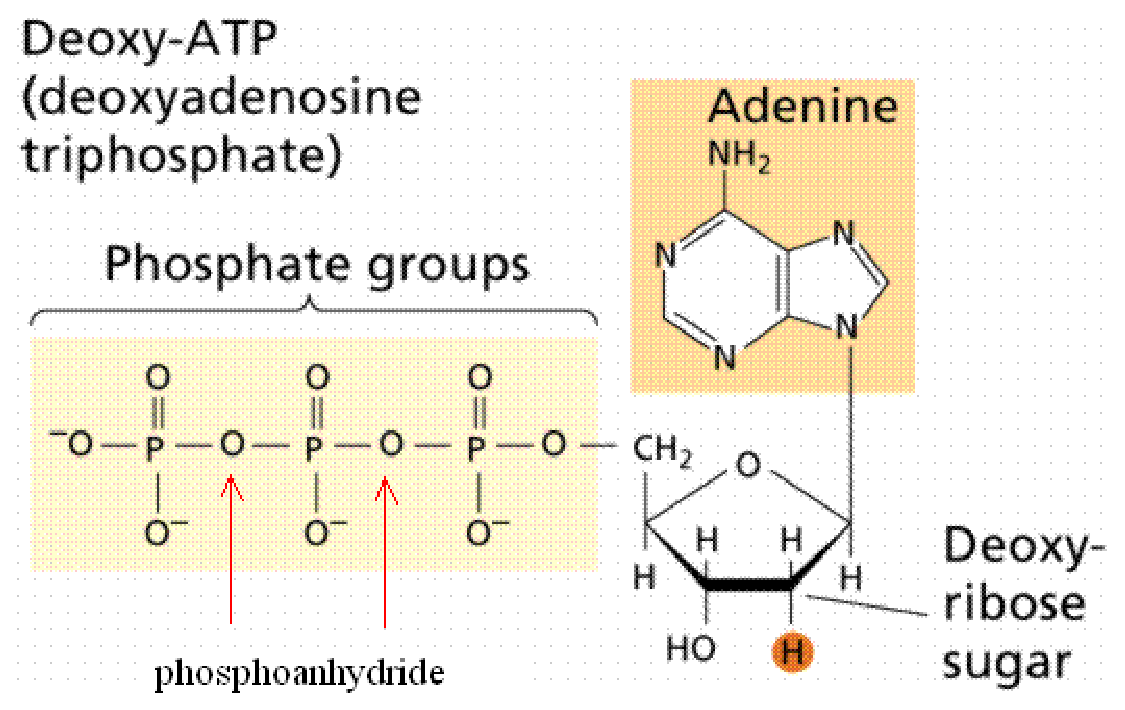
\includegraphics[height=4cm,
    angle=0]{./images/ATP.eps}}
\caption{ATP molecule}
\label{fig:ATP}
\end{figure}

\subsection{ATP hydrolysis}
\label{sec:ATP-hydrolysis}

The activation form of ATP is usually a complex with \ce{Mg^2+} or \ce{Mn^2+}. A
large amount of energy is released (i.e. $\Delta G^\circ < 0$) when ATP is
hyrolized into ADP or AMP.
\begin{equation}
  \label{eq:2}
  \begin{split}
    \ce{ATP + H2O <=> ADP + P_i } + \Delta G^{\circ}\;\;\; ; \Delta G^{\circ} = -7.3 kcal/mol\\
    \ce{ATP + H2O <=> AMP + PP_i} + \Delta G^{\circ} \;\;\; ; \Delta G^{\circ} = -10.9 kcal/mol
  \end{split}
\end{equation}
The value of $\Delta G^{\circ}$ varies with the milieu condition
(Sect.\ref{sec:Gibbs-free-energy}).

Under typical cellular concentrations, $\Delta G^{\circ} \approx -12 kcal/mol$
(equivalent to $-50 kJ/mol$). NOTE: $\Delta G^{\circ}<0$ means the process
release energy, because the system loss Gibbs free-energy.




\begin{figure}[hbt]
  \centerline{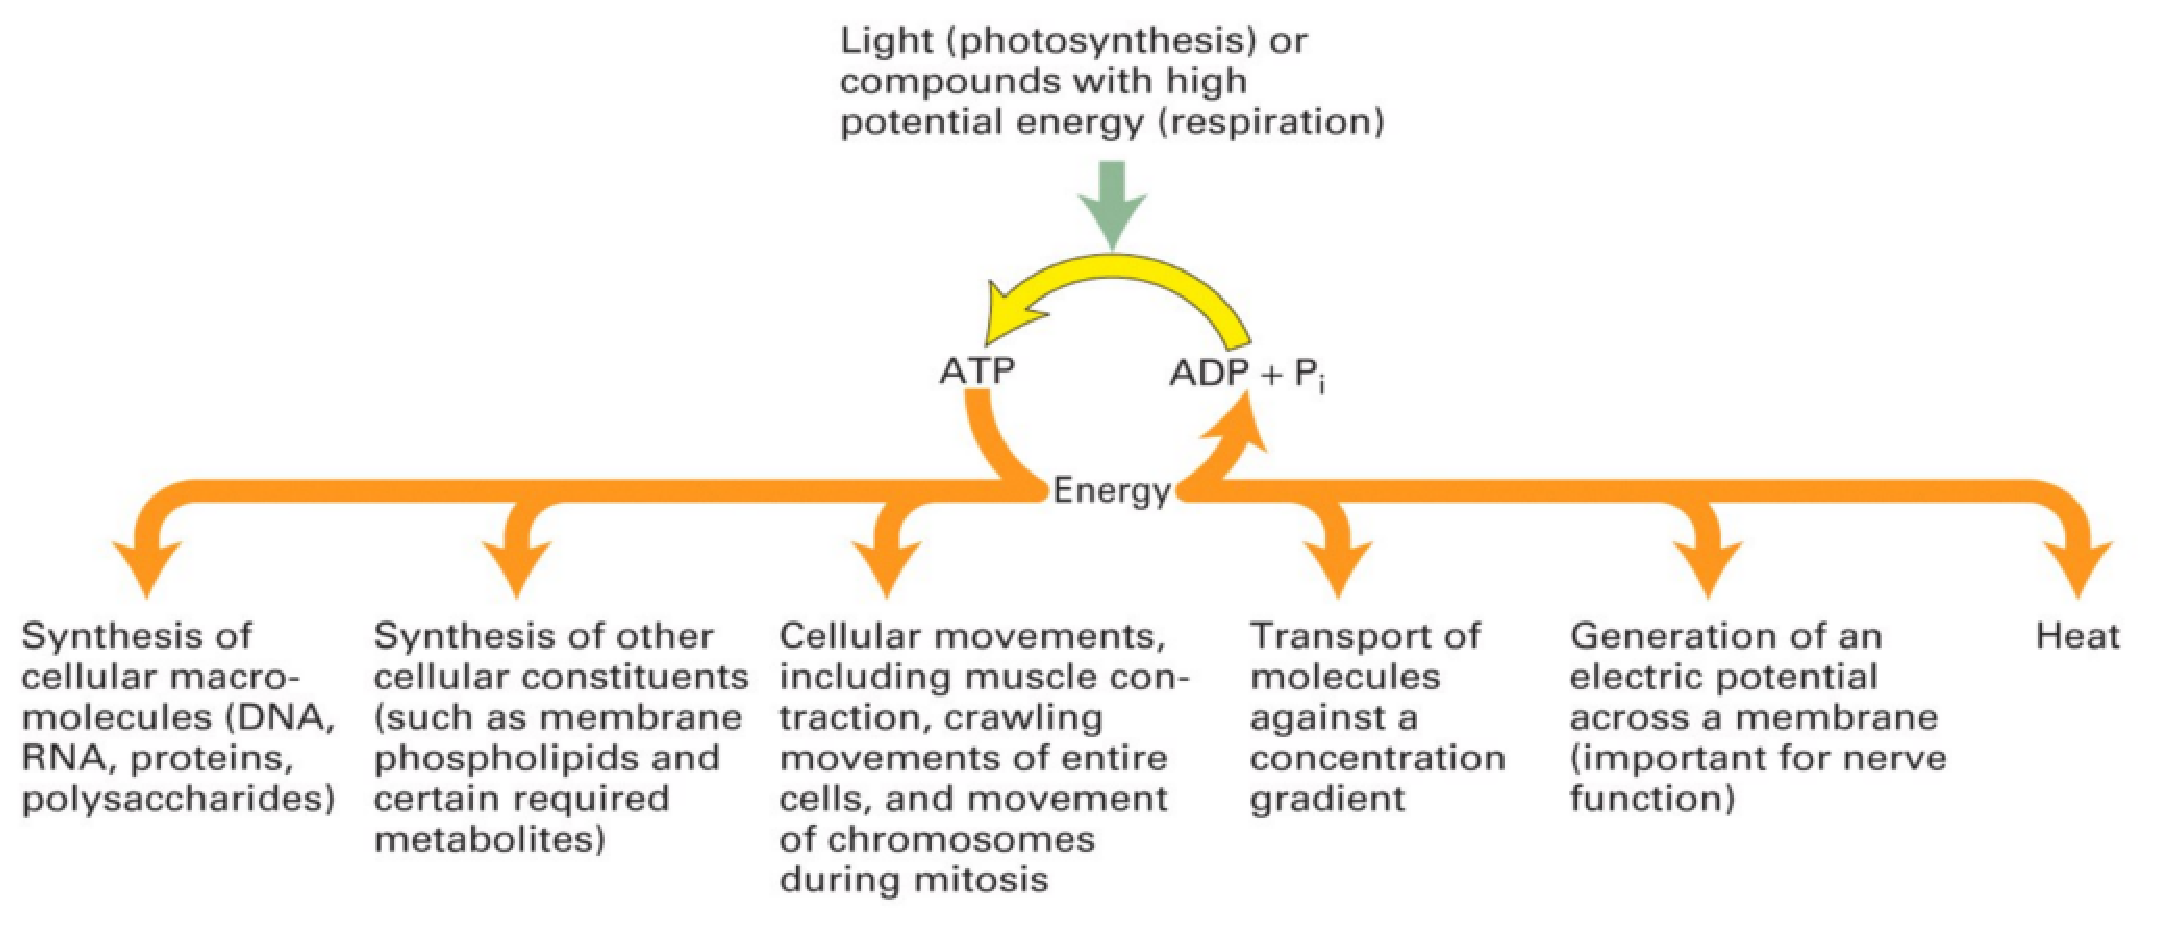
\includegraphics[height=5cm,
    angle=0]{./images/ATP_usage.eps}}
\caption{ATP usage}
\label{fig:atp}
\end{figure}



\begin{figure}[hbt]
  \centerline{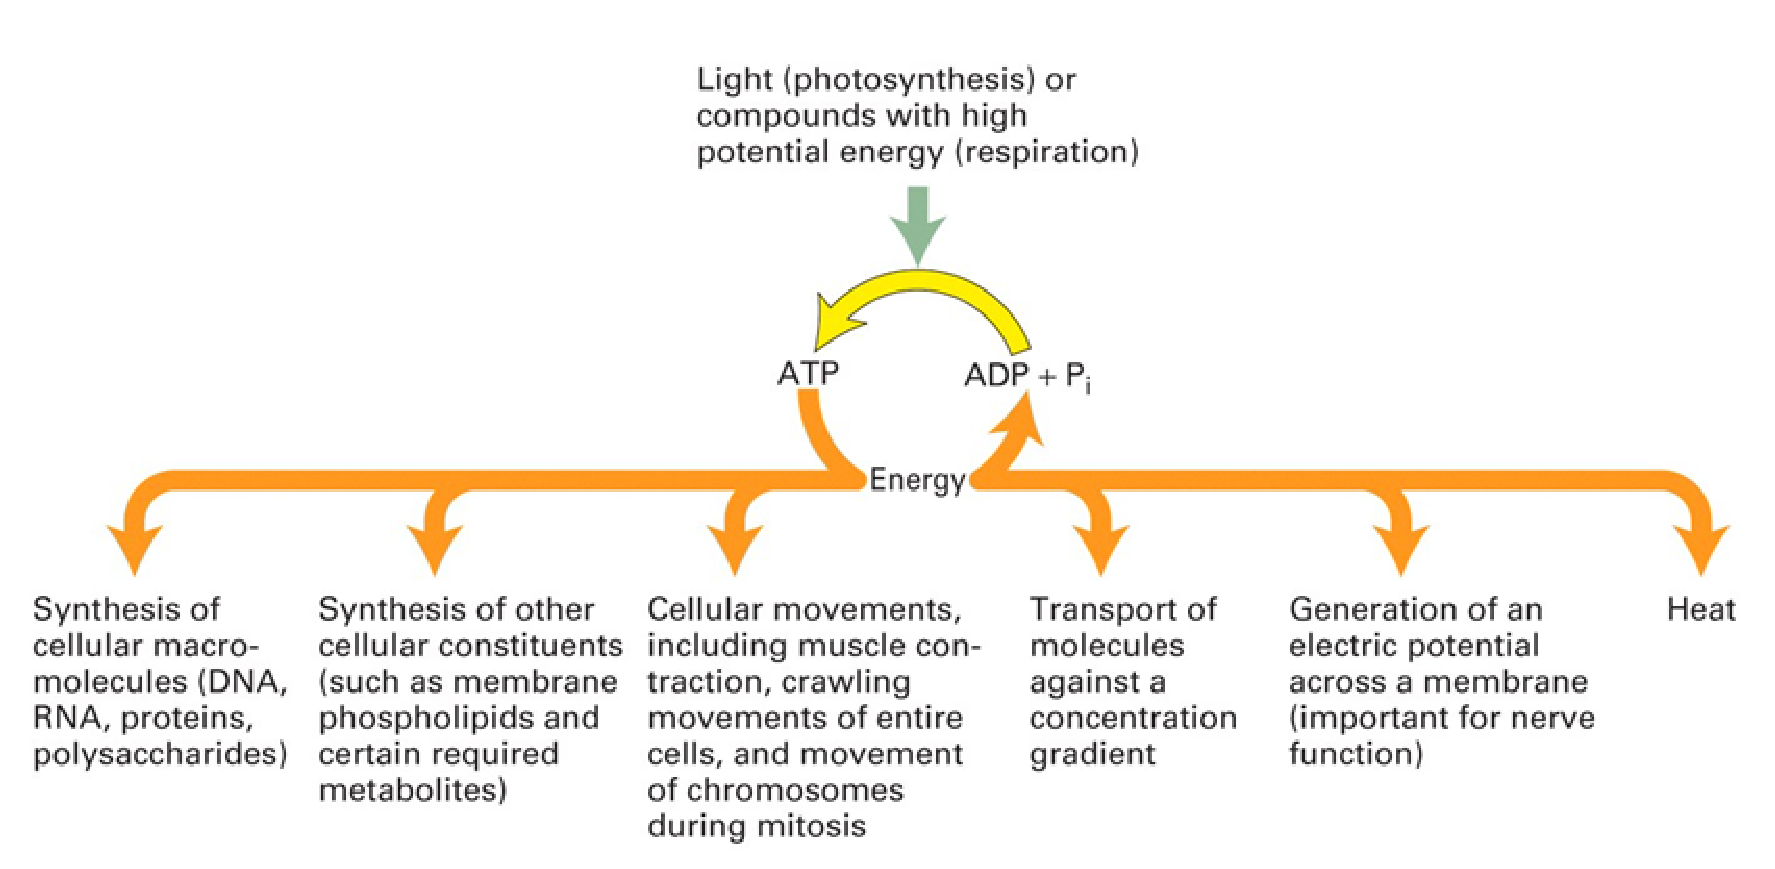
\includegraphics[height=5cm,
    angle=0]{./images/ATP_lifecycle.eps}}
  \caption{ATP lifecycle}
  \label{fig:ATP_cycle}
\end{figure}

\begin{figure}[hbt]
  \centerline{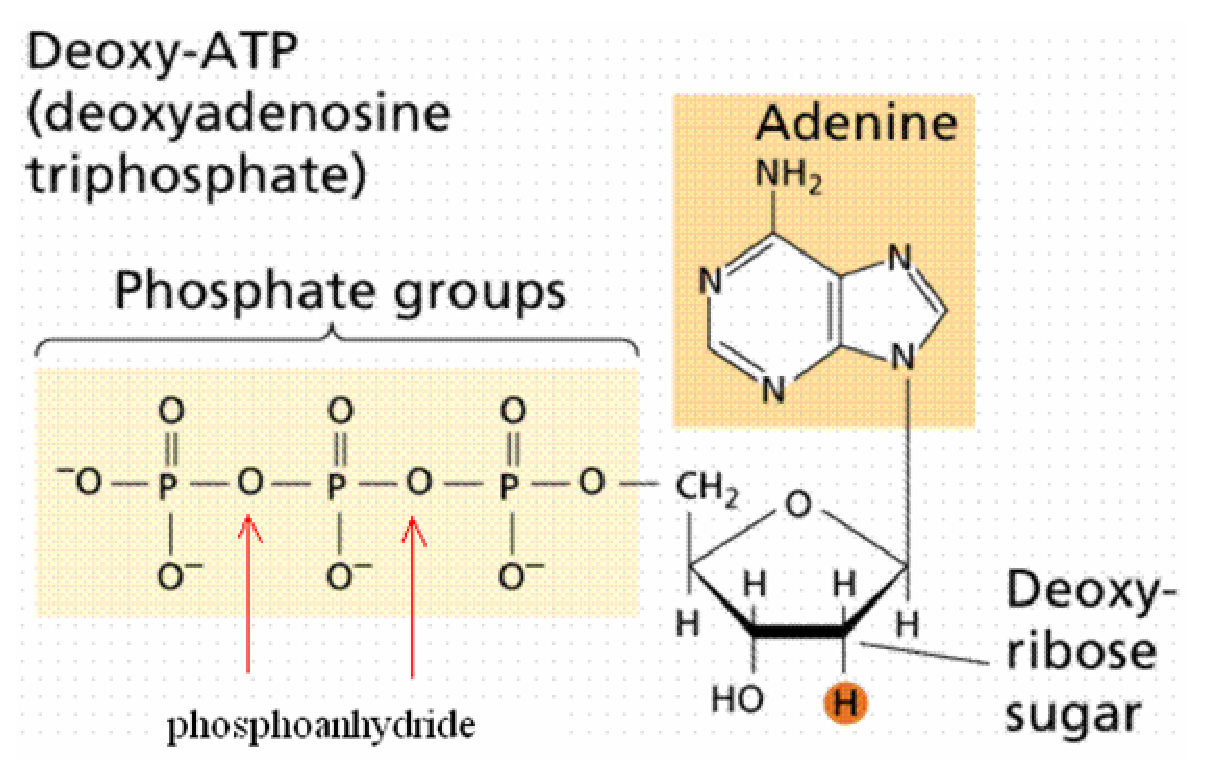
\includegraphics[height=5cm,
    angle=0]{./images/ATP_molecule.eps}}
  \caption{ATP molecule\footnote{\url{http://web.virginia.edu/Heidi/chapter1/Flash/figure1_3_atp.html
      }}}
  \label{fig:ATP_molecule}
\end{figure}

\textcolor{red}{How can ATP being an energy provider?}  -  ATP has two
phosphoanhydride bonds which link the three {\it phosphate groups}.
When each of these three groups are cleaved (in the
{\it hydrolysis process}), it releases a large amount of energy
$\Delta G^0=7.3$kcal/mol (rich-energy bonds).

\begin{figure}[hbt]
  \centerline{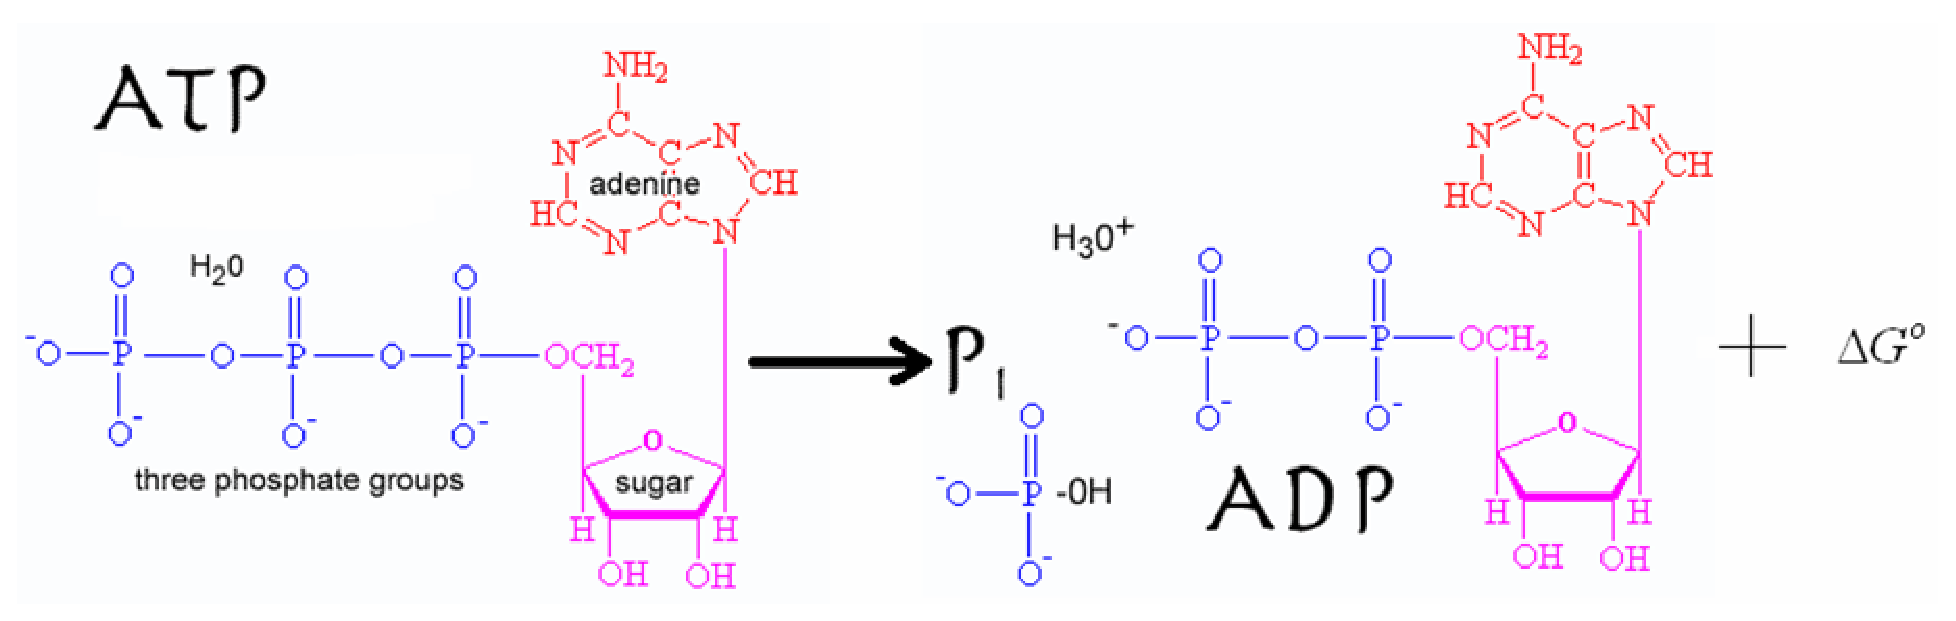
\includegraphics[height=4cm,
    angle=0]{./images/ATP_hydrolysis.eps}}
  \caption{ATP hydrolysis}
\label{fig:ATP_hydrolysis}
\end{figure}




\begin{figure}[hbt]
  \centerline{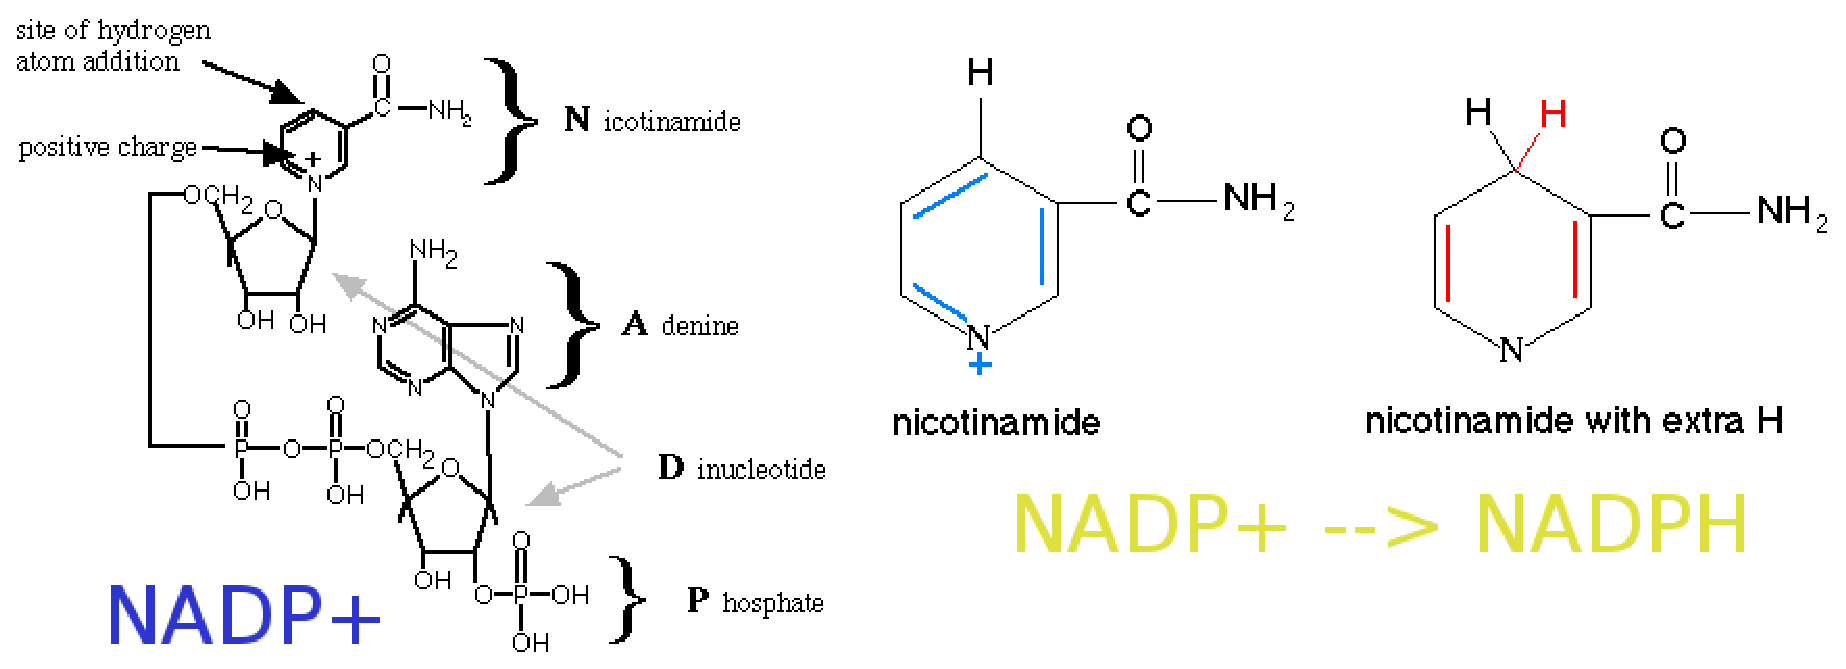
\includegraphics[height=4cm,
    angle=0]{./images/NADP_NADPH.eps}}
\caption{Conversion from NADP+ to NADPH}
\label{fig:NADP_NADPH}
\end{figure}


\begin{framed}
  The living state is characterized by the flow of energy through the organism.
\end{framed}

\subsection{ATP concentration}
\label{sec:ATP-concentration}

ATP content assays. ATP levels were measured using a method described previously
(Milakovic and Johnson, 2005). ATP content was measured using a FLUOstar Galaxy
microplate reader (BMG Labtech, Offenburg, Germany).

\subsection{How ATP generates energy: ATP-PC + Glycolytic system + oxidative
system}
\label{sec:enery-production-pathways}

Any muscle contraction/force exertion is due to a molecule called adenosine
triphosphate (ATP) - Sect.\ref{sec:ATP-overview}). Also in the brain, the
neurons also need ATP (Chap.\ref{chap:brain-energetic-demand}).

When an ATP molecule is combined with water the last of three phosphate groups
splits apart and produces energy. This breakdown of ATP for muscle contraction
results in adenosine diphosphate (ADP). By default, the floating ATP in the cell
is enough to provide up to 3 seconds of energy use.

\begin{mdframed}

Oxidative system - Sect.\ref{sec:oxidative-system} - is used primarily during
complete rest and low-intensity activity. Here, fats and carbs are the primary
substrates that are used. It can produce ATP through either fat (e.g. fatty
acids) or carbohydrate (Sect.\ref{sec:carbohydrates}).
Oxidative system is estimated to create approximately 10 calories per minute.

Carbohydrate is used first to produce ATP. However, in very long duration
activities (i.e., marathons), carbohydrates can be depleted and the body looks
to fat as the energy producer. Because fatty acids take more time to breakdown
than glucose, more oxygen is needed for complete combustion.

In extended activities protein can be used as a "last resort" for energy
production (in rare cases where carbohydrates are depleted and stored fat is
minimal). In such cases, it can supply as much as 18\% of total energy
requirements. The building blocks of protein - amino acids - can be either
converted into glucose (via gluconeogenisis - Sect.\ref{sec:gluconeogenesis}) or
other sources used in the Krebs cycle, such as acA. But understand protein
cannot supply energy at the same rate as carbohydrates and fats, thus it's
basically a non-issue).
\end{mdframed}

The limited stores of ATP must be replenished for work to continue; so chemical
reactions add a phosphate group back to ADP to make ATP
(Sect.\ref{sec:ATP-synthesis}).

\begin{enumerate}
  \item phosphagen system -   Sect.\ref{sec:phosphagen-system}):
  high power, short duration

So, maximum power declines around 12 seconds (during ATP-PC).

  \item glycolytic system - Sect.\ref{sec:glycolytic-system}: moderate
  power/short duration

Further intense activity up to approximately 30 seconds (during the time
glycolytic system kick in) results in lactic acid accumulation, a decrease in
power, and consequent muscle fatigue. If you are running, swimming, biking, or
walking long distances you will be using this energy system.

  \item oxidative - Sect.\ref{sec:oxidative-system}: low power/long duration

Exerting further effort up to approximately 50 seconds results in another drop
in power due to the shift in dependence on the oxidative system.
This is the primary source of ATP at rest and during low intensity exercise.
After about 90 seconds of continuous physical exertion this energy system will
kick in; but if you continue to exercise longer, other ATP-production systems
need also to kick in.

\end{enumerate}


\subsection{ADP}
\label{sec:ADP}

\subsection{GTP}
\label{sec:GTP}

Guanosine-5'-triphosphate (GTP) also has the role of a source of energy or an
activator of substrates in metabolic reactions, like that of ATP
(Sect.\ref{sec:GTP}), but more specific.

\subsection{Dibasic phosphate (HPO4$^{2-}$)}
\label{sec:dibasic-phosphate}

Dibasic  phosphate  (\ce{HPO_4^{2-}})



\subsection{Pi: inorganic phosphate (orthophosphate)}
\label{sec:inorganic-phosphate}
\label{sec:orthophosphate}
\label{sec:P_i}

Inorganic phosphate (Pi) is an essential nutrient to living organisms. It plays
a key role in diverse biological processes.
It is required as a component of the energy metabolism, kinase/phosphatase
signaling and in the formation and function of lipids, carbohydrates and nucleic
acids and, at systemic level, it plays a key role for normal skeletal and dentin
mineralization.

Maintenance of proper Pi homeostasis is a critical event.
serum Pi level is maintained within a narrow range through an elaborate network
of humoral interactions and feedback loops involving intestine, kidney,
parathyroid gland and bone, and depends on the activity of a number of hormones,
including parathyroid hormone, 1,25-dihydroxy vitamin D, and fibroblast growth
factor 23 as major regulators of Pi homeostasis. The kidney is a major regulator
of Pi homeostasis and can increase or decrease its Pi reabsorptive capacity to
accommodate Pi need.

\begin{enumerate}
  \item  Type II sodium-dependent phosphate (Na/Pi) cotransporter (NPT2) is the
  major molecule in the renal proximal tubule and is regulated by Pi,
  parathyroid hormone and by 1,25-dihydroxyvitamin D
  %https://www.ncbi.nlm.nih.gov/pubmed/15256067

  \item
\end{enumerate}

Relevantly, Pi is emerging as an important signalling molecule capable of
modulating multiple cellular functions by altering signal transduction pathways,
gene expression and protein abundance in many cell types.
\begin{itemize}
  \item to cancer - %https://www.ncbi.nlm.nih.gov/pmc/articles/PMC4675902/
\end{itemize}

However, little is known about the initial events involving the detection of
changes in serum or local Pi concentrations and the subsequent downstream
regulation cascade

%https://www.ncbi.nlm.nih.gov/pubmed/23394088




\subsection{Citric Acid (citrate)}
\label{sec:citric-acid}
\label{sec:citrate}
\label{sec:citrate-synthase}

\begin{mdframed}
Citric acid exists in greater than trace amounts in a variety of fruits and
vegetables, most notably citrus fruits, e.g. lemons and limes with as much as
8\% of dry weight (or 47 g/L in the juices). NOTE: Citrate can also be used as
calcium buffer (Sect.\ref{sec:citrate-maleate}).
\end{mdframed}


Citric acid (\ce{C6H8O7}), or more precisely {\bf Citrate ion}, is
a type of tricarboxylic acid (i.e. containing three -COOH carboxyl groups)
A {\bf citrate} is a derivative of citric acid, i.e. the salts, esters, and
the polyatomic anion found in solution.
\begin{itemize}
  \item salt form: trisodium citrate \ce{C6H5O7^{3-}} or \ce{C3H5O(COO)3^{3-}}
  \item ester form: triethyl citrate.
\end{itemize}

Citrate is the result of the transfer of a two-carbon acetyl group from
acetyl-CoA to the four-carbon acceptor compound (oxaloacetate) to form a
six-carbon compound (citrate). \textcolor{blue}{This is the first reaction in
citric acid cycle} (Sect.\ref{sec:krebs-cycle}).

{\bf Citrate synthase} catalyzes citrate using oxaloacetate
(Sect.\ref{sec:oxaloacetate}) and acetyl-CoA
\begin{equation}
\text{acetyl-CoA  + oxaloacetate } + \ce{H2O -> } \text{ citrate + CoA-SH};
\Delta G^\circ = -32.2 \text{ kJ/mol}
\end{equation}
NOTE: It is also used as mitochondria's marker -
Sect.\ref{sec:mitochondria-marker}.

The enzyme citrate synthase is \textcolor{red}{inhibited} by high ratios of
ATP:ADP, acetyl-CoA:CoA, and NADH:NAD, as high concentrations of ATP,
acetyl-CoA, and NADH show that the energy supply is high for the cell. It is
also inhibited by succinyl-CoA, which resembles Acetyl-coA and acts as a
uncompetitive inhibitor.
Citrate inhibits the reaction and is an example of product inhibition.

Citrate can be removed from the citric acid cycle and carried across the inner
mitochondrial membrane into the cytosol via the tricarboxylate anion carrier
system. In the cytosol, citrate is cleaved by ATP citrate lyase into acetyl-CoA
(Sect.\ref{sec:Acetyl-CoA}) and oxaloacetate (Sect.\ref{sec:oxaloacetate}).
Oxaloacetate is returned to mitochondrion as malate (and then converted back
into oxaloacetate to transfer more acetyl-CoA out of the mitochondrion)
Because of this, oxaloacetate is replenished in mitochondria after each cycle.
\url{https://www.sciencedirect.com/topics/neuroscience/acetyl-coa}


\subsection{Oxaloacetate}
\label{sec:oxaloacetate}

Oxaloacetate (4-carbon): $\ce{HO2CC(O)CH2CO2H}$
\begin{verbatim}
pyruvate + ATP + CO2 --[pyruvate carboxylase]--->   oxaloacetate + ADP + Pi
\end{verbatim}

Inside matrix, pyruvate, besides converting to acetyl-CoA, can also be converted
into oxaloacetate. Oxaloacetate play 2 roles:
\begin{enumerate}
  \item  which helps to create citrate
(Sect.\ref{sec:citrate}), i.e. accelerating energy production in TCA cycle -
Sect.\ref{sec:krebs-cycle} during urgent energy demand.


Oxaloacetate is also a potent inhibitor of Complex II -
Sect.\ref{sec:complex-II-mito}.

  \item involves into amino acid synthesis,   and fatty acid synthesis.

  \item (once it gets to cytosol) oxaloacetate is also involved in
  gluconeogenesis (Sect.\ref{sec:gluconeogenesis}), urea cycle, glyoxylate
  cycle.

\begin{verbatim}
oxaloacetate   get to cytosol by passing through
          MIM via malate-oxaloacetate shuttle
          MOM via non-selective permeable porin
\end{verbatim}

\end{enumerate}

\subsection{Creatine phosphokinase}
\label{sec:creatine-phosphokinase}

In 1962, with the ability to block creatine phosphokinase, ATP
was then proved to be coupled to mechanical energy release


\subsection{Concentrations}
\label{sec:concentrations-ATP}
\label{sec:concentrations-ADP}
\label{sec:concentrations-Creatine}
\label{sec:concentrations-H2O}

The level of ATP in the cell is stabilized by the enzyme creatine phosphokinase
(Sect.\ref{sec:creatine-phosphokinase}).


In resting muscle: [ATP]= 4 mM, [ADP]=0.013 mM, [creatine phosphate] = 25 M,
[creatine] = 13 mM. ATP levels do not change more than 10\% in vivo between rest
and vigorous exercise; with the helps of ATP-stabilization protein.

Water concentration: \ce{[H2O]} = 55.5 M.

Given $K_w = [H^+][OH^-]$, at 25$^o$C, $K_w = 1.0 \times 10^{-14}$. In
the following reaction
\begin{equation}
  \label{eq:5}
  \ce{H20 <=> H+ + OH-}
\end{equation}
we have $K_{eq} = \frac{[H^+][OH^-]}{[\ce{H2O}]} = \frac{K_w}{[\ce{H2O}]}$.

From catabolic reaction (Sect.\ref{sec:catabolic-reaction}), one gram of
carbohydrate was oxidized to \ce{CO2} and \ce{H2O}, 4.1 kcal was released. The
values for 1.0g fat or 1.0g protein was 9.1kcal and 4.1kcal, respectively.

\section{Flavoprotein}
\label{sec:flavoprotein}

Flavoproteins are proteins that contain a nucleic acid derivative of riboflavin:
the flavin adenine dinucleotide (FAD - Sect.\ref{sec:FAD}) or flavin
mononucleotide (FMN) - Sect.\ref{sec:FMN}.

One flavoprotin was first found in 1879, when they isolated as a bright-yellow
pigment from cow's milk. It was intially term {\it lactochrome}, and later was
known as {\bf riboflavin}.
By the early 1930s, this same pigment had been isolated from a range of sources, and
recognised as a component of the vitamin B complex

\begin{enumerate}
  \item  5-10\% of flavoproteins have a covalently linked FAD
  
  FAD-binding sites can be divided into more than 200 different types
  
  \item Flavoproteins are mainly located in the mitochondria.
  
  Of all flavoproteins, 90\% perform redox reactions and the other 10\% are
  transferases, lyases, isomerases, ligases.
  
  
  \item in human: 90 flavoproteins are encoded in the human genome; about 84\%
  require FAD, and around 16\% require FMN, whereas 5 proteins require both
\end{enumerate}

There are many flavoproteins besides components of the succinate dehydrogenase
complex, including $\alpha$-ketoglutarate dehydrogenase and a component of the
pyruvate dehydrogenase complex;



\section{Fatty acid metabolism}
\label{sec:catabolic-energy-metabolism}
\label{sec:catabolic-reaction}
\label{sec:fatty-acid-metabolism}

Fatty acid metabolism consists of catabolic processes that generate energy, and
anabolic processes that create biologically important molecules (triglycerides,
phospholipids, second messengers, local hormones and ketone bodies).

Fatty acids are stored as triglycerides - Sect.\ref{sec:triglycerides}


\subsection{Energy storage}
\label{sec:energy-storage}


Energy substrates are the chemicals that are required to resynthesis ATP.
\begin{enumerate}
  \item PC - Sect.\ref{sec:phosphocreatine}

  \item glycogen - Sect.\ref{sec:glycogen}

  \item triglycerides (stored fat) - Sect.\ref{sec:triglycerides}

\end{enumerate}

\subsection{triglycerides}
\label{sec:triglycerides}

Triglycerides are the main constituents of body fat in humans and other animals
(Sect.\ref{sec:fats}).


\subsection{---- Coenzyme-A (CoA, CoA-SH) and acetyl CoA}
\label{sec:CoA}
\label{sec:Acetyl-CoA}
\label{sec:coenzyme-A}

Coenzyme-A (CoA, CoA-SH) was discovered in 1947 by Fritz Albert Lipmann
as a catalytically active, heat-stable factor in pigeon liver extracts.
CoA is now known to be bound to acetic acid - and involve in citric acid cycle
which is the process discovered by Krebs in 1937 (Sect.\ref{sec:krebs-cycle}).
Both Krebs and Lipmann shared Nobel prize in 1953 for their work.

The formation of acetyl coenzyme A (or acetyl CoA) occurs inside the
mitochondria (in the case of eukaryotes) and in cytosol (in the case of
prokaryotes). However, in eukaryotes, we still have cytosolic acetyl-CoA and
cytosolic acetyl-CoA is used for fatty acid synthesis and the production of
cholesterol. As \textcolor{red}{acetyl-CoA cannot be transported out of the
mitochondrion}.
Thus, to have cytosolic acetyl-CoA, citrate (Sect.\ref{sec:citric-acid}) is
removed from the citric acid cycle and carried across the inner mitochondrial
membrane into the cytosol.

In mitochondria, acetyl-CoA is the product (break-down) of
\begin{enumerate}

  \item pyruvate (Sect.\ref{sec:pyruvate}) with coenzyme A (CoA-SH) under the
  so-called pyruvate dehydrogenase reaction
  (Sect.\ref{sec:pyruvate-to-acetyl-CoA}):

DETAILS:
\begin{equation}
\begin{split}
&\text{ if acetyl-CoA transfered to cytosol: acetyl-CoA ---> fatty acids} \\
&\text{ if acetyl-CoA remains inside matrix: acetyl-CoA involves TCA cycle}
\end{split}
\end{equation}

The chemical formula of acetyl CoA is two-carbon structure:
$\ce{CH3C(=O)SCoA}$. Due to the high energy of the thioester bond in
Acetyl-CoA, this link is unstable; i.e. the acetyl group can be easily
transferred to another molecules, which explains the reason why Acetyl-CoA is
used as a universal intermediate for transmitting the \ce{C_2} fragment
(Sect.\ref{sec:citric-acid-cycle}).

% \begin{equation}
%   \label{eq:9}
%   \text{pyruvate} + \ce{O2 + NAD+ + CoA -> \text{Acetyl-CoA} + CO2 + NADH}
% \end{equation}
% \textcolor{red}{From this equation, we now understand the true role of
%   \ce{O2} in the cell}.

  \item lipids of saturated fatty acids (by $\beta$-oxidation -
  Sect.\ref{sec:beta-oxidation})

  \item ketone bodies - Sect.\ref{sec:ketone-bodies}
\end{enumerate}
%CoA-SH - Sect.\ref{sec:CoA}


\begin{mdframed}
Coenzyme-A (CoA, coenzyme Acetyl, CoA-SH or HSCoA) is a co-enzyme and plays an
important role
\begin{itemize}
  \item   All genomes sequenced to date encode enzymes that use coenzyme A as a
  substrate
  \item around 4\% of cellular enzyme uses CoA as a substrate
\end{itemize}

In human, CoA biosynthesis requires cysteine, pantothenate, and adenosine
triphosphate (ATP). CoA is composed of two main parts,
Fig.~\ref{fig:CoA}.
\begin{itemize}
  \item a long protein-like chain
  \item -SH group

The -SH group is very important as it is highly reactive, and can link to
carboxylic acid molecules (e.g. pyruvate - Sect.\ref{sec:pyruvate}) via {\it
thioester bond}, forming Acetyl CoA.

\end{itemize}

\end{mdframed}

\begin{figure}[hbt]
  \centerline{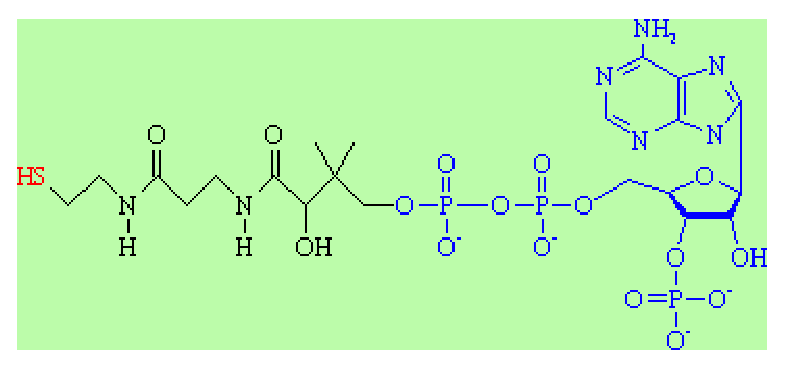
\includegraphics[height=3cm,
    angle=0]{./images/CoA.eps}}
  \caption{CoA with 2 main parts: long protein-like chain (shown in
    black) joined with ADP (shown in blue); the second and important
    part is the sulph-hydryl (-SH) group (shown in red) }
  \label{fig:CoA}
\end{figure}



\subsection{---- Pyruvate (pyruvic acid)}
\label{sec:pyruvate}
\label{sec:pyruvic-acid}

{\bf Pyruvate} ($\ce{CH3C(=O)C(=O)O-}$ or pyruvate$^{-}$) is the ester form of
the 3-carbon {\bf pyruvic acid}. Pyruvate is the product of the glycolysis in the cytosol -
Sect.\ref{sec:glycolysis}, in that one glucose (or one glucose-6P) molecules
produce 2 pyruvate molecules, along with other molecules.
\begin{itemize}
  \item  In the heart: the pyruvate is typically derived from both glycolysis
  and lactate oxidation in almost equal amounts, because the heart expresses
  high levels of the LDH-B isoenzyme which favours the conversion of lactate to
  pyruvate (Sect.\ref{sec:lactate-oxidation}).

  \item  Normal pyruvate concentration in a cell is about 0.1 mM.
%  \item
\end{itemize}

\begin{figure}[hbt]
  \centerline{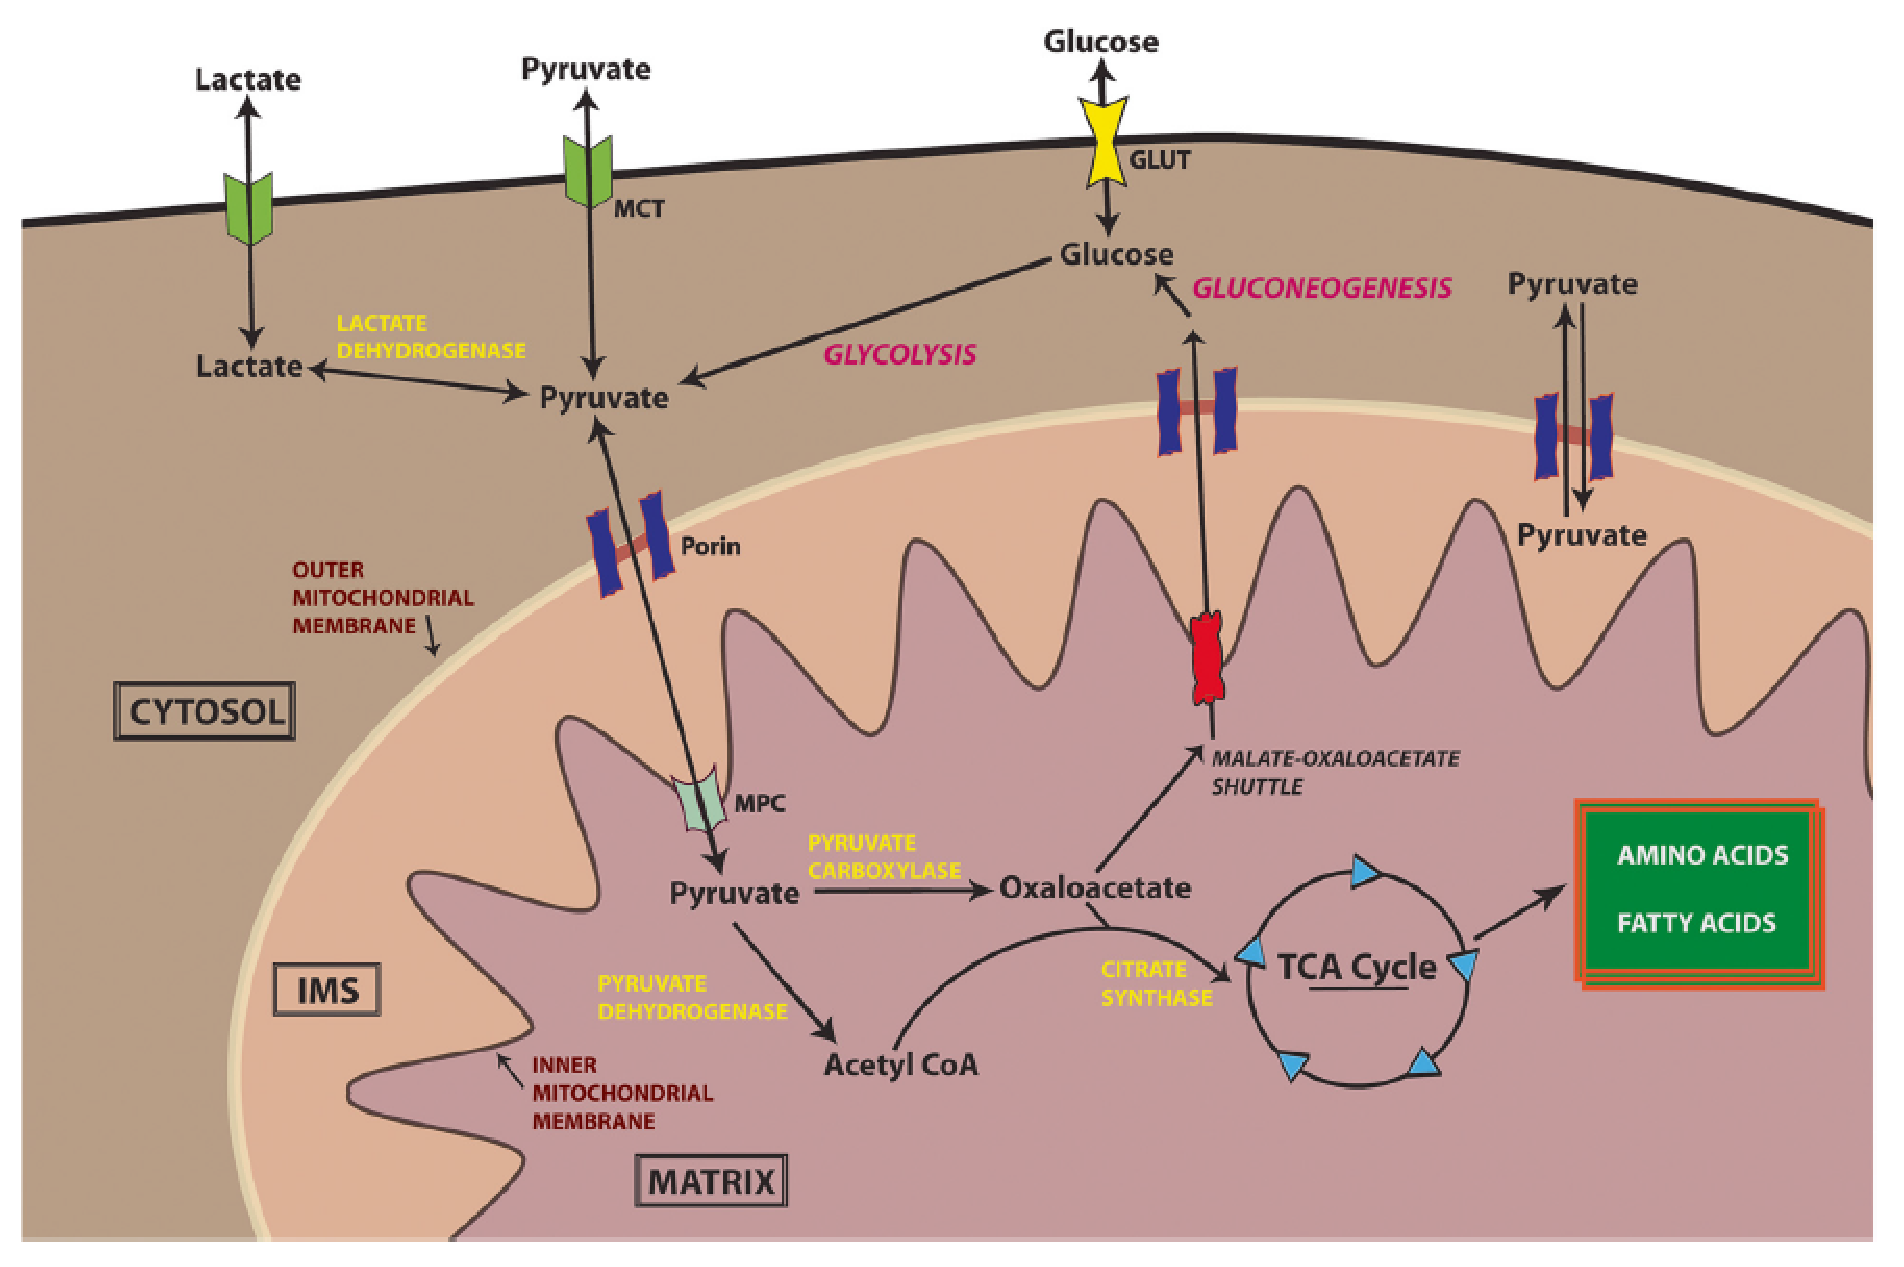
\includegraphics[height=6cm,
    angle=0]{./images/pyruvate-pathways.eps}}
\caption{An overview of pyruvate pathways}
\label{fig:pyruvate-pathways}
\end{figure}


Pyruvate may follow different pathways, Fig.\ref{fig:pyruvate-pathways}.
\begin{itemize}

  \item (physiological condition) most pyruvates will get into the mitochondria
  - Sect.\ref{sec:pyruvate-transporter}

Once within the mitochondrial matrix, pyruvate may be diverted into two
disparate paths.
\begin{enumerate}
  \item  pyruvate is carboxylated to form oxaloacetate, which can be used for
  gluconeogenesis.
  \item  pyruvate is decarboxylated to form Acetyl-CoA
\end{enumerate}

Once within the mitochondrial matrix, pyruvate may be diverted into two
disparate paths
\begin{enumerate}
  \item \textcolor{red}{converted into acetyl-CoA} is discussed in
  Sect.\ref{sec:pyruvate-to-acetyl-CoA}.

\begin{verbatim}
// pyruvate is first transported into mitochondria's matrix
//  before it involves
pyruvate --[rich-oxygen condition]--> Acetyl CoA
\end{verbatim}
% The two-carbon structure (as in pyruvate which is a
% metabolite of glucose) is combined with coenzyme A to for acetyl-CoA


  \item \textcolor{red}{converted into oxaloacetate} -
  Sect.\ref{sec:oxaloacetate}
\end{enumerate}



  \item  However, remember that not all pyruvate created during glycolysis goes
  into the mitochondria. Many of cytosolic pyruvate got converted to
  L-lactate (Sect.\ref{sec:Lactate-production}) in a oxygen-depleted enviroment
  in the cytosol called {\it anaerobic
  glycolysis} (Sect.\ref{sec:anaerobic-glycolysis}).

Once created in the cytoplasm, under normal conditions approximately 5\% of the
pyruvate is converted to lactate by lactate dehydrogenase in the cytoplasm.
\begin{verbatim}
pyruvate --[low-oxygen condition]--> lactate
       (not common in physiological state)
\end{verbatim}

\end{itemize}


As NADH is the high-energy molecule, and pyruvate takes some time to get to
mitochondria (or cannot be utilized by the mitochondria (due to limited oxygen
supply - NOTE: ETC requires oxygen - Sect.\ref{sec:electron-transport-chain})),
NADH is reoxidized by reducing pyruvate to lactic acid by

{\tiny
\begin{verbatim}
Pyruvate + NADH + H+  ----[lactate dehydrogenase]---> lactic acid  + NAD+ + energy

Lactic acid -----------> L-lactate
\end{verbatim}
}

NOTE: $\Delta G = -25.1$ kJ/mol.


\begin{mdframed}
Anaerobic glycolysis is thought to have been the primary means of energy
production in earlier organisms before oxygen was at high concentration in the
atmosphere and thus would represent a more ancient form of energy production in
cells.
\end{mdframed}


% \begin{verbatim}
% pyruvate --[anaerobic]--> lactate
%
% pyruvate --[aerobic]--> Acetyl CoA
% \end{verbatim}


SUMMARY: Depending the locations (in mitochondria or in cytosol), pyruvate can
be converted to different things
\begin{enumerate}

  \item back to glucose (in cytosol) via gluconeogenesis -
  Sect.\ref{sec:gluconeogenesis}

  \item Oxaloacetic acid (oxaloacetate) - Sect.\ref{sec:oxaloacetate}

  \item to fatty acids

  \item to acetyl-CoA (inside mitochondria's matrix)

Pyruvate molecules produced by glycolysis are actively transported across the
inner mitochondrial membrane, and into the matrix. Here, they are oxidized to
form Acetyl-CoA - Sect.\ref{sec:stage-3}. In particular, pyruvate is converted
into acetyl-coenzyme A (Acetyl-CoA) - that can enter the Krebs cycle
(Sect.\ref{sec:krebs-cycle}). Sect.\ref{sec:Acetyl-CoA} explains this convertion
process.

  \item lactic acid - Sect.\ref{sec:glycolysis-anaerobic}

\end{enumerate}



\begin{figure}[hbt]
  \centerline{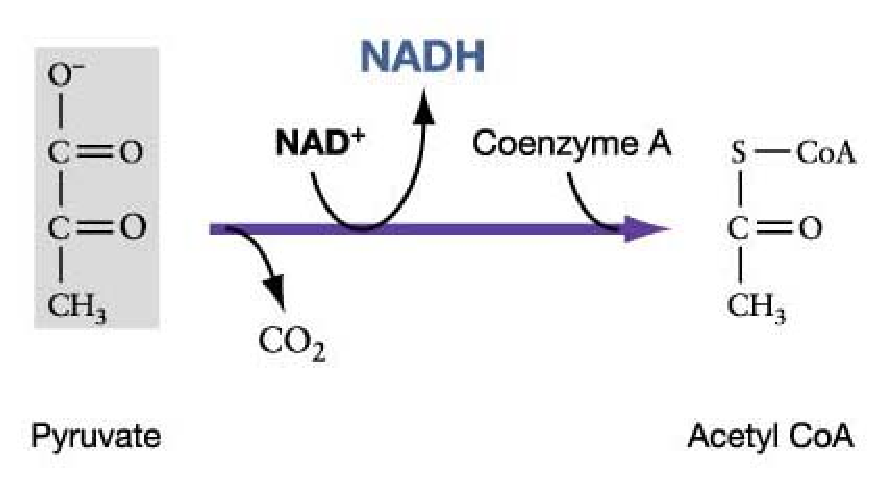
\includegraphics[height=5cm,
    angle=0]{./images/pyruvate2AcetyleCoA.eps}}
\caption{Producing Acetyl CoA from pyruvate}
\label{fig:pyruvate2AcetylCoA}
\end{figure}

\subsection{pyruvate transporters (MPC = mitochondrial pyruvate carriers): MPC1,
MPC2}
\label{sec:pyruvate-transporter}
\label{sec:pyruvate-translocase}

First, pyruvate (the product of glycolysis) is transported into the matrix of
mitochondria. Three layers must be traversed: the outer mitochondrial membrane,
the intermembrane space, and the inner mitochondrial membrane.
\begin{itemize}
  \item  Transport of pyruvate across the mitochondrial outer membrane
  (MOM) appears to be easily accomplished via large non-selective channels such
  as voltage-dependent anion channels/porin, which enable passive diffusion (Benz,
  1994).

% Permeation of hydrophilic solutes through mitochondrial outer membranes: review on mitochondrial porins.
% Benz R
% Biochim Biophys Acta. 1994 Jun 29; 1197(2):167-96.
Indeed, deficiencies in these channels have been suggested to block pyruvate
metabolism.

% \begin{enumerate}
%
%   \item passing MOM into inter-membrane regions: appears to be
%   easily accomplished via large non-selective channels such as voltage-dependent anion channels/porin, which
%   enable passive diffusion
%
%   \item from inter-membrane regions, it passes MIM via MPC is far more
%   restrictive - Sect.\ref{sec:pyruvate-transporter}, and \textcolor{red}{that
%   pyruvate transpot can be a rate-limiting factor for pyruvate oxidation - the
%   next stages of ATP production}.
%
% \end{enumerate}

  \item  The movement through the mitochondrial inner membrane (MIM) is far more
  restrictive,  and it needs mitochondrial pyruvate transporter
  (Sect.\ref{sec:pyruvate-transporter}).

\textcolor{red}{Pyruvate transport across MIM can be a rate-limiting factor for
pyruvate oxidation - the next stages of ATP production}.
%  \item
\end{itemize}

\begin{mdframed}
Initially it was proposed that pyruvate was able to cross the MIM in
its undissociated (acid) form but evaluation of its biochemical properties show that
pyruvate is largely in its ionic form within the cell and should therefore
require a transporter.
\begin{itemize}
  \item  Using protein-free liposomes it was found that pyruvate did indeed have
  the ability to cross membranes directly.

  A potential caveat of these studies was the use of 100 mM pyruvate, a
  concentration that is roughly 1,000-fold higher than would is typically
  encountered within the cell

  \item   In addition, artificial membranes used in these studies may not replicate the
  permeability and other properties of the mitochondrial inner membrane.

\end{itemize}
Later studies unequivocally demonstrated transporter-mediated pyruvate movement
(Papa et al., 1971).
Although much remains unknown, two independent studies have rigorously tested
two mitochondrial inner membrane proteins: MPC1 and MPC2 {\bf Review: Schell,
Rutter (2013), McCommis, Finck (2015)}

{\it The identification of these transporter constituents opens the door to the
identification of novel compounds that modulate MPC activity, with potential
utility for treating diabetes, cardiovascular disease, cancer, neurodegenerative
diseases, and other common causes of morbidity and mortality.}

\end{mdframed}

Our current understanding is that two proteins, {\bf mitochondrial pyruvate
carriers} MPC1 and MPC2, and they must form a hetero-oligomeric complex in the
IMM (necessary and sufficient) to facilitate pyruvate transport. Its old names
are BRP44L and BRP44, respectively.
\textcolor{red}{rate-limiting}:
\begin{itemize}
  \item  pyruvate uptake found the rate to be quite low $V_\max = 0.54 \pm 0.03$
  (nmol per minute per mg of mitochondrial protein) (Halestrap, 1975)

% The mitochondrial pyruvate carrier. Kinetics and specificity for substrates and inhibitors.
% Halestrap AP
% Biochem J. 1975 Apr; 148(1):85-96.


\end{itemize}

\textcolor{red}{MPC's inhibitors}:
\begin{enumerate}
  \item  Halestrap and colleagues identified and characterized an inhibitor of
  mitochondrial pyruvate transport. $\alpha$-Cyano-4-hydroxycinnamate (CHC)
   inhibit pyruvate oxidation and found to do this by blocking mitochondrial
  pyruvate transport

The inhibitor has no effect on ruptured mitochondria
In this way it is possible to ascribe the inhibitory effect to be at the
membrane rather than a mitochondrial enzyme.

CHC and other cinnamate-based inhibitors resemble the enol form of pyruvate with
an attached aromatic ring

Expanding upon the discovery of cinnamates as MPC inhibitors, it was shown that
these compounds also inhibit the transport of pyruvate across the plasma
membrane of erythrocytes, but they do so much less potently, suggesting that the
two membranes have different transporters

Respiration experiments in the presence of 60 mM pyruvate became insensitive to
CHC. Therefore, while CHC doesn't appear to be a competitive inhibitor, high
concentrations of pyruvate (60 mM) can overcome inhibition of transport.

  \item Pande and Parvin (1978) provided new data for the inhibition of the
  transporter by cinnamates.

Even after CHC-treated mitochondria were washed with 60 mM pyruvate,
concentrations of pyruvate that would normally drive pyruvate oxidation (1 mM)
failed to do so, suggesting the mechanism of inhibition is non-competitive.


\end{enumerate}




\subsection{pyruvate dehydrogenase complex (PDC)}
\label{sec:pyruvate-dehydrogenase-complex}
\label{sec:prosthetic-group}

The {\it pyruvate dehydrogenase complex} (PDC) converts pyruvate into acetyl-CoA
(Sect.\ref{sec:pyruvate-to-acetyl-CoA}). \textcolor{red}{The reaction by E1 is
considered to be the rate-limiting step for the pyruvate dehydrogenase complex
(PDHc).}


PDC is a large multi-enzyme complex composed of three enzymes involving five
cofactors.
\begin{enumerate}
  \item pyruvate dehydrogenase (E1):  uses thiamine pyrophosphate (TPP or
  vitamin B1) as its prosthetic group.

E1 is a tetrameric with two alpha- and two beta-subunits. Some bateriaal E1 has
two similar subunits. The $\alpha$- subunit binds magnesium ion and
pyrophosphate fragment while the $\beta$-subunit binds pyrimidine fragment of
TPP.

  \item dihydrolipoyl transacetylase (E2): uses lipoamide and coenzyme A (also
  known as coASH) as its prosthetic groups.

  \item dihydrolipoyl dehydrogenase (E3):  uses flavin adenine dinucleotide
  (FAD) and nicotinamide adenine dinucleotide (\ce{NAD^+}) as its cofactors.
\end{enumerate}

Note: Prosthetic groups are molecules that are covalently bonded to an enzyme.
\url{https://en.wikipedia.org/wiki/Pyruvate_dehydrogenase_complex}


Pyruvate dehydrogenase complex is activated by mitochondrial calcium
concentration ([$\Ca$]), and inhibited when the [ATP]:[ADP] ratio,
[\ce{NAD^+}]:[NADH] ratio, or [acetyl-CoA]/[CoA] ratio is increased.






\subsection{Lipolysis}
\label{sec:lipolysis}

Lipolysis is the breakdown of lipids (Sect.\ref{sec:lipids})

\section{Photosynthesis}

Photosynthesis is often described as the reverse of cellular respiration.
\begin{itemize}
  \item  Cellular respiration is the process of utilizing oxygen \ce{O2} and
  food molecules to create energy, carbon dioxie \ce{CO2}, water \ce{H2O}, and waste
products. Respiration breaks down complex molecules to release energy that is
used to make ATP.

   \item In the opposite direction, photosynthesis takes energy from photons and
   uses it to build complex molecules.
\end{itemize}
However both systems use an electron transport chain (ETC) and associated proton
pump and ATP synthase.

The electrons, after receiving light energy, carry energy and enter the ETC -
Sect.\ref{sec:ETC}). NOTE:  in respiration the electrons are provided by organic
food molecules such as NADH, \ce{FADH2} as the product of Kreb cycle
(Sect.\ref{sec:krebs-cycle}).

The ETC uses the energy (provided by the electrons) to pump protons $\H$ across
the MIM (Sect.\ref{sec:MIM-mito}), creating a strong gradient with higher
proton concentration in the inter-membrane region. The protons pass back
into the matrix through ATP synthase, a process also driving the production of
ATP (see more details in Sect.\ref{sec:ETC}).

\section{Insulin}
\label{sec:insulin}

As the level of glucose in the body is so important, glucose
metabolism is regulated by {\bf insulin}.

Insulin is synthesized in $\beta$-cells of the islets of
Langerhans. Insulin secretion from $\beta$-cells of the pancreas is
principally regulated by plasma glucose levels. Thus, the increase
uptake of glucose leads to the increase in insulin metabolism, which
in turns lead to an elevation of ATP/ADP ratio. More ATP will inhibit
ATP-sensitive \ce{K+} channel (KATP channel).

% \section{Summary}
% \label{sec:summary}

\section{Gluconeogenesis}
\label{sec:gluconeogenesis}

\textcolor{red}{{\bf Gluconeogenesis}}: Gluco - glucose; genesis - creation.
Gluconeogenesis reaction pathway is essentially the reverse of glycolysis with a
couple of changes. Gluconeogenesis is a pathway consisting of a series of 11
enzyme-catalyzed reactions to create glucose (Sect.\ref{sec:glucose}) from
glycogen (Sect.\ref{sec:glycogen}). This mainly happens in either the liver or
kidney, in the mitochondria or cytoplasm of those cells.

The regulatory molecule in this case is glucagon which achieves the opposite of
insulin (this initiates the conversion of glucose into glycogen).


\subsection{in mitochondrion}

Gluconeogenesis begins in the mitochondria with the formation of oxaloacetate by
the carboxylation of pyruvate (Sect.\ref{sec:oxaloacetate}), and requires 1 ATP.

\begin{verbatim}
pyruvate + ATP --[pyruvate carboxylase]--------->   oxaloacetate
               [stimulated by [acetyl-CoA] high level]
               [inhibited by ADP and glucose high levels]


oxaloacetate  + NADH  ----------> malate
   (transfer malate to cytosol)

(in cytosol)
malate + NAD+   ------------>   oxaloacetate

oxaloacetate   ------------->  phosphoenol pyruvic acid

[next is reverse steps in glycolysis]
\end{verbatim}

\section{Glycerol}
\label{sec:glycerol}
\label{sec:glycerol-phosphorylation}

The phosphorylation of glycerol is a necessary step in forming the phospholipids
called glycerophospholipid (Sect.\ref{sec:glycerophospholipid}) that comprise cell
membranes. The product of glycerol phosporylation, glycerol-3-phosphate  is used
in the synthesis of phospholipids.

This step actually consists of two reactions: (1) the phosphorylation of
glycerol (by glycerol kinase found in liver), and (2) the dephosphorylation of
ATP (the free-energy-currency molecule).

{\tiny
\begin{equation}
\begin{split}
&\text{// non-spontaneous reaction: phosphorylation of glycerol} \\
&\text{glycerol +  \ce{HPO_4^{2-}}  ---[..]-->
 (Glycerol-3-phosphate)$^{2-}$ + \ce{H2O}} ;  \Delta G^\circ = +9.2 \text{kJ/mol} \\
&\text{// spontaneous reaction:} \\
&\ce{ATP^{4-}  + H2O} \text{ --[]-->} \ce{ADP^{3-} + HPO_4^{3-} + H+}  ;
 \Delta G^o = -30.5 \text{ kJ/mol} \\
&---------------------------------- \\
&\text{   Glycerol + \ce{ATP^{4-}} -[glycerol kinase]-> } \\
&\text{        (Glycerol-3-Phosphate)$^{2-}$ + ADP$^{3-}$ + H$^{+}$  ;
$\Delta G^\circ$ = -21.3 kJ/mol}
\end{split}
\end{equation}
}

Glycerol kinase is a large protein comprised of about 500 amino acids.X-ray
crystallography of the protein shows us that there is a deep groove or cleft in
the protein where glycerol and ATP both attach. Because the enzyme holds the ATP
and the glycerol in place, the phosphate can be transferred directly from the
ATP to glycerol.
Thus, instead of two separate reactions where ATP loses a phosphate (Equation 2)
and glycerol picks up a phosphate (Equation 1), the enzyme allows the phosphate
to move directly from ATP to glycerol.

\section{Triacylglycerol (TAG)}
\label{sec:triacylglycerol}

In hepatocytes (liver cells), free fatty acids are esterified with
glycerol-3-phosphate to generate triacylglycerol (TAG). TAG is stored in lipid
droplets in hepatocytes or secreted into the circulation as very low-density
lipoprotein (VLDL) particles.


\section{Peroxisome}
\label{sec:peroxisome}


Peroxisom is a type of organelle  known as a microbody, found in virtually all
eukaryotic cells Peroxisome  involved in catabolism of fatty acids, etc.
They also contain approximately 10\% of the total activity of two enzymes in the
pentose phosphate pathway, which is important for energy metabolism

Peroxisomes have emerged as key regulators in overall cellular lipid
and reactive oxygen species metabolism (review: Fransen et al., 2017).

Over the years, mounting evidence has been collected that peroxisomes and
mitochondria can come into close apposition, at least transiently or under
certain circumstances.

\chapter{From energy substrates to ATP}

\section{From energy substrate to ATP}

ATP is regenerated from ADP and $P_i$ when fuel molecules are oxidized in
chemotrophs or when light is trapped by phototrophs (for plants).

In animals, {\it protons gradients} is the driving force accounting for 90\% of
ATP generation (Sect.\ref{sec:ATP-synthesis}. This is the last stage in the
process called {\it oxidative phosphorylation}
(Sect.\ref{sec:oxidative-phosphorylation}).

\begin{mdframed}
REMINDER: From food to energy production, there are three stages: Sect.\ref{sec:stage-1},
Sect.\ref{sec:stage-2}, and Sect.\ref{sec:stage-3}. The first stage deals with
energy substrate production and translocation (from intestines to bloodstream
and ending) to cells. 

Only the last two stages (stage-2 and stage-3) involve ATP production, which is
discussed in this section. The major input molecule is glucose
\begin{itemize}
  \item stage-2 (a): Sect.\ref{sec:ATP-PC}
  \item stage-2 (b): Sect.\ref{sec:glycolytic-system} glycolysis (in the
  cytoplasm - Sect.\ref{sec:glycolysis} - producing 2 ATP molecules)

All life forms has this process - this process does not require O2 and does not
yield much energy.

  \item stage-3 (a): Sect.\ref{sec:pyruvate-to-acetyl-CoA}
  \item stage-3 (b): Sect.\ref{sec:krebs-cycle}

TCA cycle (in mitochondria - produce 2 ATP molecules). TCA cycle breaks down
small carbohydrates into reducing equivalents such as NADH, \ce{FADH2}
(Sect.\ref{sec:reducing-equivalent}).

% pathways that bring energy substrate into TCA cycle
%   (Sect.\ref{sec:TCA-pathway})
  \item stage-3 (c): Sect.\ref{sec:oxidative-phosphorylation}  

Electron transport chain (in the mitochondria) - receives reducing equivalents
to produce ATP - produce 36 ATP molecules.
Sect.\ref{sec:mito_electron-transport-chains}

\end{itemize}
\end{mdframed}


\begin{mdframed}

Originally, one glucose maps to about 30 to 38 ATP molecules generated in total
for the glycolysis + Kreb cycle + oxidative phosphorylation.
With the assessment below, the total net production of ATP to approximately 30
ATP molecules. In a newly revised proton-to-ATP ratios provides an estimate of
29.85 ATP per glucose molecule (Rich, 2003)
% Rich PR (December 2003). "The molecular machinery of Keilin's respiratory
% chain". Biochem. Soc. Trans. 31 (Pt 6): 1095-105.

The number of ATP molecules derived from the beta oxidation of a 6 carbon
segment of a fatty acid chain, and the subsequent oxidation of the resulting 3
molecules of acetyl-CoA is 40.
\end{mdframed}


\subsection{What sustrates can be used?}

\begin{enumerate}
  \item in brain - Sect.\ref{sec:brain-energy-substrate}

Glucose is the obligatory energy substrate of the adult brain.


   \item in heart - Sect.\ref{sec:heart-energy-substrate}

The heart is capable of utilizing a variety of metabolic substrates and is able
to rapidly adapt its substrate utilization in the face of changes in substrate supply.
The major metabolic substrate for the heart is fatty acids.
However, up to 30\% of myocardial ATP is generated by glucose and lactate, with
smaller contributions from ketones and amino acids.

\end{enumerate}

Once glucose reaches inside the cells (astrocytes or neurons), glucose is
phosphorylated by hexokinase (HK) to produce glucose-6-phosphate (Glucose-6P) -
Sect.\ref{sec:Glucose-6P}. The major reason for the immediate phosphorylation of
glucose is to prevent diffusion out of the cell. The phosphorylation adds a
charged phosphate group so the glucose 6-phosphate cannot easily cross the cell membrane.


\subsection{Basal ATP supply}

There is enough ATP in the muscle cell that the muscle can use immediately, but
only enough to last for about three seconds. To need more, it starts to use the
following systems - Sect.\ref{sec:stage-2}.


\subsection{Chemiosmotic theory}

Peter Mitchell, in 1961, first hypothesized this 'chemiosmotic theory' which
formed the basis of mitochondrial research in subsequent years leading to vast
improvement in understanding of the structure and function of mitochondria
(Mitchell 1961).

Mitchell proposed that electron transport and ATP synthesis are coupled by a
{\it proton gradient across the inner mitochondrial membrane} rather than by a
covalent high-energy intermediate or an activated protein conformation.



\subsection{Stage 2 (anaerobic): phosphogen + glycolysis}
\label{sec:stage-2}


{\bf Stage 2}  (of ATP synthesis - Sect.\ref{sec:ATP-synthesis}): ATP production
is done quickly to meet urgent energy demand, depending on the cell types
\begin{enumerate}
  \item mostly in muscular tissues: ATP is produced from phosphagens -
  Sect.\ref{sec:ATP-PC}

  \item
\end{enumerate}

The small molecules above are degraded into a few simple units
(\textcolor{red}{usually \ce{C_2} fragments} - these fragments are
reacted with coenzyme A (CoA) to form Acetyl-CoA) (discussed in
Sect.~\ref{sec:glycolysis})

Some ATP is generated in this stage, but not many.

\subsection{2.1. Phosphagen system (ATP-phosphocreatine (creatine phosphate)):
(36 cal/min)  in muscular tissue; and arginine }
\label{sec:ATP-PC}
\label{sec:phosphagen-system}
%\subsection{---- Phosphogen: phosphocreatine }
\label{sec:phosphocreatine}
\label{sec:creatine-phosphate}
\label{sec:ATP-production-in-cytosol-via-phosphagen-system}

\begin{mdframed}

So what is {\bf PCr-Cr system}? In (mostly) muscular tissues and brain, there is
a high-energy storage phosphate compound which can quickly convert ADP to ATP
molecules by donating a phosphate group. This high-energy storage phosphate
compound is called {\bf phosphagen} which is molecule formed by a phosphate
group with either
\begin{enumerate}
  \item {\bf arginine} (Sect.\ref{sec:arginine}): majority of animals

  \item {\bf creatine}: used by phylum Chordata (i.e. animals with spinal
  cords) - Sect.\ref{sec:creatine}
\end{enumerate}

We will focus on creatine, as arginine needs to be converted to creatine.
Creatine is then converted to phosphocreatine by enzyme creatine kinase
(Sect.\ref{sec:creatine-kinase}).

{\bf Creatine phosphate} (or phosphocreatine, CP, PCr) - is a type of phosphogen
(found in skeletal muscle and brain) that was discovered in 1927 by Eggleton,
and Eggleton (his wife).

\end{mdframed}


{\bf Creatine phosphate} (or phosphocreatine, PCr) is a phosphorylated creatine
molecule; and in muscle serves as a reservoir of high-potential phosphoryl
groups that can react with ADP to form ATP.
\begin{equation}
  \label{eq:3}
  \text{PCr + ADP} + \ce{H+ <=>[\text{Creatine kinase}] ATP +
    creatine }
\end{equation}

\begin{mdframed}

Intracellular levels of Cr can be increased by incubation with Cr or some of its
derivatives, and this increase is protective against anoxic or ischemic damage.

Although creatine crosses poorly the blood-brain barrier, its administration in
vivo at high doses through the intracerebroventricular or the intraperitoneal
way causes an increase of cerebral phosphocreatine that has been shown to be of
therapeutic value in vitro.

Recent works focus on Cr-derived compounds (Cr benzyl ester and
phos-pho-Cr-magnesium complex) that reproduce the neuroprotective effects of Cr
while better crossing the neuronal plasma membrane and, hopefully, the
blood-brain barrier (BBB).

In the hereditary condition where the creatine transporter is defective
(creatine transporter deficiency) there is no creatine in the brain, and
administration of creatine is useless lacking the transporter (Adriano 2017).
Adriano investigated three creatine salts, creatine ascorbate, creatine
gluconate and creatine glucose. The authors suggest that coupling creatine to
molecules having a specific transporter may be a useful strategy in creatine
transporter deficiency.
%https://www.ncbi.nlm.nih.gov/pubmed/26930002



\end{mdframed}


Phosphocreatine can to some extent compensate for the lack of ATP synthesis that
is caused in the brain by deprivation of oxygen or glucose.
\begin{itemize}
  \item  [Balestrino et al. 2002] treatment of in vitro rat hippocampal slices
  with creatine increases the neuronal store of phosphocreatine. It increases the resistance of the
  tissue to anoxic or ischemic damage.
%https://www.ncbi.nlm.nih.gov/pubmed/12373542

In {\it in vitro} brain slices pretreatment with creatine delays anoxic
depolarization (AD) and prevents the irreversible loss of evoked potentials that
is caused by transient anoxia, although \textcolor{red}{it seems so far not to
be active against milder, not AD-mediated, damage.}

A large amount of experimental evidence shows that pretreatment with Cr is
capable of reducing the damage induced by ischemia or anoxia in both heart and
brain, and that such treatment may also be useful even after stroke or
myocardial infarction (MI) has already occurred.
  
   
  \item [Perasso 2013]  Phosphocreatine (PCr) has been administered after human
  MI, where it proved to be safe and probably helpful.
  
  %https://www.ncbi.nlm.nih.gov/pubmed/22135003
  
  \item 
\end{itemize}

Phosphorylation of phosphocreatine (in PCr-Cr system) can create energy at
approximately {\bf 36 calories per minute}. Its free-energy change upon
dephosphorylation is $\Delta G^\circ = -43.1 $ (kJ/mol). See comparison:
Sect.\ref{sec:ATP-overview}.

As the process of creating ATP by attaching a phosphate group to ADP, which
occurs inside mitochondria is quite complex and takes time
(Sect.\ref{sec:ATP-production-inside-mitochondria}), when the cell needs a surge
increase in ATP, on a short term basis, the cells has {\bf PCr-Cr system} which
buffers the effects of a sudden high demand for ATP which could not be
immediately supplied by glycolysis or oxidative phosphorylation.

Another advantage of having a PCr-Cr system is due to the size of creatine vs.
adenosine. Adenosine is large, while creatine is small. Large molecules have a
hard time traversing the distance between mitochondria and ion pumps within the cell,
small molecules are much better for this. For this reason, PCr is more effective
as transport vehicle for high energy bonds than ATP.


{\small
\begin{verbatim}
creatine -----[the ubiquitous enzyme creatine kinase (CK)]---> PCr
\end{verbatim}
}


Once the phosphagen system is triggered, the creatine phosphate levels begin to
decrease and the ATP level increases. \textcolor{red}{This phosphagen system is
immediate and can function without oxygen, and provides quickly the energy needs
of working muscle, but only for 8 to 10 seconds, (up to approximately 12 seconds
(+ or -) of maximum effort}.

{\tiny
\begin{verbatim}

PCr + ADP <==[enzyme: creatine kinase, Mg2+-dependent]==> ATP + creatine

ATP --[energy use]---> ADP

PCr + ADP --[repeat step 1]---> ATP + creatine
\end{verbatim}
}

\subsection{Pi:PCr ratio}
\label{sec:Pi-PCr-ratio}
\label{sec:P_i-PCr-ratio}

The ratio of inorganic phosphate (Sect.\ref{sec:inorganic-phosphate}) to
phosphocreatine (Pi:PCr) is an established measure of the muscle cells' ability
to control energy production.
It is a validated marker of mitochondrial function in human muscle.
\url{https://www.ncbi.nlm.nih.gov/pubmed/21641744}


[Pogliani, Ishige, 1990] A new ratio, R+ = PCr/(mP + Pi), is proposed to
analyses brain metabolism after injury. The Pcr/Pi and PCr/(mP + Pi) ratios of a
series of injured rat brains show similar trends in the case of well-defined Pi
and mP peaks, while they diverge in the case of mutual overlap.

[Ishige 1987] 
\url{https://www.ncbi.nlm.nih.gov/pubmed/3614564}


% During the first few seconds of any activity, stored ATP supplies the energy.
% For a few more seconds beyond that, PC cushions the decline of ATP until there is a
% shift to another energy system.

\subsection{-- creatine (Cr)}
\label{sec:creatine}
\label{sec:creatinine}
\label{sec:creatine-transporter}
\label{sec:SLC6A8}
\label{sec:creatine-kinase}

Creatine (Cr) is N-[aminoiminomethyl]-N-methyl glycine, an amino acid-like
compound. Cr also a substance that can form high energy phosphate bonds - known
as phosphocreatine (PCr, Sect.\ref{sec:phosphocreatine}) with the support of
a {\bf creatine kinase} (CK), Fig.\ref{fig:Cr-Pcr-system}.

\begin{figure}[hbt]
  \centerline{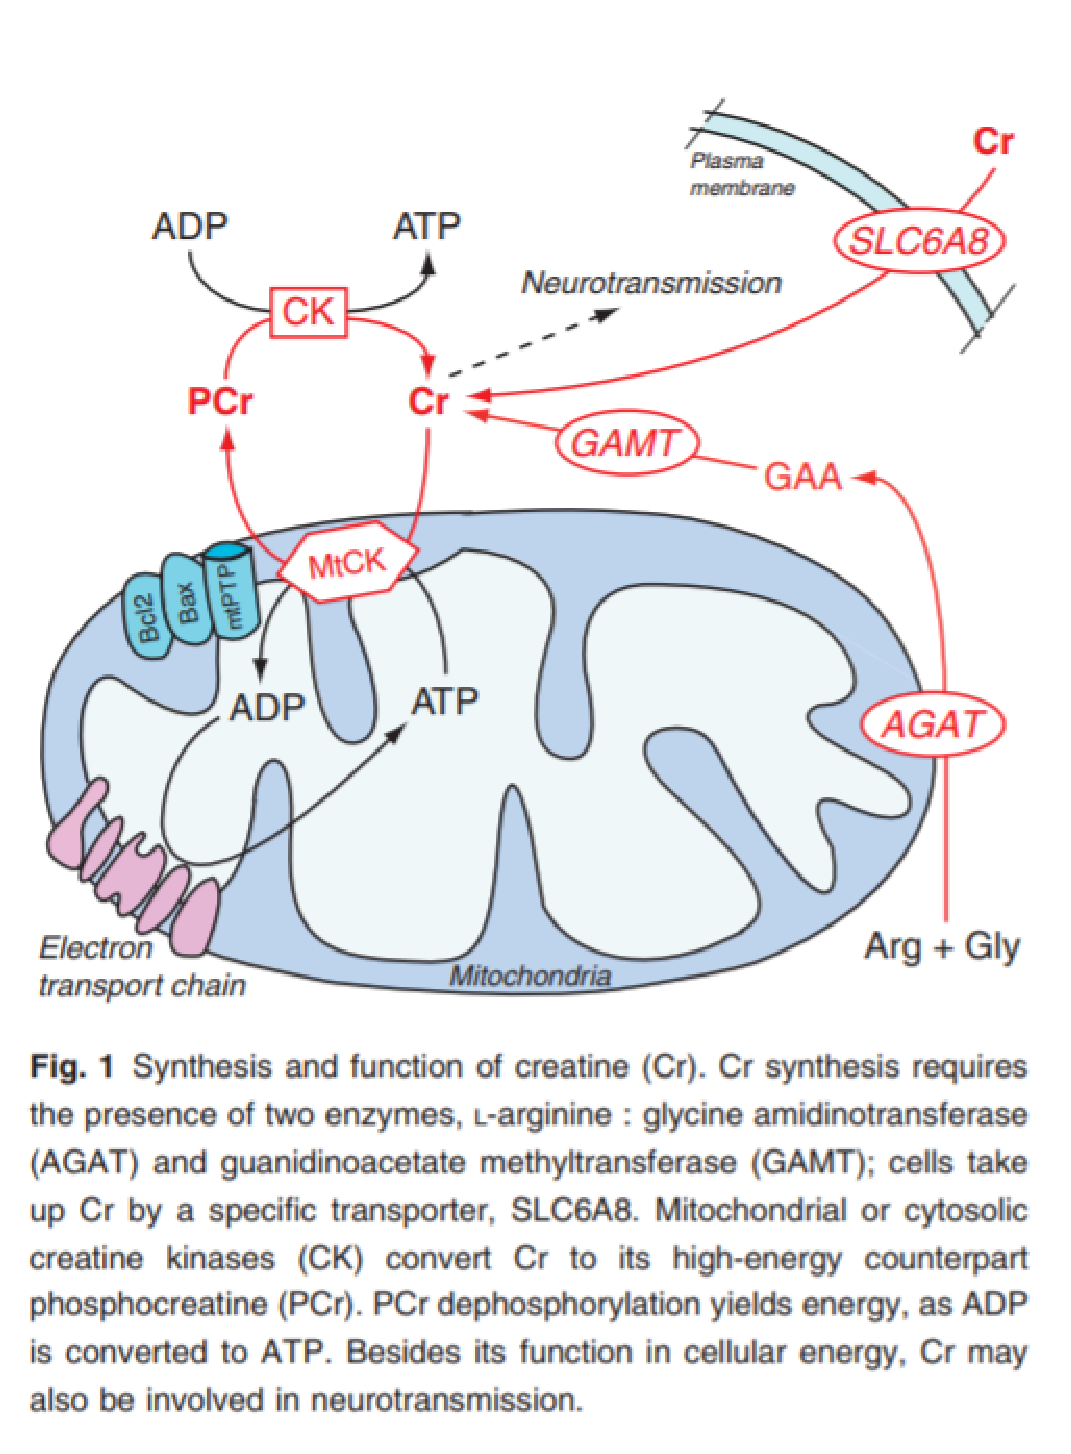
\includegraphics[height=5cm,
    angle=0]{./images/Cr-Pcr-system.eps}}
\caption{Creatine is converted into PCr at two different locations}
\label{fig:Cr-Pcr-system}
\end{figure}

4 CK isoforms, based on tissue expression (muscle vs brain) and subcellular
distribution (cytosol vs. mitochondria) (Beard, Braissant, 2010)
\begin{enumerate}
  \item two cytosolic forms: M-CK (muscle) and B-CK (brain)

  \item two mitochondrial forms: sarcomeric muscle form (sMtCk) and brain form
  called ubiquitous MtCK (uMtCK)


So, creatine can get pass the mito-outer-membrane (MOM) and

\end{enumerate}


Certain cell types also maintain intracellular Cr and PCr pools in addition to
ADP and ATP.  Total Cr (Cr + PCr) in 70 kg young adults amounts for
approximately 120 g. Both Cr and PCr are non-enzymatically and irreversibly
degraded to creatinine at a rate of about 1.7\% of total body pool per day (Wyss
and Kaddurah-Daouk 2000). \textcolor{red}{Creatine degrades spontaneously after
a while to {\bf creatinine} which leaves the cells, enters the bloodstream and
is excreted by the kidneys.} The amount of Cr provided by diet or by endogenous
synthesis depends on creatinine excretion but accounts for about 2 g/ day (Casey
and Greenhaff 2000).

\begin{mdframed}

Creatine is contained in the food we eat, especially in meat.
Creatine is also synthesised in the body, mainly in the kidney and liver. This
is quantitatively more important.
\begin{itemize}
  \item  In human, half of Cr stores originate from food, mainly fresh meat,
  fish and dairy products, while the other half is biosynthesized endogenously through the
AGAT/GAMT pathway.

\end{itemize}

HISTORY:
\begin{itemize}
  \item creatine was first found in meat extract resembling beef broth in first
  half of 19th century.

  \item  phosphocreatine - or creatine with a phosphate group stuck on it - was
  first found a century later, i.e. first half of 20th century (i.e. in 1927 by
  the couple Eggleton and Eggleton)
\end{itemize}
It turned out that creatine and phosphocreatine are part of an intracellular
energy management system.

Around 2.5 million kg of creatine are consumed yearly by athletes in the belief
that it furthers their physical endurance and strength.
\end{mdframed}

Early evidences suggested that creatine is not synthesised in either muscle
cells or neurons, but is rather taken up from the fluid surrounding these cells.
This uptake is effected by a special carrier, the creatine transporter (CreaT or
CRT) called {\bf SLC6A8}. In liver and kidney's cells, creatine is synthesized
from {\bf arginine} by

\begin{itemize}
  \item L-arginine:glycine amidinotransferase (AGAT) or aka GATM
  (Guanidinoacetate N-methyltransferase) - \textcolor{red}{in kidney}

From the precursors arginine (limiting factor) and glycine, AGAT
catalyzes the formation of guanidinoacetate (GAA) and ornithine.


  \item S-adenosyl-L-methionine:N-guanidinoacetate methyltransferase (GAMT) -
  \textcolor{red}{in liver}

GAMT  uses S-adenosylmethionine to methylate GAA, producing Cr and
S-adenosylhomocysteine (Brosnan et al. 2009).
\end{itemize}
AGAT and GAMT expression are positively regulated by growth hormone, thyroid
hormone and sex hormones (Carlson and Van Pilsum 1973; McGuire et al. 1984;
Guthmiller et al. 1994; Lee et al.
1994).

\begin{verbatim}
2-step process:

arginine + glycine ---[ GATM or AGAT]---> guanidinoacetic acid

//NOTE: guanidinoacetic acid is also found in the bloodstream

guanidinoacetic acid + SAM ---[GAMT ]-------> creatine

// guanidinoacetic acid reacts with a methyl group
//    donated by a molecule called SAM
\end{verbatim}

While AGAT and GAMT highest expression is found in kidney and liver,
respectively, they are also found in other cell types (at a lower level).
However, recent data showed that most of other tissues, including the brain,
also express the two enzymes that facilitate creating synthesis - AGAT and GAMT.
\textcolor{red}{IMPORTANT: creatine appears to be far more important for the
brain than for muscle, and that individuals deficient in creatine, suffer from
severe intelligence deficits, speech problems, and epilepsy}.

There is evidence that the permeability of the blood-brain barrier (BBB) for
creatine is limited, suggesting that the brain is dependent on its own creatine
synthesis. So, it is important to understand if and how the  neurons/astrocytes
synthesize creatine.
\begin{enumerate}
  \item using  non-radioisotopic in situ hybridization: Braissant et al. (2001)
  shoed that all cells can synthesize creatine from arginine.
%https://www.ncbi.nlm.nih.gov/pubmed/11165387

  AGAT and GAMT presented an ubiquitous neuronal and glial expression, whereas
  CRT1 was present in neurons and oligodendrocytes throughout the brain, but not
  in astrocytes.

The absence of expression of CRT1 in astrocytes and particularly in those
contacting capillary endothelial cells (BBB) reinforces the idea that under
normal conditions the creatine used by the brain is synthesized mainly in the
CNS.

%  \item
\end{enumerate}




Review: \url{https://www.ncbi.nlm.nih.gov/books/NBK209321/}



\subsection{-- arginine}
\label{sec:arginine}

Arginine is a compound with high energy, i.e. readily to relase a phosphate
group to ADP to form ATP.

Arginine is converted into creatine (Sect.\ref{sec:creatine})
by L-arginine:glycine amidinotransferase (AGAT).

{\it ASS1} gene encodes the rate-limiting enzyme in the urea cycle, the
metabolic pathway responsible for the clearance of nitrogenous waste and the
biosynthesis of arginine (Delage et al., 2010). This seems to be important in
studying cancer (Kremer et al. 2017).
%https://www.cell.com/cell-reports/fulltext/S2211-1247(16)31799-5


\subsection{2.2. Glycolysis: Glycolytic system (16 cal/min): break down glucose
into pyruvate}
\label{sec:glycolytic-system}
\label{sec:glycolysis}
\label{sec:glycolysis-anaerobic}
\label{sec:anaerobic-glycolysis}
\label{sec:ATP-production-in-cytosol-via-glycolytic-system}

If the phosphagen system cannot produce enough ATP
(Sect.\ref{sec:phosphagen-system}), the glycolytic system is the "next in line"
tool that the cell would use and it needs, mainly, glucose
(Sect.\ref{sec:glucose}), which produces Glucose-6P as the first step.
Other sugars that can involve are
\begin{enumerate}
  \item Galactose $\rightarrow$ Glucose-6P (G-6P)

  \item Fructose (from adipose tissue) $\rightarrow$ Fructose-6P (F-6P)
  \item Fructose (from liver) $\rightarrow$  DHAP
  \item Fructose (from liver) $\rightarrow$ GAP
\end{enumerate}
Once getting inside the cell, glucose is converted to Glucose-6P
(Sect.\ref{sec:Glucose-6-phosphatase}), so this is considered as the first step
in glycolysis. NOTE: Glucose is also created inside the cell from stored
glycogen (Sect.\ref{sec:glycogen}).

Like the phosphagen system, oxygen is not required for the actual process of
glycolysis (but it does play a role on the next stage:
aerobically (Sect.\ref{sec:mito_electron-transport-chains}).
Thus, we often see the term {\it anaerobic glycolysis} which refers to true
glycolysis; and {\it aerobic glycolysis} which refers to the truth glycolysis
(in cytosol) + the oxidative metabolism (inside mitochondria).

It is estimated that (fast) glycolysis can create energy at approximately {\bf
16 calories per minute}. In muscle, it is an effective means of energy production
during short, intense exercise, providing energy for a period ranging from 10
seconds to 2 minutes. It is dominant from about 10-30 seconds during a maximal
effort.


% \textcolor{red}{\bf IMPORTANT:} Not all glucose are fully utilized in the
% glycolysis, part of that is converted to lactate (Sect.\ref{sec:lactate}).

\begin{mdframed}
As you can see from glycolysis process, one glucose only generate 2
ATP in the end. This is a pathetic return as in plants, they need to
spend 54 ATP to synthesize one glucose (in {\it Calvin cycle}. In
need, due to the second thermodynamic law, the plant can only create
36-38 ATPs back when convert glucose back to \ce{CO2}. With about 67\%
back, this is indeed very efficient already.
\end{mdframed}

As a result of glycolysis, blood glucose is broken down into  pyruvate, among
other molecules, e.g. ATP, $\ce{H+}$ and NADH
 \textcolor{red}{There are 6 carbons in
glucose, and each pyruvate with 3 carbons.} So, each reaction produces (in net)
\begin{itemize}
  \item 2 ATP molecules,
  \item 2 NADH (Sect.\ref{sec:NADH}),
  \item 2 protons $\ce{H+}$ and
  \item 2 pyruvate$^{-}$  (Sect.\ref{sec:pyruvate})
\end{itemize}
The single glucose molecule only generate 2 molecules of ATP (at the end of
glycolysis). The main focus next is {\bf pyruvate} (Sect.\ref{sec:pyruvate})


\subsection{----- simple form}
\label{sec:glycolysis-simple-form}

Even though the detailed process look quite complicated,
Fig.~\ref{fig:glycolysis}, the overall reaction of glycolysis (occur in the
cytoplasm) is simply as (consider the overal input and final output)

{\tiny
\begin{equation}
  \label{eq:6}
  \underbrace{\ce{C6H12O6}}_\text{glucose} \ce{ + 2 NAD^+ + 2 ADP^{3-} + 2
  HPO_4^{2-} -> 2
  \text{ pyruvate }$^{-}$ + 2 ATP$^{4-}$ + 2 NADH + 2 H$^{+}$ + 2 \ce{H2O}}
\end{equation}
}
Check dibasic phosphate \ce{HPO_4^{3-}} Sect.\ref{sec:dibasic-phosphate}.

Clearly, glycolysis requires the coenzyme \ce{NAD^+} (Sect.\ref{sec:NAD+}),
which requires  lactate dehydrogenase catalyzes the conversion of pyruvate to
lactate in the cytosol, oxidizing NADH to \ce{NAD^+}
(Sect.\ref{sec:lactate-dehydrogenase}).


\begin{figure}[hbt]
  \centerline{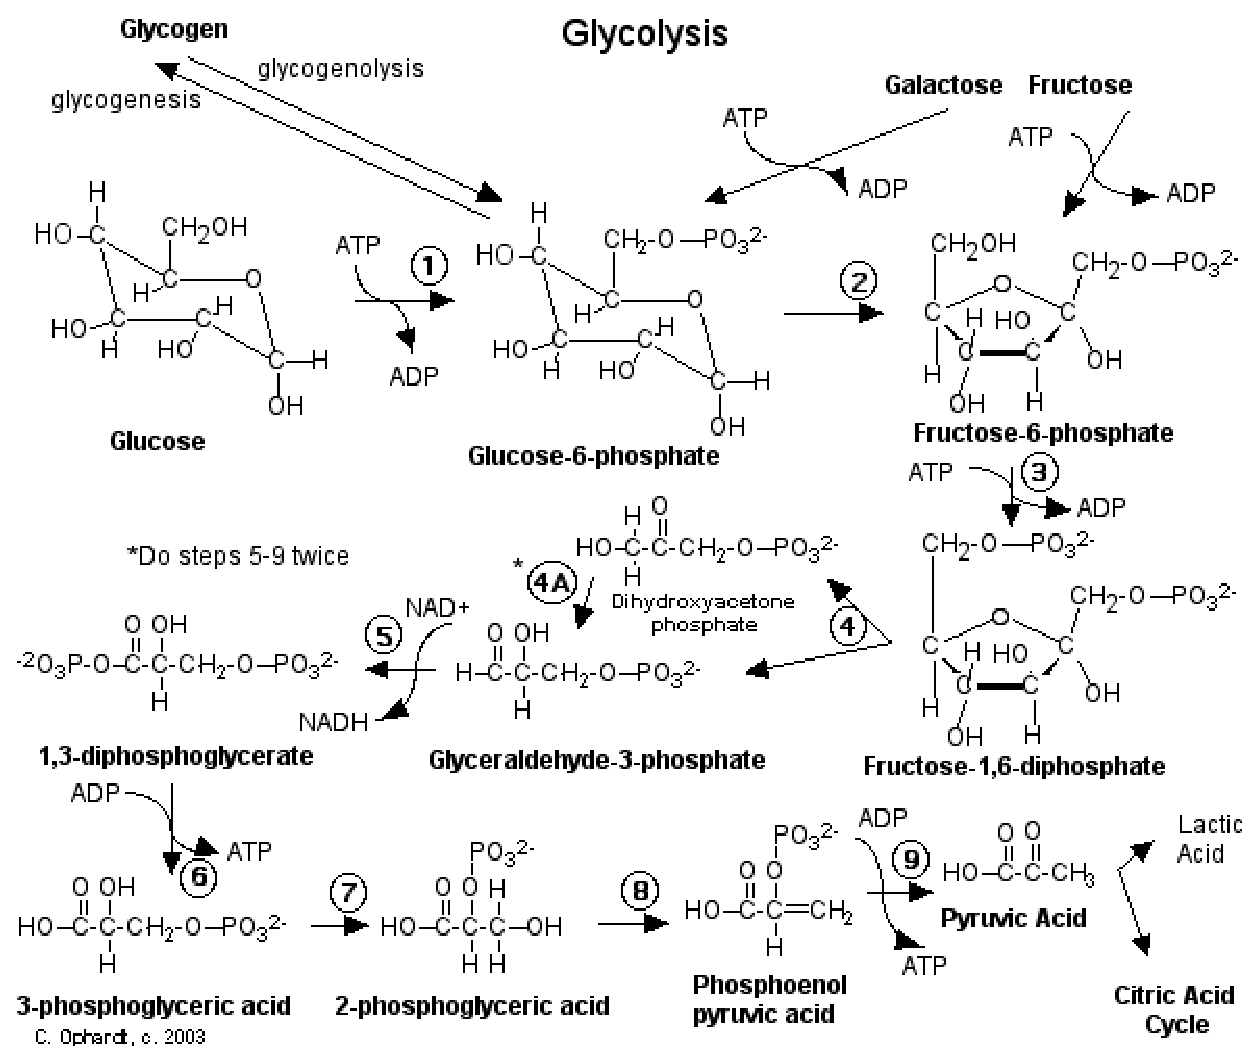
\includegraphics[height=8cm,
    angle=0]{./images/glycolysis.eps}}
\caption{Diagram of glycolysis}
\label{fig:glycolysis}
\end{figure}

% Though there are a variety of starting points for glycolysis, the most
% usual ones are glucose or {\it glycogen}.


\subsection{----- detailed form}

Consider we start with a single glucose molecule

{\tiny
\begin{verbatim}
STEP 1
  Glucose + ATP --[hexokinase, HK]-->   Glucose-6P + ADP
                                        (G-6P)
  G-6P (i.e. G6P) --[PGI]-->   Fructose-6P
                               (F-6P)

  F-6P + ATP <--[PFK]-->    Fructose-1,6-biphosphate + ADP
                            (F1,6BP)
-----------------------------------------------------
  Glucose + 2 ATP  <-------> F1,6BP + 2 ADP

STEP 4+5: 2 products
  F1,6BP     <--[ALDO]-->  DHAP  + GADP
  DHAP       <---[TPI]---> GADP
-----------------------------------------------------


***NOTE:
   G-6P = G6P = Glucose-6P
   F-6P = F6P = Fructose-6P
   F-1,6-BP = F1,6BP = Fructose-1,6-biphosphate
   G-3P = G3P = GADP = glyceraldehyde-3-phosphate
   DHAP = dihydroxyacetone phosphate

(NOTE: after here we have 2 molecules of G3P or GADP)

STEP 6:
2 G3P + 2 NAD+   <---[GAPDH]---->   2 NADH  + 2  1,3BPG + 2 H+

NOTE: 1,3-(bi/di)phosphoglycerate = 1,3BPG

2  1,3BPG  + 2 ADP  <--[PGK]---> 2  3PG  + 2 ATP

NOTE: 3-phosphoglyceric-acid = 3PG

2  3PG   <---[PGM]----->   2  2PG

NOTE: 2-phosphoglyceric-acid = 2PG

2  2PG  <---[ENO]----->  2 PEP

NOTE: phosphoenol pyruvic acid = PEP

2 PEP + 2 ADP -------> 2 pyruvic acid  + 2  ATP
\end{verbatim}
}

\textcolor{red}{Enzymes involve}
\begin{itemize}
  \item HK (hexokinase): step 1
  \item PGI: step 2
  \item PFK
  \item ALDO
  \item TPI
  \item GAPDH : step 6 - Sect.\ref{sec:GAPDH-enzyme}

  \item
\end{itemize}



So, we need two ATPs, and produce 4 ATPs, i.e. overall glycolysis produces 2 ATP
molecules for every glucose molecule.
\begin{enumerate}
\item Even though the overall purpose of the process is to create
  ATP. The process itself also requires ATP (in step 1 and 3) which
  consume 2 ATP molecules

\item Reactions 6 and 9 are coupled to the formation of ATP, each with
  2 ATP molecules.

\item In the end, the net product of ATPs is $(2+2) - 2 = 2$ ATP molecules.

\item Reaction 5 is an oxidation where \ce{NAD^+} removes 2 hydrogens and 2
  electrons to form one \ce{NADH} and one \ce{H+}.

\end{enumerate}

\subsection{----- fast and slow}

\begin{itemize}
  \item  'Fast' glycolysis occurs with intense activity; and pyruvic acid is
  converted to lactic acid and muscle fatigue ensues quickly.

  \item Slow glycolysis is different. Relatively less power is generated, but
pyruvic acid is converted to acetyl coenzyme A (acA), fed through the oxidative
Krebs cycle, more ATP is produced, and fatigued is delayed -
Sect.\ref{sec:krebs-cycle}.

\end{itemize}



\subsection{Stage 3 (aerobic): inside mitochondria - Oxidative system: 10
cal/min}
\label{sec:stage-3}
%\subsection{}
\label{sec:oxidative-system}

Glycolysis, for every glucose molecule, produces 2 ATP$^{4-}$, 2 pyruvate$^{-}$,
and 2 NADH in the cytosol. If oxygen is available, then the free energy
contained in NADH is further released via reoxidization of the mitochondrial
electron chain and results in the release of 30 more mol of ATP per mol of
glucose.

\textcolor{red}{\bf IMPORTANT:} Most of the pyruvate are utilized in Krebs
cycle. However, there is always a conversion from pyruvate to L-lactate,
regardless of the amount of oxygen available
(Sect.\ref{sec:Lactate-production}).


The main location for ATP production is indeed inside mitochondria -
Chap.\ref{chap:mitochondria-cardiac-models}, Sect.\ref{sec:mitochondria-brain}.
This is described in Stage 3 (this section) via 2 pathways
\begin{enumerate}
  \item  {\bf Krebs cycle} or {\bf TCA cycle} (tricarboxylic acid) or
{\bf citric acid cycle} - discussed in Sect.~\ref{sec:krebs-cycle}.


For each acetyl unit is oxidized, 4 pairs of electrons are
transferred, 3 pairs to \ce{NAD+}, and 1 pair to \ce{FAD}.
The coenzymes \ce{NAD+} is reduced into NADH, and giving electron
higher energy for the electron transport reactions
(Sect.\ref{sec:mito_electron-transport-chains}).

  \item Electron Transport Chain - Sect.\ref{sec:mito_electron-transport-chains}

  \item  Beta Oxidation - Sect.\ref{sec:beta-oxidation}
\end{enumerate}
%: The main stage for

\subsection{3.0. intermediate steps}
\label{sec:pyruvate-to-acetyl-CoA}

Intermediate steps link glycolysis (Sect.\ref{sec:glycolysis}) to TCA cycle
(Sect.\ref{sec:TCA-pathway}). It refer to the conversion of pyruvate
(Sect.\ref{sec:pyruvate}), after being transported into mitochondria's matrix,
into acetyl-CoA (Sect.\ref{sec:Acetyl-CoA}) - which is the input of the TCA cycle
(Sect.\ref{sec:krebs-cycle}).

Oxidation of each glucose creates 2 pyruvates; so if we assume all pyruvate
molecules are converted into acetyl-CoA, then two of this will occur per
glucose molecule oxidation. At the end of this intermdiate step: 2 pyruvates
creates
\begin{enumerate}
  \item 2 \ce{CO2}
  \item 2 NADH
\end{enumerate}
NET REACTION:
{\tiny
\begin{equation}
\text{pyruvate} + \ce{NAD^+}   \text{---[Coenzyme-A]-->  acetyl-CoA  +  NADH}
+ \ce{CO2}  ; \Delta G^\circ = -33.5 \text{kJ/mol.}
\end{equation}
}

REMEMBER that pyruvate, while in cytosol, also involve in the formation of
lactate (Sect.\ref{sec:pyruvate}).

The transportation of pyruvate into mitochondria's matrix is discussed in
Sect.\ref{sec:pyruvate-transporter}. Inside the matrix, pyruvate is  converted
to acetyl-coenzyme A (acetyl-CoA) and carbon dioxide by the enzymes in
the pyruvate dehydrogenase complex (PDC) -
Sect.\ref{sec:pyruvate-dehydrogenase-complex}.


% (Swanson conversion) hoax
% https://ratioscientiae.weebly.com/ratio-scientiae-blog/the-perils-of-wikipedia-the-curious-case-of-the-swanson-conversion

It is described as DETAILS:
\begin{enumerate}

  \item Enzyme: E1$\cdot$TPP, with a proton $\H$ required for the
  intermediate to give off \ce{CO2}, Fig.\ref{fig:pyruvate-acetyl-CoA-step1}


E1$\cdot$TPP = pyruvate decarboxylase with TPP
(Sect.\ref{sec:pyruvate-dehydrogenase-complex}) which performs the first two
reactions: (1) decarboxylation of substrate Pyruvate; (2) a reductive
acetylation of substrate lipoic acid. Lipoic acid is covalently bound to
dihydrolipoamide acetyltransferase (E2).

NOTE: Each pyruvate lost one carbon (forming \ce{CO2}) at step 1, and then lost
2 more at the end of the Krebs cycle (Sect.~\ref{sec:krebs-cycle}). In essence,
the glucose is completely oxidized into carbon dioxide $\ce{CO2}$.

\begin{verbatim}
pyruvate ---[E1]---> CO2 + substrate-2
(substrate-1 ~ pyruvate)

substrate-2 ---[E1]---> lipoid-acid
\end{verbatim}
NOTE: The first two reactions (involving E1) is the rate-limiting step

Check the product of (A) in Fig.\ref{fig:pyruvate-to-acetyl-CoA-detail}
\begin{equation}
\begin{split}
&\text{//pyruvate is decarboxylated} \\
&\text{ pyruvate + \ce{H+} --[E1$\cdot$TPP]--> hydroxyethyl-TPP$\cdot$E1 + \ce{CO2}}
\end{split}
\end{equation}

The C2 carbon of TPP performs a nucleophilic attack on the C2 (ketone) carbonyl
of pyruvate. The reactive carbon (between the N and the S of the five membered
ring, Fig.\ref{fig:pyruvate-acetyl-CoA-step1}) of the TPP is oxidized and transferred
as the acetyl group to lipoamide (which is the prosthetic group of the
dihydrolipoyl transacetylase). This forms hydroxyethyl-TPP.
An H+ ion is required for the intermediate to give off CO2.

\begin{figure}[htb]
  \centerline{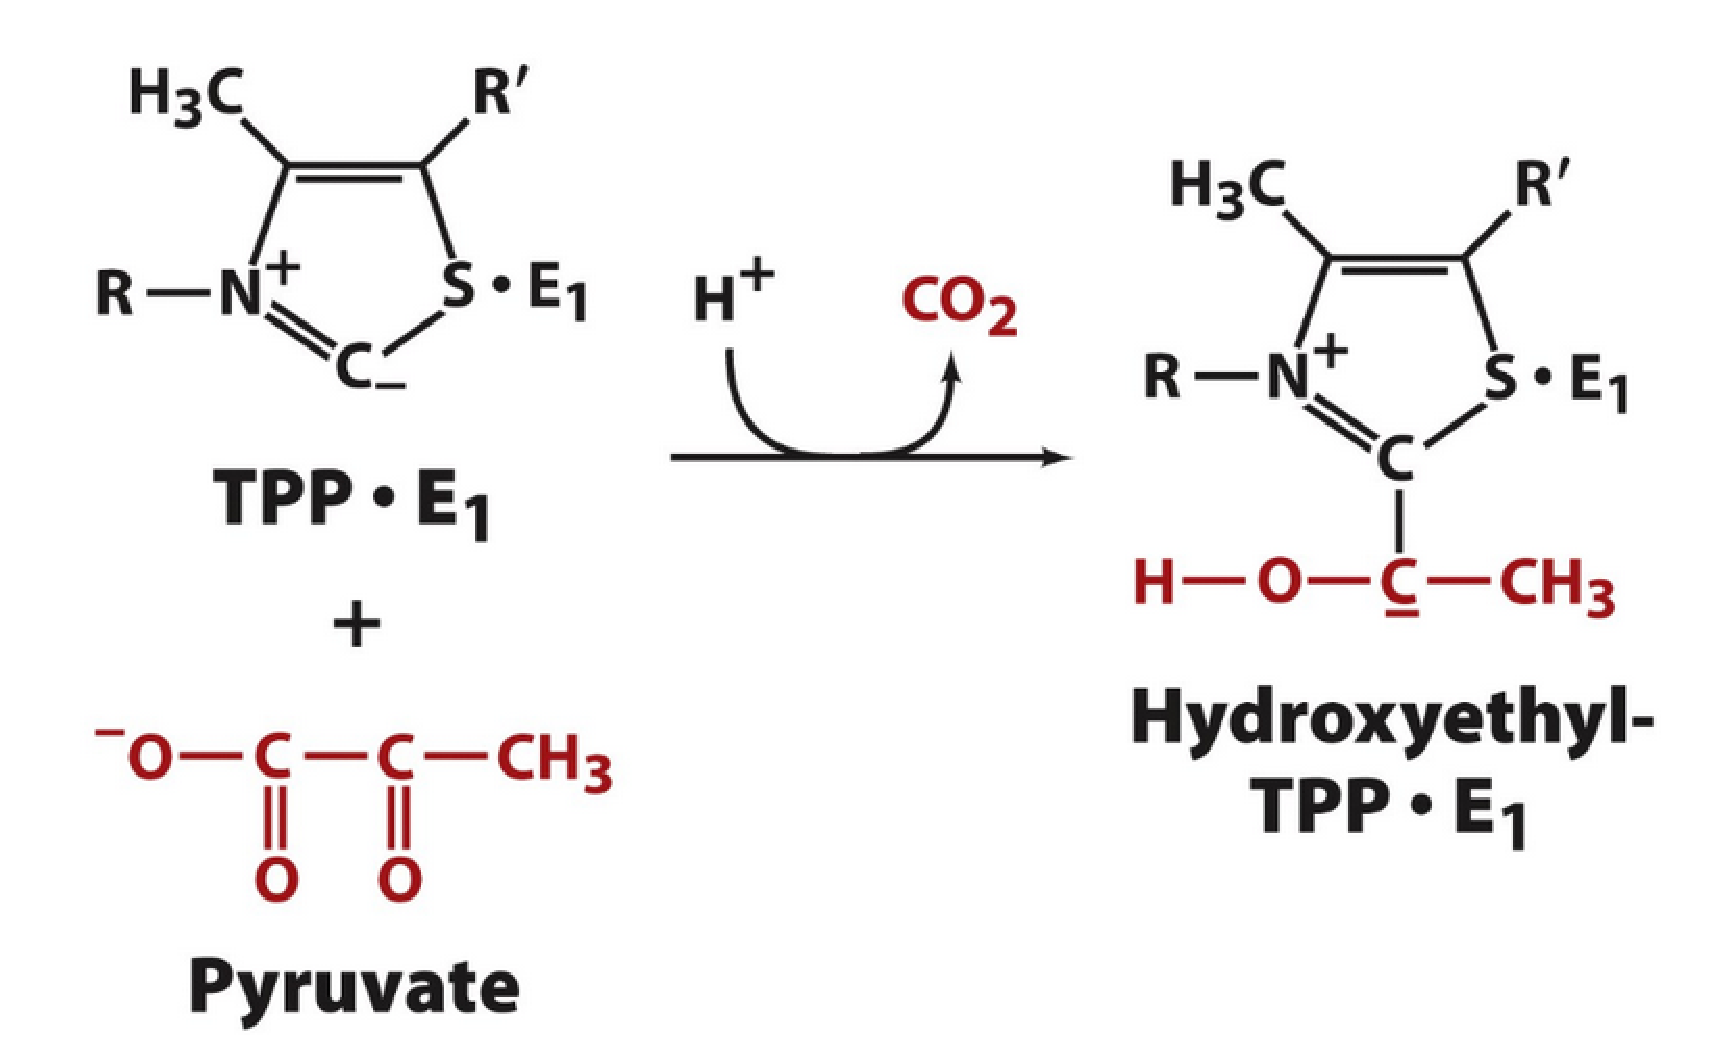
\includegraphics[height=3cm]{./images/pyruvate-acetyl-CoA-step1.eps}}
  \caption{Step 1: pyruvate is decarboxylated by E1 and its prosthetic group
  TPP; with the present of one proton $\H$}
  \label{fig:pyruvate-acetyl-CoA-step1}
\end{figure}

    \item E2$\cdot$lipoamine: oxidizes hydroxyethyl- (of hydroxyethyl-TPP) to
    acetyl- and then transfers acetyl- to CoA

\begin{verbatim}
lipoid-acid + CoA + NAD+ ---[E2]----> acetyl-CoA + NADH
\end{verbatim}

Hydroxyethyl-TPP$\cdot$E1 is  translocated into E2 active site, and is oxidized
by E2, i.e.  the hydroxyethyl- is oxidized into acetyl- and then transferred
to CoA. Check the product of (B, C) in
Fig.\ref{fig:pyruvate-to-acetyl-CoA-detail}
\item
\begin{equation}
\begin{split}
\text{ Hydroyethyl-TPP} + &\text{ coenzyme-A --[E2$\cdot$lipoamine]--->} \\
      &\text{carbanion of TPP + Acetyl-lipoamide}
\end{split}
\end{equation}
This reaction forms acetyl-CoA. However, the process is incomplete.
The E2 is still attached to lysine residue of the acetyl CoA molecule.

The remainder(acetyl group), with two carbons (\ce{C2} fragment), now
attaches to CoA to make Acetyl-CoA.  The \ce{C_2} fragments are reacted with CoA
to form Acetyl-CoA which is the starting point of Krebs cycle.

    \item E3 enzyme is used to oxidizes the thiol groups of the dihydrolipoamide
    back to lipoamide.

At E3 active site, where it undergoes a flavin-mediated oxidation.
As a side reaction, \ce{NAD^+} becomes reduced to NADH.

{\small
\begin{verbatim}
 FAD oxidizes dihydrolipoate back to its lipoate resting state, producing FADH2
 NAD+ cofactor oxidizes FADH2 back to its FAD resting state, producing NADH.
\end{verbatim}
}

REMEMBER that any oxidation reaction needs a coupling reduction reaction.

\end{enumerate}

\begin{figure}[htb]
  \centerline{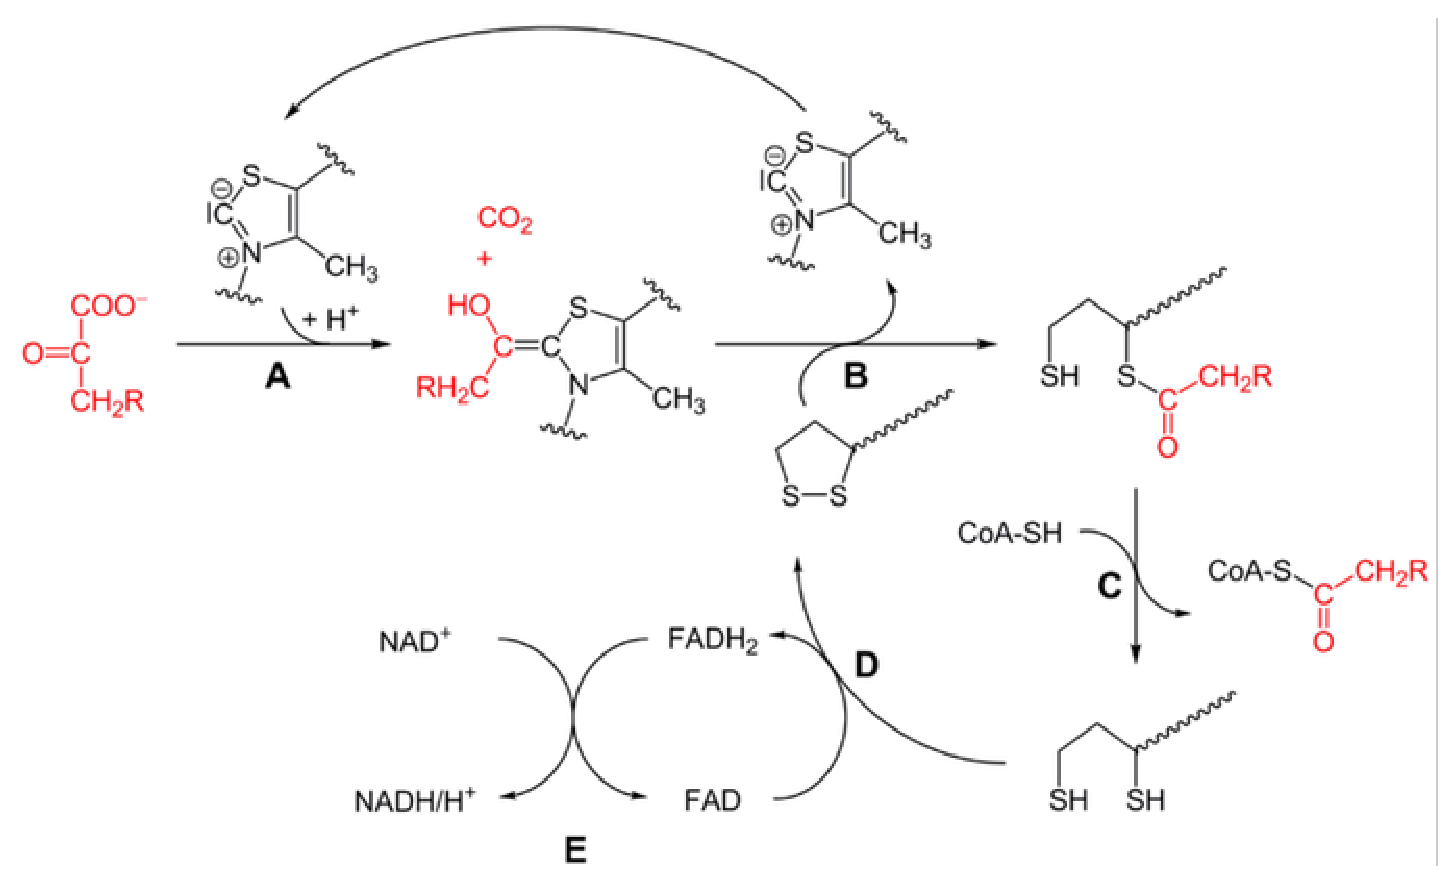
\includegraphics[height=3cm]{./images/pyruvate-to-acetyl-CoA-detail.eps}}
  \caption{Pyruvate to Acetyl conversion}
  \label{fig:pyruvate-to-acetyl-CoA-detail}
\end{figure}

% \begin{equation}
% \begin{split}
% &\text{//pyruvate is decarboxylated} \\
% &\text{ pyruvate --[E1 + TPP]--> acetaldehyde + Glyceraldehyde-3-phosphate}
% \\
% &\text{ acetaldehyde } \ce {<=>[][\text{alcohol dehydrogenase}] }
% \text{ethanol}
% \\
% &\text{ acetaldehyde --[aldehyde dehydrogenase]--> acetate} \\
% &\text{ acetate --[acetyl-CoA synthease (or coenzyme-A)]--> acetyl-CoA}
% \end{split}
% \end{equation}

% The process is described as follows:
% \begin{enumerate}
%   \item {\bf pyruvate decarboxylation} (i.e.
%   remove carboxyl group):
%   the carboxyl group which is fully oxidized (and thus has little chemical
%   energy) is removed and given off as $\ce{CO2}$ molecule.
%
% Here, one molecule of \ce{CO2} is removed from pyruvate and release energy; some
% of which is used to reduce \ce{NAD+} to NADH.
%
% %   \item
%
% \end{enumerate}


\subsection{3.1. Krebs cycle (citric acid cycle, TCA pathway, tricarboxylic
acid cycles)}
\label{sec:krebs-cycle}
\label{sec:citric-acid-cycle}
\label{sec:TCA-pathway}

The {\bf citric acid cycle} (or {\bf tricarboxylic acid} (TCA) cycle or
{\bf Krebs cycle} - as discovered by Sir Hans Adolf Krebs in 1937 - which later
was awarded Nobel prize for Physiology and Medicine in 1953).


At Sheffield University, Yorkshire (1935-54), Krebs measured the amounts of
certain 4-carbon and 6-carbon acids generated in pigeon liver and breast muscle
when sugars are oxidized completely to yield carbon dioxide, water, and energy.
He found, in 1937, {\ig a cycle of chemical reactions} that combines
\begin{itemize}
  \item  the end-product of sugar breakdown - an activated form of 2-carbon acetic acid -
  \item with a 4-carbon axaloacetic acid 
\end{itemize}
to form citric acid.

At the end of the cycle, it regenerates oxaloacetic acid through a series of
intermediate compounds while liberating carbon dioxide; and the electrons
(e$^{-}$).

REMEMBER:
\begin{itemize}
  \item this TCA-cycle process, in prokaryotes, occurs in cytosol.

The citric acid cycle reaction sequence is performed in the cytosol with the
proton gradient for ATP production being across the cell's surface (plasma
membrane) rather than the inner membrane of the mitochondrion

  \item the process, in eukaryotes, occurs inside the fluid-filled matrix
  mitochondria of mammalian cells (Sect.\ref{sec:mitochondria-matrix}).

It is part of the oxidative system (Sect.\ref{sec:oxidative-system}).  The
products of this process are inputs for the next step called ETC - which
produces ATP in the matrix of
mitochondria(Sect.\ref{sec:mito_electron-transport-chains}).

  \item citrate is the ionized form (of citric acid) predominates at biological
  pH (Sect.\ref{sec:citric-acid}).

   \item an important characteristic of TCA cycle is the regeneration of citric
   acid, i.e. citric acid level is preserved.

   \item citrate synthase activity is commonly used as a marker of TCA
   cycle activity.

%   \item
\end{itemize}

% It continues to oxidize the glucose that was initiated during glycolysis.

The starting point of Krebs cycle is acetate - in the form of acetyl coenzyme A
(Acetyl CoA - Sect.\ref{sec:Acetyl-CoA}).

REMEMBER: acetyl CoA is the product from pyruvate (Sect.\ref{sec:pyruvate-to-acetyl-CoA}).
As there are two pyruvate produced for one glucose molecule from glycolysis
(Sect.\ref{sec:glycolysis}), the complete oxidation of one glucose requires 2
turns of Krebs cycle; each one produce
\begin{itemize}
  \item 1 GTP - Sect.\ref{sec:GTP}
  \item 2 \ce{CO2}
  \item 1 \ce{FADH2}
  \item 3 NADH
  \item 3 $\H$
\end{itemize}
So, two Krebs cycles produce
\begin{itemize}
  \item 2 GTP - Sect.\ref{sec:GTP}
  \item 4 \ce{CO2}
  \item 2 \ce{FADH2}
  \item 6 NADH
  \item 6 $\H$
\end{itemize}

\begin{mdframed}
There can be hundreds of Krebs cycle occurring simultaneously in a single
mitochondrion; and there can be hundreds to thousands of mitochondria in a
single cell.

So, for each glucose molecule, from glycolysis to the completion of
Krebs cycles, the outcome is
\begin{itemize}
  \item  4 ATP molecules (2 ATP$^{4-}$ from glycolysis +  2 GTP$^{4-}$ from Kreb
  cycles),

  \item 10 \ce{NADH} (2 from glycolysis + 2 from intermediate steps + 6 from
  Kreb cycle),

  \item 2 \ce{FADH2} and

  \item waste (6 \ce{CO2}: 2 from intermediate steps + 4 from TCA cycle)
\end{itemize}

How can these molecules can involve in the production of ATPs??? We will
focus on NADH and \ce{FADH_2} - which involves in the electron transport chain
(Sect.~\ref{sec:mito_electron-transport-chains}).

\end{mdframed}

NOTE: \textcolor{red}{The two important products of TCA cycle: NADH and \ce{FADH_2} -
will be used as fuel for the next stage} - ETC
(Sect.\ref{sec:electron-transport-chain}).

The fluxes through the TCA cycle ($V_{TCA}$) was studied using $^{13}$C NMR
measurement in the brain by measuring the flow from 1-$^{13}$C glucose to
4-$^{13}$C glutamate (Fitzpatrick et al. 1990) in Shulman's Lab at Yale
University.


%   Fitzpatrick SM, Hetherington HP, Behar
% KL, Shulman RG. 1990. The flux from glu- cose to glutamate in the rat brain in
% vivo as determined by 1H-observed, 13C edited 61. NMR spectroscopy. J. Cereb.
% Blood Flow Metab. 10:170–79


% The energy produced in Krebs cycle, however, is not enough.
% To answer the question how the cell can produce enough ATP, let's look
% at the ins and outs of the Krebs cycle.
% \begin{table}[hbt]
% \begin{center}
% \caption{Ins and Outs in a Krebs cycle}
% \begin{tabular}{cc}
% \hline
% In & Out \\
% \hline\hline
% 1 pyruvate & 1 \ce{CO2} (as waste) \\
% 1 \ce{NAD+} & 1 NADH \\
% 1 CoA & 1 Acetyl-CoA \\
% 1 Acetyl-CoA & 2 \ce{CO2} (as waste) \\
% 3 \ce{NAD+} & 3 NADH \\
% 1 \ce{FAD+} & 1 \ce{FADH2} \\
% 1 ADP & 1 ATP \\
% \end{tabular}
% \end{center}
% \label{tab:InOut_Kreb}
% \end{table}

\subsection{----- detailed form}
\label{sec:krebs-cycle-detailed-forms}

While components of the tricarboxylic acid (TCA) cycle may be used to produce
amino acids, fatty acids, or glucose, the carbons from pyruvate are primarily
converted to carbon dioxide

The Krebs cycle require acetyl-CoA - Sect.\ref{sec:Acetyl-CoA}. This is a closed
loop process, so the end product - oxaloacetate (Sect.\ref{sec:oxaloacetate}) -
is reused for the production of ATP in the next cycle.

STEP 1: conversion of citrate to {\bf isocitrate} and liberation of water
{\tiny
\begin{verbatim}
oxaloacetate + acetyl-CoA  -----[citrate synthase]--->   citrate  + CoA-SH
(4-carbon)     (2-carbon)
NOTE:
   citrate = citric acid  = 6-carbon

citrate  <----> H2O   + cis-Aconitate
NOTE:
   Aconitic acid has two isomers: cis-Aconitate, trans-Aconitate

cis-Aconitate  <--[aconitase]-->    iso-citrate
\end{verbatim}
}

\label{sec:alpha-ketoglutarate}
STEP 2: isocitrate conversion into alpha-ketoglutarate; while reducing
\ce{NAD^+} to NADH
{\tiny
\begin{verbatim}
iso-citrate  +  NAD+   <---[iso-citrate dehydrogenase]--->    oxalosuccinate + NADH + H+
NOTE:
   oxalosuccinate = 4-carbon

oxalosuccinate   ---[Isocitrate dehydrogenase]--->    alpha-Ketoglutarate +  CO2
NOTE: rate-limiting, irreversible stage
     alpha-Ketoglutarate  = 5-carbon
\end{verbatim}
}
NOTE: {\bf iso-citrate dehydrogenase} is activated by $[\Ca]$, and is inhibited
by [NADH] and sucinyl-CoA.

STEP 3: alpha-ketoglutarate conversion to succinyl-CoA by enzyme alpha
ketoglutarate dehydrogenase (Sect.\ref{sec:alpha-ketoglutarate-dehydrogenase complex})
{\tiny
\begin{verbatim}
alpha-Ketoglutarate  +  NAD+ +  CoA-SH  --[alpha ketoglutarate dehydrogenase]-->
                                                  Succinyl-CoA + NADH + H+ + CO2

NOTE: irreversible stage
    Succinyl-CoA  = 4-carbon
\end{verbatim}
}
NOTE: enzyme alpha ketoglutarate dehydrogenase is activated by [$\Ca$] and
[ADP] and inhibited by [NADH].

STEP 4: succinyl-CoA conversion to succinate through a reaction catalyzed by
succinate-CoA ligase, while forming GTP (guanosine triphosphate) or ATP.

{\tiny
\begin{verbatim}
Succinyl-CoA + GDP + Pi  ---[Succinyl-CoA synthetase]--->   Succinate +  CoA-SH  + GTP
\end{verbatim}
}


STEP 5: succinate conversion into fumarate by succinate dehydrogenase, and
reduces FADH to FADH2.

{\tiny
\begin{verbatim}
Succinate + ubiquinone (Q)  --[succinate dehydrogenase]-->  Fumarate + ubiquinol (QH2)
\end{verbatim}
}

STEP 6: fumarate conversion to malate by fumarase

{\tiny
\begin{verbatim}
Fumarate + H2O  ---[fumarase]--->   L-Malate
\end{verbatim}
}

STEP 7 (completing the cycle):  L-malate converted to oxaloacetate, by Malate
dehydrogenase, and reduces \ce{NAD^+} into NADH.

{\tiny
\begin{verbatim}
L-Malate +  NAD+  --[Malate dehydrogenase]-->  Oxaloacetate +  NADH + H+
\end{verbatim}
}


\begin{figure}[hbt]
  \centerline{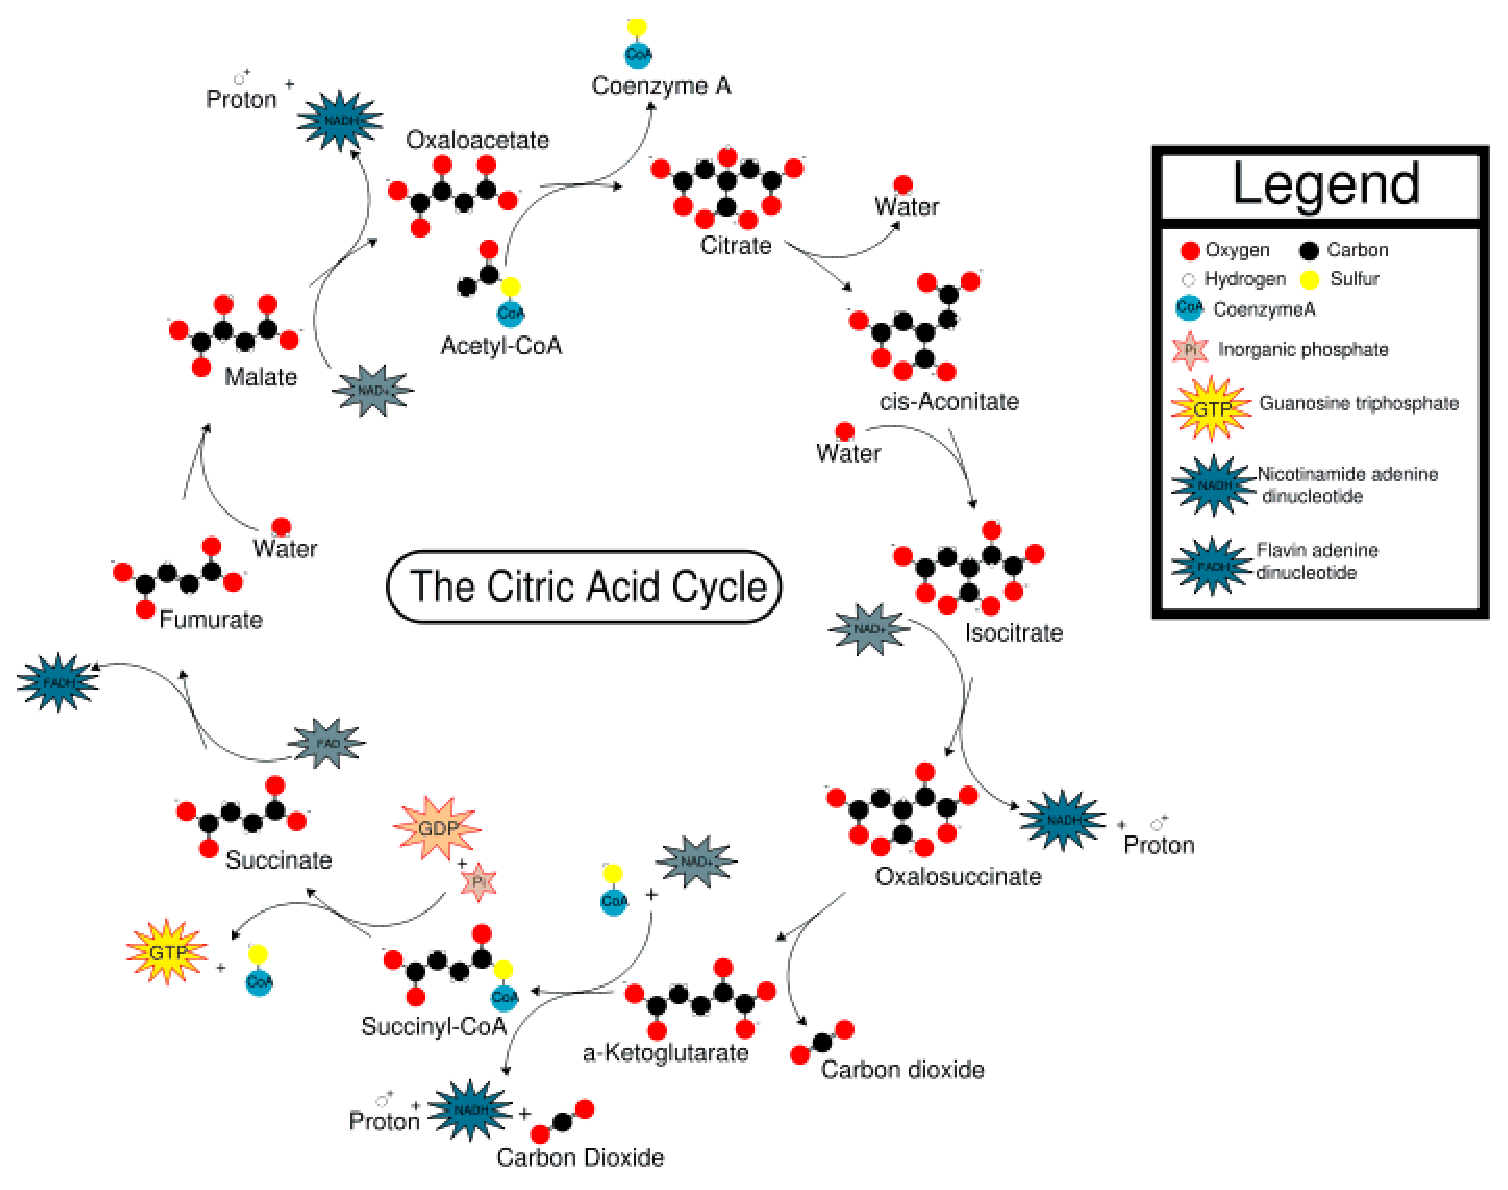
\includegraphics[height=5cm,
    angle=0]{./images/Krebs_cycle.eps}, 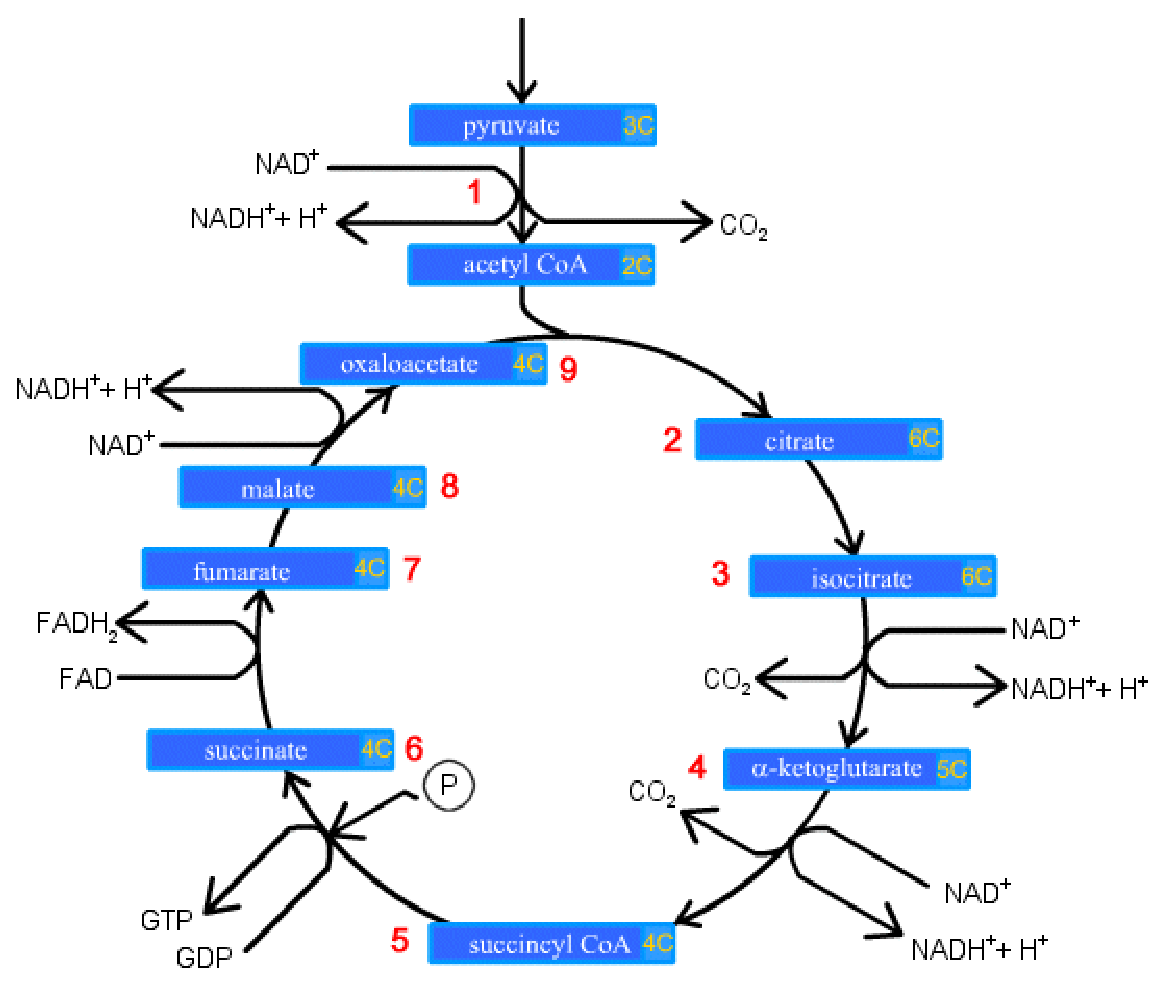
\includegraphics[height=5cm,
    angle=0]{./images/Krebs_cycle_2.eps}}
\caption{Krebs cycle: oxaloacetate - Sect.\ref{sec:oxaloacetate}}
\label{fig:Krebs_cycle}
\end{figure}


% From here, there are two situations: aerobic vs. anaerobic conditions
% \begin{itemize}
% \item In anaerobic condition (no \ce{O2}): NADH cannot be

%   Thus, only 2 ATP are made in the end (similar to above)
% \item In aerobic condition (rich \ce{O2}): NADH can be reoxidized
%   back to \ce{NAD+}by the {\it electron transport chain} (or {\it
%     respiratory chain}).

%   Thus, 6 ATP are made in the end. \textcolor{red}{That explains the
%     essential role of oxygens to the cells}.
% \end{itemize}

\begin{equation}
  \label{eq:10}
  \begin{split}
    \ce{\text{citric acid} -> \text{isocitrate}} \\
    \ce{\text{iso citrate} + NAD+ -> \text{5-carbon molecule} + NADH
      + CO2} \\
    \ce{\text{5-carbon molecule} + NAD+ -> \text{4-carbon molecule} +
      NADH + CO2} \\
    \ce{ADP + \text{4-carbon molecule} -> \text{CoA} +
      \text{succinate} + ATP} \\
    \ce{FAD + \text{succinate} -> \text{funarate} +  FADH2 } \\
    \ce{\text{funarate} ->[hydrolized] \text{malate}} \\
    \ce{NAD+ + \text{malate} -> \text{oxaloacetate} +  NADH } 
  \end{split}
\end{equation}

When Acetyl-CoA enter the mitochondria, Acetyl groups is released and
combine with a four-carbon compound - Sect.\ref{sec:oxaloacetate} - to form
{\it citric acid} (citrate) with 6 carbons (Sect.\ref{sec:citric-acid}).
\begin{enumerate}
  \item a series of chemical reactions to remove 2 carboxyl groups (in the
  oxaloacetate backbone)

The energy generated (from removing carboxyl groups) is in the form of
GTP (or ATP), and as electrons in NADH and QH2 - Sect.\ref{sec:ubiquinol}.

  \item The waste \ce{CO2} is transported back to the blood stream to the lung
  and exhaled.

  \item The 5-carbon molecule is 5-carbon $\alpha-$ketoglutarate.  The 4-carbon
  molecule is {\it succinyl CoA}.

  \item An intermediate in Krebs cycle - succinate - interacts with FAD to
  create \ce{FADH2} which goes to complex II of ETC
  (Sect.\ref{sec:complex-II-mito}); and

  \item the output of Krebs cycle - NADH - goes to complex I of ETC
  (Sect.\ref{sec:complex-I-mito}).

\end{enumerate}


% Sucinate is an intermediate in the citric acid cycle. It serves as an electron
% donor to the ETC
% \begin{verbatim}
% succinate + FAD -> fumarate + FADH2
% \end{verbatim}

\subsection{-- bypass}
\label{sec:krebs-cycle-bypass}

In the citric acid cycle all the intermediates (e.g. {\it citrate, iso-citrate,
alpha-ketoglutarate, succinate, fumarate, malate and oxaloacetate}) are
regenerated during each turn of the cycle.

\begin{itemize}
  \item  the addition of any one of them to the cycle has an anaplerotic effect,
  \item the removal has a cataplerotic effect.
\end{itemize}
This in turn increases or decreases the rate of ATP production by the
mitochondrion, and thus the availability of ATP to the cell.

Oxaloacetate is re-generated; and acetyl-CoA plays the role of fuel, i.e. one
molecule of acetyl-CoA is consumed for every molecule of oxaloacetate present in
the mitochondrial matrix, and acetyl-CoA is never regenerated.


\subsection{-- regulation}
\label{sec:krebs-cycle-regulation}

The regulation of the citric acid cycle is largely determined by product
inhibition and substrate availability.
\begin{enumerate}
  \item Calcium levels -  Sect.\ref{sec:mitochondria-calcium}

$\Ca$ activates pyruvate dehydrogenase phosphatase which in turn activates the
pyruvate dehydrogenase complex whic helps transforming pyruvate to Acetyl-CoA -
Sect.\ref{sec:Acetyl-CoA}.

$\Ca$ activates isocitrate dehydrogenase and $\alpha$-ketoglutarate
dehydrogenase, the rate-limiting step. This increases the reaction rate of many
of the steps in the cycle, and therefore increases flux throughout the pathway.

  \item Feedback inhibition
  \begin{enumerate}
    \item a
  \end{enumerate}
  Feedback inhibition helps to ensure a saturation in production rate, i.e.
  prevents a constant high rate of flux when there is an accumulation of citrate
  and a decrease in substrate for the enzyme.

\end{enumerate}


References:
\begin{itemize}
\item \url{http://www2.nl.edu/jste/aerobic_respiration.htm}
\item \url{http://library.thinkquest.org/C004535/aerobic_respiration.html}
\end{itemize}

\subsection{3.2. Electron transport chains (ETC): respiratory chain}
\label{sec:mito_electron-transport-chains}
\label{sec:electron-transport-chain}
\label{sec:respiratory-chain}
\label{sec:ETC}
% REMEMBER: Glycolysis can produces 2 ATP for each glucose molecule
% (Sect.\ref{sec:glycolysis}); Krebs cycle can produce 2 ATPs for every 2 pyruvate
% output from glycolysis (Sect.\ref{sec:krebs-cycle}).  To meet the energy
% demands, those two processes are not enough.

{\it Electron transport} chain (ETC or respiratory chain) is an important
process of ATP production (Sect.\ref{sec:ATP-synthesis}) in that a flow of
electrons (which carry energies) is coupled to the extrusion of protons $\H$
across the mitochondrial inner membrane (MIM) creating a proton gradient; this
gradient is used to drive ATP synthesis (Sect.\ref{sec:complex-V-mito}).

ETC go through 5 complexes - which are integral components of the inner
membranes, with inputs are NADH and \ce{FADH_2} (Sect.\ref{sec:NADH-FADH2}) at
complex I and complex II. Existence of two separate entry points for electrons
into the ETC ensures a sufficiently active system in case one part is inhibited
without interfering with the other (Tager, Wanders et al. 1983; Balaban and
Heineman 1989; Heineman and Balaban 1990).

\begin{mdframed}
Oxidation of 10 NADH + 2 \ce{FADH2} by oxygen release energy $\Delta G^\circ =
-680$ (kcal/mol) - which is enough to drive the synthesis of several ATPs from
ADPs and P$_i$, knowing that the reaction needs $\Delta G^\circ = +7.3$
kcal/mol.

\textcolor{red}{So, why we still needs ETC?}
The mitochondrion maximizes the production of ATP by transferring electrons from
NADH and \ce{FADH2} through a series of electronc carriers (known as complex I
to complex V) .
Thus, instead of releasing energy at once, this step-by-step transfer of
electron allows the free energy in NADH and FADH2 to be released in small
increments, Fig.\ref{fig:ETC}, electrons traverse through different 'hub' until
it reaches oxygen (at which electron has no further energy).

\end{mdframed}

\begin{itemize}
  \item  At each site during electron transport from NADH to O2,
protons from the mitochondrial matrix are extruded into the
inter-membrane region, which generates a proton concentration gradient
across the MIM.

   \item Each complex comprises a series of redox reactions
(Sect.\ref{sec:redox-reaction}) that involves electron donors and electron
acceptors in the so-called oxidative phosphorylation
(Sect.\ref{sec:oxidative-phosphorylation}).

ETC (electron transport chain) is a spatially separated series of these redox
reactions.

  \item As the electrons move through the chain of proteins, they lose energy, having
little left at its end. Finally, oxygen comes into play, to join with protons
$\H$ and that electron to form water.

\begin{equation}
  \label{eq:7}
  \ce{2 H+ + 2 e+ + 1/2 O2 + ADP -> H2O + 3 ATP}
\end{equation}
This is an exothermic reaction and is just an overall
reaction. Indeed, it requires 8 or more steps.
\end{itemize}


To alleviate this, hydrogen combines with the coenzymes NAD and
FAD (Sect.\ref{sec:NAD}, Sect.\ref{sec:FAD}) and is sent to the ETC.


% \begin{itemize}
%   \item NADH can come from Krebs cycle (Sect.\ref{sec:krebs-cycle}) or (from
%   cytosol) as the result of glycolysis (Sect.\ref{sec:glycolysis-simple-form})
%
%   \item \ce{FADH_2} comes from Krebs cycle only
% \end{itemize}

\begin{mdframed}
NADH and \ce{FADH_2} are energy-rich molecules, i.e. they can readily loosing
electrons (NOTE: NADH has 2 electrons, and FADH$_2$ has ). Electrons from NADH
and \ce{FADH_2} pass through the electron transport chain to oxygen, which is reduced to
water.
\textcolor{red}{REMEMBER the electrons carry energy}. The energy from those
electrons is used to produce ATP.

\end{mdframed}

\begin{figure}[hbt]
  \centerline{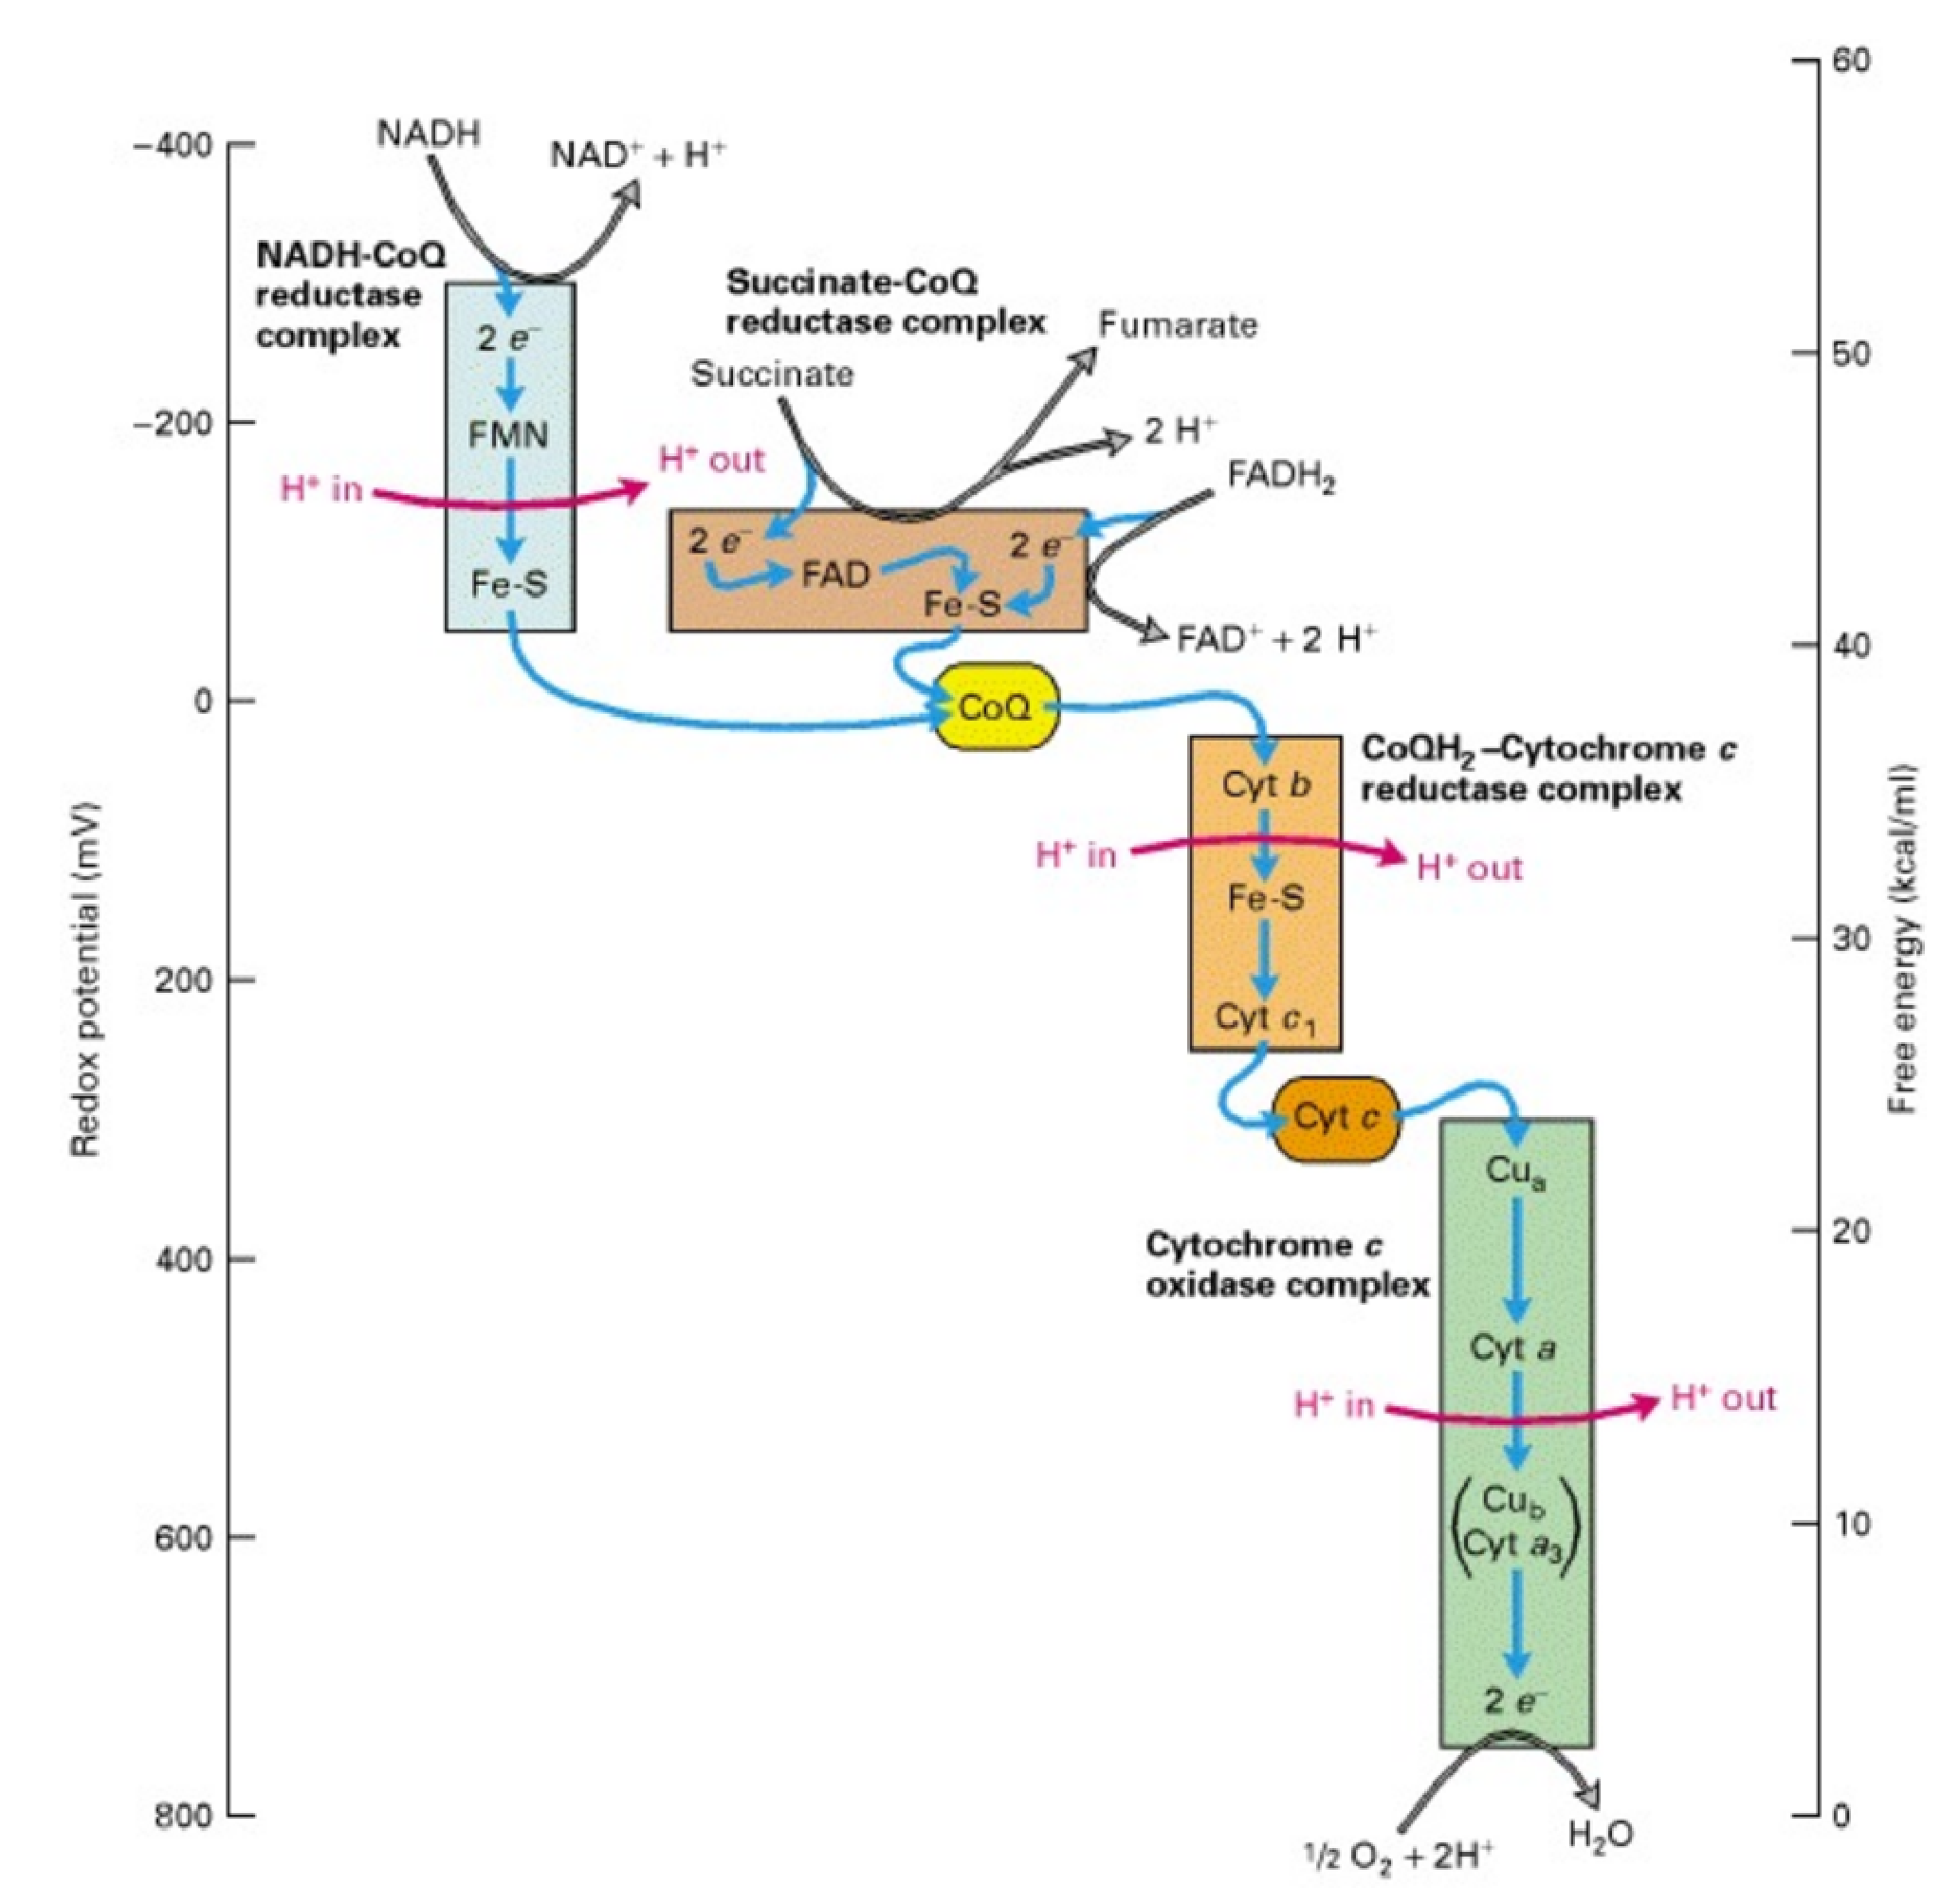
\includegraphics[height=9cm,
    angle=0]{./images/ETC.eps}}
\caption{ETC}
\label{fig:ETC}
\end{figure}

ETC occurs within the mitochondrial inner membrane (MIM) -
Sect.\ref{sec:mito-IMM}. The activities inside the matrix is done either by
soluble proteins or enzymes embedded in the inner membrane.

\begin{mdframed}
ETC is the stage that most of ATP are generated and heavily uses oxygen
(\ce{O2}).  This is why we, and other species, are not able to survive for long
without oxygen. Because of this function, mitochondria are considered as the
power house of cells.

The proton $\H$ produced (in the matrix) during the Kreb's cycle and (in the
cytosol) during glycolysis causes the muscle to become too acidic if not tended
to, which is the major cause of muscle fatigues.  Through more chemical
reactions in the ETC, protons combines with oxygen, {\bf water is produced}, and
acidity is prevented. This process, however, takes time due to the need of
oxygen, which is why the oxidative energy takes a while and intensity of effort
declines.
\end{mdframed}

NADH and \ce{FADH_2} (from the matrix) interact with proteins embedded in the inner
mitochondrial membrane (which we call {\bf proton pumps} (in bacteria) and
{\bf electron transport chains} (in eukaryotes)), losing their electrons to them
in the process. \textcolor{red}{NADH and \ce{FADH_2} are electron donors}.
Passage of electrons between donor and acceptor releases energy,
enables the active process of "pumping" protons $\H$ into the intermembrane
space, i.e. creating $d\Phi$
(Sect.\ref{sec:mitochondria-inner-membrane-potential}).

\begin{enumerate}
  \item NADH release electrons $e^+$ at complex I   -
  Sect.\ref{sec:complex-I-mito}

  \item \ce{FADH_2} release electrons $e^+$ at  complex II -
  Sect.\ref{sec:complex-II-mito}
\end{enumerate}
The output from these two complexes go through the order - complex III
$\rightarrow$ complex IV $\rightarrow$ complex V. These electrons will move
through this series of proteins in the membrane, which make up the electron transport chain.

\begin{mdframed}
Electrons lose energy to power proton pumps, i.e. pumping $\H$ out of matrix
into intermembrane space, against their concentration gradient (i.e. higher $\H$
inner inntermembrane space than that in matrix).
Because of this, a chemical gradient is created because of the high
concentration of hydrogen ions in the inner-membrane space vs. matrix; this
gradient is a store of potential energy
(Sect.\ref{sec:mitochondria-inner-membrane-potential}).

\end{mdframed}

Whenever there's a difference in concentration across a membrane (low $\H$
concentration in the matrix, and high proton $\H$ concentration on the
intra-membrane region), the protons will try to move back to balance the
concentration, to create an equilibrium.
However, the protons can't move freely through the phospholipid bilayer, though
they can cross the membrane through special proteins, e.g. via {\bf ATP
synthase} - Sect.\ref{sec:ATP-synthase}, also facilitating the
creation of ATP, i.e. transforming potential energy to convert (ADP, Pi) into
ATP.


% The ETC process gets its name from the fact that electrons are transported along
% the mitochondria membrane, and in the end to meet up with \ce{O2}, as well as
% producing ATP energy (that we have mentioned in the previous section)

%\textcolor{red}{\bf Inputs to ETC}:



% In mitochondria, during , electrons are transferred from
% electron donors (e.g. NADH) to electron acceptors (e.g. $\ce{O2}$) in the
% so-called {\it redox reactions} (Sect.\ref{sec:redox-reaction}), with the
% transfer of protons $\ce{H+}$ across the inner mitochondria membrane (IMM).
% In eukaryotes, these redox reactions are carried out by a number of protein
% complexes within mitochondria. These linked set of proteins are called {\bf
% electron transport chains}. \textcolor{red}{There are fives main complexes of
% proteins}.


% This process generates electrochemical protein gradient, which is used to
% release energy to form ATP.

\begin{figure}[hbt]
  \centerline{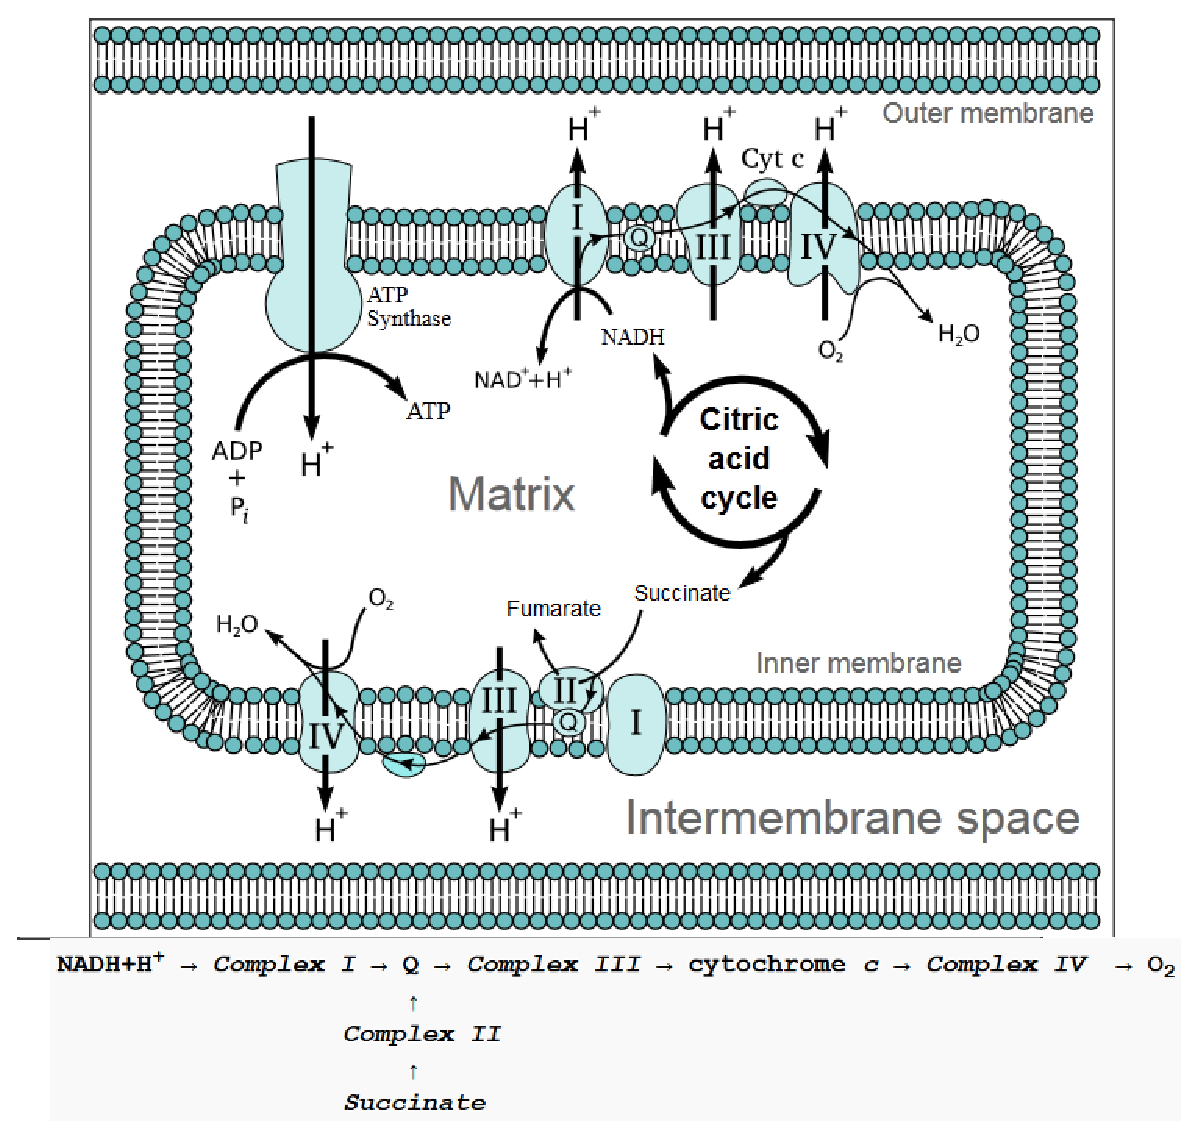
\includegraphics[height=9cm,
    angle=0]{./images/mito_electrontransportchain.eps}}
\caption{Electron transport chain}
\label{fig:mito_electrontransportchain}
\end{figure}

\subsection{--- proton-motive force}
\label{sec:proton-motive-force}

The free energy released during the oxidation of NADH or FADH2 is stored both
as an electric potential and a proton concentration gradient - collectively, the
proton-motive force - across the inner membrane.

The movement of protons back across the inner membrane, driven by this force,
is coupled to the synthesis of ATP from ADP and Pi by Fo/F1-ATPase
(Sect.\ref{sec:Fo/F1-ATPase})

\subsection{--- by products and its diseases}

During this vital process, it also produces harmful {\bf reactive oxygen
species} (ROS), e.g. superoxide ($\ce{O2-}$) and hydrogen peroxide
($\ce{H2O2}$ which is converted from superoxide) - Sect.\ref{sec:ROS}).

Mishandling of superoxides generated by mitochondrial respiratory chain may also
lead to amyotrophic lateral sclerosis (Raha and Robinson 2000; DiMauro and Schon
2003).

\section{-- complex I ({\bf NADH: ubiquinone oxidoreductase}): use NADH and
electrons transfered to Q}
\label{sec:complex-I-mito}

Complex I (NADH:ubiquinone oxidoreductase) is the first site for proton
transportation from the matrix into the inter-membrane space, using the energy
provided by the electron released from NADH, to create the
proton gradient and is the largest multimeric enzyme complex of the
mitochondrial respiratory chain.

\begin{enumerate}
  \item Eukaryotic complex I : has 14 conserved subunits and more than 26
  accessory subunits.

  \item Mammal complex I: has  45 subunits (with a total molecular weight of
  about 980 kDa), which must be assembled correctly to form the properly
  functioning mature complex.
\end{enumerate}


\begin{mdframed}
OVERALL: NADH is oxidized into \ce{NAD+}, and two protons are released into the
inter-membrane space (one taken from the proteon released from oxidation of
NADH, one taken from the matrix by complex I).
Both electron and proton translocation occur simultaneously.

At N module, two electrons are removed from \ce{NADH}, along with the release
of one proton $\H$; both then taken up by prosthetic molecule {\bf flavin
mononucleotide} (FMN). Reduced FMN then passes the electrons to iron-sulphur
(FeS) clusters to ubiquinone - the first electron acceptor, and the two protons
are released into the inter-membrane space. Ubiquinone then carries the electron
to complex III (Sect.\ref{sec:complex-III-mito}).

Complex also absorbs one more proton from the matrix.
\begin{enumerate}
  \item donor: NADH

  \item acceptor: lipid-soluble carrier - ubiquinone (Q) -
  Sect.\ref{sec:coenzyme-Q10} which helps to pass the electrons, with a lower
  energy level now about -50 kcal/mol, to complex III
  (Sect.\ref{sec:complex-III-mito})
  %\item acceptor: Q, with electron of lower free energy level
\end{enumerate}

  \begin{equation}
    \label{eq:12}
%    \begin{split}
      \ce{NADH ->[oxidized] NAD+ + H2 + e(Q)}
%    \end{split}
  \end{equation}

\end{mdframed}

\subsection{structure}
\label{sec:complex-I-structure}


Complex I has two arms, forming an L-shaped structure, with one hydrophobic arm
and one hydrophilic arm.
\begin{itemize}
  \item hydrophilic arm: has 8 subunits (in bacteria Thermus thermophilus)
  comprised the peripheral part of this arm. The peripheral part
  consists of 2 functional modules, an electron input module (N module)
  and an electron output module (Q module)

\begin{enumerate}
  \item {\bf N module}: NADH oxidation site with an FMN molecule as the primary
  electron acceptor

  \item {\bf Q module}: a ubiquinone reduction site.

NADH dehydrogenase (ubiquinone) is the enzyme (located in IMM in eukaryotes)
that catalyzes the transfer of released electrons to complex III.
The reduced product - {\bf ubiquinol (QH2)}, freely diffuses within
the IMM (Sect.\ref{sec:mito-IMM}) and translocate 4 \ce{H+} across the membrane,
thus producing proton gradient, where the electrons is used in Complex III.

\end{enumerate}

  \item hydrophobic (membrane) arm:  the membrane arm or the proton
  translocation module ({\bf P module}) contains the 3 subunits (with around 15
  transmembrane stretches)

  These highly hydrophobic proteins are antiporter-like subunits presumably
  involved in proton-pumping activity, i.e. {\it electron transfer is coupled to
  proton translocation} (though the mechanism - direct association through
  protein binding sites or indirectly through conformational changes of the
  enzyme - is obscure)
\end{itemize}

\subsection{related diseases}

Complex I dysfunction is the most common oxidative phosphorylation (OXPHOS)
disorder in humans and defects in the complex I assembly process are often observed.
It is one of the main sites at which premature electron leakage to oxygen
occurs, thus being one of the main sites of production of superoxide
(Sect.\ref{sec:ROS}).

Malfunction of Complex I is known to be associated with some neuromuscular
diseases including Parkinson's.
%
% , passing from molecule to molecule within the membrane, losing some of its
% energy at each step to activate the molecules which are channels
% pumping \ce{H+} from the matrix into the intermembrane space of the
% mitochondrion. This process then builds up a proton gradient with
% higher concentration in the outer membrane.
%
%  ubiquinol (QH2), freely diffuses within the membrane

\section{-- complex II (succinate dehydrogenase complex): use \ce{FADH_2} and
electrons transferred to Q}
\label{sec:complex-II-mito}

Complex II (Succinate:ubiquinone oxidoreductase, CII)

CII is another entry point of ETC for the transfer of electrons from
\ce{FADH_2} to ubiquinone (Q), where the electrons is also used in Complex III.
However, unlike complex I, there is no proton translocated from matrix into
the inter-membrane space by complex II.
\begin{itemize}
  \item donor: FADH2

  \item acceptor: Q, with electron of lower free energy level about -50 kcal/mol
\end{itemize}

CII is inhibited by oxaloacetate - Sect.\ref{sec:oxaloacetate}.

  \begin{equation}
    \label{eq:12b}
%    \begin{split}
      \ce{FADH2 ->[oxidized] FAD + H2 + e}
%    \end{split}
  \end{equation}

\section{-- complex III: entry points for electrons (Q carries electrons)}
\label{sec:complex-III-mito}

Complex III (ubiquinone:cytochrome c oxidoreductase)

Electrons, carried by ubiquinol (QH2) from CI (Sect.\ref{sec:complex-I-mito})
and CII (Sect.\ref{sec:complex-II-mito}) are subsequently transferred from reduced
ubiquinone (ubiquinol) to CIII.

At CIII, the electrons are separated and then transferred to cytochrome C (Cyt
C), the second mobile electron carrier, to reach complex IV.
The energy of electrons are used to pump proton $\H$ from matrix into the
inter-membrane space.
\begin{enumerate}
  \item donor: Q

  \item acceptor: cytochrome C, with electrons of lower free energy now about
  -30 kcal/mol
\end{enumerate}

\section{-- complex IV (cytochrome C oxidase complex)}
\label{sec:complex-IV-mito}

{\bf Complex IV} (cytochrome c oxidase, CIV): is the large protein,
serving as the last enzyme in the respiratory electron transport chain of
mitochondria.

Its function is reducing \ce{O2} to \ce{H2O} by using the delivered electrons,
i.e. taking up two electron pairs, and more protons are translocated out of the
matrix.

\begin{itemize}
  \item donor: cytochrome C

  \item acceptor: oxygen \ce{O2} and combined with proton in the matrix to form
  water
\end{itemize}


NOTE: Cyclooxygenase-2 (COX-2) is inducible by myriad stimuli. As COX-2 plays an
important role in tumor growth, we were interested in its subcellular location
in cancer cells. The inducible COX-2
\begin{enumerate}
  \item in primary cultured human cells has been reported to
  localize to nuclear envelope, endoplasmic reticulum, nucleus and caveolae.
  
  \item COX-2 inhibition may help with to treat cancer, i.e. re-enable apoptosis
  - a process that is disable in cancer. 
  
  The majority of COX-2 was colocalized with {\bf heat shock protein 60}, a
  mitochondrial protein, in colon cancer (HT-29, HCT-15 and DLD-1), breast
  cancer (MCF7), hepatocellular cancer (HepG2) and lung cancer cells (A549) with
  a similar distribution pattern.
  
  By contrast, COX-2 was not localized to mitochondria in human foreskin
  fibroblasts or endothelial cells; which was confirmed using Immunoblot
  analysis.
  
  However:  Calcium-independent phospholipase A2 was colocalized with heat shock
  protein 60 to mitochondria not only in cancer cells (HT-29 and DLD-1) but also
  in fibroblasts.  
  
HT-29 which expressed more abundant mitochondrial COX-2 than DLD-1 was highly
resistant to arachidonic acid and H2O2-induced apoptosis
\url{https://www.ncbi.nlm.nih.gov/pubmed/15878334}
  \item 
  
\end{enumerate}

\section{-- complex V: ATP synthesis by Fo/F1-ATPase}
\label{sec:complex-V-mito}
\label{sec:ATP-synthesis}

This section describes the final step and directly in synthesizing ATP
molecules. Remember that the ETC (from complex I to complex IV) helps to create
a proton $\H$ gradient across the MIM. 

The protons need to move back into the matrix from inter-membrane space via
Fo/F1-ATPase (or F0F1-synthase or Complex V) whose activity couples to the
synthesis of ATP. The structure of the ATP synthase enzyme has only recently
been worked out (Sect.\ref{sec:Fo/F1-ATPase}).

The transmembrane electrochemical potential is then used to promote the
conformational change of CV, resulting in the generation of ATP by ATP synthase
enzyme.

\textcolor{red}{Location}: In yeast, 60\% of Complex V are in the cristae
membrane while in cardiac mitochondria 94\% are found in the crista (Mannella,
Lederer et al. 2013).

\textcolor{red}{Mechanism of activation}: Upon activation, ATP is created at
Fo/F1-ATPase molecules.
\begin{itemize}
  \item  Fo/F1-ATpase uses a proton gradient (i.e. proton motive force
  generated during protons moving across the MIM from matrix to inter-membrane
  spaces) to drive ATP synthesis by allowing the passive flux of protons across
  the membrane down their electrochemical  gradient
  
  \item It is also believed that F0F1-synthase also needs matrix calcium to be
  activated.
\end{itemize}

\textcolor{red}{Stoichiometry}: how many protons transported to generate one ATP
molecule? There are evidence susggesting that the stoichiometry $n$ varied depending on
system. It was suggested that $n=3$ for mitochondria, and $n=4$ for
chloroplasts.

\begin{equation}
\ce{ADP + Pi + nH^+_p <=> ATP + nH^+_N}
\end{equation}

ATP synthase enzyme is remarkably conserved through evolution. ATP synthase sits
in the membrane of mitochondria, and catalyze the synthesis of ATP from ADP and
phosphate driven by a flux of protons across the membrane down the proton
gradient generated by electron transfer. The flux goes from protochemically
positive (P) size, to protochemically negative (N) side. This reaction is fully
reversible.

From catabolic reaction (Sect.\ref{sec:catabolic-reaction}), one gram of
carbohydrate was oxidized to \ce{CO2} and \ce{H2O}, 4.1 kcal was released. The
values for 1.0g fat or 1.0g protein was 9.1kcal and 4.1kcal, respectively.

ATP is the main energy molecules in cell. ATP synthase enzyme is remarkably
conserved through evolution. ATP synthase sit in the membrane of mitochondria,
and catalyze the synthesis of ATP from ADP and phosphate driven by a flux of
protons across the membrane down the proton gradient generated by electron
transfer. The flux goes from protochemically positive (P) size, to
protochemically negative (N) side. This reaction is fully reversible.

% \begin{equation}
% \ce{ADP + Pi + nH^+_p <=> ATP + nH^+_N}
% \end{equation}
% There are evidence susggesting that the stoichiometry $n$ varied depending on
% system. It was suggested that $n=3$ for mitochondria, and $n=4$ for
% chloroplasts.


\section{Mitochondrial inner membrane potential (d$\Phi$ or $\Delta \Psi$)}
\label{sec:proton-electrochemical-gradient-mito}
\label{sec:mitochondria-inner-membrane-potential}
\label{sec:MIM-potential}

There are hundreds or thousands of mitochondria in the cell
(Sect.\ref{sec:mitochondria}). As discussed in
Sect.\ref{sec:mito_electron-transport-chains}, there exists a transmembrane
proton electrochemical gradient d$\Phi$ as a result of the redox reactions which
occurs in the direction of minimizing Gibbs energy.

An electric potential across the inner membrane also results from the uphill
pumping of positively charged protons outward from the matrix, which becomes
negative with respect to the intermembrane space.

\begin{equation}
-\Csc\frac{d\Phi_m}{dt} = \Jresp + \JFoFz + \Jmcu + \JHleak + \Jncxl + \Jant
\end{equation}
with $\Csc$ is the specific capacitance of mitochondria.

The currents across the IMM include the respiration driven by proton pumps of
the electron transport chain ($\Jresp$), F$_1$F$_0$-ATPase ($\JFoFz$),
mitochondrial calcium unitporter ($\Jmcu$), the proton leak ($\JHleak$), NCXL
($\Jncxl$), and ATP/ADP antiporter ($\Jant$). For modeling purpose, these fluxes
should have a representatioin (either phenomenon or mechanistic) based on
experimental data.

Most of the membrane potential of the mitochondrion is generated by the
electrogenic $\H$ pumps in the motochondria inner membrane.
Electron transport across the IMM create a proton gradient across the IMM, and
generate mitochondrial membrane potential ($d \Phi_m$). This transmembrane
potential gradient is high in the range -160mV to -180mV. The proton gradient
has been estimated to be between 0.1pH to 0.5pH (depending on tissue types and
conditions).

If the mitochondria becomes depolarized, mitophagy can be intiated on that mitochondrion (Sect.\ref{sec:mitophagy}).

%\subsection{mitochondrial current: electron transports}



\chapter{Mitochondrion}


\section{Mitochondrion}
%\section{Introduction}
\label{sec:mito_intro}
\label{sec:mitochondria}

Mitochondria, in Greek means {\it thread grain}, is a cytoplasmic organelle,
Fig.\ref{fig:mitochodnria_electronmicrograph}, with many important functions
(e.g. programmed cell death (apoptosys), cell replication, interact with a
number of cellular regulatory pathways, e.g. glucose sensor in pancreatic
$\beta$-cells), and most important of all, generating the cell's major energy
source (ATP) through a process known as {\bf oxidative phosphorylation}
(Sect.\ref{sec:oxidative-phosphorylation}).

Depending on cell types, each cell may have hundreds to thousands of
mitochondria, with different sizes (Sect.\ref{sec:mitochondrion-size}).
The structure is given in Sect.\ref{sec:mitochondrion-structure}.

Due to having its own genome (Sect.\ref{sec:mito-genome}), historically,
mitochondria were thought to have originated by a free-living bacterium
(particularly $\alpha$-proteobacteria) that was engulfed by another cell, and
end up staying there for the benefit of both, e.g. the host cell profitted from
the chemical energy the mitochondrion produced, and the mitochondrion benefitted
from the cell's protected, nutrition-rich environment surrounding it. This is
called {\bf endosymbosis} (i.e. endosymbiont hypothesis)
\footnote{\url{http://evolution.berkeley.edu/evolibrary/article/_0/endosymbiosis_03}}
which was first proposed by  Lynn Marguli (1970).

However, recent genomics data suggest that maybe mitochondria and the nucleus of
the eukaryotes originated simultaneously from the eukaryotes's cell
\citep{gray1999, gray2001, gray2012}.


Mitochondrial dysfunction have been implicated in a number of diseases due to
lack of energy production, e.g. ischemia (Sect.\ref{sec:heartdisease_ischemia})
and neurodegenerative diseases, e.g. Alzheimer's disease and Parkinson's
disease.

\begin{figure}[hbt]
  \centerline{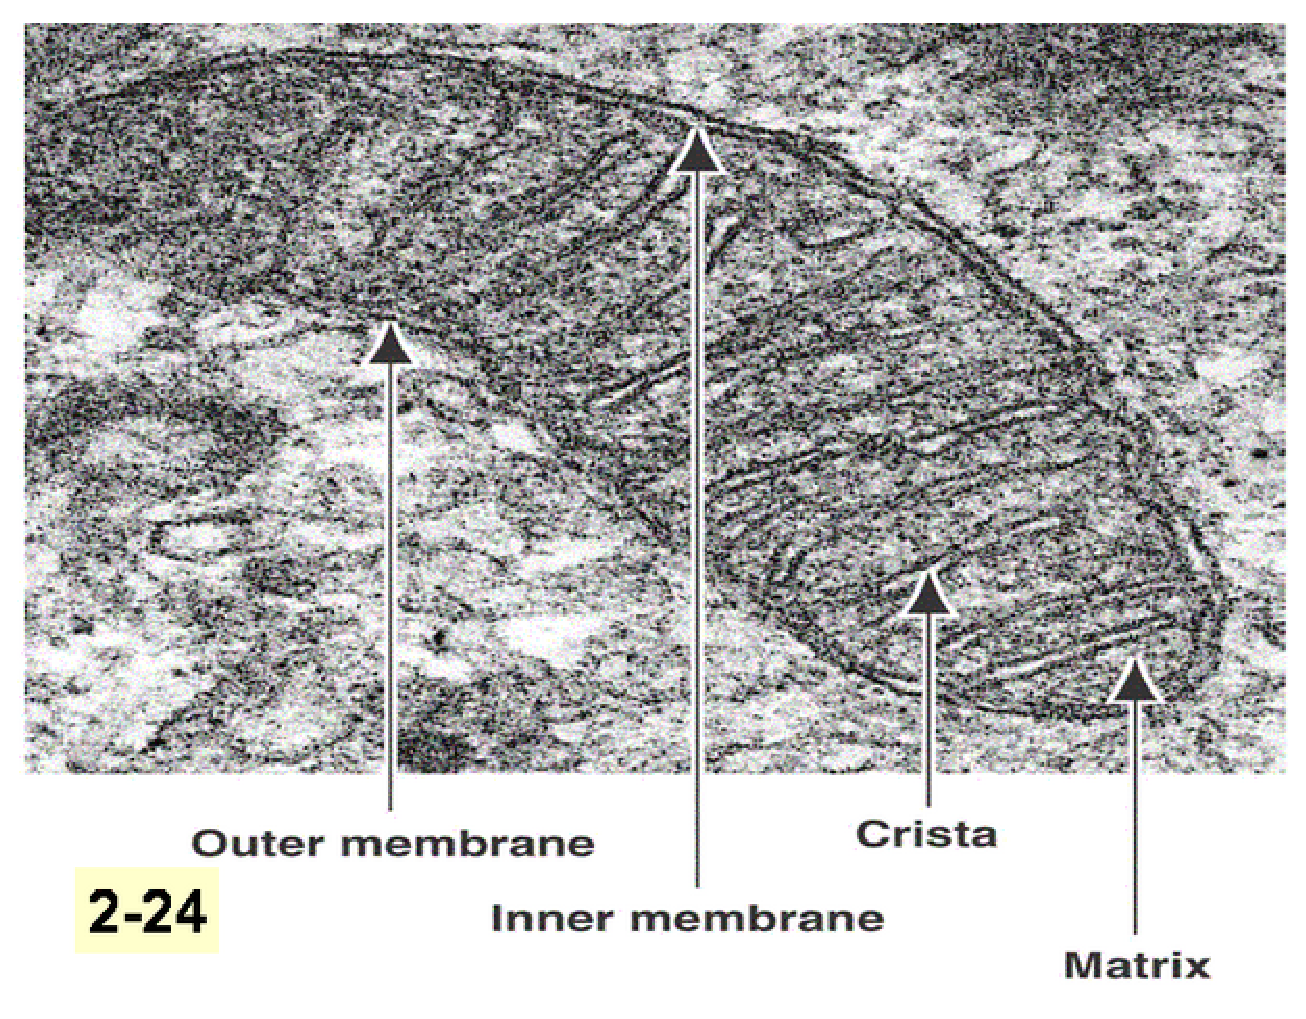
\includegraphics[height=4cm,
    angle=0]{./images/mitochondria_electronmicrograph.eps}}
\caption{An electron micrograph of a liver cell mitochondria at about
20,000-fold magnification
\footnote{\url{http://classes.kumc.edu/som/cellbiology/organelles/mito/}}}
\label{fig:mitochodnria_electronmicrograph}
\end{figure}

\subsection{size}
\label{sec:mitochondrion-size}

The actual diameter of a mitochondrion is about 0.5$\mum$, with 2 membranes
(Sect.\ref{sec:mitochondrion-structure}).

Mitochondrial volume ranged from 0.04-4.26 $\mum^3$ (mean of 1.42 $\pm$ 1.20
$\mum^3$).

In the axonal bouton, percentage mitochondrial volume varied from 6.5\% to 39\%
(mean of 21.3 $\pm$ 7.7\%) (Pierce - Mendell (1993)).

\subsection{mitochondria's marker}
\label{sec:mitochondria-marker}

Citrate synthase (Sect.\ref{sec:citrate-synthase}) is commonly used as a
quantitative enzyme marker for the presence of intact mitochondria.


\subsection{Mitochondria structure}
\label{sec:mitochondrion-structure}


\begin{figure}[hbt]
  \centerline{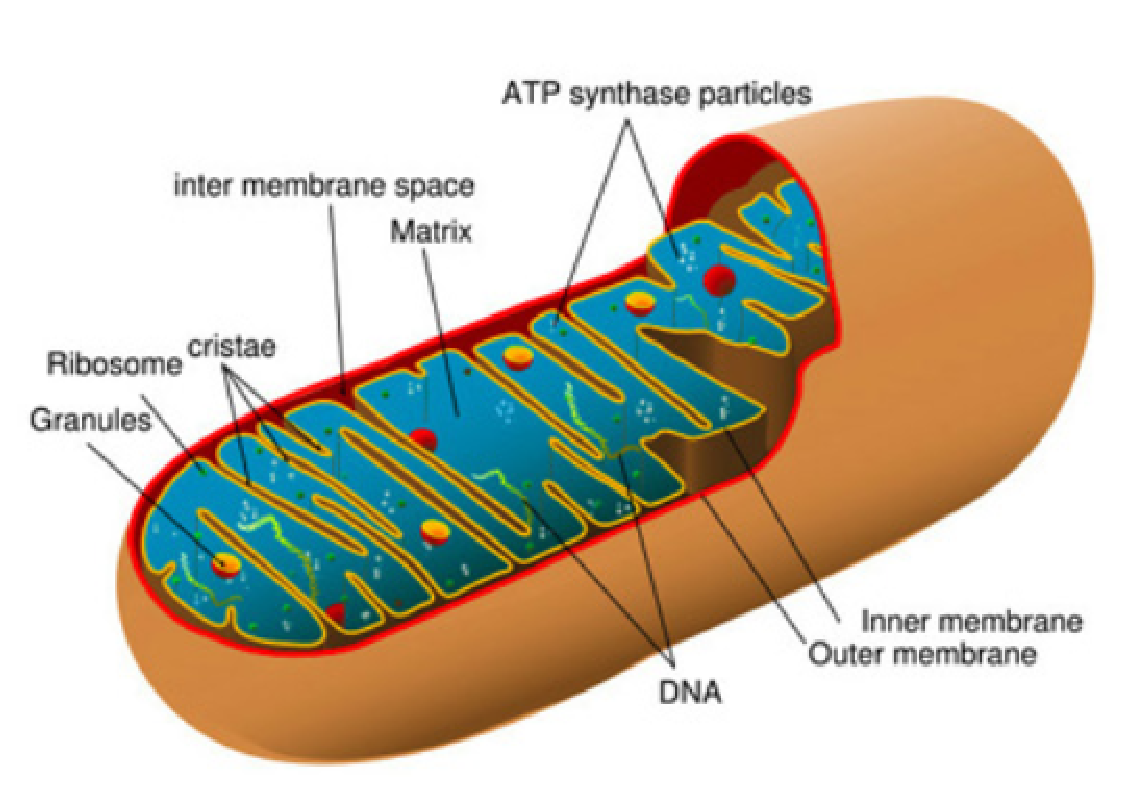
\includegraphics[height=4cm,
    angle=0]{./images/mitochondria.eps},
    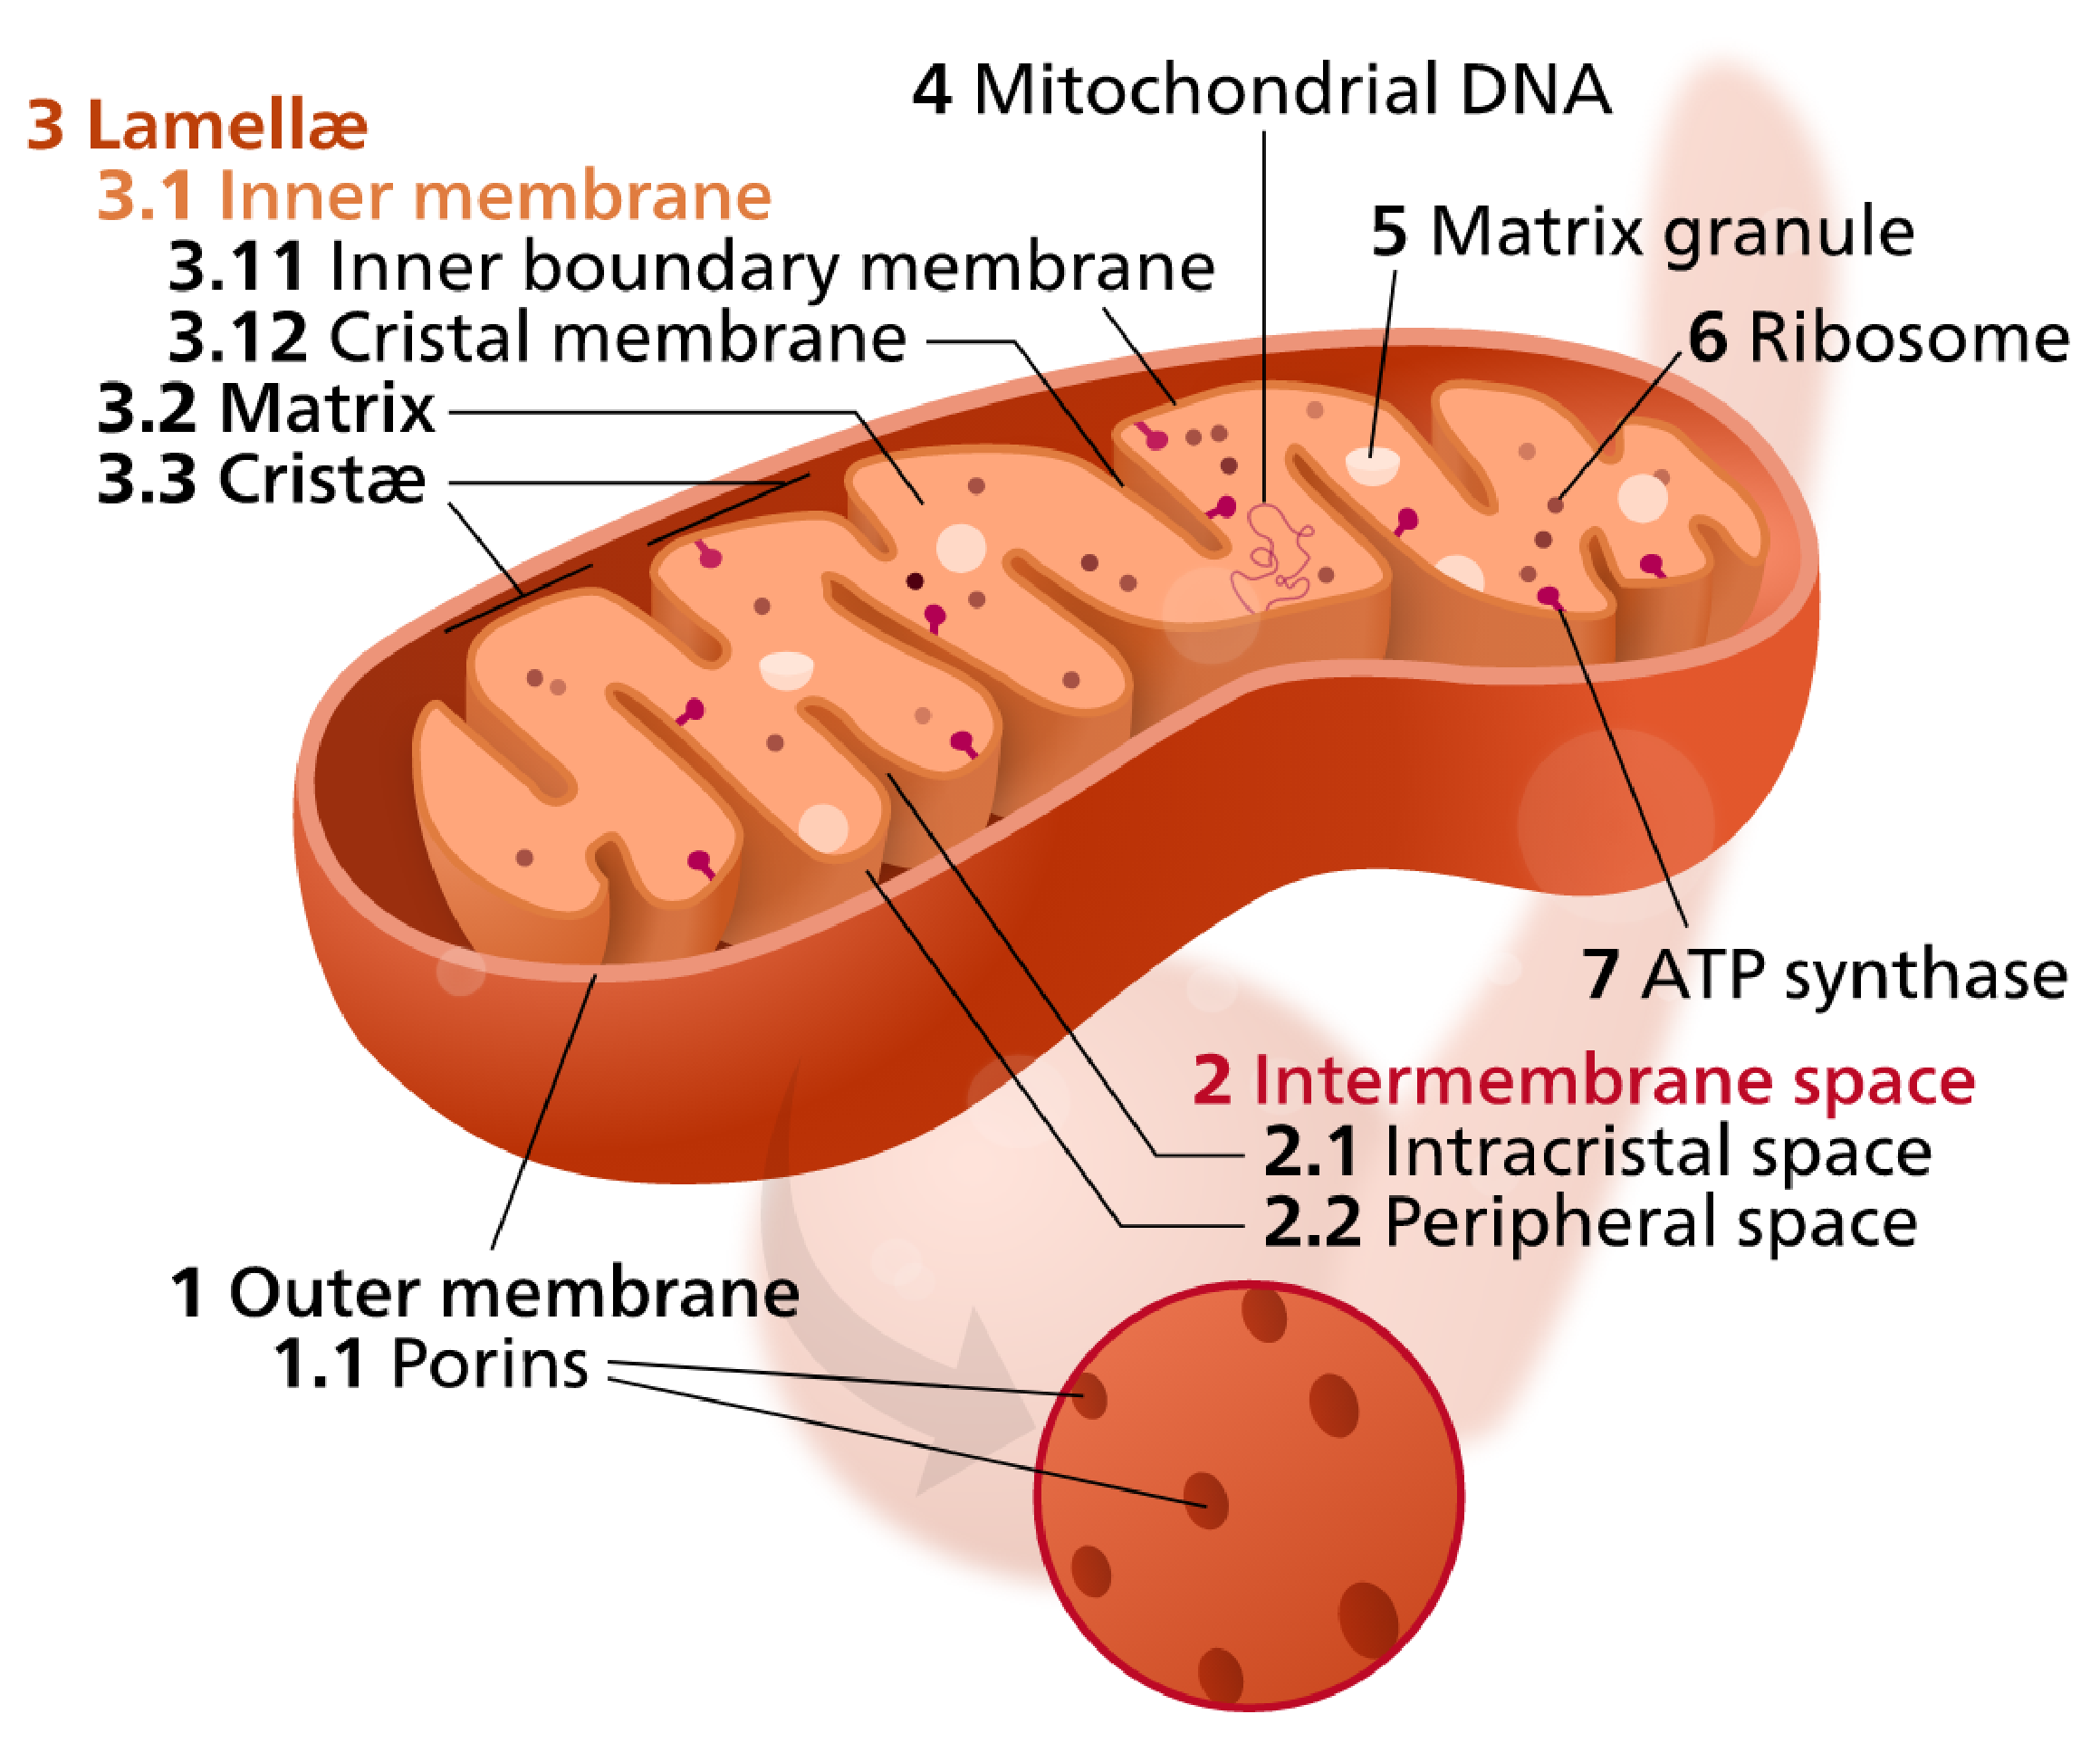
\includegraphics[height=4cm,
    angle=0]{./images/mitochondria2.eps}}
\caption{Mitochondria}
\label{fig:mitochondria}
\end{figure}

The ultrastructure of mitochondria, Fig.\ref{fig:mitochondria}, was discovered
long before the discoveries of the functional differences for different
components \citep{munn1974}.
It has three aqueous components
\begin{enumerate}

  \item the matrix


  \item inter-membrane space (IMS)

\end{enumerate}
divided by two membranes
\begin{itemize}
  \item (mitochondrion) outer membrane (MOM, OMM) - Sect.\ref{sec:mito-OMM}

The volume between the inner and outer membrane is the
intermembrane space.

  \item inner membrane - Sect.\ref{sec:mito-IMM}: the inner membrane heavily
  folding forms cristae-membrane.

\end{itemize}

\subsection{-- inter-membrane space: intracristal space, peripheral space}

NOTE: IMM also fold intensively, creating cristae structure
(Sect.\ref{sec:cristae}).

The intermembrane space between OMM and IMM is called
\begin{enumerate}
  \item The intermembrane space enclosed at two sides by IMM is called intracristal space

  \item	The intermembrane space that is NOT the intracristal space is called
		peripheral space
\end{enumerate}

The molecular composition of this (intermembrane space) region is similar to the
cytosol. This can be attributed to the fact that the OMM is relatively permeable
to molecules less than 1500 Da, compared to that of IMM.



\subsection{-- matrix}
\label{sec:mitochondria-matrix}

NOTE: The inner membrane (IMM) forms tubular and lamellar structures called
cristae (Sect.\ref{sec:cristae}).

The mitochondrial {\bf matrix} is the space found within the IMM.
Mitochondrial matrix houses the enzymes for TCA cycle, mitoDNA, and mitoRNA
among other molecules.

The large surface area of inner membrane facilitates the energy production
occuring at the cristae of the inner membrane, i.e. high protons gradient can be
achieved due to small space.

The movement of \ce{H+} from matrix into the intermembrane space needs to use
ATP as the result of the TCA cycle (Sect.\ref{sec:TCA-pathway}) that occurs
within the matrix.

A series of enzyme complexes on the IMM that functions as proton pumps
(generating the proton gradients), along with the protein complex that uses this
proton gradient as the energy source for producing ATP is called the electron
transport chain (Sect.\ref{sec:mito_electron-transport-chains}). 

Because of that, most chemical reactions occur within the matrix and on the
inner membrane. 

Proteins in the mitochondrial matrix help to carry out
mitochondrial function.


\subsection{- OMM (MOM or OMM)}
\label{sec:mito-OMM}
\label{sec:MOM-mito}

The {\it outer (mitochondrial) membrane} (OM or OMM) or mitochondrial outer
membrane (MOM) is the shell of the organelle, like an eggshell.

What's on the MOM?
\begin{enumerate}
  \item mPTP like TSPO (previously known as the peripheral benzodiazepine
  receptor) - Sect.\ref{sec:mPTP}


  \item
\end{enumerate}

\subsection{- IMM (MIM or IMM)}
\label{sec:mito-IMM}
\label{sec:MIM-mito}

The {\it inner (mitochondrial) membrane} (IM or IMM) or mitochondrial outer
membrane (MOM) is much more complex, with numerous folding (called cristae) and
extremely impermeable; giving it two internal environments: the {\it
intermembrane space} (between IMM and OMM) and the dense 'matrix' (found within
the inner membrane).

\begin{enumerate}
  \item {\bf the inter-membrane space}: the media between the inner and outer
  membranes, and is like the cytoplasm.

  \item {\bf the matrix}: bounded by the inner surface of the inner membrane.
  Its environment is NOT like that of cytoplasm, but is not well-defined. The
  matrix contains  enzyme for TCA cycle (Sect.\ref{sec:TCA-pathway}).
%   \item an inner membrane (IM) surrounding the matrix, which in turn is bounded
%   by an outer membrane (OM).

  \item {\bf cristae} - Sect.\ref{sec:cristae}
\end{enumerate}

MIM is much more restrictive than MOM in terms of permeability (offers selective
permeability to ions and molecules less than 1500 Da.), and transport of these
molecules need to go through certain carriers/channels that exhibit active
transport mechanism, i.e. needs ATP (as produced from TCA cycle).

While the machinery and reactions of the TCA cycle occurring in the
mitochondrial matrix has been studied widely, extent of information on the
various channels located on inner membrane evolved rather gradually.

\begin{enumerate}
  \item mitochondrial pyruvate carriers -  Sect.\ref{sec:pyruvate-transporter}

  \item
\end{enumerate}

Because the outer membrane is freely permeable to protons, the pH of the
mitochondrial matrix is higher (i.e., the proton concentration is lower) than
that of the cytosol and intermembrane space.


Under pathological conditions, mPTP can form - Sect.\ref{sec:mPTP}, breaking
restrictive permeability of MIM and can lead to cell death.


\subsection{** cristae}
\label{sec:cristae}

The folding of the IMM was coined {\bf cristae} (crest) by Palade, providing
high surface:volume ratio.  With high surface:volume ratio, the transport across
the IMM is very high  (Sect.\ref{sec:surface-volume-ratio}).

These crista are non-static structures that change in shape, size and number
depending on energy requirements of the cell during normal physiological and
disease conditions. Thus, it can be established that the morphology of crista
along with the densely packed ATP-producing protein apparatus embedded on it and
the overall mitochondrial function are linked.

During osmotic swelling, the inner membrane can expand and rupture the OMM,
resulting to the loss of mitochondria function. The density of this cristae
structure varied roughly in proportion to the energy demands of the tissues. The
terms 'folds' or 'invaginations' are often used interchangeably to describe
cristae. However, the former one suggest a random, passive adjustment of a
flexible membrane to osmotic pressure or other forces; while the later one a
membrane domain with complex topology and origins \citep{mannella2013}. Thus,
the understanding of how the nano-structure influences the mitochondria function
is still at dawn.


Many proteins reside in the cristae to involve in energy production pathways in
the mitochondria. However, among them, only a few proteins are encoded by
the mitochondrial genome (Sect.\ref{sec:mito-genome}); a larger amount of them
are encoded by genes in the cell's nucleus and transported to the mitochondria via cytosol.

In cardiac cells, the cristae is not merely a random folds of the inner
membrane. Rather, they are distinct, pleomorphic compartments (i.e. having the
ability to alter the shape and size in response to environmental conditions).
These invaginations are connected to the boundary regions of the IM at narrow
circular, or slot-like junctions as small as 10nm \citep{mannella2001}.




\subsection{-- contact site between IMM and OMM}

Another distinct feature of the mitochondria are the specialized 'contact sites'
that are essentially the regions where outer and inner membrane fuse. They are
believed to play an important role in uptake of fatty acids, protein import, and
energy coupling with the cytosol via formation of creatine phosphate (Lesnefsky,
Moghaddas et al. 2001).




\subsection{Mitochondrial genome (mtDNA, mDNA)}
\label{sec:mito-genome}

Mitochondrial DNA (mtDNA or mDNA) is the DNA located in mitochondria.
Due to having its own genome, mitochondria are thought to have originated by a
free-living bacterium (particularly $\alpha$-proteobacteria) that was engulfed
by another cell, and end up staying there for the benefit of both.

% Mitochondrial DNA contains 37 genes, all of which are essential for normal
% mitochondrial function.

The human mitochondrial DNA (mtDNA) is a double-stranded, circular molecule of
16,569 bp (Anderson et al., 1981) and contains 37 	genes coding for two rRNAs,
22 tRNAs and 13 polypeptides
\begin{enumerate}
  \item 13 genes provide instructions  for making enzymes involved in oxidative
  phosphorylation (Sect.\ref{sec:oxidative-phosphorylation}).

  \item remaining genes provide instructions for making molecules called
  transfer RNAs (tRNAs) and ribosomal RNAs (rRNAs) - that help assemble protein
  building blocks (amino acids) into functioning proteins.
\end{enumerate}
In mammalian sperm cells, the copy number of mtDNA is low (50-75), whereas
in mammalian oocytes the copy number is extremely high ($>10^5$). It has been
suggested that, in mammals, mtDNA is only transmitted through the female germ
line \citep{taanman1999}.


\subsection{-- oxidative phosphorylation (OXPHOS): ATP production}
\label{sec:oxidative-phosphorylation}
\label{sec:ATP-production-inside-mitochondria}
\label{sec:OXPHOS}

{\bf Oxidative phosphorylation} (OXPHOS) is the mechanism that cells uses,
occuring inside mitochondria, to produce ATP. As the name suggests, OXPHOS has
an oxidation (of NADH) reaction being coupled to a phosphorylation (of ADP) reaction.
However, remember that for every oxidation reaction, there is always a reduction
reaction (gaining of electrons) that accompanies the oxidation (of NADH).

So, there are 3 separate reactions, eq.\ref{eq:oxphos}

{\tiny
\begin{equation}
\label{eq:oxphos}
\begin{split}
&\text{phosphorylation: }  \ce{ADP^{3-} + HPO_4^{2-} + H^+ -> ATP^{4-} + H2O }
\qquad ; \Delta G^\circ = + 30.5 \text{ kJ/mol} \\
&\text{oxidation: } \ce{NADH -> NAD+ + H+ + 2e^-} \qquad; \Delta G^\circ =
-158.2 \text{ kJ/mol} \\
&\text{reduction: } \ce{ 1/2 O2 + 2H+ + 2e^- -> H2O} \qquad; \Delta G^\circ =
-61.9 \text{ kJ/mol}
\end{split}
\end{equation}
}

The net reaction is obtained by summing the coupled reactions
{\tiny
\begin{equation}
\ce{ADP^{3-} + HPO_4^{2-} + NADH + 1/2 O2 + 2H+ -> ATP^{4-} + NAD+ + H2O}
\qquad; \Delta G^\circ = -189.6 \text{ kJ/mol}
\end{equation}
}

OXPHOS begins with the entry of electrons into the respiratory chain through
Complex I (Sect.\ref{sec:complex-I-mito}) or Complex II
(Sect.\ref{sec:complex-II-mito}).

This pathway is so pervasive that is very efficient in production ATP,
compared to other pathways, e.g. glycolysis (Sect.\ref{sec:glycolysis}).
In mitochondria, this process occurs via the electron transport chains
(Sect.\ref{sec:mito_electron-transport-chains})


Cardiac cells derive the majority of their energy from long-chain fatty acids
and their acyl-CoA equivalents. Cardiac ischemia, as it slows the oxidation of
fatty acids, causes an accumulation of acyl-CoA and induces $\KATP$ channel
opening while free fatty acids stabilize its closed conformation. Reach the
chapter about $\K$ channels in ThermoStat-BioPhysics book to know more about
this type of channel.

[FROM WIKI]:Upon the onset of a cellular energy crisis, mitochondrial function
tends to decline. This is due to alternating inner membrane potential,
imbalanced trans-membrane ion transport, and an overproduction of free radicals,
among other factors. In such a situation, mitoKATP channels open and close to
regulate both internal Ca2+ concentration and the degree of membrane swelling.
This helps restore proper membrane potential, allowing further H+ outflow, which
continues to provide the proton gradient necessary for mitochondrial ATP
synthesis. Without aid from the potassium channels, the depletion of high energy
phosphate would outpace the rate at which ATP could be created against an
unfavorable electrochemical gradient.

\subsection{MICU1}
\label{sec:MICU1}

MICU1 is the calcium sensor that activates the mitochondrial calcium uniporter
(MCU - Sect.\ref{sec:MCU}), and loss-of-function mutations that disrupt this
critical accessory protein result in a disease phenotype characterized by
proximal myopathy, learning difficulties and a progressive extrapyramidal
movement disorder.


\subsection{Mitochondria and Calcium: calcium uniporter (MCU)}
\label{sec:MCU}

MCU is a transmembrane protein located within the mitochondrial inner membrane
and it assembles to form the conducting pore of this highly selective ion
channel. MCU is activated by MICU1 (Sect.\ref{sec:MICU1}).

To help quickly removing $\Ca$ from the cytosol, calcium enters the
mitochondrial matrix through the mitochondrial calcium uniporter (MCU) and other
pathways. Calcium is buffered in the matrix by binding to proteins, ATP and ADP.
This calcium influx is balanced by the extrusion of calcium  out of mitochondria
by NCLX which localize to the cristae (the name NCXL is given due to the fact
that the protein also has $\Li$/$\Ca$ exchange function) \citep{palty2010,
boyman2013}.

The question of how much calcium is sequestered in the mitochondria and the
resulting change in mitochondria is a topic of current debate.  The
interpretation of experiments from different groups suggest either little uptake
of calcium by the mitochondria with a <100 nm change in mitochondrial [$\Ca$]
or a more significant contribution where mitochondrial [$\Ca$] can change
several micromolar.

MCU is voltage-gated and allows unidirectional flow of Ca2+ into mitochondrial
matrix causing depolarization of membrane potential
(Sect.\ref{sec:mitochondria-inner-membrane-potential}).


\subsection{Miro: Miro1, Miro2}
\label{sec:Miro}
\label{sec:Miro2}

Miro is a mitochondrial outermembrane protein with N-terminal contains two
Ca2+-binding GTPase domains (saparated by two EF-hand domains facing cytoplasm -
Sect.\ref{sec:EF-hand-motif}) which with associated proteins, can bind and
control the protein involving in the retrograde and anterograde transportations.

There are two isoforms of miro, classified as miro1 and miro2, which possess a
60\% similarity (Fransson et al., 2003).
Miro1 has been shown to play a role in mitochondrial transport in neurons
(Sect.\ref{sec:kinesin}), but a divergent role for miro2, if any exists, has not
been explored (Niescier, Min, 2013).

Overexpression of the two proteins produce slightly different phenotypes on
mitochondrial morphology: miro1 produces both aggregated and threadlike
mitochondria, while miro2 only generates aggregated mitochondria (Fransson et
al., 2006), suggesting that the roles of miro1 and miro2 are slightly different
on mitochondrial structure.

\subsection{-- Miro1}
\label{sec:Miro1}

Miro1 is one isoform of Miro protein (Sect.\ref{sec:Miro}) and is known as the
primary regulator of anterograde mitochondrial movement along microtubules in
axons and dendrites through an indirect interaction with kinesin-1 heavy chain,
i.e. KIF5B (Tanaka et al., 1998)

The proteosomal degradation of MIRO1 causes kinesin to detach from the
mitochondrial surface, which represents a sophisticated way of putting damaged
mitochondria into quarantine by severing their connection to the microtubule
network before their eventual destruction in the mitophagy process
(Sect.\ref{sec:mitophagy}).


\section{Fussion/Fussion: mitopchondria as a highly connected network}
\label{sec:fission-fusion}

The state of the mitochondrial network is a reflection of the cell’s metabolic
needs under both physiological and stress conditions.

Mitochondria are highly dynamic cellular organelles, with the ability to change
size, shape and position over the course of a few seconds.
In a healthy neuron, fission and fusion balance equally, enabling mitochondria
to form a highly interconnected network.

Mitochondrial shape and structure are maintained by two important but opposing
forces: mitochondrial fission and mitochondrial fusion \citep{reddy2012}:
fission (division of a single organelle into two or more independent structures)
or fusion (the opposing reaction).

These actions occur simultaneously and continuously in many cell types, and the
balance between them regulates the overall morphology of mitochondria within any
given cell.
Fission and fusion are active processes which require many specialized proteins,
including mechanical enzymes that physically alter mitochondrial membranes, and
adaptor proteins that regulate the interaction of these mechanical proteins with
organelles.

The morphology of the mitochondrial network is in a constant state of flux,
influenced by the delicate balance between opposing fusional and fissional
forces.

Although not fully understood, alterations in mitochondrial morphology appear to
be involved in several activities that are crucial to the health of cells.
Unsurprisingly, pathogenic mutations have been identified in several pro-fusion
and pro-fission nuclear genes, with disease phenotypes ranging from severe,
early-onset and invari- ably lethal encephalomyopathies, through isolated optic
atrophy and peripheral neuropathy, to more-complex late-onset multisystemic
neuromuscular disorders.

\begin{enumerate}

  \item In HD:  Defective mitochondrial bioenergetics plays a large role in the progression and
 pathogenesis of HD.

  
Mutant Htt interacts with the mitochondrial protein {\bf dynamin-related protein
1} (Drp1), enhances GTPase Drp1 enzymatic activity, and causes excessive
mitochondrial fragmentation \citep{reddy2012}.

Abnormal mitochondrial dynamics (e.g. increased
fission and decreased fusion) (fission = division of a single mitochondrion into
two, fusion = the integration of 2 mitochondria into a single elongated
mitochondrion).

  \item Mitochondrial dysfunction is a prominent feature of Alzheimer's disease (AD)
neurons. One potential type of dysfunction is redistribution of mitochondria.

  \item 
\end{enumerate}


The main players in this intricate and tightly coordinated process were first
identified in seminal experiments using yeast model, and was found to have been
highly conserved throughout evolution, which is in keeping with the critical
regulatory roles of these proteins in both simple and complex organisms.


\subsection{-- pro-fusion genes: Mfn1, Mfn2, OPA1}

Mitochondrial fusion is controlled by 3 GTPase proteins: 
\begin{itemize}

  \item 2 outermembrane proteins {\bf Mfn1} and {\bf Mfn2}:

\label{sec:Mfn1}
\label{sec:Mfn2}
  The  C-terminal part of Mfn1 mediates oligomerization among Mfn molecules of
  adjacent mitochondria and facilitates mitochondrial fusion.
  
  These two mitofusins are structurally and functionally complementary to OPA1
  and, together, they choreograph a precise chain of mechani- cal events that
  sequentially trigger fusion of the outer, then the inner mitochondrial
  membranes

  \item 1 inner membrane protein
  {\bf Opa1}:
  
  \label{sec:OPA1}
  Following its import into the mitochondrial inter- membrane space, OPA1 is
  first processed by the matrix metalloproteases, which remove the mitochondrial
  targeting signal, and then by proteases of the mitochondrial AAA+ (ATPases
  associated with diverse cellular activi- ties) superfamily, which leads to the
  formation of long and short forms of OPA1. \textcolor{red}{The nature of the
  proteases involved in the maturation steps of OPA1 remains an area of intense
  investigation.}
  
  OPA1 exists as eight isoforms that arise from alternative splicing of exons 4,
  4b and 5b. The cleaving/splicing is done by
  \begin{itemize}
    
    \item  The mitochondrial AAA+ proteases AFG3-like protein 2 (AFG3L2) and paraplegin
  cleave OPA1 at site S1 within exon 5.
  
    \item whereas the ATP-dependent zinc metalloprotease YME1L constitutively
    cleaves OPA1 at S2 within exon 5b

    \item  Other important mitochondrial membrane proteases involved in OPA1
    cleavage include the presenilins- associated rhomboid-like (PARL) protease
    and the metalloendopeptidase OMA1.
  \end{itemize}

  
  OPA1 is firmly anchored, via its transmembrane domain, within the narrow
  junctional regions that insulate the mitochondrial cristae in a zipper-like
  fashion from the rest of the intermembrane space - which is believed to be
  crucial in controlling before cytochrome C is released during apoptosis
  (Sect.\ref{sec:apoptosis-mito}). The TM is followed by a series of coiled-coil
  segments that allow OPA1 to homopolymerize into cylindrical tubular
  structures, which in turn facili- tate the tethering of opposing membranes
  
\end{itemize}
Recently,  a host of equally critical intermediaries are also found
\begin{enumerate}
  
  \item endophilin-B1, 
  
  Endophilin-B1 has also been linked with the regulation of autophagy
  
  \item mito- chondrial fission factor (MFF), 
  
  \item mitochondrial dynamics proteins MID49 and MID51, 
  
  \item mitochondrial protein 18 kDa (MTP18; also known as mitochondrial fission process protein 1), and 
  
  \item mitochondrial fission regulator 1 (MTFR1)
\end{enumerate}

All three main proteins belong to a large family of dynamin-related mechanoenzymes
characterized by a highly conserved dynamin GTPase domain, which is central to
their multifaceted cellular roles and interactions.

Mitochondrial fusion is modulated by the proteolytic processing of two major mediators, OPA1 and MFN2.
Mutations in the pro-fusion genes optic atrophy 1 (OPA1) and mitofusin 2 (MFN2)
were initially reported in families with autosomal dominant optic atrophy (DOA;
OMIM \#605290) and axonal Charcot–Marie–Tooth disease type 2A (CMT2A; OMIM
\#609260), respectively.
\begin{enumerate}

  \item The degradation of MFN2 through ubiquitination is dependent on
  PTEN-induced putative kinase 1 (PINK1, also called mitochondrial
  serine/threonine-protein kinase PINK1), and this process is tightly linked to
  the loss of mitochondrial membrane potential and the autophagic process

  
\end{enumerate}


  
  Although the precise mechanisms still need to be elucidated, both OPA1 and
  MFN2 are involved in the regulation of mitochondrial respiratory chain
  coupling and oxidative phosphorylation (Sect.\ref{sec:respiratory-chain}).
  Fibroblasts from patients harbouring pathogenic OPA1 or MFN2 mutations exhibit
  a mitochondrial coupling defect with reduced mitochondrial membrane potential
  and impaired ATP synthesis.
  
  \begin{itemize}
  
    \item MFN2 is also thought to exert a direct influence on mitochondrial
    biogenesis by regulating the expres- sion of nuclear-encoded respiratory
    chain subunits.
    
    A serious biochemical defect in the visual cortex was observed in MFN2
    mutation carriers with impaired vision secondary to optic atrophy.
  
    \item Impaired oxidative phosphorylation has been found consistently with
    the use of in vivo phosphorus magnetic resonance spectroscopy in the calf
    muscle of patients harbouring a broad range of OPA1 mutations.
    
    
    direct experimental evidence that OPA1 regulates the assembly and
    stability of the respiratory chain supercomplexes through its influence on
    remodelling of mitochondrial cristae.
    
    Recent data also suggest that proteolytic activation of OPA1 is sufficient
    to stimulate mitochondrial inner membrane fusion in a process that is
    sensitive to the oxidative phosphorylation output from the mitochondrial
    respiratory chain.
    These elegant tuning mechanisms ensure a close match between mito- chondrial morphology and the energetic demands of the cell.
    
  \end{itemize}
  
  
  MFN2 is an outer mitochondrial membrane protein but, unlike MFN1, it is also
  enriched at the interface between the endoplasmic reticulum and the
  mitochondria (Sect.\ref{sec:mito-ER-interface}).
  Ablation or silencing of MFN2 disrupts endoplasmic reticulum morphology and
  loosens the interactions with mitochondria, thereby reducing the efficiency of
  mitochondrial calcium uptake in response to stimuli that generate
  inositol-1,4,5-trisphosphate.
  
  The current genetic and biochemical evidence supports a model in which MFN2 on
  the endoplasmic reticulum acts as a structural bridge by engaging in homotypic
  and heterotypic complexes with MFN1 or MFN2 located on the outer mitochondrial
  surface.
  
  MFN2 (on OMM) is thought to play a role in mitophagy (Sect.\ref{sec:mitophagy}). The
  phosphorylated form of MFN2 is thought to be a highly effective receptor for
  parkin, which then undergoes a conformational change to its active form, in
  addition to being drawn into close juxtaposition with PINK1 on the outer
  mitochondrial membrane.
  

\subsection{-- pro-fission genes}

 Mitochondrial fission is regulated by 3 proteins (if we consider in plants,
 then the third Mff is replaced by ELM1 - so in total, we have 4 proteins)
\begin{itemize}

  \item  mitochondrial fission 1
  ({\bf Fis1}) and 
  
  Fis1 is an adaptor protein located in the outermembrane of mitochondria (OMM),
  where it is anchored by a C-terminal transmembrane domain.
  The remainder of Fis1 consists of protein–protein interaction sites which protrude into the cytosol.
  
  \item {\bf Drp1} (aka DLP1).

Drp1 is localized in the cytoplasm,  from where it shuttles back and forth to the OMM during fission events.

With a small part of Drp1 localized to the outermembrane, it promotes
mitochondrial fragmentation. Drp1 interacts with Fis1 at fission sites, where it
is proposed to form a collar that encircles the mitochondrion. The Drp1 collar
tightens around the mitochondrion, and this constriction leads to a severing of
the OMM and fission into two independent organelles.

In yeast, this interaction between DRP1 and Fis1 is mediated by a second set of
adaptors, Mdv1 and Caf4, which can bind both Fis1 and Dnm1 to allow their
association.  Loss of either Fis1 or Mdv1, and to a lesser extent Caf4, prevents
Dnm1 from associating with the mitochondria, and hence blocks mitochondrial
division.

In mammals there is no homologue of Mdv1 or Caf4, therefore the association
between Fis1 and Drp1 at the outer membrane may be more direct, as evidenced by
their ability to bind in vitro.


   \item Mff is a second OMM protein (also found in humans), which is anchored
   at its C-terminus like Fis1. Loss of Mff blocks mitochondrial fission;
   however, its mode of action, and whether it interacts with Drp1 to aid
   fission, is currently unknown.
   
   Mff was discovered in an RNAi screen for mitochondrial morphology mutants in
   Drosophila, and the human protein retains the same function.
   Knockdown of Mff protein levels by RNAi leads to an elongated mitochondrial
   network.
   However, in vitro studies show that Mff is found in a different complex to
   both Fis1 and Drp1, indicating that it may affect mitochondrial fission
   through some unknown pathway.
   
   
   \item (in plants only) In plants (which, like mammals, have Fis1 and Drp1
   proteins but no Mdv1 or Caf4 homologues), ELM1 is localized to the OMM.
   Mutations in ELM1 lead to a decrease in mitochondrial fission, and the
   appearance of elongated mitochondrial tubules with many constrictions,
   indicating that division is blocked after the early events have taken place,
   but before final scission [21]. This was confirmed by the finding that in
   wild-type plants, the dynamin homologue was found at mitochondrial fission
   sites, while it remained in the cytosol in ELM1 mutants, indicating that ELM1
   is required for the mitochondrial placement of dynamin [21]. It remains to be
   determined whether ELM1 acts in a manner analogous to Mdv1 (i.e. bridging the
   gap between Fis1 and dynamin), or whether ELM1 recruits dynamin to fission
   sites directly.
   
\end{itemize}

What regulates the site of fission, and how fission of the IMM is carried out, is currently unknown.
It is suggested that it is near ER-mito interface (Sect.\ref{sec:mito-ER-interface}).


Levels of DLP1 (also referred to as Drp1), OPA1, Mfn1, and Mfn2 were
significantly reduced whereas levels of Fis1 were significantly increased in AD.
Investigating the changes in the expression of mitochondrial fission and fusion
proteins in AD brain and the potential cause and consequence of these changes in
neuronal cells showed that, by mimicking these expresional changes
\begin{itemize}
  \item  caused a similar abnormal mitochondrial distribution pattern, such that
  mitochondrial density was reduced in the cell periphery of M17 cells or
  neuronal process of primary neurons and correlated with reduced spine density
  in the neurite  
  
  {\bf DLP1 overexpression}, likely through repopulation of neuronal processes
  with mitochondria, {\it prevented ADDL-induced synaptic loss}, suggesting that
  abnormal mitochondrial dynamics plays an important role in ADDL-induced
  synaptic abnormalities  
  \url{https://www.ncbi.nlm.nih.gov/pubmed/19605646}
\end{itemize}

\section{Mitochondria Apoptosis}
\label{sec:apoptosis-mito}
\label{sec:cytochrome-C}

Apoptosis is discussed in Sect.\ref{sec:apoptosis}. In mitochondrion,
proapoptotic and antiapoptotic signals are detected and balanced by a complex
network of Bcl-2 family proteins that includes both proapoptotic members
\begin{enumerate}
  \item apoptosis regulators BAK and BAX, and BAD (Bcl-2-associated agonist of
cell death)
\end{enumerate}
and anti- apoptotic members 
\begin{enumerate}
  \item  such as Bcl-2 (also known as Bcl-2- like protein 1) and its isoform Bcl-X(L)

\end{enumerate}

Once the point of no return is reached, BAX and BAD result in permeabilization
of the mitochondrial outer membrane, and the release of a potent cocktail of
proapoptotic molecules, including {\bf cytochrome c}, from the inner membrane space.
The central role of cytochrome c in apoptosis remains undisputed and, because of
its potent nature, it remains carefully sequestered within the mitochondrial
cristae. OPA1 (Sect.\ref{sec:OPA1}) ensures the tightness of these cristae
junctions and, crucially, it controls the structural remodelling that occurs
before cytochrome c is released during apoptosis. So, OPA1 has an anti-apoptotic
properties, and evidences, to a lesser extent, support a contribution by MFN2 as well.

The nature of this ‘death squad’ remains controversial, and a number of the
suggested mediators, such as mitochondrial apoptosis-inducing factor 1 (AIFM-1)
and apoptotic protease-activating factor 1 (APAF-1), could eventually prove to
be innocent bystanders that are simply released into the cytosol as the
mitochondrial content implodes.

\section{Mitophagy: eliminate bad mitochondria}
\label{sec:mitophagy}

During evolu- tion, eukaryotic cells have acquired a number of defen- sive
mechanisms to identify and eliminate damaged dysfunctional mitochondria that
would otherwise be detrimental to their survival, Multiple proteins and pathways
are implicated in this mitochondrial quality control, known as mitophagy.

Proteins that regulate mitochondrial dynamics are closely involved in the autophagic process, especially the initiation and formation of autophagosomes.
Two important protein mediators in this process are
\begin{enumerate}
  \item PINK1 and 
  
  \item the E3 ubiquitin-protein ligase {\bf parkin}.
\end{enumerate} 
 PINK1 selectively accumulates on the outer membrane
of {\it depolarized} mitochondria -
Sect.\ref{sec:mitochondria-inner-membrane-potential}, whereas parkin is a
cytosolic component that ubiquitinates proteins targeted for degradation.

{\it The enzymes PINK1 and parkin act in a pathway that attaches a protein
called ubiquitin (Sect.\ref{sec:ubiquitin}) to cellular proteins; such
ubiquitin-tagged components are targeted for cellular destruction.}

The mechanism by which PINK1 recruits parkin from the cytosol to the outer
mitochondrial membrane is still being hotly debated, but an intriguing role for
MFN2 has recently emerged (Sect.\ref{sec:Mfn2}). Once parkin is attracted to OMM
by phosphorylated MFN2, this recruitment pathway is completed when PINK1
phosphorylates parkin, thereby activating its {\it ubiquitin ligase activity} and
initiating the ubiquitination of several downstream proteins, including 
\begin{enumerate}
  \item DRP1,

  \item voltage-dependent anion-selective channel protein (VDAC1), 
  
  \item Bcl-2,

  \item parkin-interacting substrate (PARIS), 
  
  \item NFKB essential modulator (NEMO), and
  
  \item mitochondrial Rho GTPase protein 1 (MIRO1) - Sect.\ref{sec:Miro}.
\end{enumerate}

Then, non-functional mitochondrial fragments are rapidly sequestered into a
membrane-bound vesicle that is degraded when it fuses with an organelle known as
a lysosome (Sect.\ref{sec:lysosome}).

Defective mitochondria represent a severe threat to cells because ruptured
mitochondria might release reactive oxygen species (ROS) that cause substantial
cellular damage
\begin{enumerate}

  \item  ROS might increase the burden of potentially toxic protein aggregates
  if proteins are subject to ROS-mediated damage.

  \item Defective mitochondria might also release components that are not normally present in the cytoplasm, such as mitochondrial DNA.
  
  The intrusion of mitochondrial DNA into the cytoplasm can trigger inflammation (Sect.\ref{sec:inflammation-neuro}) mediated by the protein STING
\end{enumerate}

Failure to successfully eliminate damaged mitochondria results in a higher risk
of developing the disease.

\begin{enumerate}
  \item  Mutations that prevent the normal expression of PINK1 or parkin are linked to an early-onset form of Parkinson’s disease
  
  However, in mice, mice that are deficient in PINK1 or parkin do not develop
  symptoms of the type observed in people who have abnormalities in the
  expression of these proteins; such symptoms include movement problems arising
  from the loss of neuronal cells that produce the neurotransmitter molecule
  dopamine.
  
  Interestingly, these animals do not have the high level of inflammation that
  is a hallmark of Parkinson’s disease.
  
  Parkin can also reduce cytochrome c release from mitochondria
(Sect.\ref{sec:cytochrome-C}) in response to proapoptotic stimuli; this
stress-protective activity is mediated by OPA1 oper- ating downstream of NEMO.
The latter protein is essential for canonical NFKB signalling
(Sect.\ref{sec:NFKB-signaling}), and its ubiquitination by parkin results in
activation of the NFKB pathway, followed by transcriptional upregulation of
OPA1.

\textcolor{red}{However, the role of Parkin is still not sure in vivo, as shown in mice}.
Despite the considerable amount of in vitro evidence that links parkin to the
regulation of mitochondrial dynamics and mitophagy, the situation in vivo might
prove rather more complex. In one study, dopaminergic neurons were isolated from
a ‘MitoPark’ mouse model that mirrors the key features of PD, namely, a slowly
progressive degeneration of substantia nigra neurons, and impaired spontaneous
locomotion in the adult animals.
Although these dopaminergic neurons showed marked respiratory chain deficiency
with mitochondrial network fragmentation, rather surprisingly, parkin was not
recruited to dysfunctional mitochondria, and the loss of parkin did not inhibit
mitophagy or modify the neurodegenerative process in the MitoPark mice.


  
  \item 
\end{enumerate}






\label{sec:PINK1}
\textcolor{red}{\bf PINK1}:

\section{Neuronal mitochondria}
\label{sec:mitochondria-brain}

Mitochondria are dynamically transported along lengthy neuronal processes to
provide energy to nerve terminals and maintain the normal neuronal function.
Mitochondria are highly dynamic organelles that fuse and divide in neurons.

How mitochondria are transported and regenerated remains to be understood
(Sect.\ref{sec:mitochondria-brain-transport}), the failure to move mitochondria
or deliver mitochondria to appropriate sites in neurons would result in energy
starvation and impairment of neuronal interactions or neural network function.

Mitochondrial dysfunction associated with aging has been suggested to be caused
by an accumulation of mtDNA defects (Sect.\ref{sec:mito-genome}) and an
increased production of reactive oxygen species.

\begin{mdframed}

$^{13}$C/$^{1}$H magnetic resonance spectroscopy with infusions of
[1-$^{13}$C]glucose and [2-$^{13}$C]acetate are used to quantitatively
characterize rates of neuronal and astroglial tricarboxylic acid cycles, as well
as neuroglial glutamate-glutamine cycling, in healthy elderly and young
volunteers (Boumezbeur et al., 2010).

\end{mdframed}

\subsection{subcellular distribution}
\label{sec:mitochondria-distribution-subcellular}

Mitochondria are not evenly distributed within neurons.
Miller and Sheetz, 2004; Tristan et al., 2011 showed that mitochondria were
abundant in cell bodies and discontinuously distributed in neurites.
In neurons, mitochondria are scattered in axons but enriched at subcellular
locations that require high energy levels, such as synapses and nodes of Ranvier
(MacAskill and Kittler, 2010).

NOTE: GAPDH was diffused throughout the cytoplasm. This is the enzyme that is
needed for glycolysis - Sect.\ref{sec:GAPDH-enzyme}.


\subsection{axonal tranposrt}
\label{sec:axonal-transport}
\label{sec:microtubule}

Axonal transport refers to the two-way transport of important molecules (known
as cargos), e.g. BDNF, mitochondria along the microtubules of axons/dendrites of
neurons from/toward the cell bodies.
\begin{enumerate}
  \item {\bf anterograde transport}: toward cell bodies (minus end, -)
  \item {\bf retrograde transport}: toward synapses (plus end, +) and kinesin is
  in charged.
\end{enumerate}
It can be divided into fast and slow transport divisions.
It is now known that the ATP molecules used come from hydrolysis process with
kinesin is the ATPases - Sect.\ref{sec:ATPase}.

NOTE: Both slow and fast transport uses these two proteins
\begin{enumerate}
  \item Kinesin (Sect.\ref{sec:kinesin}) convert ATP into ADP and use energy
  generated to move along the microtubule.

Most kinesins walk towards the positive end of a microtubule, which, in most
cells, entails transporting cargo toward the synapses end
(Sect.\ref{sec:kinesin}).

  \item dyneins are motor proteins that move toward the microtubules' negative
  end.
\end{enumerate}

\subsection{-- slow axonal transport}

The transport of so-called "slow" cargoes is actually rapid but unlike fast
cargoes, they pause frequently, making the overall transit rate much slower.
It is called "Stop and Go" model of slow axonal transport has been extensively
validated for the transport of the cytoskeletal protein neurofilament.
An analogy is the difference in transport rates between local and express subway
trains, i.e.  both types of train travel at similar velocities between stations.
\begin{enumerate}
  \item slow component a (SCa): 0.1-1 mm per day

  \item slow component b (SCb): up to 6 mm per day (in general); or 2-3 mm per
  day in retinal cell axons
\end{enumerate}


\subsection{-- fast axonal transport (FAT)}
\label{sec:fast-axonal-transport}

Fast axonal transport (FAT) FAT is mediated by the molecular motors dynein and
kinesin that transport cargos over long distances in neurons (Hirokawa et al.,
2010). This extremely rapid and efficient transport is essential to deliver
molecules such as trophic factors to nerve terminals that can be distant up to 1
m from cell bodies in the case of human motor neurons (Salinas et al., 2008).
\begin{itemize}
  \item retrograde transport (using dynein): in vivo speed 2 $\mum$/sec or 10-20
  cm per day

Fast retrograde transport returns used synaptic vesicles and other materials to
the soma and informs the soma of conditions at the axon terminals.

  \item
\end{itemize}

FAT consumes energy because the dynein and kinesin motors require ATP to
transport cargos along microtubules.
Because kinesin hydrolyses one ATP per 8 nm step (Gennerich and Vale, 2009),
nerve cells must have energy sources distributed throughout their axons for
these molecular motors to function.

Even though mitochondria can produce more ATPs, i.e. 34 ATP molecules, compared
to glycolysis, i.e. 1 glucose produces 2 ATP molecules, mitochondria are not
evenly distributed within neurons
(Sect.\ref{sec:mitochondria-distribution-subcellular}).
It is a constant availability in ATP within axons that is provided by both
mitochondria and glycolysis. Recently, it is found that glycolysis is enough to
provide ATP for FAT in cultured neuron (Zala et al., 2013).

\subsection{-- kinesin}
\label{sec:kinesin}

Kinesin is motor protein that involves in moving cargos from cell bodies to
synapses (Sect.\ref{sec:axonal-transport}). Human kinesin superfamily members is
divided into 14 members: kinesin-1 to kinesin-14 (Sect.\ref{sec:kinesin}).

Kinesin-1 has
\begin{enumerate}
  \item 2 identical motor subunits - heavy chains (KHC or KIF5B):
 Kinesin-1 heavy chain is called KIF5B.

Each heavy chain of kinesin-1 comprises a globular head (at N-terminal)
connecting to a stalk via the neck; and ends in a C-terminal tail domain which
associate with the light chain.

  \item 2 light chains (KLC)
\end{enumerate}

Kinesin-2 has
\begin{enumerate}
  \item 2 KHC
  \item an accessory "KAP" subunit
\end{enumerate}
Dynactin (Sect.ref{sec:dynactin}) is often essential for Kinesin-2 activity.

\subsection{dynein}
\label{sec:dynein}

Dynactin is often essential for dynein activity.

\subsection{dynactin}
\label{sec:dynactin}

Dynactin has three isoforms encoded by a single p150Glued gene.

Dynactin binds to dynein and kinesin-2, and link them to the vesicle/organelle
to be transported. Dynactin consists of many subunits
\begin{enumerate}
  \item p150$^{\text{Glued}}$ protein:
  the largest and has been found to be essential for function

  \item sidearm-shoulder: DCTN1, DCTN2/dynamitin, DCTN3/p22/p24

  \item Arp1 rod: Arp1/centractin, actin, CapZ

Arp1 has been suggested as the domain for dynactin binding to membrane vesicles

  \item pointed-end complex:  Actr10/Arp11, DCTN4/p62, DCTN5/p25, and
  DCTN6/p27
\end{enumerate}

\subsection{transport of neurons}
\label{sec:mitochondria-brain-transport}

Mitochondrial movement in neurons is highly diverse and complex. There are
stationary and motile mitochondria, which move with different speeds and in
different directions (Hollenbeck, Saxton, 2005).
% 5. Hollenbeck PJ, Saxton WM. The axonal transport of mitochondria. J Cell Sci.
% 2005;118:5411-5419. [PMC free article] [PubMed] [Ref list]

Three major groups of proteins are involved in transporting mitochondria in
neurons
\begin{enumerate}

  \item  cytoskeletal microtubules and actin microfilaments.

In neurons, microtubules are likely to be tracks for transport over long
distances while actin microfilaments mediate travel over short distances.

  \item molecular motors: kinesins and cytoplasmic dynein are ATPases;
  each transport mitochondria toward (+)- and (-)-ends of microtubules,
  respectively. NOTE: {\bf retrograde transport} = toward cell body
  (soma); {\bf anterograde} = toward synapse.

The association of motor proteins with their cargos is largely mediated by
adaptor and scaffolding proteins. NOTE: It remains unclear how the cytoskeletal
substrates mediate the bidirectional and dynamic transport of mitochondria.

  \item adaptor and scaffolding proteins that link cargos to molecular motors
  and the cytoskeleton.

Example of scaffolding proteins:
\begin{itemize}
  \item Milton (in Drosophila)/HAP1 (in human) and syntabulin

NOTE: The homolog of HAP1 protein (in human) is Milton (in Drosophila).
HAP1 interacts with microtubule transporters dynactin p150, and kinesin light
chain. In Drosophila, Milton, influences mitochondrial distribution in axons
through its interaction with the mitochondrial protein Miro
(Sect.\ref{sec:Miro1}).


  \item APLIP1
\end{itemize}
\end{enumerate}
In overall, complex mitochondrial movements are likely mediated by various and
dynamic interactions between regulatory proteins, adaptors, motors, and
cytoskeletal elements

Fast axonal transport (FAT) requires consistent energy over long distances to
fuel the molecular motors that transport vesicles. \textcolor{red}{As inhibiting
ATP production from mitochondria did not affect vesicles motility, glycolysis}
(Sect.\ref{sec:glycolysis}) is the process that provides ATP for FAT vesicles.
In other words, Vesicular glycolysis (glycolytic vesicles) provides on-board
energy for fast axonal transport (Zala et al., 2003).



\section{Surfave area-to-Volume ratio (surface volume ratio)}
\label{sec:surface-volume-ratio}

The surface-area-to-volume ratio, also called the surface-to-volume ratio and
variously denoted sa/vol or SA:V, is the amount of surface area per unit volume
of an object or collection of objects.
The surface-area-to-volume ratio has physical dimension L$^{-1}$ (inverse
length).
\footnote{\url{https://en.wikipedia.org/wiki/Surface-area-to-volume_ratio}}

Materials with high surface area to volume ratio (e.g. very small diameter, very
porous, or otherwise not compact) react at much faster rates than monolithic
materials, because more surface is available to react.
\textcolor{blue}{High surface area to volume ratio provides a strong "driving
force" to speed up thermodynamic processes that minimize free energy}.

In biology, the ratio between the surface area and volume of cells and organisms
has an enormous impact on their biology (the physiology, behavior, and other
qualities of a particular organism or class of organisms).
\begin{enumerate}
  \item biomembrane

In cardiac cell:
\begin{itemize}
  \item \citep{satoh1996svr}: dependent on the development stage, and depend
  upon the species

The calculated cell volumes were 30.4 +/- 7.3 pl (mean +/- SD) in rabbits (n =
28), 30.9 +/- 9.0 pl in ferrets (n = 23), and 34.4 +/- 7.0 pl in rats (n = 21),
respectively. There was a positive linear correlation between membrane
capacitance and cell volume in each animal species. The capacitance-volume
ratios were significantly different among species (4.58 +/- 0.45 pF/pl in
rabbit, 5.39 +/- 0.57 pF/pl in ferret, and 8.44 +/- 1.35 pF/pl in rat).

Furthermore, the capacitance-volume ratio was dependent on the developmental
stage (8.88 +/- 1.14 pF/pl in 6-month-old rats versus 6.76 +/- 0.62 pF/pl in
3-month-old rats).

\end{itemize}

  \item ER membrane

  \item The retina is a thick structure many cell layers deep and with an
  extremely large cell-surface/cell-volume ratio, if one takes the plexiform
  layers into account.

  \item the interior wall of intestine (Sect.\ref{sec:intestine})

The inside wall of the small intestine needs to be thin, with a really big
surface area. This allows absorption to happen quickly and efficiently. The
large surface area is achieved by multiple tiny villi that stick out from the
wall.

\end{enumerate}


\subsection{Mitochondrial calcium level}
\label{sec:mitochondria-calcium}

Calcium levels in the mitochondrial matrix can reach up to the tens of
micromolar levels during cellular activation.

Ivannikov, M.; et al. (2013). "Mitochondrial Free Ca2+ Levels and Their Effects
on Energy Metabolism in Drosophila Motor Nerve Terminals". Biophys. J. 104 (11):
2353-2361


\section{Mitochondrial yield: Mitochondrial expression level}
\label{sec:mitochondrial-yield}

mitochondrial yield was determined as mitochondria protein content per total
cellular protein content, i.e. $\mu$g of mito protein / $\mu$g of total
cellular protein.

Annother method to determine mitochondrial content is the staining of
cardiolipin with 10N-nonyl acridine orange (NAO).

Another way is measuring the protein levels of the mitochondrial markers,
complex III and SDHA expression.

\url{https://www.ncbi.nlm.nih.gov/pmc/articles/PMC3240634/}



\section{mitochondrial permeability transition pore (mPTP)}
\label{sec:mPTP}

The {\bf permeability transition} (PT) denotes an increase of the mitochondrial
inner membrane permeability to solutes with molecular masses up to about 1500
Da. It is presumed to be mediated by opening of a channel, the permeability
transition pore (PTP).

The mitochondrial permeability transition pore (mPTP) is the protein on MIM
(Sect.\ref{sec:mito-IMM}) or possibly MOM which was found in 1979 by Haworth and
Hunter; yet its structure is complex and not well understood. mPTP are only open
\textcolor{red}{under certain pathological conditions such as traumatic brain
injury and stroke}.
\begin{enumerate}
  \item opening mPTP on MIM:

As MIM is very restrictive to permeability, opening allows increase in the
permeability of the mitochondrial membranes to molecules of less than 1500
Daltons in molecular weight.
Opening mPTP allows entry of cations (namely, Ca2+ and Mg2+) into the negatively
charged inner mitochondrial membrane space.

  \item opening mPTP on MOM:  allows escape of cytochrome C from the
intermembrane space into cytoplasm, initiating the apoptotic process

\end{enumerate}

Opening of mPTP can lead to mitochondrial swelling and cell death through
apoptosis or necrosis depending on the particular biological setting. However,
evidence on cyclophilin-D suggesting that MPT does not control cell death via
apoptosis (Sect.\ref{sec:apoptosis}).

So, mPTP opening involves in neurodegeneration, hepatotoxicity from Reye-related
agents, cardiac necrosis and nervous and muscular dystrophies among other
deleterious events inducing cell damage and death.

\textcolor{red}{\bf mPTP structures}: Little is known about the structure.
The mPTP is comprised of a complex of mitochondrial proteins
\begin{enumerate}
  \item  TSPO (previously known as the peripheral benzodiazepine receptor)
  located in MOM (Sect.\ref{sec:MOM-mito})

  \item  cyclophilin-D in the mitochondrial matrix can be a modulator to mPTP
  on MIM; though it is not sure if cyclophilin-D is a structural component of
  mPTP.

Mice lacking the gene for cyclophilin-D develop normally, but their cells do not
undergo Cyclosporin A-sensitive MPT. The mice are resistant to necrotic death
from ischemia or overload of Ca2+ or free radicals.
However, these cells do die in response to stimuli that kill cells through
apoptosis, suggesting cyclophilin-D mPTP kills cell at a pathway other than
apoptosis.

  \item Fo/F1-ATPase - Sect.\ref{sec:Fo/F1-ATPase}


  \item WRONG
  \begin{itemize}
    \item mPTP comprises Voltage Dependent Anion Channel (VDAC) molecules

This hypothesis was shown to be incorrect as VDAC-/- mitochondria were still
capable to undergo mPTP.

    \item mPTP formed by the inner membrane Adenine Nucleotide Translocase
    (ANT)

Genetic ablation of such protein still led to mPTP onset

  \end{itemize}
\end{enumerate}

\textcolor{red}{\bf What keeps the mPTP close}?:
Conditions that cause the pore to close or remain closed include
\begin{enumerate}
  \item  acidic conditions,

  \item high concentrations of ADP

  \item high  concentrations of ATP,

  \item lower in brain Pi

  \item and high concentrations of NADH.

  \item Divalent cations like Mg2+ also inhibit MPT, because they can compete
  with Ca2+ for the Ca2+ binding sites on the matrix and/or cytoplasmic side of
  the MPTP
\end{enumerate}

\textcolor{red}{\bf Factors trigger mPTP opening?}" Various factors enhance the
likelihood of MPTP opening
\begin{enumerate}

  \item decrease in brain ATP and an increase in brain Pi is associated with
  mPTP opening

  \item (found in brain's mitochondria): high levels of Ca2+ within mitochondria
  can cause the MPT pore to open

This is possibly because Ca2+ binds to and activates Ca2+ binding sites on the
matrix side of the MPTP

   \item In liver, the mPTP is opened by a decrease in the ATP/ADP x Pi ratio
   subsequent to the metabolism of short-chain fatty acids, and results in a
   massive uptake of CaMgPPi within the mitochondrial matrix.

  \item MPT induction is also due to the dissipation of the difference in
  voltage across the inner mitochondrial membrane (known as transmembrane
  potential - Sect.\ref{sec:mitochondria-inner-membrane-potential}).

In neurons and astrocytes, the contribution of membrane potential to MPT
induction is complex

  \item The presence of free radicals, another result of excessive intracellular
  calcium concentrations, can also cause the MPT pore to open

  \item Other factors that increase the likelihood that the MPTP will be induced
  include the presence of certain fatty acids,[26] and inorganic phosphate.[27]
  However, these factors cannot open the pore without Ca2+, though at high
  enough concentrations, Ca2+ alone can induce MPT

  \item Opening of the mPTP and intramitochondrial accumulation of CaMgPPi is
  facilitated by the presence of calcium mobilizing hormone and cyclic AMP

  \item Stress in the endoplasmic reticulum can be a factor in triggering MPT
\end{enumerate}


\textcolor{red}{\bf drugs}: Agents that transiently block MPT include
\begin{itemize}
  \item the immune suppressant cyclosporin A (CsA) - Sect.\ref{sec:cyclosporine-A}

  \item N-methyl-Val-4-cyclosporin A (MeValCsA) which is a non-immunosuppressant
  derivative of CsA;

  \item another non-immunosuppressive agent, NIM811,

  \item 2-aminoethoxydiphenyl  borate (2-APB),

  \item bongkrekic acid and alisporivir (also known as Debio-025).

  \item TRO40303 is a  newly synthetitised MPT blocker developed by Trophos
  company and currently is in Phase I clinical trial.

\end{itemize}


\section{Monocarboxylate transporter (MCT)}
\label{sec:monocarboxylate-transporter}
\label{sec:MCT}

The monocarboxylate transporters, or MCTs, are a family of proton-linked plasma
membrane transporters that carry molecules having one carboxylate group
(monocarboxylates), e.g. lactate and pyruvate, {\it across the biological
membrane}.

\section{PGC-1}
\label{sec:PGC-1}


\url{https://www.ncbi.nlm.nih.gov/pubmed/9529258}

Puigserver et al. (1998) discovered novel transcriptional coactivator of nuclear
receptors, termed PGC-1.  PGC-1 is a key role in linking nuclear receptors to
the transcriptional program of adaptive thermogenesis.
\begin{enumerate}
  \item  PGC-1 mRNA expression is dramatically elevated upon cold exposure of
  mice in both brown fat and skeletal muscle, key thermogenic tissues.

  \item
\end{enumerate}

PGC-1 greatly increases the transcriptional activity of PPARgamma and the
thyroid hormone receptor on the uncoupling protein (UCP-1) promoter.

PGC-1 (first tested on adipose cells) activates expression of UCP-1 and key
mitochondrial enzymes of the respiratory chain, and increases the cellular
content of mitochondrial DNA.

Several studies have linked PGC-1 dysfunction to neurological disorders, e.g.
Huntington's disease (Sect.\ref{sec:HD-theory-PGC-1}).
\begin{itemize}
  \item  PGC-1$\alpha$: a transcriptional coactivator that regulates several
  metabolic processes, including mitochondrial biogenesis and respiration

Throughout the brain, PGC-1$\alpha$ protein is highly concentrated in neurons
expressing the enzyme glutamic acid decarboxylase 67 (GAD67; Cowell et al.,
2007).

GAD67-positive interneurons of the cortex, PGC-1$\alpha$ is involved in
regulating the calcium buffer parvalbumin (PV), the synaptic proteins
synaptogamin 2 (Syt2) and complexin 1 (Cplx1), and the structural protein
neurofilament heavy chain (Nefh; Lucas et al., 2010, 2014)
\textcolor{red}{These data indicate that PGC-1$\alpha$ can drive genes besides
those involved in metabolic regulation and that PGC-1$\alpha$'s role in neurons
may be more complex than previously appreciated.}

 %  \item
\end{itemize}




\section{Autophagy}
\label{sec:autophagy}

To READ:
\begin{itemize}
  \item Levine and Kroemer (2009): Autophagy in the pathogenesis of disease
\url{https://www.ncbi.nlm.nih.gov/pmc/articles/PMC2696814/}
  \item
\end{itemize}

Autophagy (from the Greek, "auto" oneself, "phagy" to eat) efers to any cellular
degradative pathway that involves the delivery of cytoplasmic cargo to the
lysosome. Autophagy occurs at low basal levels in virtually all cells to perform
homeostatic functions such as protein and organelle turnover.
 It is rapidly upregulated when cells need to generate intracellular nutrients
and energy, for example, during starvation, growth factor withdrawal, or high
bioenergetic demands

Three known forms
\begin{enumerate}
  \item {\bf chaperone-mediated autophagy}

  \item {\bf microautophagy}

  \item {\bf macroautophagy} (Sect.\ref{sec:macroautophagy}): the major
  regulated catabolic mechanism that eukaryotic cells use to degrade long-lived
  proteins and organelles.
\end{enumerate}

Autophagy is a lysosomal degradation pathway that is essential for survival,
differentiation, development, and homeostasis Autophagy principally serves an
adaptive role to protect organisms against diverse pathologies, including
infections, cancer, neurodegeneration, aging, and heart disease.
This self-digestion not only provides nutrients to maintain vital cellular
functions during fasting but also can rid the cell of superfluous or damaged
organelles, misfolded proteins, and invading micro-organisms. Interestingly,
self-digestion by autophagy-a process that is potently triggered by fasting-is
now emerging as a central biological pathway that functions to promote health
and longevity.

\begin{mdframed}
Fasting has been an integral part of health and healing practices throughout the
recorded history of mankind. This ancient tradition may be partially rooted in a
cellular process we are now beginning to understand in modern scientific terms.
One of the most evolutionarily conserved cellular responses to organismal
fasting is the activation of the lysosomal degradation pathway of autophagy, a
process in which the cell self-digests its own components.
\end{mdframed}

Autophagy is also upregulated when cells are preparing to undergo structural
remodeling such as during developmental transitions or to rid themselves of
damaging cytoplasmic components, for example, during oxidative stress,
infection, or protein aggregate accumulation.

\subsection{Key regulators}
\label{sec:autophagy-regulators}

Nutritional status, hormonal factors, and other cues like temperature, oxygen
concentrations, and cell density are important in the control of autophagy.

One of the key regulators of autophagy is the target of rapamycin, TOR kinase,
which is the major inhibitory signal that shuts off autophagy in the presence of
growth factors and abundant nutrients.
\begin{enumerate}
  \item classs I PI3K/Akt: Sect.\ref{sec:PI3K-Akt-pathways}

The class I PI3K/Akt signaling molecules link receptor tyrosine kinases to TOR
activation and thereby repress autophagy in response to insulin-like and other
growth factor signals (Lum et al., 2005)

  \item ome of the other regulatory molecules that control autophagy include
  5'-AMP-activated protein kinase (AMPK), which responds to low energy; the
  eukaryotic initiation factor 2$\alpha$ (eIF2$\alpha$), which responds to
  nutrient starvation, double-stranded RNA, and endoplasmic reticulum (ER) stress;
  BH3-only proteins that contain a Bcl-2 homology-3 (BH3) domain inhibition of
  the Beclin 1/class III PI3K and disrupt Bcl-2/Bcl-XL complex; the tumor
  suppressor protein, p53; death-associated protein kinases (DAPk); the
  ER-membrane-associated protein, Ire-1; the stress-activated kinase,
  c-Jun-N-terminal kinase; the inositoltrisphosphate (IP3) receptor (IP3R);
  GTPases; Erk1/2; ceramide; and calcium (Criollo et al., 2007; Maiuri et al.,
  2007a; Meijer and Codogno, 2006; Rubinsztein et al., 2007).
  \item
\end{enumerate}

\subsection{macroautophagy}
\label{sec:macroautophagy}

{\bf Macroautophagy} is the major
regulated catabolic mechanism that eukaryotic cells use to degrade long-lived
proteins and organelles.

\chapter{Mitochondria interface with other organelles}



\section{Mitochondria - Endoplasmic Reticulum (ER): mitochondria-associated membrane (MAM) proteins}
\label{sec:MAM-protein}
\label{sec:mito-ER-interface}

The crosstalk between the endoplasmic reticulum and mitochondrial compartments
is currently a hot topic of research.

These so-called mitochondria-associated membranes (MAMs) create unique
microenvironments that influence lipid biosynthesis and calcium homeostasis
Pathogenic OPA1 and MFN2 mutations (Sect.\ref{sec:Mfn2}) cause significant
disruption of all the homeostatic mechanisms that operate at MAM interfaces,
clearly highlighting the important role of mitochondrial dynamics in the
buffering of intracellular calcium concentrations.

Intracellular calcium is predominantly sequestered within the endoplasmic
reticulum and the mitochondrial reticulum with the bidirectional flux between
these two compartments being strictly controlled.

Various proteins that constitute the mitochondrial calcium uniporter, in
particular the mitochondrial calcium uniporter protein (MCU -
Sect.\ref{sec:MCU}) and the mitochondrial calcium uptake protein 1 (MICU1) -
Sect.\ref{sec:MICU1}.

The close physical interaction between the endoplas- mic reticulum and the
mitochondria is likely to be even more complex than is currently understood, and
identi- fication of the other mediators involved in the forma- tion of MAMs is
actively being pursued.

Intriguingly, the areas of contact between these two organelles seem to mark
future sites of mitochondrial division before the recruitment of dynamin-related
protein 1 (DRP1, also called dynamin-1-like protein) to these sites.
It is believed that the endoplasmic reticulum tubules wrap around a
mitochondrial segment, constricting this area and facilitating the recruitment
of DRP1 to complete the fission process

\begin{mdframed}

An increasing number of neurodegenerative diseases, including Alzheimer
disease (AD) and Parkinson disease (PD), are being linked to disturbed
interactions between the endoplasmic reticulum and mitochondria, and this list
is set to grow even further as the molecular bases for as yet undefined
neuropathological entities are uncovered

\end{mdframed}

\chapter{Brain Energetic Demand}
\label{chap:brain-energetic-demand}

\section{Oxygen consumption}
\label{sec:brain-resting-energetic-demand}
\label{sec:oxygen-consumption}


The air has about 20\% oxygen (i.e. the one that is inhaled), and the air that
is exhaled is about 15\% oxygen. So, about 5\% of oxygen is consumed in each
breath, and they are converted to \cee{CO2}. On average, a human being uses
about 550 liters of pure oxygen (i.e. 19 cubic feet) per day.

The human brain utilize 20\% of the oxygen ($\ce{O2}$) consumed by the body's
energy at rest despite being only 2\% of total body mass. In particular, about
20\% of the oxygen and 25\% of the glucose consumed by the human body are
dedicated to cerebral functions. Normally {\bf glucose oxidation}
(Sect.\ref{sec:oxidative-system}) is the source of energy production supporting brain
function.

In fact, more than 90\% of brain energy is consumed during resting awake state
of the brain. Experiments by neurologist Marcus E. Raichle's lab at Washington
University School of Medicine and other groups showed that the brain's energy
consumption is increased by less than 5\% of its baseline energy consumption
while performing a focused mental task.

\section{Theoretical brain energy budget model}

Harrist et al. (2012) proposed the resting-state energy is used for

\begin{enumerate}
  \item maintenance of the resting potential,

  \item transport of metabolites along axonal or dendritic processes,

  \item synaptic function with neurotransmitter release,

  \item postsynaptic currents (Harris et al., 2012), and

  \item synaptic vesicle cycling (Rangaraju et al., 2014).
\end{enumerate}
Among that 90\%, about 75-80\% of energy are used for neuronal firing events,
mainly from glutamatergic neurons in the cortex; and about 25-20\% of energy is
used for non-neuronal signalings.

Until we find a method that can directly and noninvasively measure the
production and consumption of ATP, we must rely on measuring physiological
correlates of ATP to study the brain at various functional states such as
activation and disease
\begin{enumerate}
  \item CBF - Sect.\ref{sec:CBF}

CBF delivers glucose and oxygen to the brain to maintain basal ATP production
and to replenish it during increased neuronal activity.
Changes in CBF are concomitant with changes in neuronal activity, such as those
occurring during task activation, or changes in metabolism that often indicate
presence of disease.

  \item
\end{enumerate}


\section{Barriers in the brain}

Barriers are present at three main sites
\begin{enumerate}
  \item brain endothelium cell forming the blood-brain barrier (BBB) -
  Sect.\ref{sec:blood-brain-barrier}

  \item arachnoid epithelium forming the meninges - the 3 connective-tissue
  layer covering the spinal cord - Sect.\ref{sec:spinal_cord}

  \item choroid plexus epithelium lining the ventricles which secrete CSF -
  Sect.\ref{sec:CSF}
\end{enumerate}

\section{Fluids inside the brain}

\subsection{Cerebrospinal fluid (CSF)}
\label{sec:CSF}


The ventricular systems (or ventricles) is the space (hollow) inside the brain
that produces cerebrospinal fluid (CSF) (Sect.\ref{sec:ventricle_brain}).
CSF is a clear fluid that fills the ventricular system of the central nervous
system (CNS) (inner CSF), and surrounding the brain + spinal cord in the
cisternae and the subarachnoid space (outer CSF).

Proteomic data from human cerebrospinal fluid (CSF) and brain extracellular
fluid (ECF) - Sect.\ref{sec:ECF}, mostly obtained by cerebral microdialysis
(Maurer et al., 2010).

In the adult human, the total CSF volume is about 135 mL, of which 0.35 mL is
replaced every minute (Lentner, 1977).
Thus, the complete CSF volume is exchanged 3-4 times each day (Maurer, 2008).

CSF acts as a buffer, providing basic mechanical and immunological protection to
the brain inside the skull.

Cells of the choroid plexus and ependymal cells that line the ventricular walls
secrete CSF, and the exchange of molecules with blood plasma and nearby brain
tissue contributes to CSF's final composition.

the protein concentration of CSF is about 400 times less than in human blood
serum (Sect.\ref{sec:protein-components-CSF}).

\subsection{Extracellular fluid (ECF) and brain extracellular space}
\label{sec:ECF}

Extracellular fluid (ECF) is the non-cellular components of the brains.
Besides the cellular components of the brain (i.e., neurons, astrocytes,
oligodendrocytes, and microglia, but also endothelium, ependyma, and tanicytes),
the extracellular space constitutes about 20\% of the total brain volume
(Ungerstedt, 1991). The extracellular fluid (ECF) of the brain is of central
importance to the supply of nutrients for growth for the circulation of
hormones.

The brain extracellular space in mainly filled with brain ECF, which is composed
of ions, neurotransmitters, amino acids, peptides and proteins, gases (mainly
O2, CO2, NO, CO), metabolites, and waste products.

The ECF mediates an extensive chemical trafficking among the brain cells, mostly
to secure oxygen and glucose supply from the blood to the brain.

Main chemical components are the monoamines dopamine, 5-hydroxytryptamine
(serotonine), dihydroxyphenylacetic acid (DOPAC), homovanillic acid (HVA),
5-hydroxyindole acetic acid (5-HIAA); ascorbic acid, uric acid; amino acids
(aspartate, glutamate, arginine, glycine, taurine, alanine, GABA, phenylalanine,
methionine, valine, isoleucine, and leucine); purines (adenosine, inosine,
hypoxanthine, and guanosine); and substance P.

\subsection{Interstitial fluid (ISF)}
\label{sec:ISF}

Interstitial fluid (ISF) is the extracellular fluid filling the 'interstices'
of the tissue, and bathing the cells. This is the fluid between neurons.
The BBB (Sect.\ref{sec:blood-brain-barrier}) produces a brain ISF that provides
an optimal medium for neuronal function.

ISF is similar in composition to blood plasma, but has a much lower protein
content, and lower K+ and $\Ca$ concentrations but higher levels of $\Mg$.


\section{Blood-Brain barrier}
\label{sec:blood-brain-barrier}



Drugs such as antibody are delivered to the organs via the blood vessel.
However, in the brain, only small molecules are allowed to diffused across the
blood vessel, which prevent potential drugs to do its job inside the brain,
Fig.\ref{fig:blood-brain-barrier}. The blood-brain barrier (BBB) is a highly
selective membrane system that prevents unwanted passage of molecules from the capillaries
(Sect.\ref{sec:capillaries}) into the brain extracellular fluid.
This barrier is achived by the {\bf brain endothelium}
(Sect.\ref{sec:endothelial-cell}) at the capillaries
(Sect.\ref{sec:capillaries}) that contribute to its barrier function.

The tight junctions severely restrict entry of hydrophilic drugs, and there is
limited penetration of larger molecules such as peptides, drug delivery to the
CNS is very challenge to achieve.
\textcolor{red}{Most studies of the BBB have concentrated on the brain capillary
endothelium, the largest surface area for blood-brain exchange}.
The BBB also protects the brain from fluctuations in ionic composition that can
occur after a meal or exercise, which would disturb synaptic and axonal
signalling (Sect.\ref{sec:ISF}).

\begin{figure}[hbt]
  \centerline{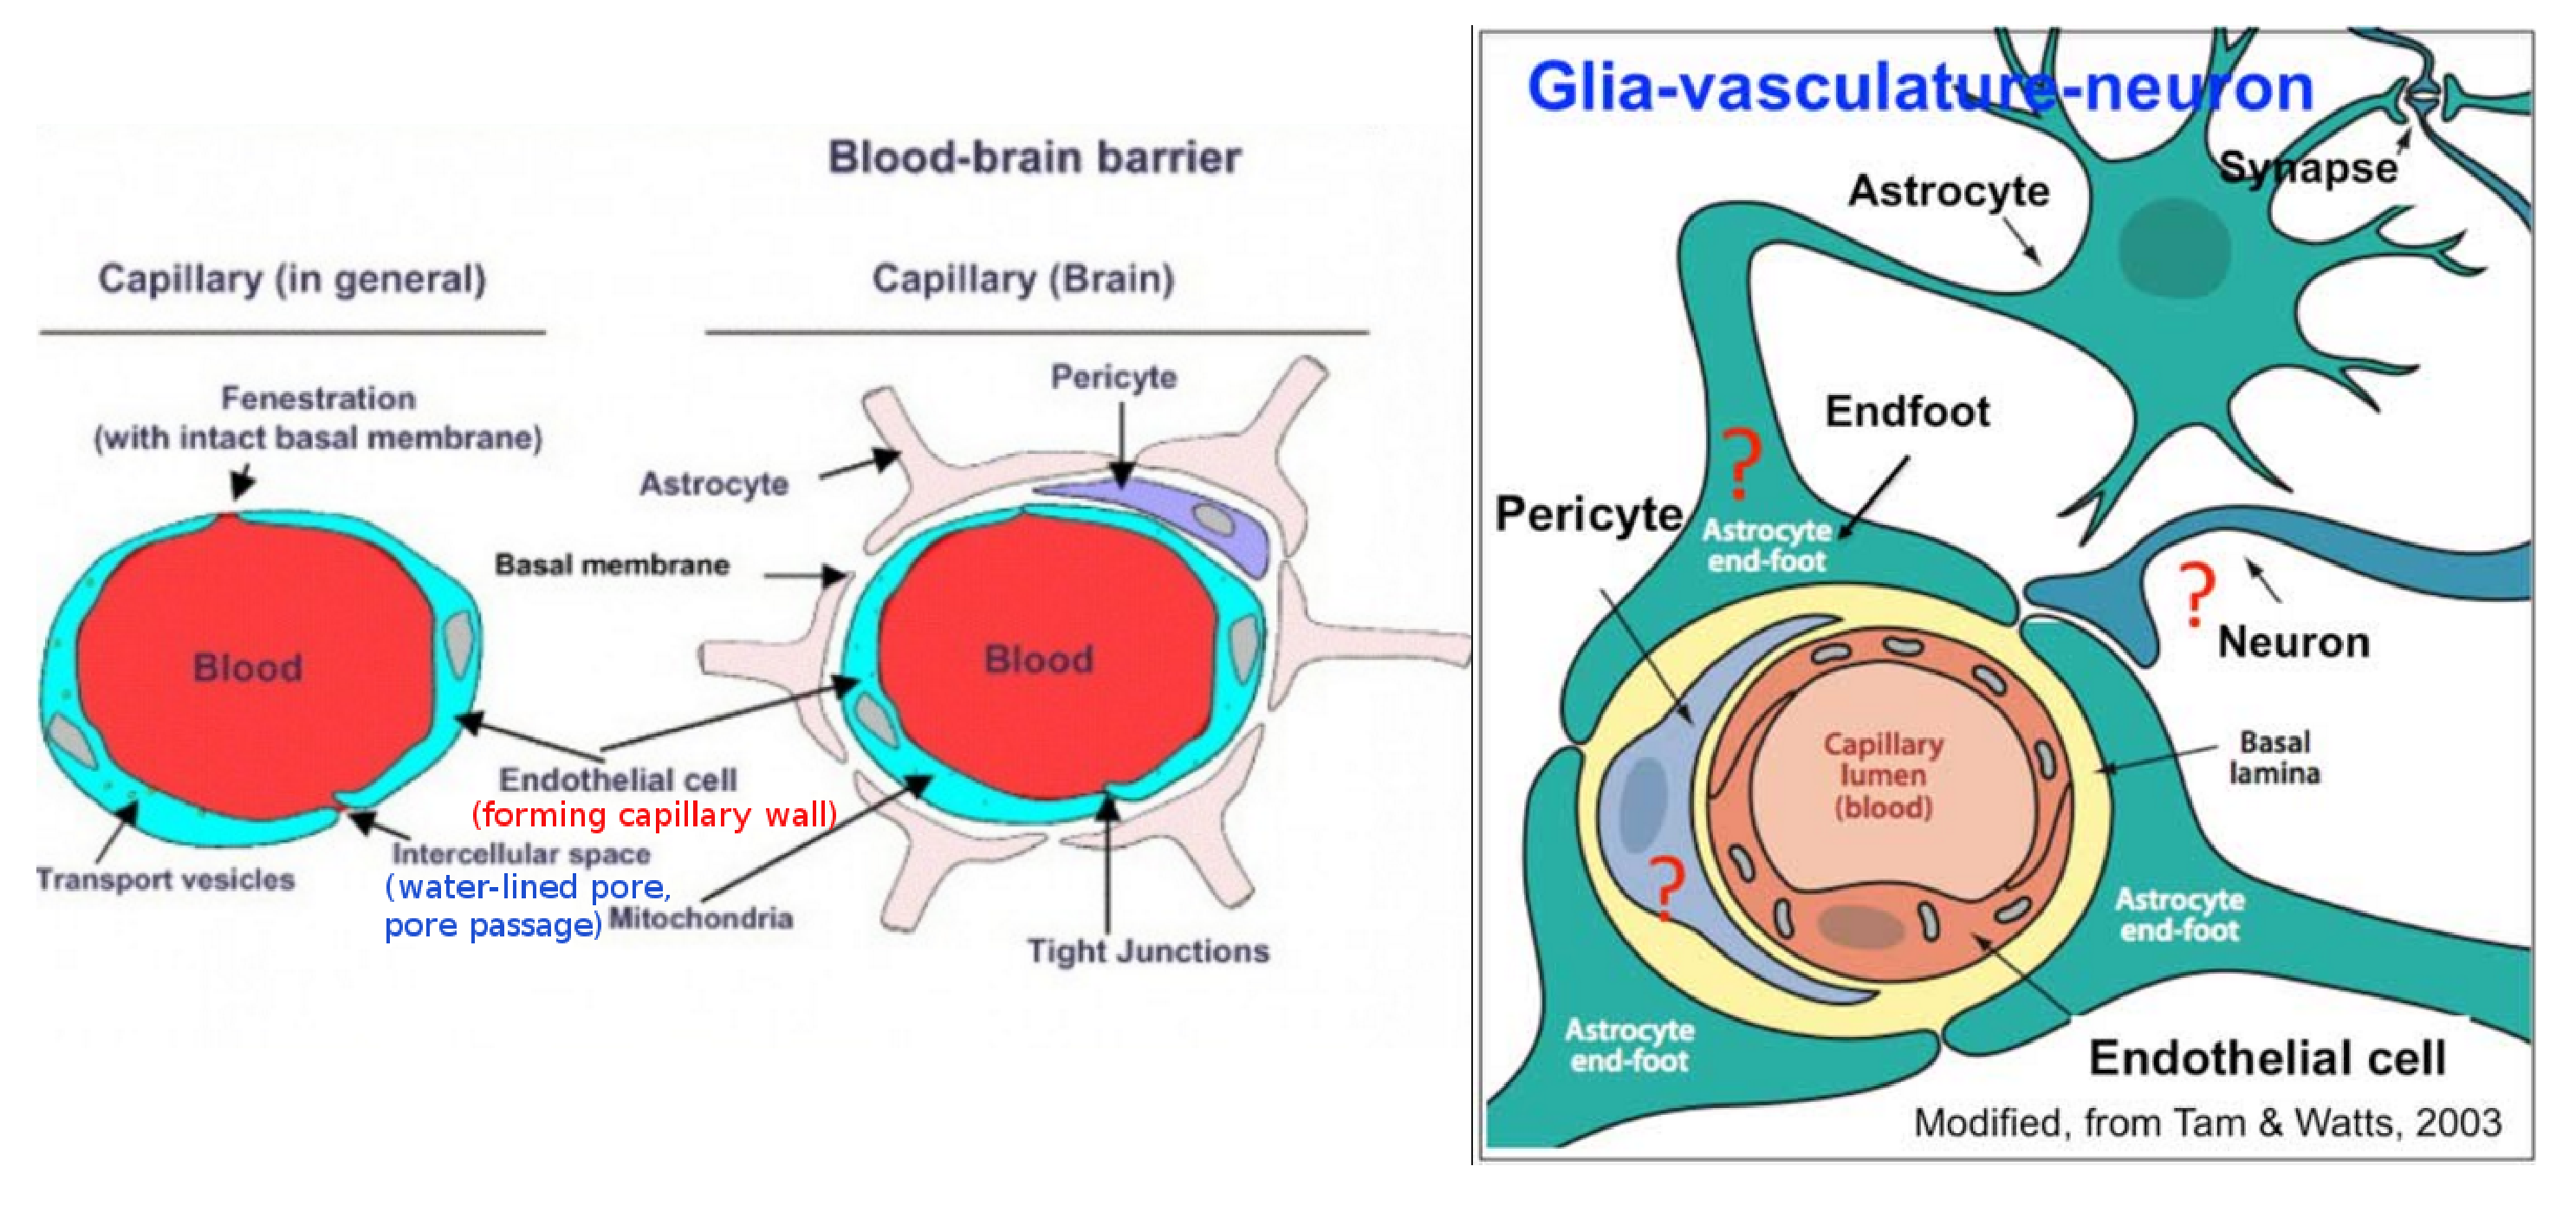
\includegraphics[height=5cm,
    angle=0]{./images/blood-brain-barrier.eps}}
\caption{The endothelial cell layer form tight junctions}
\label{fig:blood-brain-barrier}
\end{figure}


As shown in Fig.\ref{fig:blood-brain-barrier-2}, a portion of the brain
capillary wall, {\bf pericytes} are enclosed within the endothelial basal
lamina, and form the closed association with endothelial cell.
\begin{itemize}
  \item  The endfeet of astrocytic glial cells are apposed to the outer surface of basal
lamina. Sect.\ref{sec:astrocyte-perivascular-endfeet}

  \item In the perivascular space are found microglia, the synaptic terminals and
boutons of nerve fibres, and (in arterioles) smooth muscle cells.

  \item In the larger vessels, cells of the meninges form a perivascular cuff or
  sheath that projects down from the brain surface and demarcates the
  Virchow-Robin space (not show).

\begin{figure}[hbt]
  \centerline{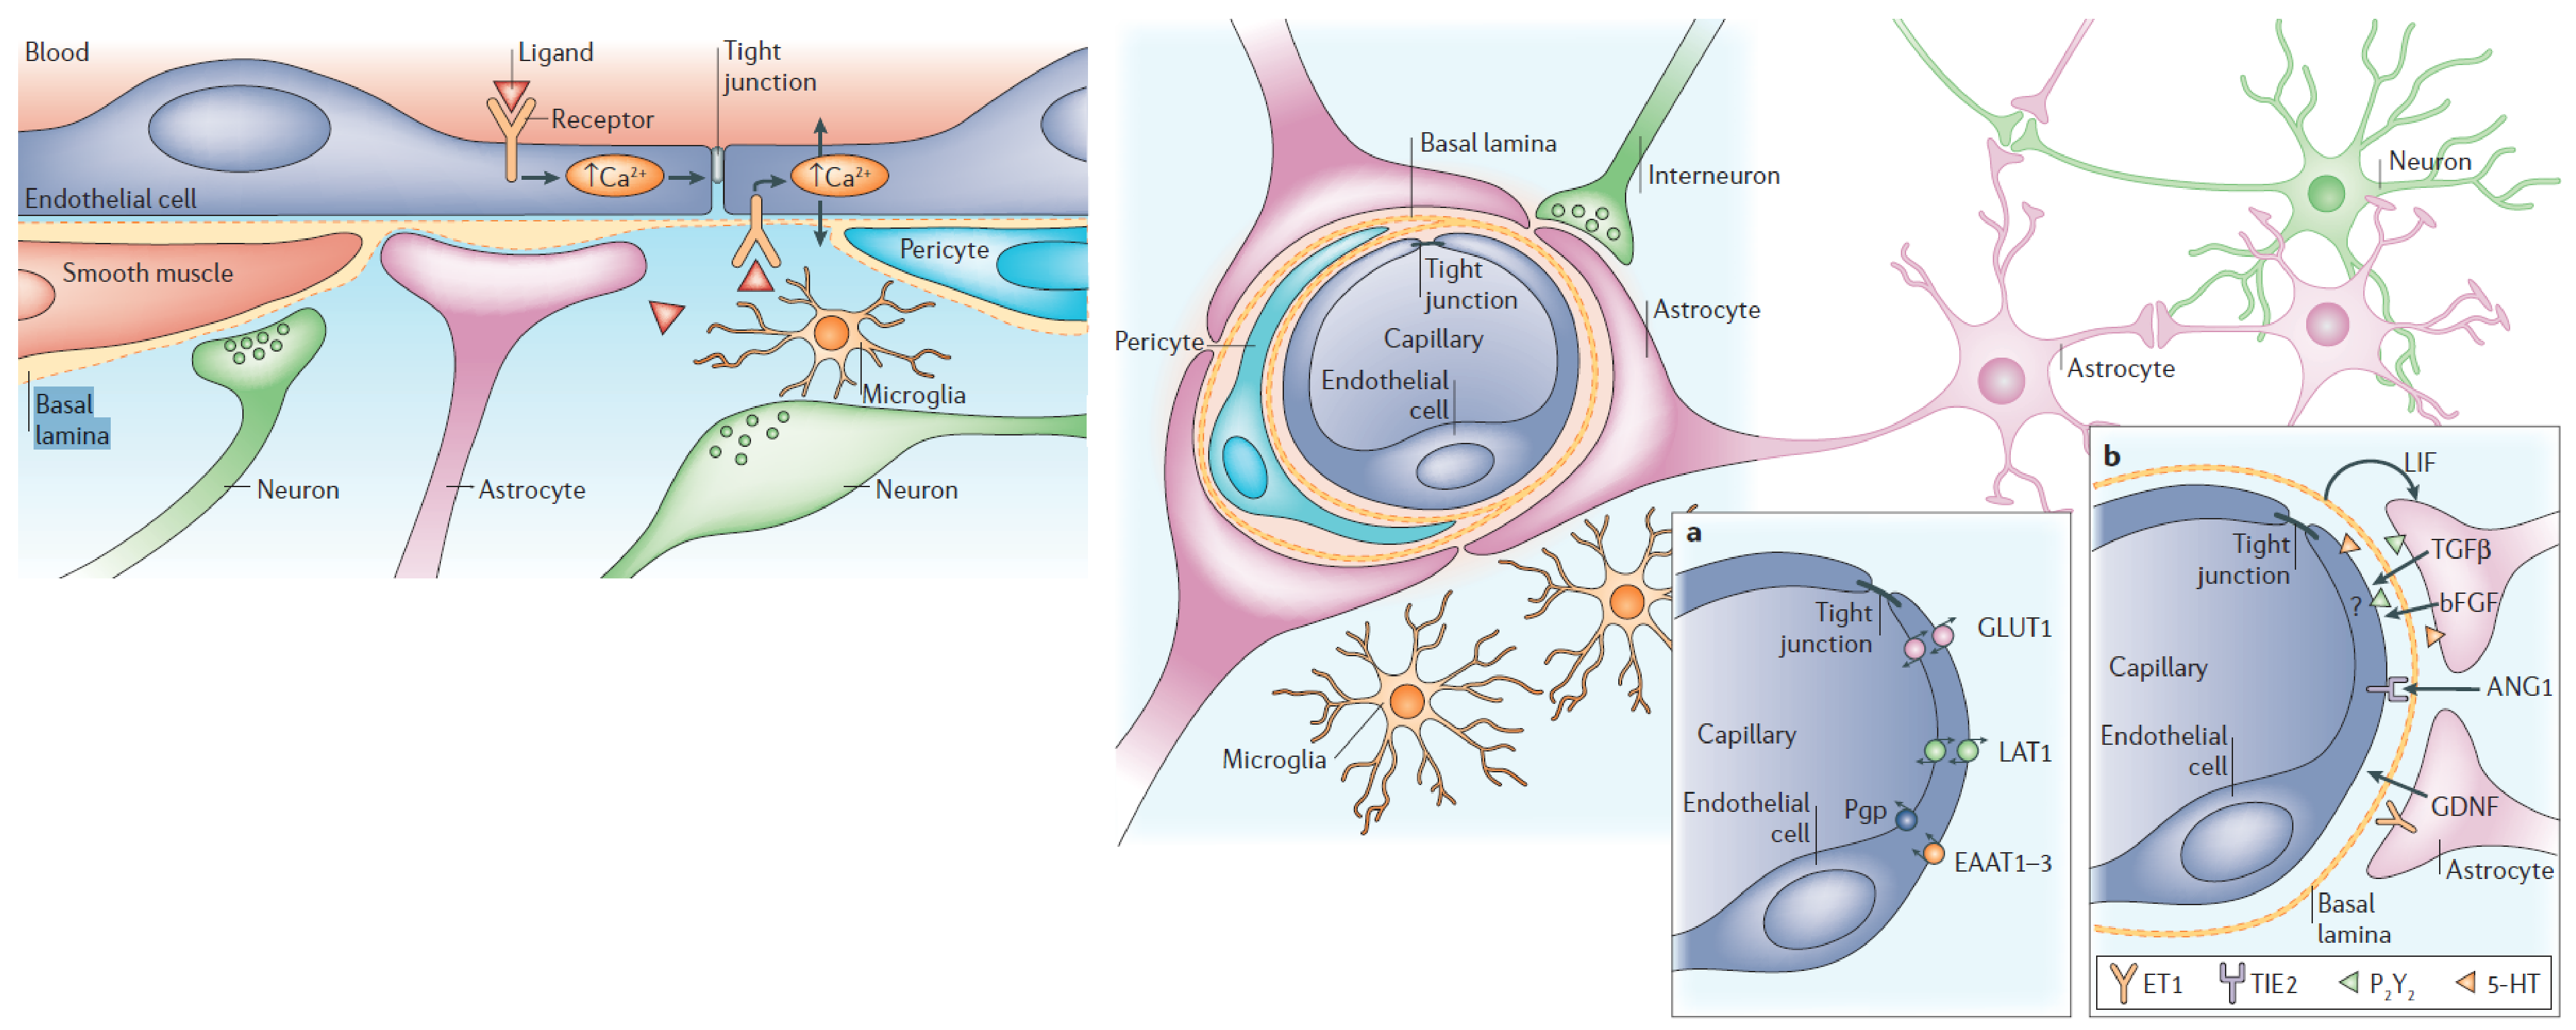
\includegraphics[height=5cm,
    angle=0]{./images/blood-brain-barrier-2.eps}}
\caption{Cellular constituents of blood-brain barrier (Abbott, Hansson, 2006):
GLUT1, LAT1, EAAT1-3, Pgp (P-glycoprotein)}
\label{fig:blood-brain-barrier-2}
\end{figure}

  \item Some receptors are coupled to increases in the concentration of
  intracellular Ca2+

\end{itemize}

Agents such as ATP and histamine can influence endothelial function by
ligand-receptor interaction, from the blood or the brain side.

 \subsection{-- pathogenesis}

P-glycoprotein is a gatekeeper in the blood-brain barrier.

Reduce afficacy of P-glycoprotein in Parkinson's disease:
\begin{itemize}
  \item P-glycoprotein is an ATP-dependent transporter

  \item Elevated uptake of the Pgp substrate (by P-glycoprotein transporter)
  [$^{11}$C]verapamil using PET imaging (Sect.\ref{sec:PET}) in the midbrain
  of patients with Parkinson's disease: this suggest disturbed Pgp function in
  BBB links to Parkinson's disease.
\end{itemize}

The decrease of P-glycoprotein transporter expression level is linked to
accumulation of amyloid-$\beta$ in Alzheimer's disease.

Upregulation of P-glycoprotein expression and other drug efflux transporters in
astrocytes and endothelium in epilepsy: In epilepsy, the normal pattern of brain
ABC transporter expression may change, with upregulation of Pgp on astrocytes
and brain endothelium; this may be an adaptive response to barrier opening (and
hence a less efficient BBB), which is often seen during seizure activity.

\subsection{-- calcium wave in endothelial cell}

Fig.\ref{fig:blood-brain-barrier-2} shows $\Ca$ elevation in one endothelial
cell, and trigger $\Ca$ elevation in the next cell.



\subsection{capillaries}
\label{sec:capillaries}

{\bf capillaries} are the smallest (i.e. around 5-10$\mu$m in diameter) of the
body's blood vessels, with the endothelial linings are only 1 endothelium cell
layer thick (Sect.\ref{sec:endothelial-cell}). They enable  the exchange of
water, oxygen, carbon dioxide, and many other nutrients and waste substances
between the blood and the tissues surround thems.

There is also {\bf pericyte} - a cell of mesodermal origin, and
contractile-phagocytic phenotype, that is associated with the outer surface of
capillaries. It is believed that the interaction between the three cell
types: pericyte, endothelial cells, and astrocytes, are required for proper
cerebral capillary differentiation {\it in vivo}.

\subsection{tight junction between endothelial cell}

Our understanding of the molecular structure of tight junctions derives from
studies of both epithelia and endothelia.
In epithelial cells, tight and adherens junctions are strictly separated from
each other, but in endothelial cells these junctions are intermingled (Review:
Abbott, Hansson, 2006). Cell-cell interaction in the junctional zone is
stabilized by adherens junctions.

\begin{mdframed}

These tight junctions, Fig.\ref{fig:tight-junction-brain-endothelial-cell}
significantly restrict even the movement of small ions ($\Na$, $\Cl$) so that
brain trans-endothelial electrical resistance (TEER) becomes extremely high
($>1,000$ Ohm.cm$^2$); while those in typically endothelial cell is about 2-20
Ohm.cm$^2$ (Review: Abbott, Hasson, 2006).

There is strong evidence that astrocytes (Sect.\ref{sec:astrocytes}) can tighter
tight junctions.
\end{mdframed}



\begin{figure}[hbt]
  \centerline{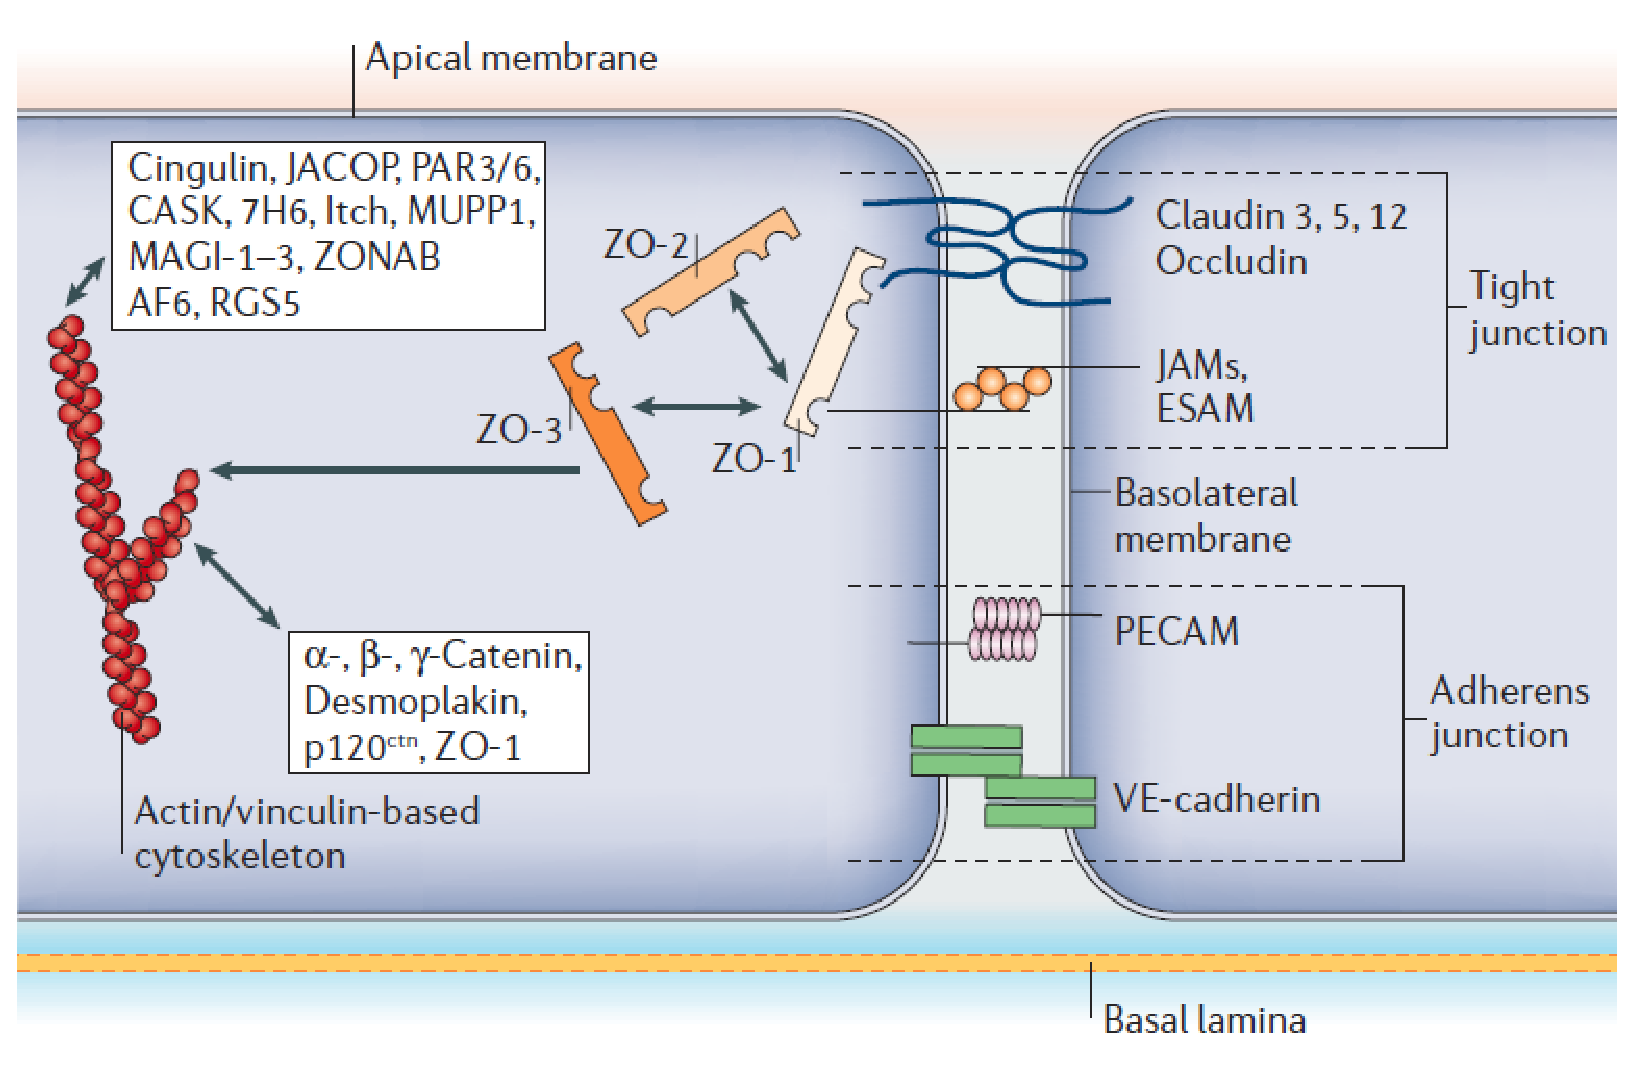
\includegraphics[height=3cm,
    angle=0]{./images/tight-junction-brain-endothelial-cell.eps}}
\caption{The tight junction and adherens junctions between brain endothelial
cells}
\label{fig:tight-junction-brain-endothelial-cell}
\end{figure}


\begin{enumerate}
  \item {\bf occludin}: 60-65 kDa proteins with four transmembrane domains
and two extracellular loops appears for forming tight junctions.

The C-terminal domain of occludin is capable of linking with zonula occulends
protein 1 (ZO-1).

  \item {\bf claudins}: proteins with four transmembrane domains
and two extracellular loops.  {\it claudin 3, claudin 5, } and possibly {\it
claudin 12} appears to contribute to high TEER.


\item junctional adhesion molecules (JAMs) and the endothelial selective adhesion
molecule (ESAM) are members of the immunoglobulin superfamily

JAM-A, JAM-B, and JAM-C are present in brain endothelial cell and are involved
in the formation and maintenance of the tight junctions.

\item Within the cytoplasm are many first-order adaptor proteins, including
zonula occludens 1, 2 and 3 (ZO-1-3) and Ca2+-dependent serine protein kinase
(CASK); MAGI-1, MAGI-2 and MAGI-3 (membrane-associated guanylate kinase with
inverted orientation of protein- protein interaction domains), PAR3, PAR6, and
MUPP1 (multi-PDZ-protein 1):
that bind to the intramembrane proteins (apical membrane with capillaries).

\item The second-order adaptor molecules: among them, cingulin is important, and
junction-associated coiled-coil protein (JACOP) may also be present.

The newly identified protein, junction-associated coiled-coil protein (JACOP),
may anchor the junctional complex to the actin cytoskeleton.
\end{enumerate}

\subsection{endothelial cells}
\label{sec:endothelial-cell}

The endothelial cell, even though a single layer, form complex tight junctionss
between adjacent endothelial cells which force most molecular traffic to take a
trans-cellular route across the BBB (i.e. not able to cross the junction),
rather than moving {\it para-cellularly through the junction}, i.e. from one
endothelial cell to another.



Because of its large surface area ($\approx$ 20 m$^2$ per 1.3 kg brain), and
short diffusion distance between neurons and capillaries, the endothelium has
dominant role in regulating the brain microenvironment.

Small gaseous molecules such as $\ce{O2}$ and $\ce{CO2}$ can diffuse freely
through the lipid membranes, and this is also a route of entry for small
lipophilic agents, including drugs such as barbiturates and ethanol

Endothelial cells can release substances to the blood or brain-side after
receptor activation.

Metabolic barrier formed by a combination of intracellular and extracellular
enzymes:
\begin{enumerate}

  \item {\bf ecto-enzymes}: such as peptidases and nucleotidases are capable of
  metabo lizing peptides and ATP, respectively.

  \item {\bf intracellular enzymes}: monoamine oxidase, cytochrome P450 (1A and
  2B) : inactivate many neuroactive and toxic compounds
\end{enumerate}

\begin{mdframed}

Brain endothelium has a {\it much lower degree} of endocytosis/transcytosis
activity than does peripheral endothelium, which contributes to the transport-barrier
property of the BBB.

\end{mdframed}

Other active/selective transport processes on the luminal
and abluminal membranes (i.e. the endothelial membrane that faces away from the
vessel lumen, and toward the brain)
\begin{enumerate}

  \item {\bf receptor-mediated transcytosis}: transport a specific type of
  large molecules, such as hydrophilic molecules such as peptides and proteins

  \item {\bf adsorptive-mediated transcytosis}: less specific of what it
  transport

  \item GLUT1 - Sect.\ref{sec:GLUT1}: glucose carrier

  \item LAT1 - L-system for large neutral amino acids carrier

  \item transporters for nucleosides, nucleobases, and many other substances

  \item EAAT1-3: excitatory amino acid transporter 1-3 - Sect.\ref{sec:EAAT}
\end{enumerate}


\subsection{basal lamina}
\label{sec:basal-lamina}

{\bf Basal lamina} is the extracellular matrix layer produced by basal cell
membrane, used as an anchoring and signaling site for cell-cell interactions.


\begin{mdframed}
Roche developed the so-called {blood-brain shuttle} which can help to
transport such antibody across the blood vessel into the brain.
The brain shuttle is indeed a special molecule, that can bind to the drug, and
then both will diffuse across the blood vessel.
\url{https://www.youtube.com/watch?v=2JiUPbDtGuQ}

\end{mdframed}

\subsection{brain arterioles and venules}
\label{sec:arterioles}
\label{sec:venules}

Brain arterioles and venules are the larger vessels. There are endothelium of
brain arterioles and venules, although these segments of the microvasculature
may be more leaky and subject to greater modulation that those in brain
capillaries (Sect.\ref{sec:capillaries}).


\subsection{neurovascular units}

{\bf neurovascular units} refers to the organized structure of neurons, glia,
and microvessels, which are involved in the regulation of cerebral blood flow.

Individual neurons are rarely more than 8-20 $\mu$m from the brain capillary;
although they may be milimeters or centimeters from CSF compartment.

\subsection{gliovascular units}

{\bf gliovascular units} refer to the modular structure within a single
neurovascular unit.  In a glialvascular unit, individual astrocytic glia support
the function of particular neuronal populations and territories, and communicate
with associated segments of the microvasculature.




\section{Energy requirement: (post)synaptic potential vs. action potential}

Maintenance and restoration of ion gradients dissipated by signaling processes
such as postsynaptic and action potentials, as well as uptake and recycling of
neurotransmitters, are the main processes contributing to the high brain energy
needs (Attwell and Laughlin, 2001 and Alle et al., 2009).

Among them, synaptic potentials, rather than action potentials, appear to
represent by far the main energetic cost related to maintenance of excitability
(Alle et al., 2009).

white matter, which has a much lower average
metabolic rate than gray matter


In early studies: the fraction of resting energy devoted to signaling, i.e.
neuronal firing of glutamatergic neurons (Sect.\ref{sec:glutamatergic_neurons}),
was quite low.

{\bf In rodents}: since early 2000, many recent experimental studies in rodents
and theoretical modeling have converged on the conclusion that majority of the
resting energy consumption supports glutamatergic signaling and the energy
demand changes linearly with pyramidal neuron firing rates and glutamate
neurotransmitter release and reuptake.

{\bf In (awake) humans}: the fraction of resting
energy usage devoted to glutamatergic signaling is less well
understood.


The energy requirements of the brain are very high, and tight regulatory
mechanisms operate to ensure adequate spatial and temporal delivery of energy
substrates in register with neuronal activity.
Astrocytes-a type of glial cell-have emerged as active players in brain energy
delivery, production, utilization, and storage.

\section{Energy requirements: human vs. rat}

Rodent (13)C magnetic resonance spectroscopy studies show that glutamatergic
signaling requires high oxidative energy in the awake resting state

Many data in rats showed that there is a tight couple between oxidative demand

\section{Traumatic Brain Injury (TBI) or craniocerebral trauma}
\label{sec:TBI}
\label{sec:Traumatic-Brain-Injury}

The term 'traumatic brain injury' (TBI) embodies a heterogeneous array of brain
pathologies affecting an estimated 1.5 million Americans per year and is a major
cause of death (more than 50\% of trauma-related death) and disability in
children and young adults (Ghajar, 2000; Dutton et al., 2010).
% Ghajar J. Traumatic brain injury. Lancet. 2000;356:923-929.
% 2. Dutton RP, Stansbury LG, Leone S, Kramer E, Hess JR, Scalea TM.
% Trauma mortality in mature trauma systems: are we doing better? An
% analysis of trauma mortality patterns, 1997-2008. J Trauma. 2010;69:
% 620-626

According to CDC, there are about 1.5mil people in US suffer from TBI each year.
More than 50,000 people die from TBI each year (Kraus, 1996) and 85,000 people
suffer long term disabilities. 
% Kraus JF, McArthur DL. Epidemiologic aspects of brain injury. Neurol
% Clin. 1996;14:435- 450
In the U.S., more than 5.3 million people live with disabilities caused by TBI.
For US veterans, 20\% of veterans returning from deployment to Iraq and
Afghanistan have TBI. In addition to the prevalence of TBI in military
personnel, there is increasing awareness of TBI in athletic injuries.
Each year, some 300,000 sports-related traumatic injuries, mostly concussions,
occur in the United States.
Concussions represented 8.9\% of all high school athletic injuries and 5.8\% of
all collegiate athletic injuries, the rates being highest in football and
soccer.

\subsection{mTBI: severity}
\label{sec:mTBI}

TBI induces temporary or permanent impairment of cognition, physical function,
and psychosocial behavior. TBI severity ranges widely depending on the nature of
the injury. Among a wide spectrum of TBI sequelae, sensory and cognitive
deficits are some of the most common.
\begin{enumerate}
  \item  auditory dysfunction following injury
includes both peripheral deficits, e.g., increased hearing thresholds,
as well as difficulties with more sophisticated auditory
tasks, such as discriminating sounds in noisy environments or comprehending
speech
  
  \item visual deficits: include blurred vision,
headache, motion sickness, or loss of concentration during visual
task performance
 
 \item sensory deficits: olfaction, which does not involve significant feedback
 with subcortical structures, is also impacted by TBI, and the degree of anosmia
 (i.e. the loss of the sense of smell, either total or partial) is correlated
 with the severity of injury.

\end{enumerate}

The majority of these injuries are classified as mild TBI (mTBI), which are
challenging to diagnose and track because quantitative biomarkers for mTBI are
lacking. mTBI currently cannot be validated through standard methods of clinical
imaging.

\subsection{cause: primary insult}
\label{sec:TBI-primary-insult}

Traumatic brain injury (TBI) refers to brain dysfunction caused by an outside
force, usually a violent blow to the head. Prevention of TBI is the best
approach since there is no cure for now. However, if TBI occurs, then management
of TBI and prevention of secondary insult is the current hope
(Sect.\ref{sec:TBI-detection}).

The causes of TBI are diverse, with 3 top causes: car accident, firearms and
falls.
\begin{enumerate}
  \item  Open head Injury: e.g. bullet wounds, focal damage, penetration of the
  skull

  \item Closed Head Injury, e.g. motor vehicle crashes, slip and fall, focal
  damage and diffuse damage to axons

  \item Deceleration Injuries (Diffuse Axonal Injury):

During the fast movement of the skull through space (acceleration) and the rapid
discontinuation of this action when the skull meets a stationary object
(deceleration) causes the brain to move inside the skull.  The brain moves at a
different rate than the skull because it is soft.

Different parts of the brain move at different speeds because of their relative
lightness or heaviness. The differential movement of the skull and the brain
when the head is struck results in direct brain injury, due to diffuse axonal
shearing, contusion and brain swelling.

{\bf Diffuse axonal shearing}: when the brain is slammed back and forth inside
the skull it is alternately compressed and stretched because of the gelatinous
consistency.  The long, fragile axons of the  neurons (single nerve cells in the
brain and spinal cord) are also compressed and stretched.  If the impact is
strong enough, axons can be stretched until they are torn.  This is called
axonal shearing.  When this happens, the neuron dies.  After a severe brain
injury, there is massive axonal shearing and neuron death.


  \item Chemical/Toxic, i.e. metabolic disorder

It occurs when harmful chemicals damage the neurons. Chemicals and toxins can
include insecticides, solvents, carbon monoxide poisoning, lead poisoning, etc.


  \item Hypoxia (lack of oxygen),


If the blood flow is depleted of oxygen, then irreversible brain injury can
occur from anoxia (no oxygen) or hypoxia (reduced oxygen).
It may take only a few minutes for this to occur.
This condition may be caused by heart attacks, respiratory failure, drops in
blood pressure and a low oxygen environment.


  \item Tumors, e.g. caused by cancer can grow on or over the brain

Tumors can cause brain injury by invading the spaces of the brain and causing
direct damage.


  \item Infections: The brain and surrounding membranes are very prone to
  infections if the special blood-brain protective system is breached

Viruses and bacteria can cause serious and life-threatening diseases of the
brain (encephalitis) and meninges (meningitis)


  \item Stroke: If blood flow is blocked through a cerebral vascular accident
  (stroke), cell death in the area deprived of blood will result


If there is bleeding in or over the brain (hemorrhage or hematoma) because of a
tear in an artery or vein, loss of blood flow and injury to the brain tissue by
the blood will also result in brain damage.


\end{enumerate}


\subsection{current methods of detection}
\label{sec:TBI-detection}

Brain injuries do not heal like other injuries. Recovery is a functional
recovery, based on mechanisms that remain uncertain. No two brain injuries are
alike and the consequence of two similar injuries may be very different.

Symptoms may appear right away or may not be present for days or weeks after the
injury. TBI often results in acute metabolic crisis
(Sect.\ref{sec:metabolic-crisis}). However, the etiology and neuropathology of
TBI is still controversial.

TBI associated with acceleration-deceleration forces
\begin{enumerate}
  \item many cases: result in diffuse axonal injury

  \item some cases: lesions to ventral frontal lobe and ventral anterior medial
  temporal areas
\end{enumerate}

The magnitude of the deficit in cerebral energy metabolism after TBI has been
shown to be the best predictor of outcome.

TBI is generally classified as focal damage consisting of anatomical
lesions in brain tissue in the form of contusions, lacerations,
and hemorrhages, which, in some cases, can be detected
by computerized tomography (CT).


TBI without overt anatomical lesions is only partially diagnosable with tensor
magnetic resonance imaging.
While CT and MRI cannot identify the majority of cases of TBI, recent studies
have found that about 30\% of military personnel with putative TBI resulting
from exposure to blasts from explosive devices showed brain abnormalities when
studied by means of diffusion tensor magnetic resonance imaging, a specialized
application of MRI. Unfortunately, use of such sophisticated techniques is not
practical under most field conditions leaving only a clinical evaluation for the
diagnosis of concussion.

TBI resulting from explosive blasts, auto accidents, or athletic injuries
creates diffuse neuronal damage with or without loss of consciousness or
impairment of cognitive function. TBI involves impairment of both cerebral blood
flow and metabolism, with decreased cerebral O2 uptake, increased lactate
production (i.e. increase La/Py ratio), and depletion of brain high-energy
phosphate stores.

The drop in cellular energy leads, in turn, to an increase in intracellular Na+
and Ca2+, excessive release of neurotransmitters, and the initiation of
apoptosis

\subsection{current drugs: Cyclosporine A (CsA)}
\label{sec:cyclosporine-A}

Cyclosporine A, one of the earliest immunosuppressant drugs, acts to mitigate
TBI's adverse effects in man and in laboratory animal models of TBI.

Cyclosporine A is thought to decrease mitochondrial damage by blocking opening
of the mitochondrial permeability transition pore (Sect.\ref{sec:mPTP}).
Cyclosporine has been found to bind specifically to mitochondrial cyclophilin-D.


REID (Wellstat): The beneficial effects of cyclosporine are mediated by its
ability to shut the mito permeability transition pore (preventing cell death,
but not necessarily making neurons undergoing a power brown-out work better);
uridine acts upstream of the MPTP per se to improve bioenergetics and also,
indirectly, to prevent collapse of the mito membrane potential and consequent
apoptotic cell death (without the safety concerns of giving an immunosuppressant
to a trauma patient).





\subsection{chronic traumatic encephalopathy (CTE)}
\label{sec:CTE-chronic-traumatic-encephalopathy}

CTE is a chronic brain syndrome that can give rise to symptoms and signs of
early-onset dementia, including impaired memory, confusion, depression, and
suicide

At present, no treatment aimed at preventing chronic traumatic encephalopathy
(CTE), a possible long-term consequence of TBI, is being implemented.

Evidence continues to mount that individuals who have experienced repeated
concussive and subconcussive head injuries (such as professional boxers and
football players) are also at enhanced risk of developing CTE




\section{Metabolic acidosis}
\label{sec:metabolic-acidosis}

Metabolic acidosis happens when the chemical balance of acids and bases in your
blood gets thrown off.
\begin{itemize}
  \item the body is making too much acid
  \item the body is not getting rid of acid fast enough
  \item the body doesn't have enough base to balance the amount of acid
\end{itemize}
When any of these happen, chemical reactions and processes in your body don't
work right.

Examples:
\begin{enumerate}
  \item lactate acidosis - Sect.\ref{sec:lactate-acidosis}
\end{enumerate}

\section{Metabolic crisis}
\label{sec:metabolic-crisis}

\begin{enumerate}
  \item acute metabolic crisis
  \item chronic metabolic crisis

  \item early metabolic crisis:
\end{enumerate}

\chapter{Models of mitochondria}
\label{chap:mitochondria-cardiac-models}

Sect.\ref{sec:mito_intro}


\section{Ischemia}
\label{sec:heartdisease_ischemia}

To help understand the cell reponse to metabolism under ischemia,
Jafri-Kumar (Sect.\citep{jafri2014}) have built a computational model for the
mitochondria based on the previous model of \citep{abc} to investigate
\begin{enumerate}
  \item Mechanism of mitochondrial acidification in response to cytosolic pH
  changes, and the consequences of this change to mitochondrial membrane
  potential change and calcium uptake rate. CONCLUSION: acidification reduce
  mitochondrial $[\Ca]_m$ overload.
  \item As mainting a proper matrix volume is critical to optimum energy
  production, the model study which parameters control the most to this volume

  \item Provide formula for ROS production in the matrix. ROS is an ischemic
  preconditioning (IPC) mediator providing protection from ischemic-repurfusion
  damage.
\end{enumerate}

The explanation for the increase in $[\Ca]_m$ is as follows: cytosolic
acidification activates sarcolemma $\Na/\H$ exchanger (NHE$_m$), causing
cytosolic $[\Na]_i$ to increase, which in turns activate NCX to pump $\Na$
out and take $\Ca$ in, i.e. increasing $[\Ca]_i$ \citep{orourke2005}.

The rise in $[\Ca]_i$ always parallel with the increase in $[\Ca]_m$
\citep{gurshani2004} which may activate mitochondrial dehydrogenases
(Sect.\ref{sec:dehydrogenase}) which is in turn accompanied by a rise of
reducing NADH, FADH$_2$, increase electron transport to produce more
ATP\citep{mccormack1990}. ATP can also be generated by direct activation of
$[\Ca]_m$ via ATP synthase \citep{territo2000}.

Regardless of its vital role of $[\Ca]_m$, the overload of calcium can be fatal,
e.g. inhibition of oxidative phosphorylation and degrade ATP production
\citep{kovacs2005}. When accompanied by elevated phosphate level, it can cause the
opening of mitochondrial permeability transition pore (MPTP), a nonspecific pore that
open inner membrane of mitochondria, leading to mitochondria swelling.

In addition to $\Ca$, mitochondrial pH level is maintained a proper level with
that in cytosol \citep{baysal1991} (due to proton extrusion by electron
transport chain).
In some situation, e.g. metabolic inhibition when proton transport is greatly
reduced, mitochondrial pH can decrease. This can also affect the regulation of
$[\Ca]_m$ through the orchestring of $\NaH$ exchange and $\NCX$
\citep{baysal1991,nguyen2007}.

Under pathological condition, mitochondrial ATP-sensitive $\K$ channel
($I_\KATP$ or $\mitoATP$) also activate. The opening of this channels protects
the heart against ischemic-reperfusion (IR) injury \citep{kowaltowski2001,
garlid2003}. The transport of $\K$ across mitochondria is crucial for
maintaining volume homeostasis (mediated by $\KH$ antiporter or KHE$_m$), and to
prevent excess matrix contraction. Contraction is energetically unfavorable as it
reduce electron transport chain. The main pathway for $\K$ regulation is $\KHEm$
and the secondary pathway is $\NHEm$.

\section{Numerical methods}


\section{Lund concept}
\label{sec:Lund-concept}


The Lund concept (LC), introduced in 1912, was the first complete guideline for
treatment of severe traumatic brain injury (s-TBI) - those with Glascow Coma
Score 3-8.

LC strives for treatment of the pathophysiological mechanisms behind symptoms
rather than just treating the symptoms.
It is reasonable to assume that making the hypoxic penumbra zone of the injured
brain to survive by optimizing brain perfusion and oxygenation is crucial when
discussing outcome of the brain.  

 
It was a theoretical approach, based mainly on general physiological
principles - i.e., of brain volume control and optimization of brain perfusion and
oxygenation of the penumbra zone.

The concept gave relatively strict outlines for cerebral perfusion pressure,
fluid therapy, ventilation, sedation, nutrition, the use of vasopressors, and
osmotherapy.

The treatment is standardized, with less need for individualization.
Meta-analytic approaches from clinical outcome studies and to some extent from
systematic reviews



%%% Local Variables:
%%% mode: latex
%%% TeX-master: "cardiology"
%%% End:
